\documentclass[12pt,a4paper]{article}
%
%	STARWARE - Stile base per la scrittura di documenti interni in LaTex
%

%
%	Pacchetti globali
%	Fare qui eventuali aggiunte!
%
\usepackage[utf8]{inputenc}
\usepackage[italian]{babel}
\usepackage[babel]{csquotes}
\usepackage{url}
\usepackage{graphicx}
\usepackage[colorlinks]{hyperref}
\usepackage{lastpage}
\usepackage{fancyhdr}
\usepackage[top=1cm,bottom=4cm,left=80pt,right=80pt]{geometry} %disegna la linea
\usepackage{listings} %per grandi porzioni di codice
\usepackage{color}
\usepackage[table]{xcolor}
\usepackage{booktabs,tabularx}
\usepackage{makeidx}
\usepackage{fixltx2e}
\usepackage{hyperref}
\usepackage{enumitem}
\usepackage{color}
\usepackage[T1]{fontenc}
\usepackage{float}
\usepackage{svg}
\usepackage{amsmath}
\usepackage[toc]{glossaries}
\usepackage{dirtree}
\usepackage{listings}

\makeglossaries

\bibliographystyle{alpha}

%
%	VARIABILI GLOBALI
%
\newcommand{\nomeGruppo}{StarWare}
\newcommand{\mailGruppo}{starware.swe@gmail.com}
\newcommand{\uni}{Universit\`{a} degli Studi di Padova}
\newcommand{\uniAA}{2015/2016}
\newcommand{\Cardin}{Prof. Riccardo Cardin}
\newcommand{\Vardanega}{Prof. Tullio Vardanega}
\newcommand{\Zucchetti}{Zucchetti S.p.a.}
\newcommand{\prj}{Quizzipedia}
\newcommand{\prjL}{Quizzipedia: software per la gestione di questionari}

\newcommand{\AVI}{Alessio Vitella}
\newcommand{\AVE}{Andrea Venier}
\newcommand{\NDC}{Nicola De Cao}
\newcommand{\IB}{Igor Baylyak}
\newcommand{\WS}{Walter Sandon}
\newcommand{\TP}{Thomas Pigarelli}
\newcommand{\AB}{Anna Bonaldo}

\newcommand{\mgls}[1]{\gls{#1}\textsubscript{G}}
\newcommand{\mglspl}[1]{\glspl{#1}\textsubscript{G}}
\newcommand{\mGls}[1]{\Gls{#1}\textsubscript{G}}
\newcommand{\mGlspl}[1]{\Glspl{#1}\textsubscript{G}}

\newcommand{\AM}{\emph{\mGls{amministratore}}}
\newcommand{\AN}{\emph{\mGls{analista}}}
\newcommand{\PG}{\emph{\mGls{progettista}}}
\newcommand{\PR}{\emph{\mGls{programmatore}}}
\newcommand{\VR}{\emph{\mGls{verificatore}}}
\newcommand{\PM}{\emph{\mGls{project manager}}}

\newcommand{\AMpl}{\emph{\mGlspl{amministratore}}}
\newcommand{\ANpl}{\emph{\mGlspl{analista}}}
\newcommand{\PGpl}{\emph{\mGlspl{progettista}}}
\newcommand{\PRpl}{\emph{\mGlspl{programmatore}}}
\newcommand{\VRpl}{\emph{\mGlspl{verificatore}}}
\newcommand{\PMpl}{\emph{\mGlspl{project manager}}}

\newcommand{\RR}{\emph{\mGls{revisione dei requisiti}}}
\newcommand{\RA}{\emph{\mGls{revisione di accettazione}}}
\newcommand{\RP}{\emph{\mGls{revisione di progettazione}}}
\newcommand{\RQ}{\emph{\mGls{revisione di qualifica}}}

\newcommand{\NdP}{\emph{\mGls{norme di progetto}}}
\newcommand{\SdF}{\emph{\mGls{stidio di fattibilita}}}
\newcommand{\AdR}{\emph{\mGls{analisi dei requisiti}}}
\newcommand{\PdP}{\emph{\mGls{piano di progetto}}}
\newcommand{\PdQ}{\emph{\mGls{piano di qualifica}}}

\newcommand{\latex}[1]{\texttt{#1}}
\newcommand{\fileName}[1]{\texttt{#1}}
\newcommand{\filePath}[1]{\texttt{#1}}
\newcommand{\TODO}[1]{\texttt{\large \color{red} \underline{TODO: #1}}}

\newcommand{\licenza}{GNU GENERAL PUBLIC LICENSE V2}

%per compilare il template usare questi sotto e commentare glia altri:
%\newcommand{\logoLungo}{../imgs/logoLungo.png}
%\newcommand{\logoGrande}{../imgs/logoGrande.png}
\newcommand{\logoLungo}{../../../template/imgs/logoLungo.png}
\newcommand{\logoGrande}{../../../template/imgs/logoGrande.png}

%
%	Setup stili
%

\newcommand{\HRule}{\rule{\linewidth}{0.5mm}}

\definecolor{dkgreen}{rgb}{0,0.6,0}
\definecolor{gray}{rgb}{0.5,0.5,0.5}
\definecolor{mauve}{rgb}{0.58,0,0.82}
\definecolor{light}{RGB}{255,255,190}

%
%	Setup di pagina
%

%colorazione link
\hypersetup
{
	colorlinks=true,
	linkcolor=black,
	urlcolor=blue,
	citecolor=blue
}

%	Setup Header + Footer

\pagestyle{fancy}
\setlength{\headheight}{2cm} %settato grandezza header

\renewcommand{\footrulewidth}{0.5pt} %ridefinisco il valore della riga di intestazione
\renewcommand{\headrulewidth}{0.5pt} %ridefinisco il valore della riga di pie' di pagina
\addtolength{\headwidth}{\marginparsep}
\addtolength{\headwidth}{\marginparwidth}

\fancyhead{} %annulla head di default
\fancyfoot{} %annulla foot di default

%	Logo intestazione
\lhead{
\includegraphics[scale=0.12]{\logoLungo}}


%	footer
\cfoot{
	\uni \ - \uniAA \\
	\href{mailto:\mailGruppo}{\mailGruppo}\\
	{\tiny Questo documento è distribuito sotto licenza {\licenza}}
}
\rfoot{
	\thepage\ di \pageref{LastPage}
}


% test subsubsubsection

\usepackage{titlesec}
\usepackage{hyperref}

\titleclass{\subsubsubsection}{straight}[\subsection]

\newcounter{subsubsubsection}[subsubsection]
\renewcommand\thesubsubsubsection{\thesubsubsection.\arabic{subsubsubsection}}
\renewcommand\theparagraph{\thesubsubsubsection.\arabic{paragraph}} % optional; useful if paragraphs are to be numbered

\titleformat{\subsubsubsection}
  {\normalfont\normalsize\bfseries}{\thesubsubsubsection}{1em}{}
\titlespacing*{\subsubsubsection}
{0pt}{3.25ex plus 1ex minus .2ex}{1.5ex plus .2ex}

\makeatletter
\renewcommand\paragraph{\@startsection{paragraph}{5}{\z@}%
  {3.25ex \@plus1ex \@minus.2ex}%
  {-1em}%
  {\normalfont\normalsize\bfseries}}
\renewcommand\subparagraph{\@startsection{subparagraph}{6}{\parindent}%
  {3.25ex \@plus1ex \@minus .2ex}%
  {-1em}%
  {\normalfont\normalsize\bfseries}}
\def\toclevel@subsubsubsection{4}
\def\toclevel@paragraph{5}
\def\toclevel@paragraph{6}
\def\l@subsubsubsection{\@dottedtocline{4}{7em}{4em}}
\def\l@paragraph{\@dottedtocline{5}{10em}{5em}}
\def\l@subparagraph{\@dottedtocline{6}{14em}{6em}}
\makeatother

\setcounter{secnumdepth}{4}
\setcounter{tocdepth}{4}


%pdflatex -synctex=1 -interaction=nonstopmode %.tex|makeglossaries %|pdflatex -synctex=1 -interaction=nonstopmode %.tex|pdflatex -synctex=1 -interaction=nonstopmode %.tex
\makeglossary

\newglossaryentry{responsabile} {
	name=responsabile,
	description={è il responsabile della gestione, pianificazione e realizzazione del progetto},
	plural=Responsabili
}

\newglossaryentry{verificatore} {
	name=verificatore,
	description={è il responsabile dell'attività di verifica},
	plural=Verificatori
}

\newglossaryentry{programmatore} {
	name=programmatore,
	description={è responsabile delle attività di codifica miranti alla realizzazione del prodotto e delle componenti di ausilio necessarie per l'esecuzione delle prove di verifica e validazione},
	plural=programmatori
}

\newglossaryentry{progettista} {
	name=progettista,
	description={è responsabile delle attività di progettazione},
	plural=Progettisti
}

\newglossaryentry{analista} {
	name=analista,
	description={è responsabile delle attività di analisi. },
	plural=Analisti
}

\newglossaryentry{amministratore} {
	name=amministratore,
	description={è responsabile dell'efficienza e dell'operatività dell'ambiente di sviluppo; si occupa della redazione e attuazione di piani e procedure di gestione della qualità; inoltre gestisce l'archivio della documentazione del progetto},
	plural=Amministratori
}

\newglossaryentry{revisione dei requisiti} {
	name=revisione dei requisiti,
	description={è una revisione formale che determina l'accesso del gruppo al progetto didattico e la concordanza con il cliente di una visione condivisa del prodotto atteso}
}

\newglossaryentry{revisione di accettazione} {
	name=revisione di accettazione,
	description={è una revisione formale per l'accertamento del soddisfacimento di tutti i requisiti e il completamento del progetto}
}

\newglossaryentry{revisione di progettazione} {
	name=revisione di progettazione,
	description={è una revisione di progresso che accerta la realizzabilità del prodotto e informa il cliente sulle caratteristiche del prodotto}
}

\newglossaryentry{revisione di qualifica} {
	name=revisione di qualifica,
	description={è una revisione di progresso che approva l'esito finale delle verifiche e attiva la fase di validazione}
}

\newglossaryentry{analisi} {
	name=analisi,
	description={è il periodo di preparazione e produzioni di documenti che precede la Revisione dei requisiti}
}

\newglossaryentry{progettazione} {
	name=progettazione,
	description={è il periodo che intercorre tra la Revisione dei requisiti e la Revisione di progettazione}
}

\newglossaryentry{codifica} {
	name=codifica,
	description={è il periodo che intercorre tra la Revisione di progettazione e la Revisione di qualifica}
}

\newglossaryentry{validazione} {
	name=validazione,
	description={è il periodo che intercorre tra la Revisione di qualifica e la Revisione di accettazione}
}

\newglossaryentry{repository} {
	name=repository,
	description={è dove i file sono memorizzati, spesso su un server}
}

\newglossaryentry{ruolo} {
	name=ruolo,
	description={una delle figure professionali che una persona fisica interpreta nel corso del progetto. I ruoli sono: responsabile, amministratore, analista, progettista, programmatore e verificatore},
    plural=ruoli
}

\newglossaryentry{svg} {
	name=SVG,
	description={è un formato per la visualizzazione di oggetti in grafica vettoriale. Per maggiori informazioni si veda \href{https://it.wikipedia.org/wiki/Scalable_Vector_Graphics}{qui}}
}

\newglossaryentry{png} {
	name=PNG,
	description={abbreviazione di Portable Network Graphics, è un formato di file per memorizzare immagini. Per ulteriori informazioni si veda \href{http://it.wikipedia.org/wiki/Portable_Network_Graphics}{qui}}
}

\newglossaryentry{pdf} {
	name=PDF,
	description={è un formato di file basato su un linguaggio di descrizione di pagina sviluppato da Adobe Systems nel 1993 per rappresentare documenti in modo indipendente dall’hardware e dal software utilizzati per generarli o per visualizzarli. Per ulteriori informazioni si veda \href{http://it.wikipedia.org/wiki/Portable_Document_Format}{qui}}
}

\newglossaryentry{uml} {
	name=UML,
	description={è un linguaggio di modellazione e specifica basato sul paradigma object-oriented. Per ulteriori informazioni si veda \href{http://it.wikipedia.org/wiki/Unified_Modeling_Language}{qui}}
}

\newglossaryentry{walkthrough} {
	name=walkthrough,
    description={consiste nella lettura di un documento o codice cercando errori ed anomalie senza un'idea precisa di quali tipi di errori sarà possibile trovare}
}

\newglossaryentry{lista di controllo} {
	name=lista di controllo,
	description={è un elenco di cose da fare per eseguire una determinata attività}
}

\newglossaryentry{inspection} {
	name=inspection,
	description={è la lettura mirata di un documento o codice cercando errori specifici}
}

\newglossaryentry{milestone} {
	name=milestone,
	description={momento saliente nello sviluppo di un prodotto software per la quale devono essere pronti documenti e/o funzionalità}
}

\newglossaryentry{ticket} {
	name=ticket,
	description={rappresenta un compito nell'organizzazione e distribuzione del lavoro all'interno del progetto},
	plural=tickets
}

\newglossaryentry{commit} {
	name=commit,
	description={è la copia di modifiche fatte su file locali verso la repository remota. Esso rappresenta anche un particolare stato della repository nel tempo}
}

\newglossaryentry{versionamento} {
	name=versionamento,
	description={è la gestione di un versioni multiple di un insieme di informazioni. Per maggiori informazioni si veda \href{http://it. wikipedia.org/wiki/Controllo_versione}{qui}}
}

\newglossaryentry{task} {
	name=task,
	description={è un compito secondo la definizione dello standard IEEE 12207},
	plural=tasks
}

\newglossaryentry{attivita} {
	name=attivita,
	description={è un insieme di task}
}

\newglossaryentry{redattore} {
	name=redattore,
	description={colui che redige un documento},
	plural=redattori
}

\newglossaryentry{proponente} {
	name=proponente,
	description={colui che ha proposto al committente un capitolato d'appalto}
}

\newglossaryentry{committente} {
	name=committente,
	description={colui che assegna un compito. In questo caso è il Professor Tullio Vardanega}
}

\newglossaryentry{quality assurance} {
	name=quality assurance,
	description={è l'insieme delle attività volte a garantire il soddisfacimento degli obiettivi della qualità}
}

\newglossaryentry{telegram} {
	name=telegram,
	description={è un servizio di messaggistica istantanea utilizzato dal gruppo per comunicazioni interne. Per maggiori informazioni si veda \href{https://it.wikipedia.org/wiki/Telegram_(software)}{qui}}
}

\newglossaryentry{browser} {
	name=browser,
	description={è un'applicazione per il recupero, la presentazione e la navigazione di risorse web}
}

\newglossaryentry{google drive} {
	name=Google Drive,
	description={è un servizio di memorizzazione e sincronizzazione online introdotto da Google il 24 aprile 2012. Per maggiori informazioni si veda \href{https://it.wikipedia.org/wiki/Google_Drive}{qui}}
}

\newglossaryentry{skype} {
	name=Skype,
	description={è un software proprietario freeware di messaggistica istantanea e VoIP. Per maggiori informazioni si veda \href{https://it.wikipedia.org/wiki/Skype}{qui}}
}

\newglossaryentry{gantt} {
	name=Gantt,
	description={è un diagramma di supporto alla gestione dei progetti}
}

\newglossaryentry{projectlibre} {
	name=ProjectLibre,
	description={è un software di gestione progettuale}
}

\newglossaryentry{pert} {
	name=PERT,
	description={è uno strumento volto alla programmazione delle attività che compongono il progetto e, più in generale, alla gestione degli aspetti temporali di quest'ultimo}
}

\newglossaryentry{subtask} {
	name=subtask,
	description={è un task compreso all'interno di un altro task. La totalità di tutti i subtasks costituisce un intero task}
	plural=subtasks
}

\newglossaryentry{ticketing} {
	name=ticketing,
	description={procedura con la quale il Responsabile assegna un task}
}

\newglossaryentry{git} {
	name=git,
	description={è un sistema software di controllo di versione distribuito}
}

\newglossaryentry{quizzpedia} {
	name=Quizzpedia,
	description={è il nome del prodotto software richiesto dal capitolato d'appalto scelto}
}

\newglossaryentry{schierabile} {
	name=schierabile,
	description={è la capacità di rilasciare al cliente, con relativa installazione e messa in funzione o esercizio, di una applicazione o di un sistema software tipicamente all'interno di un sistema informatico aziendale}
}

\newglossaryentry{cross-platform} {
	name=cross-platform,
	description={può essere riferito ad un linguaggio di programmazione, ad un'applicazione software o ad un dispositivo hardware che funziona su più di un sistema}
}

\newglossaryentry{qml} {
	name=QML,
	description={è un "Domain Specific Language" richiesto dal capitolato d'appalto per la definizione delle domande all'interno del sistema}
}

\newglossaryentry{tomcat} {
	name=Tomcat,
	description={è un application server nella forma di contenitore servlet open source sviluppato dalla Apache Software Foundation. Per maggiori informazioni si veda \href{https://it.wikipedia.org/wiki/Apache_Tomcat}{qui}}
}

\newglossaryentry{java} {
	name=Java,
	description={è un linguaggio di programmazione orientato agli oggetti, specificatamente progettato per essere il più possibile indipendente dalla piattaforma di esecuzione. Per maggiori informazioni si veda \href{https://it.wikipedia.org/wiki/Java_(linguaggio_di_programmazione)}{qui}}
}

\newglossaryentry{node.js} {
	name=Node.js,
	description={è un framework che permette di realizzare web application usando un linguaggio di programmazione che utilizza la stessa sintassi di JavaScrip. Utilizza un modello event-driven, anzichè il classico modello a processi o thread concorrenti, e ciò significa che si eseguono azioni solo al verificarsi di un evento. Questo modello asincrono rende leggero ed efficiente, ideale per applicazioni real-time in per dispositivi distribuiti}
}

\newglossaryentry{javascript} {
	name=JavaScript,
	description={linguaggio di scripting orientato agli oggetti comunemente usato nella programmazione
Web}
}

\newglossaryentry{postgresql} {
	name=PostgreSQL,
	description={e un sistema di gestione di basi di dati open source usato per applicazioni che richiedono caratteristiche molto complesse complesse}
}

\newglossaryentry{mongodb} {
	name=MongoDB,
	description={è un sistema gestionale di basi di dati NoSQL orientato ai documenti, adatto per ambienti che hanno la necessità d'immagazzinare grosse quantità di dati, e dove il linguaggio utilizzato per la gestione dei dati è \mgls{javascript}}
}

\newglossaryentry{html5} {
	name=HTML5,
	description={linguaggio di markup per la strutturazione delle pagine web}
}

\newglossaryentry{css3} {
	name=CSS3,
	description={è un linguaggio di programmazione web utilizzato per descrivere l'aspetto e la formattazione di un sito web al browser lato client. }
}

\newglossaryentry{xml} {
	name=XML,
	description={è un meta-linguaggio che fornisce un insieme standard di regole sintattiche per modellare la struttura di documenti e dati. Questo insieme di regole, definiscono le modalità secondo cui è possibile crearsi un proprio linguaggio di markup}
}

\newglossaryentry{nosql} {
	name=NoSQL,
	description={come dice anche il termine questi database non sono basati su SQL, non sono basati su uno schema relazionale. I database relazionali sono infatti ottimi quando esistono delle relazioni tra i dati che salviamo, ma sono poco performanti nel caso sia necessario salvare una grande quantità di dati, magari usando la scalabilità orizzontale, quando cioè si utilizzano più server dove salvare questi dati e non solamente incrementando la potenza di un singolo server.
}
}

\newglossaryentry{scala} {
	name=Scala,
	description={è un linguaggio di programmazione di tipo general-purpose multi-paradigma studiato per integrare le caratteristiche e funzionalità dei linguaggi orientati agli oggetti e dei linguaggi funzionali. Per maggiori informazioni si veda \href{https://it.wikipedia.org/wiki/Scala_(linguaggio_di_programmazione)}{qui}}
}

\newglossaryentry{akka} {
	name=Akka,
	description={è un toolkit di strumenti per la costruzione di applicazioni con elevata concorrenza di dati che necessitano di un sistema resilente per l'invio e la ricezione di messaggi}
}

\newglossaryentry{ble} {
	name=BLE,
	description={Bluetooth low energy,  pur mantenendo un range di comunicazione simile a quello classico, fornisce un  consumo energetico dei device notevolmente ridotto}
}

\newglossaryentry{mqtt} {
	name=MQTT,
	description={è un protocollo di messaggistica leggero posizionato in cima a TCP/IP, disegnato per le situazioni in cui è richiesto un basso impatto e dove la banda è limitata. }
}

\newglossaryentry{aws} {
	name=AWS,
	description={è un insieme di servizi di elaborazione rermoti, detti anche servizi web, che costituiscono una piattaforma di cloud computing offerto da Amazon. Per maggiori informazioni si veda \href{https://aws.amazon.com/it/}{qui}}
}

\newglossaryentry{heroku} {
	name=Heroku,
	description={è una  delle prime cloud Platform-as-a-Service (PaaS) che supportava solo Java come linguaggio di programmazione, oggi giorno ha aggiunto molti altri linguaggi come Scala, Phyton, etc. Per maggiori informazioni si veda \href{https://www.heroku.com}{qui}}
}

\newglossaryentry{github} {
	name=Github,
	description={software di controllo di versione che permette di aggiornare un file senza dover sovrascrivere le versioni precedenti}
}

\newglossaryentry{template} {
	name=template,
	description={traducibile in italiano come modello, indica o un programma o un documento idealizzato come un documento semicompilato cartaceo che ha degli spazi bianchi che saranno successivamente riempiti}
	plural=templates
}

\newglossaryentry{dropbox} {
	name=Dropbox,
	description={è un software di cloud storage multipiattaforma, che offre un servizio di file hosting e sincronizzazione automatica di file tramite web}
}

\newglossaryentry{open-source} {
	name=open-source,
	description={un software di cui gli autori ovvero i detentori dei diritti rendono pubblico il codice sorgente, favorendone il libero studio e permettendo a programmatori indipendenti di apportarvi modifiche ed estensioni. Questo è realizzato tramite apposite licenze d'uso}
}

\newglossaryentry{project management} {
	name=project management,
	description={si intende l'insieme di attività aziendali, svolte tipicamene da una figura dedicata e specializzata detta project manager, volte all'analisi, progettazione, pianificazione e realizzazione degli obiettivi di un progetto, gestendolo in tutte le sue caratteristiche e fasi evolutive, nel rispetto di precisi vincoli come i tempi, costi, risorse, scopi, qualità}
}

\newglossaryentry{linux} {
	name=Linux,
	description={è una famiglia di sistemi operativi open-source di tipo Unix-like, rilasciati sotto varie possibili distribuzioni, aventi la caratteristica comune di utilizzare come nucleo il kernel Linux}
}

\newglossaryentry{windows} {
	name=Windows,
	description={è una famiglia di ambienti operativi e sistemi operativi dedicati ai personal computer, alle workstation, ai server e agli smartphone. Il sistema operativo si chiama così per via della sua interfaccia di programmazione di un'applicazione a finestre}
}

\newglossaryentry{mac os} {
	name=Mac OS,
	description={il sistema operativo di Apple dedicato dedicati ai personal computer Macintosh, alle workstation, ai server e agli smartphone  }
}


\newglossaryentry{schedule variance} {
	name=schedule variance,
	description={ogni deviazione alle baseline di un progetto, misurata confrontando costo preventivato di programma di lavoro con il costo preventivato del lavoro svolto. Indica quindi al cliente se il progetto sta procedendo nei tempi stabiliti}
}

\newglossaryentry{cost variance} {
	name=cost variance,
	description={indica al management aziendale se il valore del costo realmente maturato è maggiore, uguale o minore rispetto al costo pianificato}
}


\newglossaryentry{merge} {
	name=merge,
	description={unire due o più quantità}
}

\newglossaryentry{slack} {
	name=slack,
	description={intervallo di tempo entro cui un evento deve avvenire nel rispetto dei vincoli logici e imposti dal reticolo di pianificazione senza compromettere la durata complessiva del progetto}
}

\newglossaryentry{baseline} {
	name=baseline,
	description={di progetto costituisce il punto di riferimento rispetto al quale calcolare gli scostamenti delle principali variabili implicate nella gestione di un progetto}
}

\newglossaryentry{asana} {
	name=Asana,
	description={è un software che permette a dei team di monitorare il loro lavoro e tener traccia dei risultati tramite l'assegnazione di task a componemti specifiche del gruppo di lavoro}
}

\newglossaryentry{deadline} {
	name=deadline,
	description={La deadline di un \mgls{task} è un indicazione dell'urgenza del \mgls{task}; rappresenta un un punto su una linea temporale ideale. Data di scadenza o termine entro il quale deve essere completato un compito assegnato.}
}

\newglossaryentry{revert} {
	name=revert,
	description={per annullare le ultime modifiche effettuate al repository remoto. Per maggiori informazioni si veda \href{https://git-scm.com/docs/}{qui}}
}

\newglossaryentry{backup} {
	name=backup,
	description={si indica la replicazione, su un qualunque supporto di memorizzazione, di materiale informativo archiviato nella memoria di massa, al fine di prevenire la perdita definitiva dei dati in caso di eventi malevoli accidentali o intenzionali}
}

\newglossaryentry{push} {
	name=push,
	description={per inviare modifiche di un documento site in un host locale al repository remoto. Per maggiori informazioni si veda \href{https://git-scm.com/docs/}{qui}}
}

\newglossaryentry{teamwork} {
	name=teamwork,
	description={è un software che permette a dei team di monitorare il loro lavoro e tener traccia dei risultati tramite l'assegnazione di task a componenti specifiche del gruppo di lavoro}
}

\newglossaryentry{evento} {
	name=evento,
	description={\mgls{teamwork}, attraverso il suo calendario, offre la possibilità di impostare eventi in giorni stabiliti dagli utenti. Questi eventi verranno periodicamente segnalati come promemoria a tutte le persone invitate agli stessi.}
}

\newglossaryentry{etichetta} {
	name=etichetta,
	description={è un controllo grafico che mostra informazioni testuali all'interno di un form}
	plural=etichette
}

\newglossaryentry{bug} {
	name=bug,
	description={identifica un errore nella scrittura di un programma software che ne causa un comportamento imprevisto o comunque diverso da quello specificato dal produttore}
	plural=bugs
}

\newglossaryentry{software} {
	name=software,
	description={e’ un termine generico che definisce programmi e procedure utilizzati per far eseguire al computer un determinato compito}
}

\newglossaryentry{desktop} {
	name=desktop,
	description={area dello schermo su cui appaiono le icone e le finestre rappresentanti le memorie di massa collegate al computer ed il loro contenuto}
}

\newglossaryentry{draw.io} {
	name=draw.io,
	description={é un software gratuito per la creazione di diagrammi di flusso, di processo, UML, e diagrammi di rete}
}

\newglossaryentry{tracy} {
	name=tracy,
	description={software opensource per il tracciamento}
}

\newglossaryentry{package} {
	name=package,
	description={è un meccanismo per organizzare classi Java in gruppi logici, principalmente allo scopo di definire namespace distinti per diversi contesti}
}

\newglossaryentry{stakeholder} {
	name=stakeholder,
	description={si indica genericamente un soggetto o un gruppo di soggetti influenti nei confronti di un'iniziativa economica, sia essa un'azienda o un progetto}
}

\newglossaryentry{branch} {
	name=branch,
	description={quando si vuole creare un nuovo ramo al repository remoto. Per maggiori informazioni si veda \href{https://git-scm.com/docs/}{qui}}
	plural=branches
}

\newglossaryentry{pull} {
	name=pull,
	description={un comando gitub per poter ricevere nell'host locale tutte le modifiche fatte nel repository remoto. Per maggiori informazioni si veda \href{https://git-scm.com/docs/}{qui}}
}

\newglossaryentry{underscore} {
	name=underscore,
	description={è un carattere che identifica il trattino basso}
}

\newglossaryentry{spelling} {
	name=spelling,
	description={è l'atto di pronunciare le parole lentamente, separando le singole lettere o le sillabe}
}

\newglossaryentry{cloud} {
	name=cloud,
	description={si indica un sistema di erogazione di risorse informatiche, come l'archiviazione, l'elaborazione o la trasmissione di dati, caratterizzato dalla disponibilità on demand attraverso Internet}
}

\newglossaryentry{smartphone} {
	name=smartphone,
	description={è un telefono cellulare con capacità di calcolo, di memoria e di connessione dati molto più avanzate rispetto ai normali telefoni cellulari}
	plural=smartphones
}

\newglossaryentry{checkbox} {
	name=checkbox,
	description={è un controllo grafico con cui l'utente può effettuare selezioni multiple}
}


\newglossaryentry{makefile} {
	name=makefile,
	description={è usata soprattutto per la compilazione di codice sorgente in codice oggetto, unendo e poi linkando il codice oggetto in programmi eseguibili o in librerie}
}

\newglossaryentry{gulpease} {
	name=Gulpease,
	description={è un indice di leggibilità di un testo tarato sulla lingua italiana. Rispetto ad altri ha il vantaggio di utilizzare la lunghezza delle parole in lettere anziché in sillabe, semplificandone il calcolo automatico}
}

\newglossaryentry{pdca} {
	name=PDCA,
	description={\TODO{}}
}


%Titolo documento
\newcommand{\titoloDocumento}{Definizione di prodotto}

%Prima data di creazione del documento
\newcommand{\dataCreazione}{01 Marzo 2016}

%Inserite la versione attuale del documento
\newcommand{\versione}{2.0.0}

%Stato in cui si trova il documento: Formale solo all'atto di consegna
\newcommand{\stato}{Formale}

%Uso del documento
\newcommand{\uso}{Esterno}

\rhead{\titoloDocumento}
\lfoot{Versione: \versione}
\title{\titoloDocumento}

\begin{document}
\begin{titlepage}
	\begin{center}
		\intestazione{\titoloDocumento}
		
		\begin{table}[h]
			\begin{center}
				\begin{tabular}{r | l}
					\multicolumn{2}{c}{\textbf{Informazioni sul documento}}\\
					\midrule
					\textbf{Nome Documento} & \titoloDocumento \\
					\textbf{Versione} & \versione \\
					\textbf{Stato} & \emph{\stato} \\
					\textbf{Uso} & \emph{\uso} \\
					\textbf{Data Creazione} & \dataCreazione \\
					\textbf{Data Ultima Modifica} & \today \\
					\textbf{Redazione} & Tutto il gruppo \nomeGruppo \\
					\textbf{Verifica} & \AB\\
					\  &  \WS\\
					\  &  \AVE\\
					\  &  \AVI\\
					\  &  \IB\\
					\  &  \NDC\\
                    \textbf{Approvazione} &  \TP{}\\
					\textbf{Lista Distribuzione} & \nomeGruppo \\
					\  & \Vardanega \\
					\  & \Cardin \\
					\  & Il proponente \Zucchetti \\
					
				\end{tabular}
			\end{center}
		\end{table}
		
	\end{center}
\end{titlepage}

\newpage
\Large{\textbf{Registro delle modifiche}}\\
\normalsize

\begin{center}
	\begin{longtable}[H]{p{0.12\textwidth} p{0.2\textwidth} p{0.18\textwidth} p{0.39\textwidth}}
		\toprule
		\textbf{Versione}	&	\textbf{Autore}	&	\textbf{Data}	&	\textbf{Descrizione}\\*
		\midrule
		\midrule
		2.0.0 & \AVE & 2016-05-14 & Approvazione \\*
		\midrule
		1.1.1 & \WS & 2016-05-14 & Verifica \\*
		\midrule
		1.1.0 & \NDC & 2016-05-13 & Verifica \\*
		\midrule
		1.0.11 & \TODO{} & 2016-05-11 &  \\*
		\midrule
		1.0.11 & \TODO{} & 2016-05-10 &  \\*
		\midrule
		1.0.10 & \TODO{} & 2016-05-08 & Controllo, ampliamento ed aggiunta diagrammi di sequenza \\*
		\midrule
		1.0.9 & \TODO{} & 2016-05-05 & Rimozione analisi database NoSql in quanto trattato nel capitolo di MongoDB \\*
		\midrule
		1.0.8 & \TODO{} & 2016-05-05 & Aggiunta analisi criticità delle tenologie adottate \\*
		\midrule
		1.0.7 & \TP{} & 2016-05-03 & Aggiunte note su sicurezza e autenticazione dell'API REST \\*
		\midrule
		1.0.6 & \TP{} & 2016-04-28 & All'interno dell'API REST sono stati semplificati i riferimenti ad oggetti di ritorno rimuovendo la notazione \texttt{\{ href: ".." \}} in favore di una semplice stringa contenente l'ID dell'oggetto \\*
		\midrule
		1.0.5 & \TP{} & 2016-04-24 & Il model \texttt{User} ha un attributo \texttt{isActive} che definisce se non è stato cancellato nel sistema \\*
		\midrule
		1.0.4 & \TP{} & 2016-04-24 & Aggiunta della restituzione della risorsa alla sua creazione nell'API REST \\*
		\midrule
		1.0.3 & \TP{} & 2016-04-24 & Gli ID degli oggetti sono nell'attributo \texttt{\_id} non più in \texttt{id} \\*
		\midrule
		1.0.2 & \TP{} & 2016-04-24 & Semplificazione riferimenti ad altri oggetti nell'API REST
			rimuovendo la notazione \texttt{\{ id: ".." \}} in favore della stringa rappresentate l'ID dell'oggetto
			riferito \\*
		\midrule
		1.0.1 & \TP{} & 2016-04-23 & Rimozione metodo \texttt{checkUniqueUserName} della classe
			\texttt{UserCheck} \\*
		\midrule
		1.0.0 & \TP{} & 2016-04-10 & Approvazione \\*
		\midrule
		0.1.5 & \NDC{} & 2016-04-08 & Verifica \\*
		\midrule
		0.1.4 & \WS{} & 2016-04-07 & Verifica \\*
		\midrule
		0.1.3 & \AVE{} & 2016-04-07 & Verifica \\*
		\midrule
		0.1.2 & \AVI{} & 2016-04-06 & Verifica \\*
		\midrule
		0.1.1 & \AB{} & 2016-04-06 & Verifica \\*
		\midrule
		0.1.0 & \IB{} & 2016-04-05 & Verifica \\*
		\midrule
		0.0.18 & \NDC{} & 2016-04-05 & Aggiunti diagrammi di sequenza \\*
		\midrule
		0.0.17 & \IB{} & 2016-04-05 & Aggiunta classi client \\*
		\midrule
		0.0.16 & \WS{} & 2016-04-01 & Aggiunta classi client \\*
		\midrule
		0.0.15 & \AB{} & 2016-03-25 & Aggiunta classi client \\*
		\midrule
		0.0.14 & \NDC{} & 2016-03-22 & Aggiunta classi client \\*
		\midrule
		0.0.13 & \NDC{} & 2016-03-22 & Aggiunta package client \\*
		\midrule
		0.0.12 & \AVE{} & 2016-03-20 & Aggiunta classi server \\*
		\midrule
		0.0.11 & \AVI{} & 2016-03-18 & Aggiunta classi server \\*
		\midrule
		0.0.10 & \TP{} & 2016-03-16 & Aggiunta classi server \\*
		\midrule
		0.0.9 & \TP{} & 2016-03-16 & Aggiunta package server \\*
        \midrule
        0.0.8 & \NDC{} & 2016-03-15 & Definizione struttura del documento e aggiunta
            degli standard di progetto \\*
		\midrule
		0.0.7 & \AVE{} & 2016-03-12 & Aggiunta descrizioni tecnologie HTML5, CSS3, Javascript, 
            Express, Bootstrap e Angular \\*
		\midrule
		0.0.6 & \AVE{} & 2016-03-11 & Aggiunte descrizioni tecnologie Node.js, NoSQL, Mongoose, MongoDB \\*
		\midrule
		0.0.5 & \AVE{} & 2016-03-011 & Modifica descrizioni tabella REST API \\*
		\midrule
		0.0.4 & \TP{} & 2016-03-09 &  Aggiunta descrizioni tabella REST API \\*
		\midrule
		0.0.3 & \TP{} & 2016-03-07 &  Modifica struttura tabella REST API \\*
		\midrule
		0.0.2 & \AVI{} & 2016-03-05 &  Aggiunta descrizioni tabella REST API \\*
		\midrule
		0.0.1 & \NDC{} & 2016-03-03 &  Creazione tabella REST API \\*
		\midrule
		0.0.0 & \NDC{} & 2016-03-02 &  Creazione documento \\*
		\bottomrule
		\caption{Versionamento del documento}
		\label{tabVers1} 
	\end{longtable}
\end{center}

\newpage
\tableofcontents
\newpage
\listoftables
\listoffigures
\newpage

\section{Introduzione}	\label{intro}
\subsection{Scopo}
Lo scopo di questo documento è di definire nel dettaglio l'architettura del sistema sviluppato, fornendo una struttura completa ai programmatori per l'attività di codifica.

\subsection{Descrizione}
Il documento presenterà le tecnologie e gli standard scelti per il sviluppo del \mgls{software}. Verranno inoltre specificati nel dettaglio i \mgls{package} e le classi che verranno poi codificati. Successivamente verranno specificati i diagrammi di sequenza delle operazioni principali fornite dall'applicazione. E infine verrà specifica l'interfaccia REST.

\subsection{Descrizione Prodotto}
\descrizioneProdotto

\subsection{Glossario}
\glossarioPrint

\subsection{Riferimenti}

\subsubsection{Normativi}
\begin{itemize}
    \item \NdP{}: \textit{NormeDiProgetto\_v3.0.0};
    \item \AdR{}: \textit{AnalisiDeiRequisiti\_v3.0.0};
\end{itemize}

\subsubsection{Informativi}
\begin{itemize}
    \item \textbf{Specifica HTML5} \url{https://www.w3.org/TR/html5/};
    \item \textbf{Specifica CSS3} \url{https://www.w3.org/TR/css3-roadmap/};
    \item \textbf{Documentazione Node.js} \url{https://nodejs.org/en/docs/};
    \item \textbf{Documentazione Express} \url{http://expressjs.com/en/guide/routing.html};
    \item \textbf{Documentazione MongoDB} \url{https://docs.mongodb.org/manual/?_ga=1.2705776.192504053.1456951655};
    \item \textbf{Documentazione Mongoose} \url{http://mongoosejs.com/docs/guide.html};
    \item \textbf{Documentazione Angularjs} \url{https://docs.angularjs.org/api};
    \item \textbf{Documentazione Bootstrap} \url{http://getbootstrap.com/css/}.
\end{itemize}

\newpage

\section{Tecnologie}\label{tecnologie}
In questa sezione verranno descritte le tecnologie che il gruppo ha deciso di utilizzare per lo sviluppo dell'applicazione \prjL{}, alcune delle quali sono state consigliate dal \mgls{proponente}.

\subsection{Linguaggi}
\subsubsection{HTML5}\label{html}
L’\mgls{html5} è un linguaggio di \mgls{markup} per strutturare pagine web. Verrà utilizzato per la realizzazione dell’interfaccia grafica Web dell’applicativo. \mgls{html5} è diventato standard \mgls{w3c} nell’ottobre 2014 ed è ben supportato dai \mgls{browser} moderni. I vantaggi principali del linguaggio sono:

\begin{itemize}
	\item permette di definire in maniera semplice la struttura delle pagine web;
	\item permette una maggiore semantica della pagina web, garantendo così una migliore indicizzazione da parte dei motori di ricerca.
\end{itemize}
Inoltre la scelta di \mgls{html5} è stata rafforzata dal fatto che non sono stati rilevati aspetti negativi nell'adozione di questo linguaggio per il progetto. 

\subsubsection{CSS3}\label{css}
CSS3 (Cascading Style Sheets) è il linguaggio che verrà utilizzato per l’aspetto grafico delle pagine web per l'applicazione qualora non bastassero i costrutti forniti dal \mgls{framework} Bootstrap ( \ref{bootstrap}).
Il gruppo anche in questo caso non ha trovato svantaggi nell'adottare CSS3 in quanto lo styling della pagina, per separation of concern, non dovrebbe essere fatta ne attraverso l'\mgls{html}, ne attraverso \mgls{javascript}.

\subsubsection{JavaScript}\label{javascript}
\mgls{javascript} è un linguaggio di \mgls{scripting} interpretato che consente ai \mgls{browser} di eseguire codice rendendo le pagine web dinamiche. Consente di realizzare prodotti \mgls{software} che eseguono sfruttando le capacità di calcolo fornite dai \mgls{browser} degli utenti e quindi, che non necessitano dell’intervento di elaborazione del \mgls{server}. \mgls{javascript} tuttavia introduce anche degli aspetti critici a cui il gruppo dovrà prestare particolare attenzione: come la mancanza di tipizzazione del linguaggio, che potrebbe indurre a commettere errori nel codice e rendere più difficile, oppure gli eventuali problemi di sicurezza per l'utente nel caso venisse eseguito del codice malevolo. I principali motivi della scelta di questo linguaggio sono:

\begin{itemize}
	\item velocità di risposta dell’applicazione complessivamente migliore, a causa dell’esecuzione locale;
	\item possibilità di rendere dinamiche le pagine web e di estenderne le funzionalità;
	\item permette di reagire ad eventi generati dall’interazione tra l’utente e la pagina.
\end{itemize}

\mgls{javascript} verrà utilizzato sia per la parte \mgls{client} che \mgls{server}. \mgls{javascript} verrà impiegato per tutte le funzionalità legate allo standard \mgls{html5} che non sono direttamente accessibili dal \mgls{framework} \mgls{angularjs}.

%\subsubsection{NoSql}\label{nosql}
%I \mgls{database} \mgls{nosql} nascono con l'idea di superare delle limitazioni implicite nei database \mgls{sql} e sono caratterizzati dal essere non relazionali, distribuiti, \mgls{open-source} e scalabili orizzontalmente. Molto frequentemente altre caratteristiche applicabili a questa tipologia di database sono: l'essere \mgls{schema-free} l'avere \mgls{api} semplici e la possibilità di avere una quantità di dati enormi al loro interno. Le sopracitate caratteristiche e la possibilità di cimentarsi con una tecnologia nuova per il gruppo hanno ci hanno indirizzato verso la scelta di questo tipo di database. 

\subsection{Frameworks}

\subsubsection{Node.js}\label{node.js}
\mgls{node.js} è un \mgls{framework} \mgls{open-source} per lo sviluppo di applicazioni Web server-side. Anche se \mgls{node.js} non è un \mgls{framework} \mgls{javascript} molti dei suoi moduli base  sono scritti in \mgls{javascript}, e gli sviluppatori possono facilmente scriverne di nuovi. \mgls{node.js} ha un architettura di tipo \mgls{event-driven} capace di chiamate \mgls{i/o} asincrone, il che lo rende particolarmente adatto per lo sviluppo di server Web. Queste scelte di design nel linguaggio di ottimizzare la capacità e la scalabilità delle applicazioni Web con molte operazioni di \mgls{i/o}.
Le principali caratteristiche che hanno fatto propendere il gruppo per \mgls{node.js} sono quindi:

\begin{itemize}
	\item \textbf{Approccio asincrono:} in quanto permette di accedere alle risorse del sistema operativo in modalità \mgls{event-driven} e non sfruttando il classico modello basato su processi o \mgls{thread} concorrenti utilizzato dai classici web server. Ciò garantisce una maggiore efficienza in termini di prestazioni, poiché durante le attese il runtime può gestire qualcos’altro in maniera asincrona
	\item \textbf{Architettura modulare:} lavorando con \mgls{node.js} è molto facile organizzare il lavoro in librerie, importare i \mgls{moduli} e combinarli fra loro. Questo è reso molto comodo attraverso il \mgls{node package manager} (npm) attraverso il quale lo sviluppatore può contribuire e
	accedere ai \mgls{package} messi a disposizione dalla community.
	Le applicazioni \mgls{node.js} vengono eseguite su un singolo \mgls{thread}, sebbene \mgls{node.js} utilizzi un modello \mgls{multi-thread} per la gestione degli eventi legati a file e connessioni di rete
\end{itemize}
Tuttavia bisogna tenere in considerazione che questo \mgls{framework} presenta anche degli aspetti potenzialmente critici, quali:
\begin{itemize}
	\item La relativa immaturità, in quanto anche se la maggior parte delle librerie fondamentali hanno raggiunto la stabilità, l'ecosistema in generale non ha raggiunto ancora un livello ottimo di maturità. Inoltre la facilità di pubblicazione dei propri pacchetti ed il modo in cui il \mgls{node package manager} è strutturato rende difficile il fidarsi degli stessi;
	\item L'utilizzo di codice \mgls{javascript} che comporta le problematiche citate introdotte dal linguaggio nella sezione \ref{javascript}.
\end{itemize}

\subsubsection{AngularJS}\label{angularjs}
\mgls{angularjs} è un \mgls{framework} \mgls{javascript} \mgls{open-source}  inspirato al pattern \mgls{mvc} patrocinato da \mgls{google}. Uno dei vantaggi più grandi che caratterizzano questo \mgls{framework} è la possibilità di integrare e utilizzare molte funzioni utilizzando quasi esclusivamente l’\mgls{html} grazie all’approccio dichiarativo, permettendo di estenderne la sintassi per esprimere le componenti dell’applicazione in maniera chiara e succinta. Le caratteristiche principali che caratterizzano questo \mgls{framework} sono:

\begin{itemize}
	\item \textbf{Data Binding:} è un’ approccio automatico per aggiornare la \mgls{vista} ogni qualvolta il \mgls{model} cambia e viceversa. Aiuta lo sviluppo eliminando la manipolazione del \mgls{dom} allo sviluppatore
	\item \textbf{Dependency injection:} permette di descrivere in maniera dichiarativa quali sono le
	dipendenze che l’applicazione possiede, isolando i comportamenti e le responsabilità dei componenti garantendo un facile rimpiazzo di quest’ultimi. Questo meccanismo favorisce inoltre la testabilità del codice dell’applicazione	
\end{itemize}
I potenziali rischi rilevati nell'adottare questo \mgls{framework} a cui il gruppo dovrà porre particolare attenzione sono:
\begin{itemize}
	\item La curva di apprendimento del linguaggio è relativamente ripida, rendendo l'apprendimento delle funzionalità non base difficile;
	\item Gli \mglspl{scope} sono facili da usare ma effettuare debugging sugli stessi è complesso;
	\item L'avvento imminente della versione 2.0 di \mgls{angularjs} rischia introdurre modifiche notevoli alla logica \mgls{front-end} in caso di rinnovamento delle tecnologie.
\end{itemize}
\mgls{angularjs} verrà impiegato sia per la creazione dell’interfaccia grafica sia per la parte algoritmica del \mgls{front-end}.

\subsubsection{Bootstrap}\label{bootstrap}
\mgls{bootstrap} è un insieme di elementi grafici, scritti in \mgls{javascript} e \mgls{css3}, che viene utilizzato per dare all'applicazione una grafica moderna e \mgls{responsive}. Bootstrap è stato scelto in quanto risponde a molte esigenze del gruppo:

\begin{itemize}
	\item permette all’applicativo di essere \mgls{responsive} applicando facilmente delle regole già pronte;
	\item Le diverse componenti vengono già incorporate direttamente nel \mgls{framework} \mgls{angularjs};
	\item presenza di una vasta comunità a supporto;
	\item permette di gestire in modo automatico il \mgls{rendering} delle pagine dell'applicazione per svariati dispositivi (\mgls{smartphone}, tablet, PC).
\end{itemize}

I potenziali aspetti critici derivanti dall'uso di \mgls{bootstrap} sono:
\begin{itemize}
	\item Il codice \mgls{html} generato da \mgls{bootstrap} ha molti tags \texttt{<div>} e rischia di essere altamente annidato confondendo in questo modo la leggibilità del codice;
	\item \mgls{bootstrap} fa affidamento a classi specifiche assegnate agli elementi della pagina che servono per abilitare determinate funzionalità del \mgls{framework}, tuttavia questo viola uno dei precetti principali della costruzione delle pagine web, cioè che la presentazione debba essere indipendente dai dati.
\end{itemize}

\subsubsection{Express}\label{express}
\mgls{express} è un \mgls{framework} minimale che aiuta ad organizzale le applicazioni web create con \mgls{node.js} secondo l'architettura \mgls{mvc} sul lato server. \mgls{express} integra \mgls{node.js}, fornendo una migliore implementazione del sistema di \mgls{routing}, incrementando le funzioni di richiesta e risposta estendendole per una maggior flessibilità, integrando nuovi \mgls{middleware}, ed agevolando la realizzazione delle \mglspl{vista}. \mgls{express} aiuta l'utente a gestire le \mgls{route}, le \mgls{request} e le \mgls{view}.
Dato che \mgls{express} integra le funzionalità di \mgls{node.js} gli aspetti potenzialmente critici sono gli stessi elencati nella sezione \ref{node.js}.


\subsection{Librerie}\label{librery}
\subsubsection{Mongoose}\label{mongoose}
Per questo progetto è stato scelto di utilizzare \mgls{mongoose}, attualmente il più diffuso \mgls{odm}. Questa libreria permette di definire degli schemi per modellare i dati del database, imponendo una certa struttura per la creazione di nuovi \mgls{Document}. Inoltre, fornisce molti strumenti utili per la validazione dei dati, per la definizione di \mgls{query} e per il cast dei tipi predefiniti.
La documentazione di \mgls{mongoose} è ben fornita e descrive le \mgls{api} in maniera esaustiva, fornendo degli \mgls{snippet} del codice sorgente.
Non sono state trovati particolari aspetti critici introdotti dall'utilizzo di \mgls{mongoose}.

\subsection{Database}
\subsubsection{MongoDB}\label{mongodb}
%copiata dagli stakeholders
\mgls{mongodb} è un database \mgls{nosql} \mgls{open-source} scalabile e altamente performante di tipo \mgls{document-oriented}, in cui i dati sono archiviati sotto forma di documenti in stile \mgls{json} con schemi dinamici che \mgls{mongodb} chiama \mgls{bson}, secondo una struttura semplice e potente. I principali vantaggi derivati dal suo utilizzo sono:

\begin{itemize}
	\item \textbf{Alte performance:} non ci sono \mgls{join} che possono rallentare le operazioni di lettura o scrittura. L’indicizzazione include gli indici di chiave anche sui documenti innestati e sugli array, permettendo una rapida interrogazione al database
	\item \textbf{Affidabilità:} alto meccanismo di replicazione su server
	\item \textbf{Schemaless:} non esiste nessuno \mgls{schema}, è più flessibile e può essere facilmente trasposto in un modello ad oggetti
	\item \textbf{Parallelizzazione:} permette di processare parallelamente i dati (\mgls{mapreduce})
	\item \textbf{Flessibilità:} tipi di dato più flessibili
\end{itemize}

Altre funzionalità comprendono la possibilità di creare delle \mgls{query} ad hoc, l’Auto-Sharding, ovvero la capacità di scalare orizzontalmente e di aggiungere nuove macchine al database operativo. Inoltre, \mgls{mongodb} supporta la definizione di collection con una dimensione fissata. Questo particolare tipo di collection mantiene l’ordine di inserimento e, una volta raggiunta la dimensione massima prefissata, si comporta come una lista circolare.

Tuttavia l'utilizzo di \mgls{mongodb} introduce alcuni aspetti potenzialmente critici:
\begin{itemize}
	\item Su \mgls{mongodb} non esiste la possibilità di effettuare \mgls{join} per questa ragione c'è il rischio di aumentare il numero di \mgls{query} da effettuare per ottenere i dati desiderati;
	\item \mgls{mongodb} non è transazionale quindi non assicura l'integrità dei dati, quindi per l'inserimento e la modifica dei dati bisogna controllare manualmente l'integrità dei dati;
	\item Quando vengono effettuate operazioni di scrittura sul database, questo imposta un blocco sulle operazioni di scritture e lettura sull'intero database. 
\end{itemize}

Il gruppo tuttavia ha ritenuto che gli aspetti positivi superassero di molto gli aspetti negativi e che l'utilizzo del \mgls{mean stack} completo sarebbe stato più coerente e documentato invece di scegliere un database \mgls{sql}.

\newpage
\section{Standard di progetto}

% Ciò che segue è da aggiungere nel periodo di codifica
% \subsection{Documentazione del codice}
% Gli standard relativi alla documentazione del codice sono specificati 
% nelle \textit{\NdP\_v3.0.0}.

% Ciò che segue è da aggiungere nel periodo di codifica
% \subsection{Documentazione del codice}
% Gli standard relativi alla documentazione del codice sono specificati 
% nelle \textit{\NdP\_v3.0.0}.

\subsection{Denominazione di entità e relazioni}
Entità e relazioni devono avere nomi chiari e concisi. È preferibile utilizzare sostantivi per le entità e verbi per le relazioni. Per ulteriori informazioni si vedano le \textit{\NdP\_v2.0.0}.

\subsection{Strumenti di lavoro}
Gli strumenti da adottare e le procedure da seguire per utilizzarli correttamente durante la realizzazione  del prodotto software sono definiti nelle \textit{\NdP\_v2.0.0}.

\newpage

% Definizione api REST
\section{API REST}
\subsection{Introduzione}

    \par L'interfaccia \mgls{rest} è utilizzabile solo da client o utenti che hanno effettuato l'accesso
    attraverso la procedura descritta sotto.
    
    \subsubsection{Riferimenti ad oggetti}
    	\par I riferimenti ad altri oggetti sono stringhe che rappresentano l'attributo \texttt{\_id} della risorsa. 
    	
    	\par Nella documentazione seguente vengono identificate con il tipo \texttt{ref} per distinguerle da stringhe normali.

    \subsubsection{Errori}

        \par Nel caso avvenga un errore durante una qualsiasi delle richieste all'\mgls{api}, il server risponderà
        con un errore HTTP e corpo vuoto.
        
    \subsubsection{Sicurezza}
    
    	\par Le password e tutti gli altri dati, inclusi
    		quelli di sessione sono passati in chiaro, poiché si assume che 
    		utilizzato un protocollo sicuro, come \mgls{https}, per la 
    		comunicazione con l'\mgls{api}, che quindi deve appoggiarsi ad un
    		server che fornisca i certificati e garanzie adeguate.

    \subsubsection{Struttura}

        Di seguito vengono specificati i seguenti attributi:

        \begin{itemize}
            \item \textbf{URI:} L'\mgls{uri} della risorsa specificando il prefisso
                ":" davanti ai parametri
            \item \textbf{Metodo:} Il metodo \mgls{http} utilizzato
            \item \textbf{Parametri:} Eventuali parametri specificati nella \mgls{query string}
                dell'\mgls{url}
            \item \textbf{Descrizione:} Una breve descrizione dei valori ritornati e/o delle
                operazioni compiute
            \item \textbf{Permessi:} Descrizione testuale dei permessi necessari
                per accedere alla risorsa
            \item \textbf{Richiesta JSON:} Formato della richiesta \mgls{json}
            \item \textbf{Risposta JSON:} Formato della risposta \mgls{json}
            \item \textbf{Note:} Note aggiuntive
        \end{itemize}

\subsection{Autenticazione}

	L'utente può effettuare l'autenticazione facendo una richiesta \texttt{POST} sull'\mgls{uri} \texttt{/session} il quale ritornerà come cookie l'ID della sessione assegnata all'utente.
	
	Successive richieste all'\mgls{api} potranno essere completate fornendo il valori della sessione attraverso il cookie impostato.

    \subsubsection{Login}

        \begin{table}[H]
            \begin{center}
                \begin{tabular}{p{0.3\textwidth} p{0.7\textwidth}}
                    \toprule
                    \textbf{URI} & \texttt{/session} \\ \midrule
                    \textbf{Metodo} & \texttt{POST} \\ \midrule
                    \textbf{Parametri} & \\ \midrule
                    \textbf{Descrizione} & Autenticazione dell'utente \\ \midrule
                    \textbf{Permessi} & Studente, Docente, Amministratore, Proprietario  \\ \midrule
                    \textbf{Richiesta JSON} & \
                        \begin{lstlisting}[basicstyle={\ttfamily}]
{
    "userName": string,
    "password": string,
}
                        \end{lstlisting}
                        \\ \midrule
                    \textbf{Risposta JSON} & \
                        \begin{lstlisting}[basicstyle={\ttfamily}]
{
	"_id": ref,
	"userName": string,
	"fullName": string,
	"role": ref
}
                        \end{lstlisting}
                    	\\ \midrule
                    \textbf{Note} & \\
                    \bottomrule
                \end{tabular}
                \caption{API REST: \texttt{POST /session}}
            \end{center}
        \end{table}

    \subsubsection{Logout}

        \begin{table}[H]
            \begin{center}
                \begin{tabular}{p{0.3\textwidth} p{0.7\textwidth}}
                    \toprule
                    \textbf{URI} & \texttt{/session} \\ \midrule
                    \textbf{Metodo} & \texttt{DELETE} \\ \midrule
                    \textbf{Parametri} & \\ \midrule
                    \textbf{Descrizione} & Disconnessione dell'utente \\ \midrule
                    \textbf{Permessi} & Studente, Docente, Amministratore, Proprietario  \\ \midrule
                    \textbf{Richiesta JSON} & \\ \midrule
                    \textbf{Risposta JSON} & \\ \midrule
                    \textbf{Note} & \\
                    \bottomrule
                \end{tabular}
                \caption{API REST: \texttt{DELETE /session}}
            \end{center}
        \end{table}

\subsection{Utenti}

    Un utente rappresenta una qualsiasi persona autenticata con il sistema.

    \subsubsection{Visualizzazione elenco utenti}

        \begin{table}[H]
            \begin{center}
                \begin{tabular}{p{0.3\textwidth} p{0.7\textwidth}}
                    \toprule
                    \textbf{URI} & \texttt{/users} \\ \midrule
                    \textbf{Metodo} & \texttt{GET} \\ \midrule
                    \textbf{Parametri} & \
                        \begin{itemize}
                            \item \texttt{userName}: filtra i risultati in base all'username
                            \item \texttt{fullName}: filtra i risultati in base al nome completo
                        \end{itemize} 
                        \\ \midrule
                    \textbf{Descrizione} & Restituisce l'elenco degli utenti \\ \midrule
                    \textbf{Permessi} & Studente, Docente, Amministratore, Proprietario  \\ \midrule
                    \textbf{Richiesta JSON} &
                        \begin{lstlisting}[basicstyle={\ttfamily}]
{
	"userName": string,
	"fullName": string,
}
                        \end{lstlisting}
                     \\ \midrule
                    \textbf{Risposta JSON} & \
                        \begin{lstlisting}[basicstyle={\ttfamily}]
[
    {
        "_id": ref,
        "fullName": string,
        "userName": string,
        "role": ref
    }
]
                        \end{lstlisting}
                        \\ \midrule
                    \textbf{Note} & \\
                    \bottomrule
                \end{tabular}
                \caption{API REST: \texttt{GET /users}}
            \end{center}
        \end{table}

    \subsubsection{Visualizzazione dati utente}

        \begin{table}[H]
            \begin{center}
                \begin{tabular}{p{0.3\textwidth} p{0.7\textwidth}}
                    \toprule
                    \textbf{URI} & \texttt{/users/:id} \\ \midrule
                    \textbf{Metodo} & \texttt{GET} \\ \midrule
                    \textbf{Parametri} & \\ \midrule
                    \textbf{Descrizione} & Restituisce i dati di un singolo utente \\ \midrule
                    \textbf{Permessi} & Studente, Docente, Amministratore, Proprietario \\ \midrule
                    \textbf{Richiesta JSON} & \\ \midrule
                    \textbf{Risposta JSON} & \
                        \begin{lstlisting}[basicstyle={\ttfamily}]
{
    "_id": ref,
    "fullName": string,
    "userName": string,
    "role": ref
}
                        \end{lstlisting}
                        \\ \midrule
                    \textbf{Note} & \\
                    \bottomrule
                \end{tabular}
                \caption{API REST: \texttt{GET /users/:id}}
            \end{center}
        \end{table}

    \subsubsection{Visualizzazione profilo personale}

        \begin{table}[H]
            \begin{center}
                \begin{tabular}{p{0.3\textwidth} p{0.7\textwidth}}
                    \toprule
                    \textbf{URI} & \texttt{/users/me} \\ \midrule
                    \textbf{Metodo} & \texttt{GET} \\ \midrule
                    \textbf{Parametri} & \\ \midrule
                    \textbf{Descrizione} & Restituisce i dati dell'utente autenticato \\ \midrule
                    \textbf{Permessi} & Studente, Docente, Amministratore, Proprietario  \\ \midrule
                    \textbf{Richiesta JSON} & \\ \midrule
                    \textbf{Risposta JSON} & \
                        \begin{lstlisting}[basicstyle={\ttfamily}]
{
    "_id": ref,
    "fullName": string,
    "userName": string,
    "role": ref
}
                        \end{lstlisting}
                        \\ \midrule
                    \textbf{Note} & \\
                    \bottomrule
                \end{tabular}
                \caption{API REST: \texttt{GET /users/me}}
            \end{center}
        \end{table}

    \subsubsection{Registrazione utente}

        \begin{table}[H]
            \begin{center}
                \begin{tabular}{p{0.3\textwidth} p{0.7\textwidth}}
                    \toprule
                    \textbf{URI} & \texttt{/users} \\ \midrule
                    \textbf{Metodo} & \texttt{POST} \\ \midrule
                    \textbf{Parametri} & \\ \midrule
                    \textbf{Descrizione} & Registrazione utente \\ \midrule
                    \textbf{Permessi} & Studente, Docente, Amministratore, Proprietario  \\ \midrule
                    \textbf{Richiesta JSON} & \
                        \begin{lstlisting}[basicstyle={\ttfamily}]
{
    "fullName": string,
    "userName": string,
    "password": string
}
                        \end{lstlisting}
                        \\ \midrule
                    \textbf{Risposta JSON} & \
                        \begin{lstlisting}[basicstyle={\ttfamily}]
{
    "_id": string,
    "userName": string,
    "fullName": string,
    "role": ref
}
                        \end{lstlisting}
                    	\\ \midrule
                    \textbf{Note} & \\
                    \bottomrule
                \end{tabular}
                \caption{API REST: \texttt{POST /users}}
            \end{center}
        \end{table}

    \subsubsection{Modifica profilo personale}

        \begin{table}[H]
            \begin{center}
                \begin{tabular}{p{0.3\textwidth} p{0.7\textwidth}}
                    \toprule
                    \textbf{URI} & \texttt{/users/me} \\ \midrule
                    \textbf{Metodo} & \texttt{POST} \\ \midrule
                    \textbf{Parametri} & \\ \midrule
                    \textbf{Descrizione} & Modifica dati profilo dell'utente autenticato \\ \midrule
                    \textbf{Permessi} & Studente, Docente, Amministratore, Proprietario  \\ \midrule
                    \textbf{Richiesta JSON} & \
                        \begin{lstlisting}[basicstyle={\ttfamily}]
{
    "fullName": string,
    "userName": string
}
                        \end{lstlisting}
                        \\ \midrule
                    \textbf{Risposta JSON} & \\ \midrule
                    \textbf{Note} & \\
                    \bottomrule
                \end{tabular}
                \caption{API REST: \texttt{POST /users/me}}
            \end{center}
        \end{table}

    \subsubsection{Cambio password}

        \begin{table}[H]
            \begin{center}
                \begin{tabular}{p{0.3\textwidth} p{0.7\textwidth}}
                    \toprule
                    \textbf{URI} & \texttt{/users/me} \\ \midrule
                    \textbf{Metodo} & \texttt{POST} \\ \midrule
                    \textbf{Parametri} & \\ \midrule
                    \textbf{Descrizione} & Modifica password dell'utente autenticato \\ \midrule
                    \textbf{Permessi} & Studente, Docente, Amministratore, Proprietario  \\ \midrule
                    \textbf{Richiesta JSON} & \
                        \begin{lstlisting}[basicstyle={\ttfamily}]
{
    "oldPassword": string,
    "newPassword": string
}
                        \end{lstlisting}
                        \\ \midrule
                    \textbf{Risposta JSON} & \\ \midrule
                    \textbf{Note} & \\
                    \bottomrule
                \end{tabular}
                \caption{API REST: \texttt{POST /users/me}}
            \end{center}
        \end{table}

    \subsubsection{Cambio ruolo utente}

        \begin{table}[H]
            \begin{center}
                \begin{tabular}{p{0.3\textwidth} p{0.7\textwidth}}
                    \toprule
                    \textbf{URI} & \texttt{/users/:id} \\ \midrule
                    \textbf{Metodo} & \texttt{POST} \\ \midrule
                    \textbf{Parametri} & \\ \midrule
                    \textbf{Descrizione} & Cambio del ruolo dell'utente \\ \midrule
                    \textbf{Permessi} & Amministratore, Proprietario  \\ \midrule
                    \textbf{Richiesta JSON} & \
                        \begin{lstlisting}[basicstyle={\ttfamily}]
{
    "role": ref
}
                        \end{lstlisting}
                        \\ \midrule
                    \textbf{Risposta JSON} & \\ \midrule
                    \textbf{Note} & Il chiamante può modificare solo il ruolo di un utente di ruolo
                        inferiore al proprio \\
                    \bottomrule
                \end{tabular}
                \caption{API REST: \texttt{POST /users/:id}}
            \end{center}
        \end{table}

    \subsubsection{Rimozione utente}

        \begin{table}[H]
            \begin{center}
                \begin{tabular}{p{0.3\textwidth} p{0.7\textwidth}}
                    \toprule
                    \textbf{URI} & \texttt{/users/:id} \\ \midrule
                    \textbf{Metodo} & \texttt{DELETE} \\ \midrule
                    \textbf{Parametri} & \\ \midrule
                    \textbf{Descrizione} & Rimozione utente \\ \midrule
                    \textbf{Permessi} & Amministratore, Proprietario  \\ \midrule
                    \textbf{Richiesta JSON} & \\ \midrule
                    \textbf{Risposta JSON} & \\ \midrule
                    \textbf{Note} & Il chiamante può rimuovere solo un utente di ruolo
                        inferiore al proprio \\
                    \bottomrule
                \end{tabular}
                \caption{API REST: \texttt{DELETE /users/:id}}
            \end{center}
        \end{table}

\subsection{Domande}

    \subsubsection{Visualizzazione elenco domande}

        \begin{table}[H]
            \begin{center}
                \begin{tabular}{p{0.3\textwidth} p{0.7\textwidth}}
                    \toprule
                    \textbf{URI} & \texttt{/questions} \\ \midrule
                    \textbf{Metodo} & \texttt{GET} \\ \midrule
                    \textbf{Parametri} & \
                        \begin{itemize}
                            \item \textbf{keywords}: filtro per parole chiave
                            \item \textbf{tags}: filtro per argomenti separati "|" 
                            \item \textbf{author}: filtro per autore
                        \end{itemize}
                        \\ \midrule
                    \textbf{Descrizione} & Visualizzazione dell'elenco delle domande \\ \midrule
                    \textbf{Permessi} & Studente, Docente, Amministratore, Proprietario  \\ \midrule
                    \textbf{Richiesta JSON} & \\ \midrule
                    \textbf{Risposta JSON} & \
                        \begin{lstlisting}[basicstyle={\ttfamily}]
[
    {
        "_id": ref,
        "body": string,
        "author": ref
        "tags": [ref]
    }
]
                        \end{lstlisting}
                        \\ \midrule
                    \textbf{Note} & \\
                    \bottomrule
                \end{tabular}
                \caption{API REST: \texttt{GET /questions}}
            \end{center}
        \end{table}

    \subsubsection{Visualizzazione domanda}

        \begin{table}[H]
            \begin{center}
                \begin{tabular}{p{0.3\textwidth} p{0.7\textwidth}}
                    \toprule
                    \textbf{URI} & \texttt{/questions/:id} \\ \midrule
                    \textbf{Metodo} & \texttt{GET} \\ \midrule
                    \textbf{Parametri} & \\ \midrule
                    \textbf{Descrizione} & Visualizzazione domanda specifica \\ \midrule
                    \textbf{Permessi} & Studente, Docente, Amministratore, Proprietario  \\ \midrule
                    \textbf{Richiesta JSON} & \\ \midrule
                    \textbf{Risposta JSON} & \
                        \begin{lstlisting}[basicstyle={\ttfamily}]
{
    "_id": ref,
    "body": string,
    "author": ref
    "tags": [ref]
}
                        \end{lstlisting}
                        \\ \midrule
                    \textbf{Note} & \\
                    \bottomrule
                \end{tabular}
                \caption{API REST: \texttt{GET /questions/:id}}
            \end{center}
        \end{table}

    \subsubsection{Creazione domanda}

        \begin{table}[H]
            \begin{center}
                \begin{tabular}{p{0.3\textwidth} p{0.7\textwidth}}
                    \toprule
                    \textbf{URI} & \texttt{/questions} \\ \midrule
                    \textbf{Metodo} & \texttt{POST} \\ \midrule
                    \textbf{Parametri} & \\ \midrule
                    \textbf{Descrizione} & Creazione nuova domanda \\ \midrule
                    \textbf{Permessi} & Docente, Amministratore, Proprietario  \\ \midrule
                    \textbf{Richiesta JSON} & \
                        \begin{lstlisting}[basicstyle={\ttfamily}]
{
    "body": string,
    "tags": [ref]
}
                        \end{lstlisting}
                        \\ \midrule
                    \textbf{Risposta JSON} & \
                        \begin{lstlisting}[basicstyle={\ttfamily}]
{
	"_id": ref,
    "body": string,
    "author": ref,
    "tags": [ref]
}
                        \end{lstlisting}
                    	\\ \midrule
                    \textbf{Note} & \\
                    \bottomrule
                \end{tabular}
                \caption{API REST: \texttt{POST /questions}}
            \end{center}
        \end{table}

    \subsubsection{Modifica domanda}

        \begin{table}[H]
            \begin{center}
                \begin{tabular}{p{0.3\textwidth} p{0.7\textwidth}}
                    \toprule
                    \textbf{URI} & \texttt{/questions/:id} \\ \midrule
                    \textbf{Metodo} & \texttt{PUT} \\ \midrule
                    \textbf{Parametri} & \\ \midrule
                    \textbf{Descrizione} & Modifica domanda \\ \midrule
                    \textbf{Permessi} & Docente, Amministratore, Proprietario  \\ \midrule
                    \textbf{Richiesta JSON} & \
                        \begin{lstlisting}[basicstyle={\ttfamily}]
{
    "body": string,
    "tags": [ref]
}
                        \end{lstlisting}
                        \\ \midrule
                    \textbf{Risposta JSON} & \\ \midrule
                    \textbf{Note} & La domanda può essere modificata solo dal proprio autore \\
                    \bottomrule
                \end{tabular}
                \caption{API REST: \texttt{PUT /questions/:id}}
            \end{center}
        \end{table}

    \subsubsection{Rimozione domanda}

        \begin{table}[H]
            \begin{center}
                \begin{tabular}{p{0.3\textwidth} p{0.7\textwidth}}
                    \toprule
                    \textbf{URI} & \texttt{/questions/:id} \\ \midrule
                    \textbf{Metodo} & \texttt{DELETE} \\ \midrule
                    \textbf{Parametri} & \\ \midrule
                    \textbf{Descrizione} & Rimozione domanda \\ \midrule
                    \textbf{Permessi} & Docente, Amministratore, Proprietario  \\ \midrule
                    \textbf{Richiesta JSON} & \\ \midrule
                    \textbf{Risposta JSON} & \\ \midrule
                    \textbf{Note} & La domanda può essere eliminata solo dal proprio autore
                        o da un utente con ruolo superiore; Il chiamante può eliminare la domanda solo se non è associata ad alcun questionario  \\
                    \bottomrule
                \end{tabular}
                \caption{API REST: \texttt{DELETE /questions/:id}}
            \end{center}
        \end{table}

\subsection{Questionari}

    \subsubsection{Visualizzazione elenco questionari}

        \begin{table}[H]
            \begin{center}
                \begin{tabular}{p{0.3\textwidth} p{0.7\textwidth}}
                    \toprule
                    \textbf{URI} & \texttt{/questionnaires} \\ \midrule
                    \textbf{Metodo} & \texttt{GET} \\ \midrule
                    \textbf{Parametri} & \
                        \begin{itemize}
                            \item \textbf{title}: filtro per titolo
                            \item \textbf{tags}: filtro per argomenti separati "|" 
                            \item \textbf{author}: filtro per autore del questionario
                        \end{itemize}
                        \\ \midrule
                    \textbf{Descrizione} & Visualizzazione elenco questionari \\ \midrule
                    \textbf{Permessi} & Studente, Docente, Amministratore, Proprietario  \\ \midrule
                    \textbf{Richiesta JSON} & \\ \midrule
                    \textbf{Risposta JSON} & \
                        \begin{lstlisting}[basicstyle={\ttfamily}]
[
    {
        "_id": ref,
        "title": string,
        "author": ref,
        "tags": [ref],
        "questions": [ref] 
    }
]
                        \end{lstlisting}
                        \\ \midrule
                    \textbf{Note} & \\
                    \bottomrule
                \end{tabular}
                \caption{API REST: \texttt{GET /questionnaires}}
            \end{center}
        \end{table}

    \subsubsection{Visualizzazione questionario}

        \begin{table}[H]
            \begin{center}
                \begin{tabular}{p{0.3\textwidth} p{0.7\textwidth}}
                    \toprule
                    \textbf{URI} & \texttt{/questionnaires/:id} \\ \midrule
                    \textbf{Metodo} & \texttt{GET} \\ \midrule
                    \textbf{Parametri} & \\ \midrule
                    \textbf{Descrizione} & Visualizzazione questionario specifico \\ \midrule
                    \textbf{Permessi} & Studente, Docente, Amministratore, Proprietario  \\ \midrule
                    \textbf{Richiesta JSON} & \\ \midrule
                    \textbf{Risposta JSON} & \
                        \begin{lstlisting}[basicstyle={\ttfamily}]
{
    "_id": ref,
    "title": string,
    "author": ref,
    "tags": [ref],
    "questions": [ref] 
}
                        \end{lstlisting}
                        \\ \midrule
                    \textbf{Note} & \\
                    \bottomrule
                \end{tabular}
                \caption{API REST: \texttt{GET /questionnaires/:id}}
            \end{center}
        \end{table}

    \subsubsection{Creazione questionario}

        \begin{table}[H]
            \begin{center}
                \begin{tabular}{p{0.3\textwidth} p{0.7\textwidth}}
                    \toprule
                    \textbf{URI} & \texttt{/questionnaires} \\ \midrule
                    \textbf{Metodo} & \texttt{POST} \\ \midrule
                    \textbf{Parametri} & \\ \midrule
                    \textbf{Descrizione} & Creazione nuovo questionario \\ \midrule
                    \textbf{Permessi} & Docente, Amministratore, Proprietario  \\ \midrule
                    \textbf{Richiesta JSON} & \
                        \begin{lstlisting}[basicstyle={\ttfamily}]
{
    "title": string,
    "tags": [ref],
    "questions": [ref] 
}
                        \end{lstlisting}
                        \\ \midrule
                    \textbf{Risposta JSON} & \
                        \begin{lstlisting}[basicstyle={\ttfamily}]
{
    "_id": ref,
    "title": string,
    "author": ref,
    "tags": [ref]
    "questions": [ref] 
}
                        \end{lstlisting}
                        \\ \midrule
                    \textbf{Note} & \\
                    \bottomrule
                \end{tabular}
                \caption{API REST: \texttt{POST /questionnaires/:id}}
            \end{center}
        \end{table}

    \subsubsection{Modifica questionario}

        \begin{table}[H]
            \begin{center}
                \begin{tabular}{p{0.3\textwidth} p{0.7\textwidth}}
                    \toprule
                    \textbf{URI} & \texttt{/questionnaires/:id} \\ \midrule
                    \textbf{Metodo} & \texttt{PUT} \\ \midrule
                    \textbf{Parametri} & \\ \midrule
                    \textbf{Descrizione} & Modifica questionario \\ \midrule
                    \textbf{Permessi} & Docente, Amministratore, Proprietario  \\ \midrule
                    \textbf{Richiesta JSON} & \
                        \begin{lstlisting}[basicstyle={\ttfamily}]
{
    "title": string,
    "tags": [ref],
    "questions": [ref] 
}
                        \end{lstlisting}
                        \\ \midrule
                    \textbf{Risposta JSON} & \\ \midrule
                    \textbf{Note} & Il questionario può essere modificato solo dal proprio autore \\
                    \bottomrule
                \end{tabular}
                \caption{API REST: \texttt{PUT /questionnaires/:id}}
            \end{center}
        \end{table}

    \subsubsection{Rimozione questionario}

        \begin{table}[H]
            \begin{center}
                \begin{tabular}{p{0.3\textwidth} p{0.7\textwidth}}
                    \toprule
                    \textbf{URI} & \texttt{/questionnaires/:id} \\ \midrule
                    \textbf{Metodo} & \texttt{DELETE} \\ \midrule
                    \textbf{Parametri} & \\ \midrule
                    \textbf{Descrizione} & Rimozione questionario \\ \midrule
                    \textbf{Permessi} & Docente, Amministratore, Proprietario  \\ \midrule
                    \textbf{Richiesta JSON} & \\ \midrule
                    \textbf{Risposta JSON} & \\ \midrule
                    \textbf{Note} & Il questionario può essere eliminato solo dal proprio autore
                        o da un utente con ruolo superiore \\
                    \bottomrule
                \end{tabular}
                \caption{API REST: \texttt{DELETE /questionnaires/:id}}
            \end{center}
        \end{table}

\subsection{Argomenti}

    \subsubsection{Visualizzazione elenco argomenti}

        \begin{table}[H]
            \begin{center}
                \begin{tabular}{p{0.3\textwidth} p{0.7\textwidth}}
                    \toprule
                    \textbf{URI} & \texttt{/tags} \\ \midrule
                    \textbf{Metodo} & \texttt{GET} \\ \midrule
                    \textbf{Parametri} & \
                        \begin{itemize}
                            \item \textbf{keywords}: filtro per parole chiave
                        \end{itemize}
                        \\ \midrule
                    \textbf{Descrizione} & Visualizzazione elenco argomenti \\ \midrule
                    \textbf{Permessi} & Studente, Docente, Amministratore, Proprietario  \\ \midrule
                    \textbf{Richiesta JSON} & \\ \midrule
                    \textbf{Risposta JSON} & \
                        \begin{lstlisting}[basicstyle={\ttfamily}]
[
    {
        "_id": ref,
        "name": string,
       	"description": string
    }
]
                        \end{lstlisting}
                        \\ \midrule
                    \textbf{Note} & \\
                    \bottomrule
                \end{tabular}
                \caption{API REST: \texttt{GET /tags}}
            \end{center}
        \end{table}

    \subsubsection{Visualizzazione argomento}

        \begin{table}[H]
            \begin{center}
                \begin{tabular}{p{0.3\textwidth} p{0.7\textwidth}}
                    \toprule
                    \textbf{URI} & \texttt{/tags/:id} \\ \midrule
                    \textbf{Metodo} & \texttt{GET} \\ \midrule
                    \textbf{Parametri} & \\ \midrule
                    \textbf{Descrizione} & Visualizzazione argomento specifico \\ \midrule
                    \textbf{Permessi} & Studente, Docente, Amministratore, Proprietario  \\ \midrule
                    \textbf{Richiesta JSON} & \\ \midrule
                    \textbf{Risposta JSON} & \
                        \begin{lstlisting}[basicstyle={\ttfamily}]
{
    "_id": ref,
    "name": string,
    "description": string
}
                        \end{lstlisting}
                        \\ \midrule
                    \textbf{Note} & \\
                    \bottomrule
                \end{tabular}
                \caption{API REST: \texttt{GET /tags/:id}}
            \end{center}
        \end{table}

    \subsubsection{Creazione argomento}
    
    \begin{table}[H]
    	\begin{center}
    		\begin{tabular}{p{0.3\textwidth} p{0.7\textwidth}}
    			\toprule
    			\textbf{URI} & \texttt{/tags} \\ \midrule
    			\textbf{Metodo} & \texttt{POST} \\ \midrule
    			\textbf{Parametri} & \\ \midrule
    			\textbf{Descrizione} & Creazione nuovo argomento \\ \midrule
    			\textbf{Permessi} & Docente, Amministratore, Proprietario  \\ \midrule
    			\textbf{Richiesta JSON} & \
	    			\begin{lstlisting}[basicstyle={\ttfamily}]	
{
	"name": string,
	"description": string
}
	    			\end{lstlisting}
    			\\ \midrule
    			\textbf{Risposta JSON} & \
                	\begin{lstlisting}[basicstyle={\ttfamily}]
{
    "_id": ref,
    "name": string,
    "description": string
}
      				\end{lstlisting}
					\\ \midrule
    			\textbf{Note} & \\
    			\bottomrule
    		\end{tabular}
    		\caption{API REST: \texttt{POST /tags}}
    	\end{center}
    \end{table}
    
    \subsubsection{Modifica argomento}
    
    \begin{table}[H]
    	\begin{center}
    		\begin{tabular}{p{0.3\textwidth} p{0.7\textwidth}}
    			\toprule
    			\textbf{URI} & \texttt{/tags/:id} \\ \midrule
    			\textbf{Metodo} & \texttt{PUT} \\ \midrule
    			\textbf{Parametri} & \\ \midrule
    			\textbf{Descrizione} & Modifica argomento \\ \midrule
    			\textbf{Permessi} & Docente, Amministratore, Proprietario  \\ \midrule
    			\textbf{Richiesta JSON} &\
	    			\begin{lstlisting}[basicstyle={\ttfamily}]
{
	"name": string,
	"description": string
}
	    			\end{lstlisting}
    			\\ \midrule
    			\textbf{Risposta JSON} & \\ \midrule
    			\textbf{Note} & \\
    			\bottomrule
    		\end{tabular}
    		\caption{API REST: \texttt{PUT /tags}}
    	\end{center}
    \end{table}
    
        \subsubsection{Elimina argomento}
        
        \begin{table}[H]
        	\begin{center}
        		\begin{tabular}{p{0.3\textwidth} p{0.7\textwidth}}
        			\toprule
        			\textbf{URI} & \texttt{/tags/:id} \\ \midrule
        			\textbf{Metodo} & \texttt{DELETE} \\ \midrule
        			\textbf{Parametri} & \\ \midrule
        			\textbf{Descrizione} & Elimina argomento \\ \midrule
        			\textbf{Permessi} & Docente, Amministratore, Proprietario  \\ \midrule
        			\textbf{Richiesta JSON} & \\ \midrule
        			\textbf{Risposta JSON} & \\ \midrule
        			\textbf{Note} & Il chiamante può eliminare un argomento solo se non ci sono domande associate allo stesso \\ 
        			\bottomrule
        		\end{tabular}
        		\caption{API REST: \texttt{PUT /tags}}
        	\end{center}
        \end{table}
    

\subsection{Ruoli}

    \subsubsection{Visualizzazione elenco ruoli}

        \begin{table}[H]
            \begin{center}
                \begin{tabular}{p{0.3\textwidth} p{0.7\textwidth}}
                    \toprule
                    \textbf{URI} & \texttt{/roles} \\ \midrule
                    \textbf{Metodo} & \texttt{GET} \\ \midrule
                    \textbf{Parametri} & \
                        \begin{itemize}
                            \item \textbf{keywords}: filtro per parole chiave
                        \end{itemize}
                        \\ \midrule
                    \textbf{Descrizione} & Visualizzazione elenco ruoli \\ \midrule
                    \textbf{Permessi} & Amministratore, Proprietario  \\ \midrule
                    \textbf{Richiesta JSON} & \\ \midrule
                    \textbf{Risposta JSON} & \
                        \begin{lstlisting}[basicstyle={\ttfamily}]
[
    {
        "_id": ref,
        "name": string
    }
]
                        \end{lstlisting}
                        \\ \midrule
                    \textbf{Note} & \\
                    \bottomrule
                \end{tabular}
                \caption{API REST: \texttt{GET /roles}}
            \end{center}
        \end{table}

    \subsubsection{Visualizzazione ruolo}

        \begin{table}[H]
            \begin{center}
                \begin{tabular}{p{0.3\textwidth} p{0.7\textwidth}}
                    \toprule
                    \textbf{URI} & \texttt{/roles/:id} \\ \midrule
                    \textbf{Metodo} & \texttt{GET} \\ \midrule
                    \textbf{Parametri} & \\ \midrule
                    \textbf{Descrizione} & Visualizzazione ruolo singolo \\ \midrule
                    \textbf{Permessi} & Studente, Docente, Amministratore, Proprietario  \\ \midrule
                    \textbf{Richiesta JSON} & \\ \midrule
                    \textbf{Risposta JSON} & \
                        \begin{lstlisting}[basicstyle={\ttfamily}]
{
    "_id": ref,
    "name": string
}
                        \end{lstlisting}
                        \\ \midrule
                    \textbf{Note} & \\
                    \bottomrule
                \end{tabular}
                \caption{API REST: \texttt{GET /roles/:id}}
            \end{center}
        \end{table}


\newpage
%Specifica componenti server
\section{Specifica componenti server}
Package base per le funzionalità del server\begin{center}
	\begin{figure}[H]
		\centering 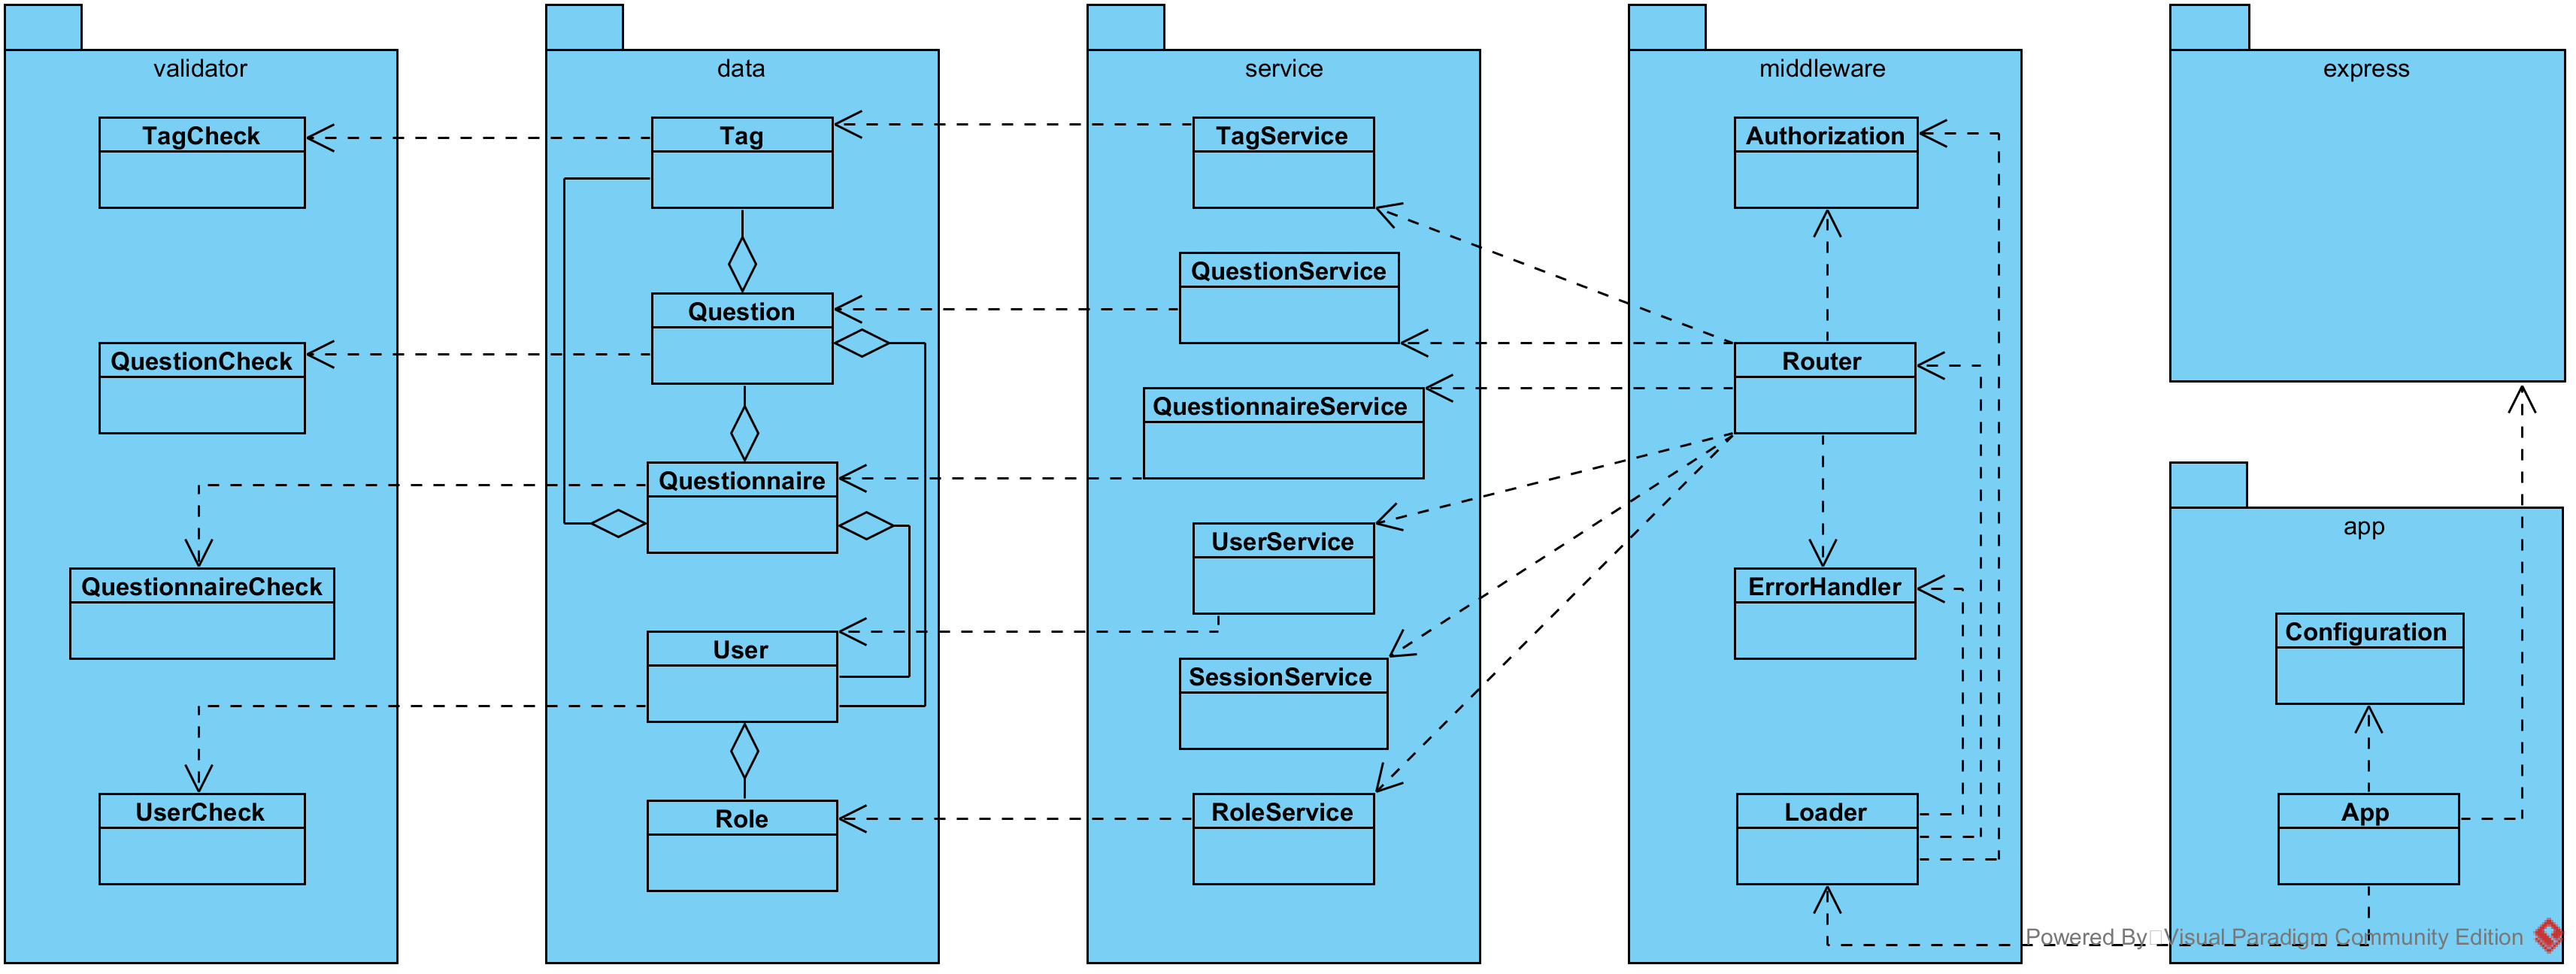
\includegraphics[scale=4, max width=\textwidth, max height=\myheight]{../img/diagrammiClassi/server.png}
		\caption{Diagramma package - server}
	\end{figure}
\end{center}\subsection{server::app}
Package che ha il compito di fornire i parametri di configurazione e avviare il web server di Quizzipedia\begin{center}
	\begin{figure}[H]
		\centering 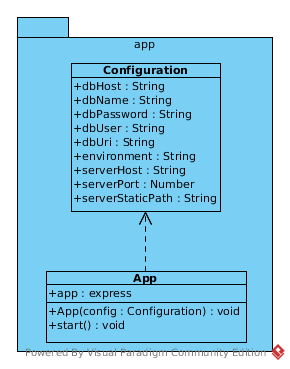
\includegraphics[scale=4, max width=\textwidth, max height=\myheight]{../img/diagrammiClassi/server/app.png}
		\caption{Diagramma package - server::app}
	\end{figure}
\end{center}\hypertarget{server::app::App}{}
\subsubsection[App]{server::app::App}
\begin{figure}[H]
	\centering
	\begin{tikzpicture}
	\umlclass{server::app::App} {+app : Express\\--config : Configuration}{+App(config : Configuration)\\+start() : void\\+config() : Express\\+getApp() : Express\\+setApp(app : Express) : void}
	\end{tikzpicture}
	\caption{Diagramma classe - server::app::App}
\end{figure}\begin{description}
\item[Descrizione] \hfill \\
Classe che si occupa di avviare il server e di invocare i middleware
\item[Utilizzo] \hfill \\
Viene utilizzata per avviare il server dell'applicazione
\item[Relazioni con altre classi] \hfill \\
\vspace{-7mm}
\begin{description}
	\item[\hyperlink{server::app::Configuration}{server::app::Configuration}] \hfill \\
	Relazione uscente, campo dati che rappresenta un riferimento a Configuration
\end{description}

\item[Attributi] \hfill \\
\vspace{-7mm}
\begin{itemize}
	\item app : Express $\rightarrow$ campo dati che rappresenta l'applicazione Express
	\item config : Configuration $\rightarrow$ campo dati che rappresenta un riferimento a Configuration
\end{itemize}

\item[Metodi] \hfill \\
\vspace{-7mm}
\begin{itemize}
	\item App(config : Configuration) $\rightarrow$ costruttore della classe\begin{itemize}
		\item config $\rightarrow$ configurazione per l'inizializzazione dell'applicazione
	\end{itemize}
	
	\item start() : void $\rightarrow$ metodo che avvia il server. Non ritorna il controllo fino a che il server è in funzione
	\item config() : Express $\rightarrow$ metodo che configura i parametri del server sulla base dell'oggetto di configurazione
	\item getApp() : Express $\rightarrow$ metodo getter
	\item setApp(app : Express) : void $\rightarrow$ metodo setter\begin{itemize}
		\item app $\rightarrow$ campo dati che rappresenta l'applicazione Express
	\end{itemize}
	
\end{itemize}

\end{description}

\vspace{0.5cm}
\hypertarget{server::app::Configuration}{}
\subsubsection[Configuration]{server::app::Configuration}
\begin{figure}[H]
	\centering
	\begin{tikzpicture}
	\umlclass{server::app::Configuration} {+environment : String\\+serverHost : String\\+serverPort : Number\\+serverStaticPath : String\\+dbHost : String\\+dbName : String\\+dbUser : String\\+dbPassword : String\\+dbUri : String\\+dbPort : number}{+getEnvironment() : String\\+getServerHost() : String\\+getServerPort() : Number\\+getServerStaticPath() : String\\+getDbHost() : String\\+getDbName() : String\\+getDbUser() : String\\+getDbPassword() : String\\+getDbUri() : String\\+getDbPort() : number\\+setEnvironment(environment : String) : void\\+setServerHost(serverHost : String) : void\\+setServerPort(serverPort : Number) : void\\+setServerStaticPath(serverStaticPath : String) : void\\+setDbHost(dbHost : String) : void\\+setDbName(dbName : String) : void\\+setDbUser(dbUser : String) : void\\+setDbPassword(dbPassword : String) : void\\+setDbUri(dbUri : String) : void\\+setDbPort(dbPort : number) : void}
	\end{tikzpicture}
	\caption{Diagramma classe - server::app::Configuration}
\end{figure}\begin{description}
\item[Descrizione] \hfill \\
Classe che contiene tutti i parametri di configurazione necessari al server e all'applicazione Quizzipedia per funzionare
\item[Utilizzo] \hfill \\
Viene utilizzata per definire le configurazioni dell'applicazione, passando un oggetto di questa classe al costruttore della classe App
\item[Relazioni con altre classi] \hfill \\
\vspace{-7mm}
\begin{description}
	\item[\hyperlink{server::app::App}{server::app::App}] \hfill \\
	Relazione entrante, campo dati che rappresenta un riferimento a Configuration
\end{description}

\item[Attributi] \hfill \\
\vspace{-7mm}
\begin{itemize}
	\item environment : String $\rightarrow$ variabile d'ambiente che informa se l'applicazione deve essere eseguita in modalità development o production
	\item serverHost : String $\rightarrow$ campo dati che identifica l'Indirizzo IP dell'host
	\item serverPort : Number $\rightarrow$ campo dati che identifica la porta su cui il server deve mettersi in ascolto
	\item serverStaticPath : String $\rightarrow$ campo dati che identifica il percorso della cartella che il server utilizza per fornire file statici
	\item dbHost : String $\rightarrow$ campo dati che identifica l'host del database
	\item dbName : String $\rightarrow$ campo dati che identifica il nome del database dell'applicazione
	\item dbUser : String $\rightarrow$ campo dati che identifica l'Username per connettersi al database
	\item dbPassword : String $\rightarrow$ campo dati che identifica la password per connettersi al database
	\item dbUri : String $\rightarrow$ campo dati che identifica l'Uri di connessione al database
	\item dbPort : number $\rightarrow$ campo dati che identifica la porta su cui il server di mongodb deve mettersi in ascolto
\end{itemize}

\item[Metodi] \hfill \\
\vspace{-7mm}
\begin{itemize}
	\item getEnvironment() : String $\rightarrow$ metodo getter
	\item getServerHost() : String $\rightarrow$ metodo getter
	\item getServerPort() : Number $\rightarrow$ metodo getter
	\item getServerStaticPath() : String $\rightarrow$ metodo getter
	\item getDbHost() : String $\rightarrow$ metodo getter
	\item getDbName() : String $\rightarrow$ metodo getter
	\item getDbUser() : String $\rightarrow$ metodo getter
	\item getDbPassword() : String $\rightarrow$ metodo getter
	\item getDbUri() : String $\rightarrow$ metodo getter
	\item getDbPort() : number $\rightarrow$ metodo getter
	\item setEnvironment(environment : String) : void $\rightarrow$ metodo setter\begin{itemize}
		\item environment $\rightarrow$ variabile d'ambiente che informa se l'applicazione deve essere eseguita in modalità development o production
	\end{itemize}
	
	\item setServerHost(serverHost : String) : void $\rightarrow$ metodo setter\begin{itemize}
		\item serverHost $\rightarrow$ campo dati che identifica l'Indirizzo IP dell'host
	\end{itemize}
	
	\item setServerPort(serverPort : Number) : void $\rightarrow$ metodo setter\begin{itemize}
		\item serverPort $\rightarrow$ campo dati che identifica la porta su cui il server deve mettersi in ascolto
	\end{itemize}
	
	\item setServerStaticPath(serverStaticPath : String) : void $\rightarrow$ metodo setter\begin{itemize}
		\item serverStaticPath $\rightarrow$ campo dati che identifica il percorso della cartella che il server utilizza per fornire file statici
	\end{itemize}
	
	\item setDbHost(dbHost : String) : void $\rightarrow$ metodo setter\begin{itemize}
		\item dbHost $\rightarrow$ campo dati che identifica l'host del database
	\end{itemize}
	
	\item setDbName(dbName : String) : void $\rightarrow$ metodo setter\begin{itemize}
		\item dbName $\rightarrow$ campo dati che identifica il nome del database dell'applicazione
	\end{itemize}
	
	\item setDbUser(dbUser : String) : void $\rightarrow$ metodo setter\begin{itemize}
		\item dbUser $\rightarrow$ campo dati che identifica l'Username per connettersi al database
	\end{itemize}
	
	\item setDbPassword(dbPassword : String) : void $\rightarrow$ metodo setter\begin{itemize}
		\item dbPassword $\rightarrow$ campo dati che identifica la password per connettersi al database
	\end{itemize}
	
	\item setDbUri(dbUri : String) : void $\rightarrow$ metodo setter\begin{itemize}
		\item dbUri $\rightarrow$ campo dati che identifica l'Uri di connessione al database
	\end{itemize}
	
	\item setDbPort(dbPort : number) : void $\rightarrow$ metodo setter\begin{itemize}
		\item dbPort $\rightarrow$ campo dati che identifica la porta su cui il server di mongodb deve mettersi in ascolto
	\end{itemize}
	
\end{itemize}

\end{description}

\vspace{0.5cm}
\subsection{server::express}
Express è un framework minimale, basato sul design pattern architetturale MVC per creare applicazioni web con Node.js. Express offre funzionalità che semplificano e aumentano le potenzialità di Node.js, fornendo una migliore implementazione del sistema di routing, incrementando
le funzioni di richiesta e risposta estendendole per una maggior flessibilità, integrando nuovi middleware, ed agevolando la realizzazione delle viste.
Express non limita l’utente nella scelta del linguaggio di templating, lo aiuta a gestire le route, le request e le view\begin{center}
	\begin{figure}[H]
		%\centering \includegraphics[scale=4, max width=\textwidth, max height=\myheight]{../img/diagrammiClassi/server/express.png}
		\caption{Diagramma package - server::express}
	\end{figure}
\end{center}\subsection{server::middleware}
Package che si occupa di ricevere richieste, richiamare il servizio adatto e restituire le risposte\begin{center}
	\begin{figure}[H]
		\centering 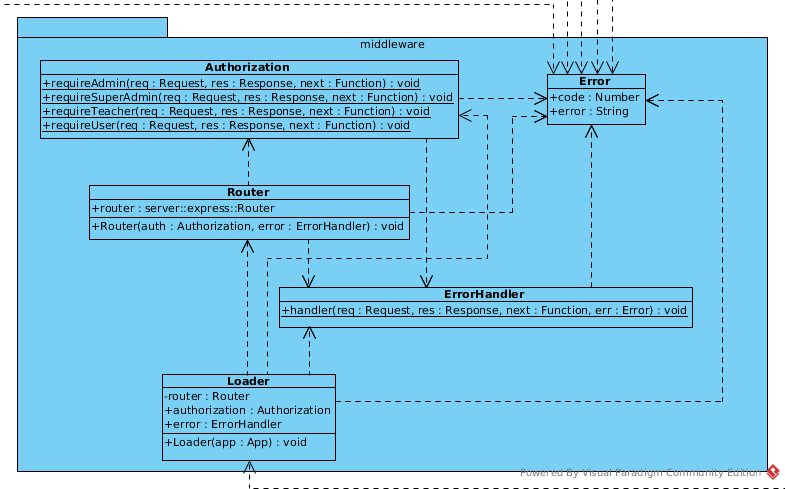
\includegraphics[scale=4, max width=\textwidth, max height=\myheight]{../img/diagrammiClassi/server/middleware.png}
		\caption{Diagramma package - server::middleware}
	\end{figure}
\end{center}\hypertarget{server::middleware::Router}{}
\subsubsection[Router]{server::middleware::Router}
\begin{figure}[H]
	\centering
	\begin{tikzpicture}
	\umlclass{server::middleware::Router} {--router : express.Router\\--sessionService : SessionService\\--userService : UserService\\--questionService : QuestionService\\--questionnaireService : QuestionnaireService\\--tagService : TagService\\--roleService : RoleService}{+Router(auth : Authorization, error : ErrorHandler)}
	\end{tikzpicture}
	\caption{Diagramma classe - server::middleware::Router}
\end{figure}\begin{description}
\item[Descrizione] \hfill \\
Classe che si occupa di instradare le richieste verso le relative richieste
\item[Utilizzo] \hfill \\
Si occupa di smistare la richiesta in base all’URI ricevuto e ad invocare l’opportuno servizio
\item[Relazioni con altre classi] \hfill \\
\vspace{-7mm}
\begin{description}
	\item[\hyperlink{server::service::SessionService}{server::service::SessionService}] \hfill \\
	Relazione uscente, campo dati che rappresenta un oggetto SessionService
	\item[\hyperlink{server::service::UserService}{server::service::UserService}] \hfill \\
	Relazione uscente, campo dati che rappresenta un oggetto UserService
	\item[\hyperlink{server::service::QuestionService}{server::service::QuestionService}] \hfill \\
	Relazione uscente, campo dati che rappresenta un oggetto QuestionService
	\item[\hyperlink{server::service::QuestionnaireService}{server::service::QuestionnaireService}] \hfill \\
	Relazione uscente, campo dati che rappresenta un oggetto QuestionnaireService
	\item[\hyperlink{server::service::TagService}{server::service::TagService}] \hfill \\
	Relazione uscente, campo dati che rappresenta un oggetto TagService
	\item[\hyperlink{server::service::RoleService}{server::service::RoleService}] \hfill \\
	Relazione uscente, campo dati che rappresenta un oggetto RoleService
	\item[\hyperlink{server::middleware::Loader}{server::middleware::Loader}] \hfill \\
	Relazione entrante, campo dati che rappresenta un riferimento al Middleware Router per gestire il reindirizzamento delle richieste
\end{description}

\item[Attributi] \hfill \\
\vspace{-7mm}
\begin{itemize}
	\item router : express.Router $\rightarrow$ campo dati che rappresenta un oggetto Router di Express
	\item sessionService : SessionService $\rightarrow$ campo dati che rappresenta un oggetto SessionService
	\item userService : UserService $\rightarrow$ campo dati che rappresenta un oggetto UserService
	\item questionService : QuestionService $\rightarrow$ campo dati che rappresenta un oggetto QuestionService
	\item questionnaireService : QuestionnaireService $\rightarrow$ campo dati che rappresenta un oggetto QuestionnaireService
	\item tagService : TagService $\rightarrow$ campo dati che rappresenta un oggetto TagService
	\item roleService : RoleService $\rightarrow$ campo dati che rappresenta un oggetto RoleService
\end{itemize}

\item[Metodi] \hfill \\
\vspace{-7mm}
\begin{itemize}
	\item Router(auth : Authorization, error : ErrorHandler) $\rightarrow$ costruttore della classe\begin{itemize}
		\item auth $\rightarrow$ istanza dell'oggetto Authorization
		\item error $\rightarrow$ istanza del gestore degli errori
	\end{itemize}
	
\end{itemize}

\end{description}

\vspace{0.5cm}
\hypertarget{server::middleware::Authorization}{}
\subsubsection[Authorization]{server::middleware::Authorization}
\begin{figure}[H]
	\centering
	\begin{tikzpicture}
	\umlclass{server::middleware::Authorization} {}{+requireRole(name : String) : Function\\+Authorization()}
	\end{tikzpicture}
	\caption{Diagramma classe - server::middleware::Authorization}
\end{figure}\begin{description}
\item[Descrizione] \hfill \\
Classe che si occupa dell’autorizzazione delle richieste
\item[Utilizzo] \hfill \\
Viene utilizzata per verificare i permessi dell'utente per ogni richiesta
\item[Relazioni con altre classi] \hfill \\
\vspace{-7mm}
\begin{description}
	\item[\hyperlink{server::middleware::Loader}{server::middleware::Loader}] \hfill \\
	Relazione entrante, campo dati che rappresenta un riferimento al Middleware Authorization, utilizzato per l'autorizzazione delle richieste
\end{description}

\item[Metodi] \hfill \\
\vspace{-7mm}
\begin{itemize}
	\item requireRole(name : String) : Function $\rightarrow$ metodo che verifica che l’utente autenticato sia almeno di ruolo specificato, richiamando il successivo middleware in caso affermativo, rispondendo con un errore altrimenti\begin{itemize}
		\item name $\rightarrow$ il nome del ruolo minimo richiesto
	\end{itemize}
	
	\item Authorization() $\rightarrow$ costruttore della classe
\end{itemize}

\end{description}

\vspace{0.5cm}
\hypertarget{server::middleware::Loader}{}
\subsubsection[Loader]{server::middleware::Loader}
\begin{figure}[H]
	\centering
	\begin{tikzpicture}
	\umlclass{server::middleware::Loader} {--authorization : Authorization\\--error : ErrorHandler\\--router : Router}{+Loader(app : App)}
	\end{tikzpicture}
	\caption{Diagramma classe - server::middleware::Loader}
\end{figure}\begin{description}
\item[Descrizione] \hfill \\
Classe utilizzata per istanziare tutti i middleware dell'applicazione
\item[Utilizzo] \hfill \\
Viene utilizzato per istanziare in modo nascosto all’applicazione tutti i middleware presenti nel componente server::middleware
\item[Relazioni con altre classi] \hfill \\
\vspace{-7mm}
\begin{description}
	\item[\hyperlink{server::middleware::Authorization}{server::middleware::Authorization}] \hfill \\
	Relazione uscente, campo dati che rappresenta un riferimento al Middleware Authorization, utilizzato per l'autorizzazione delle richieste
	\item[\hyperlink{server::middleware::Router}{server::middleware::Router}] \hfill \\
	Relazione uscente, campo dati che rappresenta un riferimento al Middleware Router per gestire il reindirizzamento delle richieste
	\item[\hyperlink{server::middleware::ErrorHandler}{server::middleware::ErrorHandler}] \hfill \\
	Relazione uscente, campo dati che rappresenta un riferimento al Middleware ErrorHandler, che si occupa di inoltrare le risposte d'errore al client
\end{description}

\item[Attributi] \hfill \\
\vspace{-7mm}
\begin{itemize}
	\item authorization : Authorization $\rightarrow$ campo dati che rappresenta un riferimento al Middleware Authorization, utilizzato per l'autorizzazione delle richieste
	\item error : ErrorHandler $\rightarrow$ campo dati che rappresenta un riferimento al Middleware ErrorHandler, che si occupa di inoltrare le risposte d'errore al client
	\item router : Router $\rightarrow$ campo dati che rappresenta un riferimento al Middleware Router per gestire il reindirizzamento delle richieste
\end{itemize}

\item[Metodi] \hfill \\
\vspace{-7mm}
\begin{itemize}
	\item Loader(app : App) $\rightarrow$ costruttore della classe\begin{itemize}
		\item app $\rightarrow$ applicazione su cui configurare i middleware
	\end{itemize}
	
\end{itemize}

\end{description}

\vspace{0.5cm}
\hypertarget{server::middleware::ErrorHandler}{}
\subsubsection[ErrorHandler]{server::middleware::ErrorHandler}
\begin{figure}[H]
	\centering
	\begin{tikzpicture}
	\umlclass{server::middleware::ErrorHandler} {}{+handler(req : Request, res : Response, next : Function, err : Error) : void\\+ErrorHandler()}
	\end{tikzpicture}
	\caption{Diagramma classe - server::middleware::ErrorHandler}
\end{figure}\begin{description}
\item[Descrizione] \hfill \\
Classe che gestisce gli errori generati nei controllers restituendo al client la risposta contenente il codice dell'errore verificatosi
\item[Utilizzo] \hfill \\
Questo middleware viene utilizzato per ultimo nella catena di gestione delle richieste di Express, in modo da gestire tutti gli errori generati precedentemente
\item[Relazioni con altre classi] \hfill \\
\vspace{-7mm}
\begin{description}
	\item[\hyperlink{server::middleware::Loader}{server::middleware::Loader}] \hfill \\
	Relazione entrante, campo dati che rappresenta un riferimento al Middleware ErrorHandler, che si occupa di inoltrare le risposte d'errore al client
\end{description}

\item[Metodi] \hfill \\
\vspace{-7mm}
\begin{itemize}
	\item handler(req : Request, res : Response, next : Function, err : Error) : void $\rightarrow$ metodo che gestisce l'errore generato dalla richiesta e da la relativa risposta con il codice dell'errore al client\begin{itemize}
		\item req $\rightarrow$ questo oggetto rappresenta la richiesta arrivata al server che il metodo deve gestire	
		\item res $\rightarrow$ questo oggetto rappresenta la risposta che il server dovrà inviare al termine dell'elaborazione	
		\item next $\rightarrow$ questo parametro rappresenta la callback che il metodo dovrà chiamare al termine dell’elaborazione	
		\item err $\rightarrow$ questo parametro rappresenta l'oggetto  dell'errore
	\end{itemize}
	
	\item ErrorHandler() $\rightarrow$ costruttore della classe
\end{itemize}

\end{description}

\vspace{0.5cm}
\subsection{server::data}
Package contenente le componenti che gestiscono i dati utilizzati dall'applicazione e l'interfacciamento con il database\begin{center}
	\begin{figure}[H]
		\centering 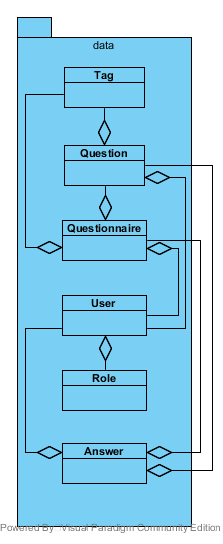
\includegraphics[scale=4, max width=\textwidth, max height=\myheight]{../img/diagrammiClassi/server/data.png}
		\caption{Diagramma package - server::data}
	\end{figure}
\end{center}\hypertarget{server::data::Tag}{}
\subsubsection[Tag]{server::data::Tag}
\begin{figure}[H]
	\centering
	\begin{tikzpicture}
	\umlclass{server::data::Tag} {+name : String\\+description : String}{+getName() : String\\+getDescription() : String\\+setName(name : String) : void\\+setDescription(description : String) : void}
	\end{tikzpicture}
	\caption{Diagramma classe - server::data::Tag}
\end{figure}\begin{description}
\item[Descrizione] \hfill \\
Classe che rappresenta una String contenente l'argomento da assegnare alle domande o ai questionari
\item[Relazioni con altre classi] \hfill \\
\vspace{-7mm}
\begin{description}
	\item[\hyperlink{server::data::Question}{server::data::Question}] \hfill \\
	Relazione entrante, campo dati che rappresenta l'insieme di riferimenti agli argomenti associati alla domanda
	\item[\hyperlink{server::data::Questionnaire}{server::data::Questionnaire}] \hfill \\
	Relazione entrante, campo dati che rappresenta l'insieme di riferimenti agli argomenti associati al questionario
\end{description}

\item[Attributi] \hfill \\
\vspace{-7mm}
\begin{itemize}
	\item name : String $\rightarrow$ campo dati contenente le parole dell'argomento separate da '-'
	\item description : String $\rightarrow$ campo dati che rappresenta una breve descrizione dell'attributo
\end{itemize}

\item[Metodi] \hfill \\
\vspace{-7mm}
\begin{itemize}
	\item getName() : String $\rightarrow$ metodo getter
	\item getDescription() : String $\rightarrow$ metodo getter
	\item setName(name : String) : void $\rightarrow$ metodo setter\begin{itemize}
		\item name $\rightarrow$ campo dati contenente le parole dell'argomento separate da '-'
	\end{itemize}
	
	\item setDescription(description : String) : void $\rightarrow$ metodo setter\begin{itemize}
		\item description $\rightarrow$ campo dati che rappresenta una breve descrizione dell'attributo
	\end{itemize}
	
\end{itemize}

\end{description}

\vspace{0.5cm}
\hypertarget{server::data::Questionnaire}{}
\subsubsection[Questionnaire]{server::data::Questionnaire}
\begin{figure}[H]
	\centering
	\begin{tikzpicture}
	\umlclass{server::data::Questionnaire} {+title : String\\+tags : Tag []\\+author : User\\+questions : Question []}{+getTitle() : String\\+getTags() : Tag []\\+getAuthor() : User\\+getQuestions() : Question []\\+setTitle(title : String) : void\\+setTags(tags : Tag []) : void\\+setAuthor(author : User) : void\\+setQuestions(questions : Question []) : void}
	\end{tikzpicture}
	\caption{Diagramma classe - server::data::Questionnaire}
\end{figure}\begin{description}
\item[Descrizione] \hfill \\
Classe che rappresenta un questionario
\item[Relazioni con altre classi] \hfill \\
\vspace{-7mm}
\begin{description}
	\item[\hyperlink{server::data::Question}{server::data::Question}] \hfill \\
	Relazione uscente, campo dati che rappresenta l'insieme di riferimenti alle domande del questionario
	\item[\hyperlink{server::data::Tag}{server::data::Tag}] \hfill \\
	Relazione uscente, campo dati che rappresenta l'insieme di riferimenti agli argomenti associati al questionario
	\item[\hyperlink{server::data::User}{server::data::User}] \hfill \\
	Relazione uscente, campo dati che rappresenta il riferimento all'autore del questionario
\end{description}

\item[Attributi] \hfill \\
\vspace{-7mm}
\begin{itemize}
	\item title : String $\rightarrow$ campo dati che rappresenta il titolo del questionario
	\item tags : Tag [] $\rightarrow$ campo dati che rappresenta l'insieme di riferimenti agli argomenti associati al questionario
	\item author : User $\rightarrow$ campo dati che rappresenta il riferimento all'autore del questionario
	\item questions : Question [] $\rightarrow$ campo dati che rappresenta l'insieme di riferimenti alle domande del questionario
\end{itemize}

\item[Metodi] \hfill \\
\vspace{-7mm}
\begin{itemize}
	\item getTitle() : String $\rightarrow$ metodo getter
	\item getTags() : Tag [] $\rightarrow$ metodo getter
	\item getAuthor() : User $\rightarrow$ metodo getter
	\item getQuestions() : Question [] $\rightarrow$ metodo getter
	\item setTitle(title : String) : void $\rightarrow$ metodo setter\begin{itemize}
		\item title $\rightarrow$ campo dati che rappresenta il titolo del questionario
	\end{itemize}
	
	\item setTags(tags : Tag []) : void $\rightarrow$ metodo setter\begin{itemize}
		\item tags $\rightarrow$ campo dati che rappresenta l'insieme di riferimenti agli argomenti associati al questionario
	\end{itemize}
	
	\item setAuthor(author : User) : void $\rightarrow$ metodo setter\begin{itemize}
		\item author $\rightarrow$ campo dati che rappresenta il riferimento all'autore del questionario
	\end{itemize}
	
	\item setQuestions(questions : Question []) : void $\rightarrow$ metodo setter\begin{itemize}
		\item questions $\rightarrow$ campo dati che rappresenta l'insieme di riferimenti alle domande del questionario
	\end{itemize}
	
\end{itemize}

\end{description}

\vspace{0.5cm}
\hypertarget{server::data::Question}{}
\subsubsection[Question]{server::data::Question}
\begin{figure}[H]
	\centering
	\begin{tikzpicture}
	\umlclass{server::data::Question} {+body : String\\+author : User\\+tags : Tag []}{+getBody() : String\\+getAuthor() : User\\+getTags() : Tag []\\+setBody(body : String) : void\\+setAuthor(author : User) : void\\+setTags(tags : Tag []) : void}
	\end{tikzpicture}
	\caption{Diagramma classe - server::data::Question}
\end{figure}\begin{description}
\item[Descrizione] \hfill \\
Classe base comune a tutti i tipi di domanda
\item[Relazioni con altre classi] \hfill \\
\vspace{-7mm}
\begin{description}
	\item[\hyperlink{server::data::Tag}{server::data::Tag}] \hfill \\
	Relazione uscente, campo dati che rappresenta l'insieme di riferimenti agli argomenti associati alla domanda
	\item[\hyperlink{server::data::User}{server::data::User}] \hfill \\
	Relazione uscente, campo dati che rappresenta il riferimento al docente che ha creato la domanda
	\item[\hyperlink{server::data::Questionnaire}{server::data::Questionnaire}] \hfill \\
	Relazione entrante, campo dati che rappresenta l'insieme di riferimenti alle domande del questionario
\end{description}

\item[Attributi] \hfill \\
\vspace{-7mm}
\begin{itemize}
	\item body : String $\rightarrow$ campo dati che rappresenta il QML del corpo della domanda
	\item author : User $\rightarrow$ campo dati che rappresenta il riferimento al docente che ha creato la domanda
	\item tags : Tag [] $\rightarrow$ campo dati che rappresenta l'insieme di riferimenti agli argomenti associati alla domanda
\end{itemize}

\item[Metodi] \hfill \\
\vspace{-7mm}
\begin{itemize}
	\item getBody() : String $\rightarrow$ metodo getter
	\item getAuthor() : User $\rightarrow$ metodo getter
	\item getTags() : Tag [] $\rightarrow$ metodo getter
	\item setBody(body : String) : void $\rightarrow$ metodo setter\begin{itemize}
		\item body $\rightarrow$ campo dati che rappresenta il QML del corpo della domanda
	\end{itemize}
	
	\item setAuthor(author : User) : void $\rightarrow$ metodo setter\begin{itemize}
		\item author $\rightarrow$ campo dati che rappresenta il riferimento al docente che ha creato la domanda
	\end{itemize}
	
	\item setTags(tags : Tag []) : void $\rightarrow$ metodo setter\begin{itemize}
		\item tags $\rightarrow$ campo dati che rappresenta l'insieme di riferimenti agli argomenti associati alla domanda
	\end{itemize}
	
\end{itemize}

\end{description}

\vspace{0.5cm}
\hypertarget{server::data::Role}{}
\subsubsection[Role]{server::data::Role}
\begin{figure}[H]
	\centering
	\begin{tikzpicture}
	\umlclass{server::data::Role} {+name : String}{+greaterThan(role : Role) : boolean\\+equalTo(role : Role) : boolean\\+getName() : String\\+setName(name : String) : void}
	\end{tikzpicture}
	\caption{Diagramma classe - server::data::Role}
\end{figure}\begin{description}
\item[Descrizione] \hfill \\
Classe che rappresenta un ruolo all'interno dell'applicazione
\item[Relazioni con altre classi] \hfill \\
\vspace{-7mm}
\begin{description}
	\item[\hyperlink{server::data::User}{server::data::User}] \hfill \\
	Relazione entrante, campo dati che rappresenta il riferimento al Role dell'utente nell'applicazione
\end{description}

\item[Attributi] \hfill \\
\vspace{-7mm}
\begin{itemize}
	\item name : String $\rightarrow$ campo dati che identifica la tipologia di utente
\end{itemize}

\item[Metodi] \hfill \\
\vspace{-7mm}
\begin{itemize}
	\item greaterThan(role : Role) : boolean $\rightarrow$ metodo che controlla se il ruolo è superiore (e non uguale) a quello passato\begin{itemize}
		\item role $\rightarrow$ l'altro ruolo da comparare
	\end{itemize}
	
	\item equalTo(role : Role) : boolean $\rightarrow$ metodo che controlla se il ruolo è uguale a quello passato\begin{itemize}
		\item role $\rightarrow$ l'altro ruolo da comparare
	\end{itemize}
	
	\item getName() : String $\rightarrow$ metodo getter
	\item setName(name : String) : void $\rightarrow$ metodo setter\begin{itemize}
		\item name $\rightarrow$ campo dati che identifica la tipologia di utente
	\end{itemize}
	
\end{itemize}

\end{description}

\vspace{0.5cm}
\hypertarget{server::data::User}{}
\subsubsection[User]{server::data::User}
\begin{figure}[H]
	\centering
	\begin{tikzpicture}
	\umlclass{server::data::User} {+fullName : String\\+role : Role\\+userName : String\\+password : String\\+isActive : boolean}{+hasPassword(rawPassword : String) : boolean\\+getFullName() : String\\+getRole() : Role\\+getUserName() : String\\+getPassword() : String\\+getIsActive() : boolean\\+setFullName(fullName : String) : void\\+setRole(role : Role) : void\\+setUserName(userName : String) : void\\+setPassword(password : String) : void\\+setIsActive(isActive : boolean) : void}
	\end{tikzpicture}
	\caption{Diagramma classe - server::data::User}
\end{figure}\begin{description}
\item[Descrizione] \hfill \\
Classe che rappresenta un utente dell'applicazione
\item[Relazioni con altre classi] \hfill \\
\vspace{-7mm}
\begin{description}
	\item[\hyperlink{server::data::Question}{server::data::Question}] \hfill \\
	Relazione entrante, campo dati che rappresenta il riferimento al docente che ha creato la domanda
	\item[\hyperlink{server::data::Questionnaire}{server::data::Questionnaire}] \hfill \\
	Relazione entrante, campo dati che rappresenta il riferimento all'autore del questionario
	\item[\hyperlink{server::data::Role}{server::data::Role}] \hfill \\
	Relazione uscente, campo dati che rappresenta il riferimento al Role dell'utente nell'applicazione
\end{description}

\item[Attributi] \hfill \\
\vspace{-7mm}
\begin{itemize}
	\item fullName : String $\rightarrow$ campo dati che rappresenta il nome e cognome dell'utente
	\item role : Role $\rightarrow$ campo dati che rappresenta il riferimento al Role dell'utente nell'applicazione
	\item userName : String $\rightarrow$ campo dati che rappresenta l'Username univoco con la quale, in combinazione con la password, l'utente accede al sistema
	\item password : String $\rightarrow$ campo dati contenente l'hash della password utilizzata per l'accesso
	\item isActive : boolean $\rightarrow$ campo dati che definisce se l'utente è attivo all'interno del sistema o se è stato disattivato
\end{itemize}

\item[Metodi] \hfill \\
\vspace{-7mm}
\begin{itemize}
	\item hasPassword(rawPassword : String) : boolean $\rightarrow$ metodo che controlla se la password dell'utente è uguale a quella passata\begin{itemize}
		\item rawPassword $\rightarrow$ la password in chiaro
	\end{itemize}
	
	\item getFullName() : String $\rightarrow$ metodo getter
	\item getRole() : Role $\rightarrow$ metodo getter
	\item getUserName() : String $\rightarrow$ metodo getter
	\item getPassword() : String $\rightarrow$ metodo getter
	\item getIsActive() : boolean $\rightarrow$ metodo getter
	\item setFullName(fullName : String) : void $\rightarrow$ metodo setter\begin{itemize}
		\item fullName $\rightarrow$ campo dati che rappresenta il nome e cognome dell'utente
	\end{itemize}
	
	\item setRole(role : Role) : void $\rightarrow$ metodo setter\begin{itemize}
		\item role $\rightarrow$ campo dati che rappresenta il riferimento al Role dell'utente nell'applicazione
	\end{itemize}
	
	\item setUserName(userName : String) : void $\rightarrow$ metodo setter\begin{itemize}
		\item userName $\rightarrow$ campo dati che rappresenta l'Username univoco con la quale, in combinazione con la password, l'utente accede al sistema
	\end{itemize}
	
	\item setPassword(password : String) : void $\rightarrow$ metodo setter\begin{itemize}
		\item password $\rightarrow$ campo dati contenente l'hash della password utilizzata per l'accesso
	\end{itemize}
	
	\item setIsActive(isActive : boolean) : void $\rightarrow$ metodo setter\begin{itemize}
		\item isActive $\rightarrow$ campo dati che definisce se l'utente è attivo all'interno del sistema o se è stato disattivato
	\end{itemize}
	
\end{itemize}

\end{description}

\vspace{0.5cm}
\subsection{server::service}
Package contenente le classi che implementano tutti i servizi offerti dall'applicazione lato server\begin{center}
	\begin{figure}[H]
		\centering 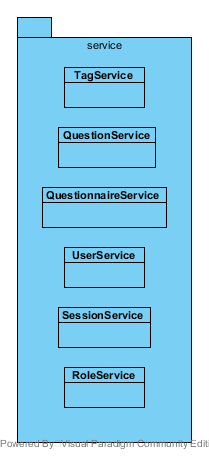
\includegraphics[scale=4, max width=\textwidth, max height=\myheight]{../img/diagrammiClassi/server/service.png}
		\caption{Diagramma package - server::service}
	\end{figure}
\end{center}\hypertarget{server::service::UserService}{}
\subsubsection[UserService]{server::service::UserService}
\begin{figure}[H]
	\centering
	\begin{tikzpicture}
	\umlclass{server::service::UserService} {}{+getByID(req : Request, res : Response, next : Function) : void\\+getMe(req : Request, res : Response, next : Function) : void\\+get(req : Request, res : Response, next : Function) : void\\+new(req : Request, res : Response, next : Function) : void\\+modify(req : Request, res : Response, next : Function) : void\\+delete(req : Request, res : Response, next : Function) : void\\+modifyMe(req : Request, res : Response, next : Function) : void\\+UserService()}
	\end{tikzpicture}
	\caption{Diagramma classe - server::service::UserService}
\end{figure}\begin{description}
\item[Descrizione] \hfill \\
Classe che si occupa della operazioni di inserimento, modifica e rimozione di account utenti.
\item[Utilizzo] \hfill \\
Fornisce i dati personali degli utenti a chi ne ha il permesso di accesso ed esegue operazioni di aggiunta, modifica, rimozione e cambio di ruolo per gli utenti del sistema.
\item[Relazioni con altre classi] \hfill \\
\vspace{-7mm}
\begin{description}
	\item[\hyperlink{server::middleware::Router}{server::middleware::Router}] \hfill \\
	Relazione entrante, campo dati che rappresenta un oggetto UserService
\end{description}

\item[Metodi] \hfill \\
\vspace{-7mm}
\begin{itemize}
	\item getByID(req : Request, res : Response, next : Function) : void $\rightarrow$ metodo che ritorna al client un Json contenente l'utente specifico identificato nella richiesta http\begin{itemize}
		\item req $\rightarrow$ questo oggetto rappresenta la richiesta arrivata al server che il metodo deve gestire
		\item res $\rightarrow$ questo oggetto rappresenta la risposta che il server dovrà inviare al termine dell'elaborazione
		\item next $\rightarrow$ questo parametro rappresenta la callback che il metodo dovrà chiamare al termine dell’elaborazione
	\end{itemize}
	
	\item getMe(req : Request, res : Response, next : Function) : void $\rightarrow$ metodo che restituisce al client un Json con i dati relativi all'utente loggato\begin{itemize}
		\item req $\rightarrow$ questo oggetto rappresenta la richiesta arrivata al server che il metodo deve gestire
		\item res $\rightarrow$ questo oggetto rappresenta la risposta che il server dovrà inviare al termine dell'elaborazione
		\item next $\rightarrow$ questo parametro rappresenta la callback che il metodo dovrà chiamare al termine dell’elaborazione
	\end{itemize}
	
	\item get(req : Request, res : Response, next : Function) : void $\rightarrow$ metodo che invia al client la lista degli utenti attraverso un Json\begin{itemize}
		\item req $\rightarrow$ questo oggetto rappresenta la richiesta arrivata al server che il metodo deve gestire
		\item res $\rightarrow$ questo oggetto rappresenta la risposta che il server dovrà inviare al termine dell'elaborazione
		\item next $\rightarrow$ questo parametro rappresenta la callback che il metodo dovrà chiamare al termine dell’elaborazione
	\end{itemize}
	
	\item new(req : Request, res : Response, next : Function) : void $\rightarrow$ metodo che aggiunge un nuovo utente al database\begin{itemize}
		\item req $\rightarrow$ questo oggetto rappresenta la richiesta arrivata al server che il metodo deve gestire
		\item res $\rightarrow$ questo oggetto rappresenta la risposta che il server dovrà inviare al termine dell'elaborazione
		\item next $\rightarrow$ questo parametro rappresenta la callback che il metodo dovrà chiamare al termine dell’elaborazione
	\end{itemize}
	
	\item modify(req : Request, res : Response, next : Function) : void $\rightarrow$ metodo che modifica i dati dell'utente specificato nella richiesta http\begin{itemize}
		\item req $\rightarrow$ questo oggetto rappresenta la richiesta arrivata al server che il metodo deve gestire
		\item res $\rightarrow$ questo oggetto rappresenta la risposta che il server dovrà inviare al termine dell'elaborazione
		\item next $\rightarrow$ questo parametro rappresenta la callback che il metodo dovrà chiamare al termine dell’elaborazione
	\end{itemize}
	
	\item delete(req : Request, res : Response, next : Function) : void $\rightarrow$ metodo che elimina un utente dal database\begin{itemize}
		\item req $\rightarrow$ questo oggetto rappresenta la richiesta arrivata al server che il metodo deve gestire
		\item res $\rightarrow$ questo oggetto rappresenta la risposta che il server dovrà inviare al termine dell'elaborazione
		\item next $\rightarrow$ questo parametro rappresenta la callback che il metodo dovrà chiamare al termine dell’elaborazione
	\end{itemize}
	
	\item modifyMe(req : Request, res : Response, next : Function) : void $\rightarrow$ metodo che modifica i dati dell'utente connesso al sistema se presente\begin{itemize}
		\item req $\rightarrow$ questo oggetto rappresenta la richiesta arrivata al server che il metodo deve gestire
		\item res $\rightarrow$ questo oggetto rappresenta la risposta che il server dovrà inviare al termine dell'elaborazione
		\item next $\rightarrow$ questo parametro rappresenta la callback che il metodo dovrà chiamare al termine dell’elaborazione
	\end{itemize}
	
	\item UserService() $\rightarrow$ costruttore della classe
\end{itemize}

\end{description}

\vspace{0.5cm}
\hypertarget{server::service::QuestionnaireService}{}
\subsubsection[QuestionnaireService]{server::service::QuestionnaireService}
\begin{figure}[H]
	\centering
	\begin{tikzpicture}
	\umlclass{server::service::QuestionnaireService} {}{+getByID(req : Request, res : Response, next : Function) : void\\+get(req : Request, res : Response, next : Function) : void\\+new(req : Request, res : Response, next : Function) : void\\+modify(req : Request, res : Response, next : Function) : void\\+delete(req : Request, res : Response, next : Function) : void\\+QuestionnaireService()}
	\end{tikzpicture}
	\caption{Diagramma classe - server::service::QuestionnaireService}
\end{figure}\begin{description}
\item[Descrizione] \hfill \\
Classe che si occupa di gestire questionari. È uno dei componenti product del Design Pattern Abstract Factory
\item[Utilizzo] \hfill \\
Offre metodi per restituire questionari. Permette inoltre ad un docente di effettuare l'inserimento, la modifica, l'eliminazione di questionari
\item[Relazioni con altre classi] \hfill \\
\vspace{-7mm}
\begin{description}
	\item[\hyperlink{server::middleware::Router}{server::middleware::Router}] \hfill \\
	Relazione entrante, campo dati che rappresenta un oggetto QuestionnaireService
\end{description}

\item[Metodi] \hfill \\
\vspace{-7mm}
\begin{itemize}
	\item getByID(req : Request, res : Response, next : Function) : void $\rightarrow$ metodo che ritorna al client un Json contenente il questionario specifico richiesto identificato nella richiesta http\begin{itemize}
		\item req $\rightarrow$ questo oggetto rappresenta la richiesta arrivata al server che il metodo deve gestire
		\item res $\rightarrow$ questo oggetto rappresenta la risposta che il server dovrà inviare al termine dell'elaborazione
		\item next $\rightarrow$ questo parametro rappresenta la callback che il metodo dovrà chiamare al termine dell’elaborazione
	\end{itemize}
	
	\item get(req : Request, res : Response, next : Function) : void $\rightarrow$ metodo che invia al client una lista di questionari attraverso un Json\begin{itemize}
		\item req $\rightarrow$ questo oggetto rappresenta la richiesta arrivata al server che il metodo deve gestire
		\item res $\rightarrow$ questo oggetto rappresenta la risposta che il server dovrà inviare al termine dell'elaborazione
		\item next $\rightarrow$ questo parametro rappresenta la callback che il metodo dovrà chiamare al termine dell’elaborazione
	\end{itemize}
	
	\item new(req : Request, res : Response, next : Function) : void $\rightarrow$ metodo che aggiunge un nuovo questionario al database\begin{itemize}
		\item req $\rightarrow$ questo oggetto rappresenta la richiesta arrivata al server che il metodo deve gestire
		\item res $\rightarrow$ questo oggetto rappresenta la risposta che il server dovrà inviare al termine dell'elaborazione
		\item next $\rightarrow$ questo parametro rappresenta la callback che il metodo dovrà chiamare al termine dell’elaborazione
	\end{itemize}
	
	\item modify(req : Request, res : Response, next : Function) : void $\rightarrow$ metodo che modifica un questionario specificato nella richiesta http\begin{itemize}
		\item req $\rightarrow$ questo oggetto rappresenta la richiesta arrivata al server che il metodo deve gestire
		\item res $\rightarrow$ questo oggetto rappresenta la risposta che il server dovrà inviare al termine dell'elaborazione
		\item next $\rightarrow$ questo parametro rappresenta la callback che il metodo dovrà chiamare al termine dell’elaborazione
	\end{itemize}
	
	\item delete(req : Request, res : Response, next : Function) : void $\rightarrow$ metodo che cancella un questionario specifico dal database\begin{itemize}
		\item req $\rightarrow$ questo oggetto rappresenta la richiesta arrivata al server che il metodo deve gestire
		\item res $\rightarrow$ questo oggetto rappresenta la risposta che il server dovrà inviare al termine dell'elaborazione
		\item next $\rightarrow$ questo parametro rappresenta la callback che il metodo dovrà chiamare al termine dell’elaborazione
	\end{itemize}
	
	\item QuestionnaireService() $\rightarrow$ costruttore della classe
\end{itemize}

\end{description}

\vspace{0.5cm}
\hypertarget{server::service::QuestionService}{}
\subsubsection[QuestionService]{server::service::QuestionService}
\begin{figure}[H]
	\centering
	\begin{tikzpicture}
	\umlclass{server::service::QuestionService} {}{+get(req : Request, res : Response, next : Function) : void\\+getByID(req : Request, res : Response, next : Function) : void\\+new(req : Request, res : Response, next : Function) : void\\+modify(req : Request, res : Response, next : Function) : void\\+delete(req : Request, res : Response, next : Function) : void\\+QuestionService()}
	\end{tikzpicture}
	\caption{Diagramma classe - server::service::QuestionService}
\end{figure}\begin{description}
\item[Descrizione] \hfill \\
Classe che si occupa di gestire domande. È uno dei componenti product del Design Pattern Abstract Factory
\item[Utilizzo] \hfill \\
Offre metodi per restituire le domande. Permette inoltre ad un docente di effettuare l'inserimento, la modifica, l'eliminazione di domande
\item[Relazioni con altre classi] \hfill \\
\vspace{-7mm}
\begin{description}
	\item[\hyperlink{server::middleware::Router}{server::middleware::Router}] \hfill \\
	Relazione entrante, campo dati che rappresenta un oggetto QuestionService
\end{description}

\item[Metodi] \hfill \\
\vspace{-7mm}
\begin{itemize}
	\item get(req : Request, res : Response, next : Function) : void $\rightarrow$ metodo che invia al client una lista di domande attraverso un Json\begin{itemize}
		\item req $\rightarrow$ questo oggetto rappresenta la richiesta arrivata al server che il metodo deve gestire
		\item res $\rightarrow$ questo oggetto rappresenta la risposta che il server dovrà inviare al termine dell'elaborazione
		\item next $\rightarrow$ questo parametro rappresenta la callback che il metodo dovrà chiamare al termine dell’elaborazione
	\end{itemize}
	
	\item getByID(req : Request, res : Response, next : Function) : void $\rightarrow$ metodo che ritorna al client un Json contenente la domanda specifica identificata nella richiesta http\begin{itemize}
		\item req $\rightarrow$ questo oggetto rappresenta la richiesta arrivata al server che il metodo deve gestire
		\item res $\rightarrow$ questo oggetto rappresenta la risposta che il server dovrà inviare al termine dell'elaborazione
		\item next $\rightarrow$ questo parametro rappresenta la callback che il metodo dovrà chiamare al termine dell’elaborazione
	\end{itemize}
	
	\item new(req : Request, res : Response, next : Function) : void $\rightarrow$ metodo che aggiunge una nuova domanda al database\begin{itemize}
		\item req $\rightarrow$ questo oggetto rappresenta la richiesta arrivata al server che il metodo deve gestire
		\item res $\rightarrow$ questo oggetto rappresenta la risposta che il server dovrà inviare al termine dell'elaborazione
		\item next $\rightarrow$ questo parametro rappresenta la callback che il metodo dovrà chiamare al termine dell’elaborazione
	\end{itemize}
	
	\item modify(req : Request, res : Response, next : Function) : void $\rightarrow$ metodo che modifica una domanda specificato nella richiesta http\begin{itemize}
		\item req $\rightarrow$ questo oggetto rappresenta la richiesta arrivata al server che il metodo deve gestire
		\item res $\rightarrow$ questo oggetto rappresenta la risposta che il server dovrà inviare al termine dell'elaborazione
		\item next $\rightarrow$ questo parametro rappresenta la callback che il metodo dovrà chiamare al termine dell’elaborazione
	\end{itemize}
	
	\item delete(req : Request, res : Response, next : Function) : void $\rightarrow$ metodo che elimina una domanda selezionata dal database\begin{itemize}
		\item req $\rightarrow$ questo oggetto rappresenta la richiesta arrivata al server che il metodo deve gestire
		\item res $\rightarrow$ questo oggetto rappresenta la risposta che il server dovrà inviare al termine dell'elaborazione
		\item next $\rightarrow$ questo parametro rappresenta la callback che il metodo dovrà chiamare al termine dell’elaborazione
	\end{itemize}
	
	\item QuestionService() $\rightarrow$ costruttore della classe
\end{itemize}

\end{description}

\vspace{0.5cm}
\hypertarget{server::service::TagService}{}
\subsubsection[TagService]{server::service::TagService}
\begin{figure}[H]
	\centering
	\begin{tikzpicture}
	\umlclass{server::service::TagService} {}{+get(req : Request, res : Response, next : Function) : void\\+getByID(req : Request, res : Response, next : Function) : void\\+new(req : Request, res : Response, next : Function) : void\\+modify(req : Request, res : Response, next : Function) : void\\+delete(req : Request, res : Response, next : Function) : void\\+TagService()}
	\end{tikzpicture}
	\caption{Diagramma classe - server::service::TagService}
\end{figure}\begin{description}
\item[Descrizione] \hfill \\
Classe che si occupa di gestire gli argomenti. È uno dei componenti product del Design Pattern Abstract Factory
\item[Utilizzo] \hfill \\
Offre metodi per restituire gli argomenti presenti. Permette inoltre ad un docente di effettuare l'inserimento, la modifica, l'eliminazione di argomenti
\item[Relazioni con altre classi] \hfill \\
\vspace{-7mm}
\begin{description}
	\item[\hyperlink{server::middleware::Router}{server::middleware::Router}] \hfill \\
	Relazione entrante, campo dati che rappresenta un oggetto TagService
\end{description}

\item[Metodi] \hfill \\
\vspace{-7mm}
\begin{itemize}
	\item get(req : Request, res : Response, next : Function) : void $\rightarrow$ metodo che invia al client la lista degli argomenti attraverso un Json\begin{itemize}
		\item req $\rightarrow$ questo oggetto rappresenta la richiesta arrivata al server che il metodo deve gestire
		\item res $\rightarrow$ questo oggetto rappresenta la risposta che il server dovrà inviare al termine dell'elaborazione
		\item next $\rightarrow$ questo parametro rappresenta la callback che il metodo dovrà chiamare al termine dell’elaborazione
	\end{itemize}
	
	\item getByID(req : Request, res : Response, next : Function) : void $\rightarrow$ metodo che ritorna al client un Json contenente l'argomento specifico identificato nella richiesta http\begin{itemize}
		\item req $\rightarrow$ questo oggetto rappresenta la richiesta arrivata al server che il metodo deve gestire
		\item res $\rightarrow$ questo oggetto rappresenta la risposta che il server dovrà inviare al termine dell'elaborazione
		\item next $\rightarrow$ questo parametro rappresenta la callback che il metodo dovrà chiamare al termine dell’elaborazione
	\end{itemize}
	
	\item new(req : Request, res : Response, next : Function) : void $\rightarrow$ metodo che aggiunge un nuovo argomento al database\begin{itemize}
		\item req $\rightarrow$ questo oggetto rappresenta la richiesta arrivata al server che il metodo deve gestire
		\item res $\rightarrow$ questo oggetto rappresenta la risposta che il server dovrà inviare al termine dell'elaborazione
		\item next $\rightarrow$ questo parametro rappresenta la callback che il metodo dovrà chiamare al termine dell’elaborazione
	\end{itemize}
	
	\item modify(req : Request, res : Response, next : Function) : void $\rightarrow$ metodo che modifica un argomento specificato nella richiesta http\begin{itemize}
		\item req $\rightarrow$ questo oggetto rappresenta la richiesta arrivata al server che il metodo deve gestire
		\item res $\rightarrow$ questo oggetto rappresenta la risposta che il server dovrà inviare al termine dell'elaborazione
		\item next $\rightarrow$ questo parametro rappresenta la callback che il metodo dovrà chiamare al termine dell’elaborazione
	\end{itemize}
	
	\item delete(req : Request, res : Response, next : Function) : void $\rightarrow$ metodo che elimina un argomento specifico dal database\begin{itemize}
		\item req $\rightarrow$ questo oggetto rappresenta la richiesta arrivata al server che il metodo deve gestire
		\item res $\rightarrow$ questo oggetto rappresenta la risposta che il server dovrà inviare al termine dell'elaborazione
		\item next $\rightarrow$ questo parametro rappresenta la callback che il metodo dovrà chiamare al termine dell’elaborazione
	\end{itemize}
	
	\item TagService() $\rightarrow$ costruttore della classe
\end{itemize}

\end{description}

\vspace{0.5cm}
\hypertarget{server::service::SessionService}{}
\subsubsection[SessionService]{server::service::SessionService}
\begin{figure}[H]
	\centering
	\begin{tikzpicture}
	\umlclass{server::service::SessionService} {}{+new(req : Request, res : Response, next : Function) : void\\+delete(req : Request, res : Response, next : Function) : void\\+SessionService()}
	\end{tikzpicture}
	\caption{Diagramma classe - server::service::SessionService}
\end{figure}\begin{description}
\item[Descrizione] \hfill \\
Classe che si occupa della gestione della sessione dell'utente
\item[Utilizzo] \hfill \\
Viene utilizzata per gestire il login e logout dell'utente
\item[Relazioni con altre classi] \hfill \\
\vspace{-7mm}
\begin{description}
	\item[\hyperlink{server::middleware::Router}{server::middleware::Router}] \hfill \\
	Relazione entrante, campo dati che rappresenta un oggetto SessionService
\end{description}

\item[Metodi] \hfill \\
\vspace{-7mm}
\begin{itemize}
	\item new(req : Request, res : Response, next : Function) : void $\rightarrow$ metodo che crea una sessione con una volta che l'utente effettua l'accesso all'applicazione\begin{itemize}
		\item req $\rightarrow$ questo oggetto rappresenta la richiesta arrivata al server che il metodo deve gestire
		\item res $\rightarrow$ questo oggetto rappresenta la risposta che il server dovrà inviare al termine dell'elaborazione
		\item next $\rightarrow$ questo parametro rappresenta la callback che il metodo dovrà chiamare al termine dell’elaborazione
	\end{itemize}
	
	\item delete(req : Request, res : Response, next : Function) : void $\rightarrow$ metodo che elimina la sessione dell'utente dal database\begin{itemize}
		\item req $\rightarrow$ questo oggetto rappresenta la richiesta arrivata al server che il metodo deve gestire
		\item res $\rightarrow$ questo oggetto rappresenta la risposta che il server dovrà inviare al termine dell'elaborazione
		\item next $\rightarrow$ questo parametro rappresenta la callback che il metodo dovrà chiamare al termine dell’elaborazione
	\end{itemize}
	
	\item SessionService() $\rightarrow$ costruttore della classe
\end{itemize}

\end{description}

\vspace{0.5cm}
\hypertarget{server::service::RoleService}{}
\subsubsection[RoleService]{server::service::RoleService}
\begin{figure}[H]
	\centering
	\begin{tikzpicture}
	\umlclass{server::service::RoleService} {}{+get(req : Request, res : Response, next : Function) : void\\+getByID(req : Request, res : Response, next : Function) : void\\+RoleService()}
	\end{tikzpicture}
	\caption{Diagramma classe - server::service::RoleService}
\end{figure}\begin{description}
\item[Descrizione] \hfill \\
Classe che rappresenta il servizio per la lettura dei ruoli utente
\item[Utilizzo] \hfill \\
Viene utilizzata per fornire un punto d'accesso per l'elenco di tutti i ruoli dell'applicazione e la lettura di un singolo ruolo
\item[Relazioni con altre classi] \hfill \\
\vspace{-7mm}
\begin{description}
	\item[\hyperlink{server::middleware::Router}{server::middleware::Router}] \hfill \\
	Relazione entrante, campo dati che rappresenta un oggetto RoleService
\end{description}

\item[Metodi] \hfill \\
\vspace{-7mm}
\begin{itemize}
	\item get(req : Request, res : Response, next : Function) : void $\rightarrow$ metodo che invia al client la lista di tutti i ruoli assumibili dagli utenti dell'applicazione attraverso un Json\begin{itemize}
		\item req $\rightarrow$ questo oggetto rappresenta la richiesta arrivata al server che il metodo deve gestire
		\item res $\rightarrow$ questo oggetto rappresenta la risposta che il server dovrà inviare al termine dell'elaborazione
		\item next $\rightarrow$ questo parametro rappresenta la callback che il metodo dovrà chiamare al termine dell’elaborazione
	\end{itemize}
	
	\item getByID(req : Request, res : Response, next : Function) : void $\rightarrow$ metodo che ritorna al client un Json contenente il ruolo specificato nella richiesta http\begin{itemize}
		\item req $\rightarrow$ questo oggetto rappresenta la richiesta arrivata al server che il metodo deve gestire
		\item res $\rightarrow$ questo oggetto rappresenta la risposta che il server dovrà inviare al termine dell'elaborazione
		\item next $\rightarrow$ questo parametro rappresenta la callback che il metodo dovrà chiamare al termine dell’elaborazione
	\end{itemize}
	
	\item RoleService() $\rightarrow$ costruttore della classe
\end{itemize}

\end{description}

\vspace{0.5cm}
\subsection{server::validator}
Package contenente tutte le classi "validator" che hanno il compito di controllare che alcuni campi di alcuni model siano validi; esempi includono la password dell'utente, la lunghezza del nome utente o il QML di una domanda\begin{center}
	\begin{figure}[H]
		\centering 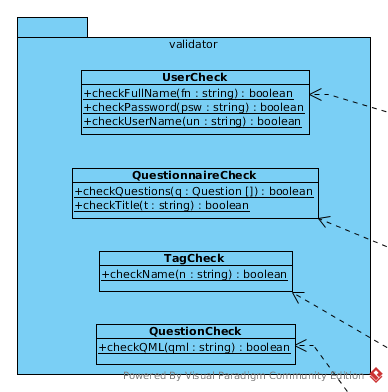
\includegraphics[scale=4, max width=\textwidth, max height=\myheight]{../img/diagrammiClassi/server/validator.png}
		\caption{Diagramma package - server::validator}
	\end{figure}
\end{center}\hypertarget{server::validator::UserCheck}{}
\subsubsection[UserCheck]{server::validator::UserCheck}
\begin{figure}[H]
	\centering
	\begin{tikzpicture}
	\umlclass{server::validator::UserCheck} {}{+checkFullName(fullName : String) : boolean\\+checkPassword(psw : String) : boolean\\+checkUserName(userName : String) : boolean\\+UserCheck()}
	\end{tikzpicture}
	\caption{Diagramma classe - server::validator::UserCheck}
\end{figure}\begin{description}
\item[Descrizione] \hfill \\
Classe contenente tutte le funzioni di controllo della validità dei campi del model User
\item[Utilizzo] \hfill \\
Viene utilizzata dai service per effettuare controlli sul model User
\item[Metodi] \hfill \\
\vspace{-7mm}
\begin{itemize}
	\item checkFullName(fullName : String) : boolean $\rightarrow$ metodo che controlla che il nome completo passato contenga almeno 2 caratteri\begin{itemize}
		\item fullName $\rightarrow$ il nome completo da controllare
	\end{itemize}
	
	\item checkPassword(psw : String) : boolean $\rightarrow$ metodo che controlla che la password passata contenga almeno 6 caratteri\begin{itemize}
		\item psw $\rightarrow$ la password, ovviamente in chiaro (non l'hash), da controllare
	\end{itemize}
	
	\item checkUserName(userName : String) : boolean $\rightarrow$ metodo che controlla che l'username passato contenga almeno 6 caratteri\begin{itemize}
		\item userName $\rightarrow$ l'username da controllare
	\end{itemize}
	
	\item UserCheck() $\rightarrow$ costruttore della classe
\end{itemize}

\end{description}

\vspace{0.5cm}
\hypertarget{server::validator::QuestionnaireCheck}{}
\subsubsection[QuestionnaireCheck]{server::validator::QuestionnaireCheck}
\begin{figure}[H]
	\centering
	\begin{tikzpicture}
	\umlclass{server::validator::QuestionnaireCheck} {}{+checkQuestions(questions : Question []) : boolean\\+checkTitle(title : String) : boolean\\+checkTags(tags : Tag []) : boolean\\+QuestionnaireCheck()}
	\end{tikzpicture}
	\caption{Diagramma classe - server::validator::QuestionnaireCheck}
\end{figure}\begin{description}
\item[Descrizione] \hfill \\
Classe contenente tutte le funzioni di controllo della validità dei campi del model Questionnaire
\item[Utilizzo] \hfill \\
Viene utilizzata dai service per effettuare controlli sul model User
\item[Metodi] \hfill \\
\vspace{-7mm}
\begin{itemize}
	\item checkQuestions(questions : Question []) : boolean $\rightarrow$ metodo che controlla che la lista/array di domande passate non sia vuota e che non contenga domande duplicate\begin{itemize}
		\item questions $\rightarrow$ l'elenco delle domande del questionario
	\end{itemize}
	
	\item checkTitle(title : String) : boolean $\rightarrow$ metodo che controlla che il titolo del questionario non sia vuoto\begin{itemize}
		\item title $\rightarrow$ il titolo del questionario da controllare
	\end{itemize}
	
	\item checkTags(tags : Tag []) : boolean $\rightarrow$ metodo che controlla che la lista/array di argomenti passati non sia vuota\begin{itemize}
		\item tags $\rightarrow$ elenco degli argomenti	
	\end{itemize}
	
	\item QuestionnaireCheck() $\rightarrow$ costruttore della classe
\end{itemize}

\end{description}

\vspace{0.5cm}
\hypertarget{server::validator::TagCheck}{}
\subsubsection[TagCheck]{server::validator::TagCheck}
\begin{figure}[H]
	\centering
	\begin{tikzpicture}
	\umlclass{server::validator::TagCheck} {}{+checkName(name : String) : boolean\\+TagCheck()}
	\end{tikzpicture}
	\caption{Diagramma classe - server::validator::TagCheck}
\end{figure}\begin{description}
\item[Descrizione] \hfill \\
Classe contenente tutte le funzioni di controllo della validità dei campi del model Tag
\item[Utilizzo] \hfill \\
Viene utilizzata dai service per effettuare controlli sul model Tag
\item[Metodi] \hfill \\
\vspace{-7mm}
\begin{itemize}
	\item checkName(name : String) : boolean $\rightarrow$ metodo che controlla che il nome dell'argomento non sia vuoto\begin{itemize}
		\item name $\rightarrow$ il nome dell'argomento da controllare
	\end{itemize}
	
	\item TagCheck() $\rightarrow$ costruttore della classe
\end{itemize}

\end{description}

\vspace{0.5cm}
\hypertarget{server::validator::QuestionCheck}{}
\subsubsection[QuestionCheck]{server::validator::QuestionCheck}
\begin{figure}[H]
	\centering
	\begin{tikzpicture}
	\umlclass{server::validator::QuestionCheck} {}{+checkQML(qml : String) : boolean\\+checkTags(tags : Tag []) : boolean\\+QuestionCheck()}
	\end{tikzpicture}
	\caption{Diagramma classe - server::validator::QuestionCheck}
\end{figure}\begin{description}
\item[Descrizione] \hfill \\
Classe contenente tutte le funzioni di controllo della validità dei campi del model Question
\item[Utilizzo] \hfill \\
Viene utilizzata dai service per effettuare controlli sul model Question
\item[Metodi] \hfill \\
\vspace{-7mm}
\begin{itemize}
	\item checkQML(qml : String) : boolean $\rightarrow$ metodo che controlla che la stringa di QML (generalmente quella dell'attributo body del model Question) sia QML valido\begin{itemize}
		\item qml $\rightarrow$ la stringa in formato QML da controllare
	\end{itemize}
	
	\item checkTags(tags : Tag []) : boolean $\rightarrow$ metodo che controlla che la lista/array di argomenti passati non sia vuota\begin{itemize}
		\item tags $\rightarrow$ elenco degli argomenti
	\end{itemize}
	
	\item QuestionCheck() $\rightarrow$ costruttore della classe
\end{itemize}

\end{description}

\newpage

%Specifica componenti client
\section{Specifica componenti client}
È il package che racchiude tutte le parti del front-end. Contiene le componenti che vengono eseguite nel browser da un qualsiasi utente, fornendo loro un’interfaccia grafica per interagire con il sistema.
Viene fornito di seguito il diagramma dei \mgls{package} ad alto livello.
\begin{center}
	\begin{figure}[H]
		\centering 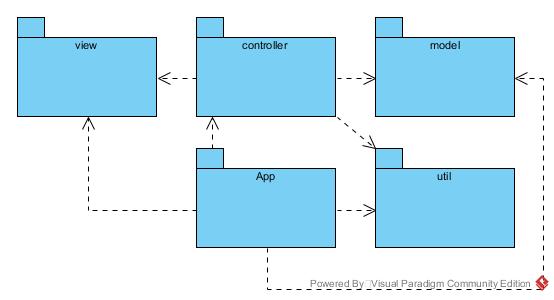
\includegraphics[scale=4, max width=\textwidth, max height=\myheight]{../img/diagrammiClassi/architetturaClient.png}
		\caption{Diagramma package - client}
	\end{figure}
\end{center}

Al fine di rendere il diagramma delle classi del client più leggibile si è deciso di dividerlo, quindi di seguito si può vedere il diagramma delle classi, con le relative relazione, di \texttt{view}, \texttt{controller} e \texttt{util}.
\begin{center}
	\begin{figure}[H]
		\centering 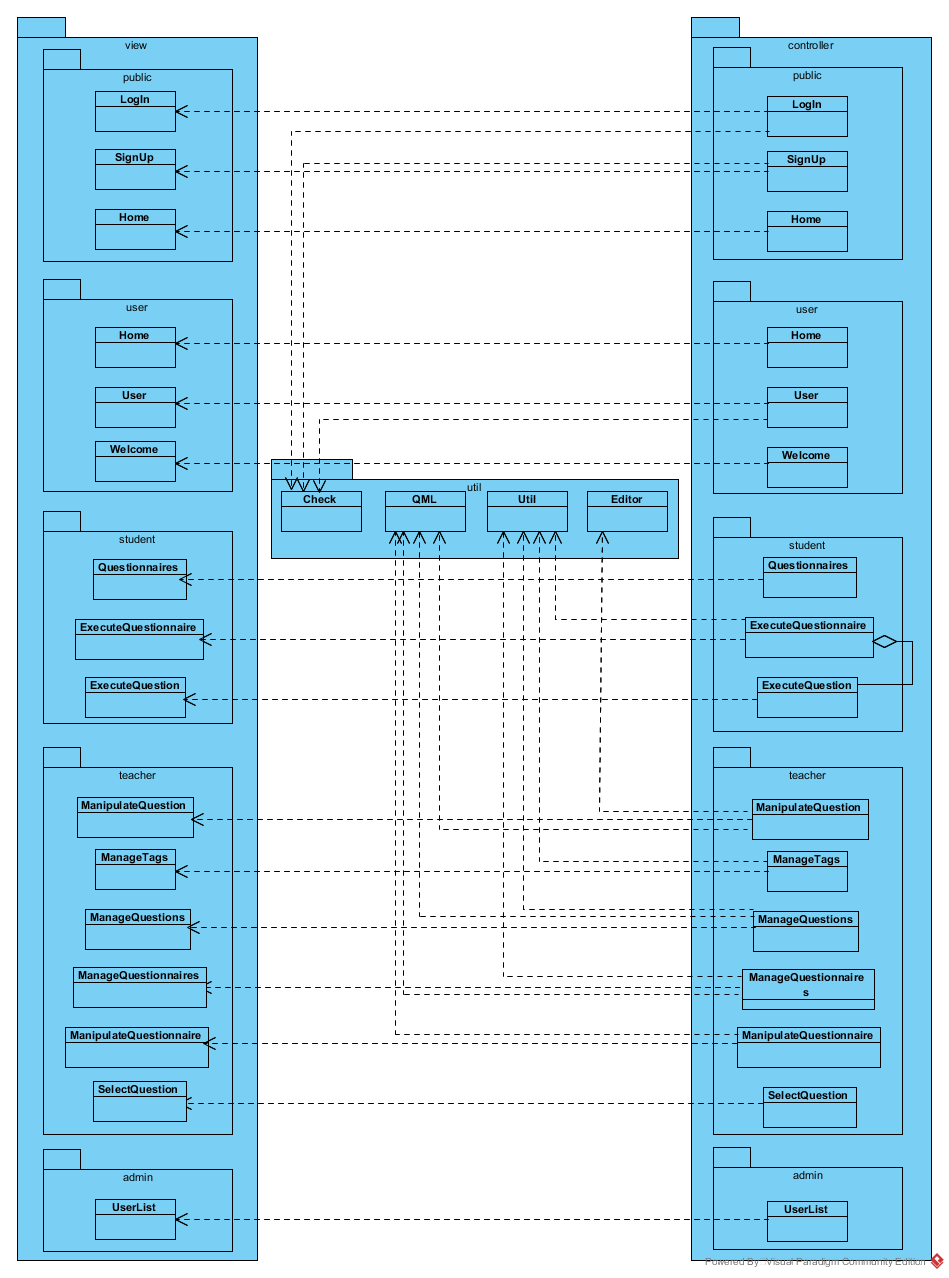
\includegraphics[scale=4, max width=\textwidth, max height=\myheight]{../img/diagrammiClassi/client/viewControllerUtil.png}
		\caption{Diagramma package - client::view, client::controller, client::util}
	\end{figure}
\end{center}

Seguendo si può vedere il diagramma delle classi di \texttt{controller}, \texttt{model} e \texttt{app}.
\begin{center}
	\begin{figure}[H]
		\centering 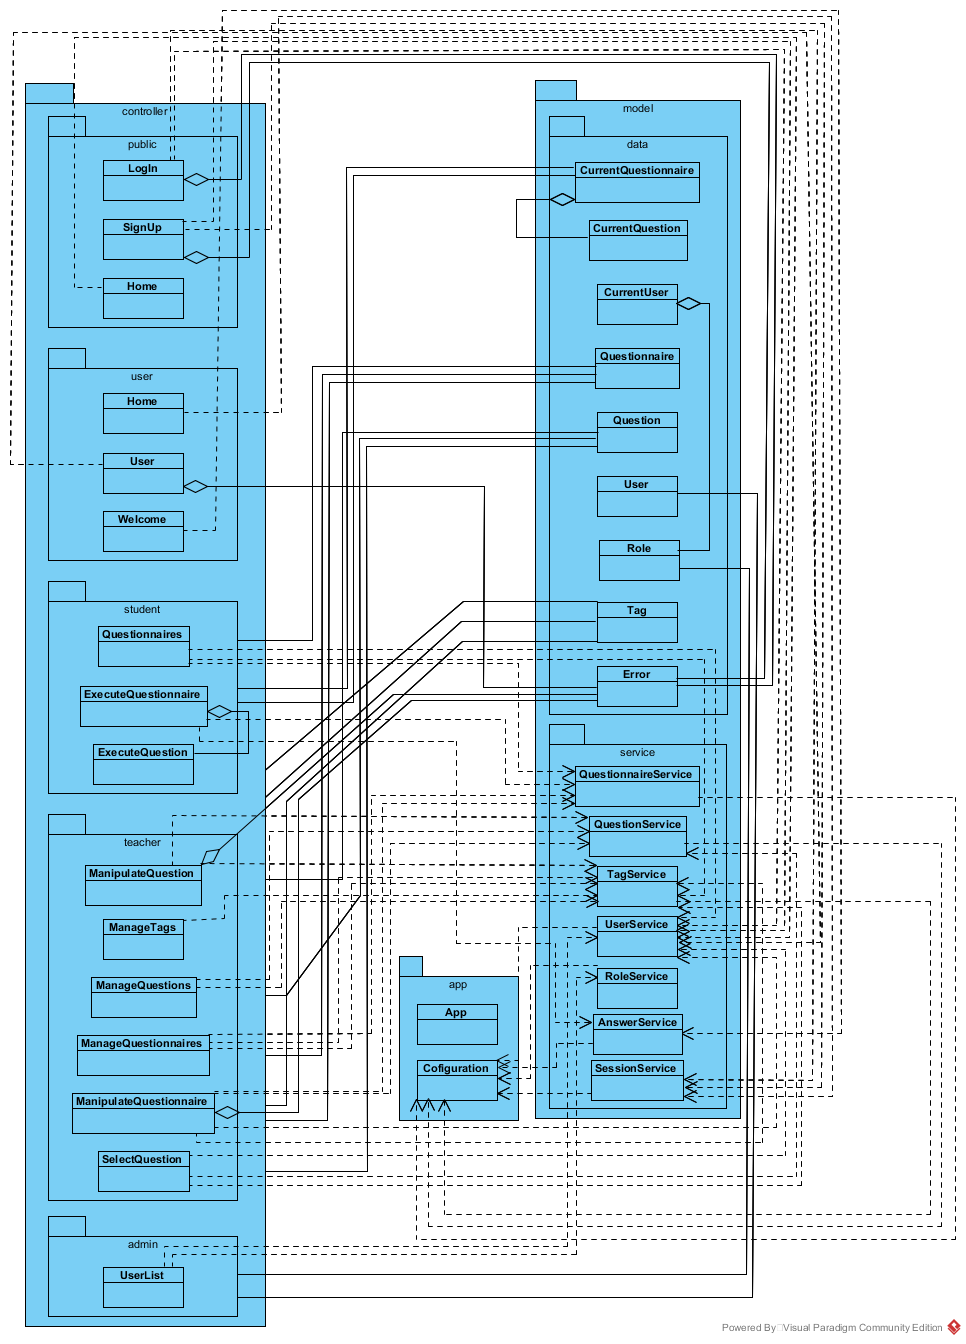
\includegraphics[scale=4, max width=\textwidth, max height=\myheight]{../img/diagrammiClassi/client/controllerModelApp.png}
		\caption{Diagramma package - client::controller, client::model, client::app}
	\end{figure}
\end{center}

\subsection{client::view}
È il package che contiene tutte le classi che costituiscono la view del client. 
Ogni componente si occupa della visualizzazione di una particolare porzione dell'interfaccia di un utente.\begin{center}
	\begin{figure}[H]
		\centering 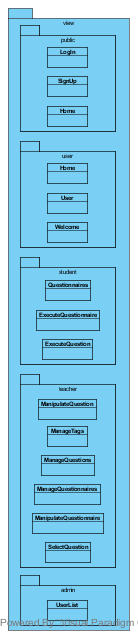
\includegraphics[scale=4, max width=\textwidth, max height=\myheight]{../img/diagrammiClassi/client/view.png}
		\caption{Diagramma package - client::view}
	\end{figure}
\end{center}\subsubsection{client::view::public}
È il package che contiene tutte le classi che costituiscono la view della porzione publica di client. Ogni componente si occupa della visualizzazione di una particolare porzione dell'interfaccia di un utente non autenticato.\begin{center}
	\begin{figure}[H]
		\centering 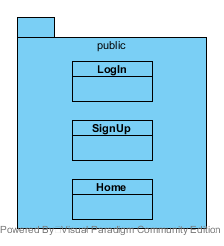
\includegraphics[scale=4, max width=\textwidth, max height=\myheight]{../img/diagrammiClassi/client/view/public.png}
		\caption{Diagramma package - client::view::public}
	\end{figure}
\end{center}\hypertarget{client::view::public::LogIn}{}
\subsubsubsection[LogIn]{client::view::public::LogIn}
\begin{figure}[H]
	\centering
	\begin{tikzpicture}
	\umlclass{client::view::public::LogIn} {}{}
	\end{tikzpicture}
	\caption{Diagramma classe - client::view::public::LogIn}
\end{figure}\begin{description}
\item[Descrizione] \hfill \\
La classe che si occupa della visualizzazione dell'area di autenticazione
\end{description}

\vspace{0.5cm}
\hypertarget{client::view::public::SignUp}{}
\subsubsubsection[SignUp]{client::view::public::SignUp}
\begin{figure}[H]
	\centering
	\begin{tikzpicture}
	\umlclass{client::view::public::SignUp} {}{}
	\end{tikzpicture}
	\caption{Diagramma classe - client::view::public::SignUp}
\end{figure}\begin{description}
\item[Descrizione] \hfill \\
La classe che si occupa della visualizzazione sul client dell'area di registrazione
\end{description}

\vspace{0.5cm}
\hypertarget{client::view::public::Home}{}
\subsubsubsection[Home]{client::view::public::Home}
\begin{figure}[H]
	\centering
	\begin{tikzpicture}
	\umlclass{client::view::public::Home} {}{}
	\end{tikzpicture}
	\caption{Diagramma classe - client::view::public::Home}
\end{figure}\begin{description}
\item[Descrizione] \hfill \\
Classe che si occupa della visualizzazione della home page di un'utente generico
\end{description}

\vspace{0.5cm}
\subsubsection{client::view::student}
È il package che contiene tutte le classi che costituiscono la view della porzione di client per uno studente. Ogni componente si occupa della visualizzazione di una particolare porzione dell'interfaccia di uno studente.\begin{center}
	\begin{figure}[H]
		\centering 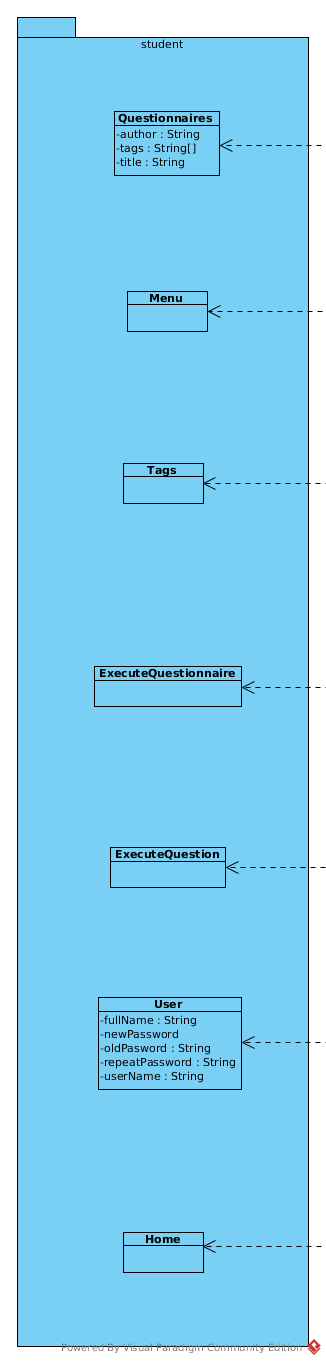
\includegraphics[scale=4, max width=\textwidth, max height=\myheight]{../img/diagrammiClassi/client/view/student.png}
		\caption{Diagramma package - client::view::student}
	\end{figure}
\end{center}\hypertarget{client::view::student::Questionnaires}{}
\subsubsubsection[Questionnaires]{client::view::student::Questionnaires}
\begin{figure}[H]
	\centering
	\begin{tikzpicture}
	\umlclass{client::view::student::Questionnaires} {}{}
	\end{tikzpicture}
	\caption{Diagramma classe - client::view::student::Questionnaires}
\end{figure}\begin{description}
\item[Descrizione] \hfill \\
La classe che si occupa della visualizzazione della lista dei questionari eseguibili
\end{description}

\vspace{0.5cm}
\hypertarget{client::view::student::ExecuteQuestionnaire}{}
\subsubsubsection[ExecuteQuestionnaire]{client::view::student::ExecuteQuestionnaire}
\begin{figure}[H]
	\centering
	\begin{tikzpicture}
	\umlclass{client::view::student::ExecuteQuestionnaire} {}{}
	\end{tikzpicture}
	\caption{Diagramma classe - client::view::student::ExecuteQuestionnaire}
\end{figure}\begin{description}
\item[Descrizione] \hfill \\
La classe che si occupa della visualizzazione di un questionario in esecuzione
\end{description}

\vspace{0.5cm}
\hypertarget{client::view::student::ExecuteQuestion}{}
\subsubsubsection[ExecuteQuestion]{client::view::student::ExecuteQuestion}
\begin{figure}[H]
	\centering
	\begin{tikzpicture}
	\umlclass{client::view::student::ExecuteQuestion} {}{}
	\end{tikzpicture}
	\caption{Diagramma classe - client::view::student::ExecuteQuestion}
\end{figure}\begin{description}
\item[Descrizione] \hfill \\
La classe che si occupa della visualizzazione una domanda in esecuzione
\end{description}

\vspace{0.5cm}
\subsubsection{client::view::teacher}
È il package che contiene tutte le classi che costituiscono la view della porzione di client per un docente. Ogni componente si occupa della visualizzazione di una particolare porzione dell'interfaccia di un docente.\begin{center}
	\begin{figure}[H]
		\centering 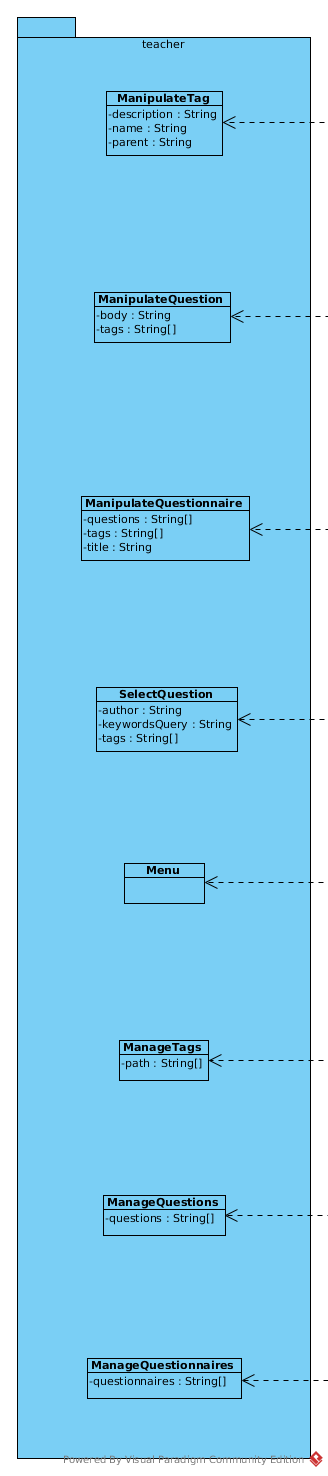
\includegraphics[scale=4, max width=\textwidth, max height=\myheight]{../img/diagrammiClassi/client/view/teacher.png}
		\caption{Diagramma package - client::view::teacher}
	\end{figure}
\end{center}\hypertarget{client::view::teacher::ManipulateQuestion}{}
\subsubsubsection[ManipulateQuestion]{client::view::teacher::ManipulateQuestion}
\begin{figure}[H]
	\centering
	\begin{tikzpicture}
	\umlclass{client::view::teacher::ManipulateQuestion} {}{}
	\end{tikzpicture}
	\caption{Diagramma classe - client::view::teacher::ManipulateQuestion}
\end{figure}\begin{description}
\item[Descrizione] \hfill \\
La classe view che si occupa delle visualizzazione della gestione della domanda
\end{description}

\vspace{0.5cm}
\hypertarget{client::view::teacher::ManipulateQuestionnaire}{}
\subsubsubsection[ManipulateQuestionnaire]{client::view::teacher::ManipulateQuestionnaire}
\begin{figure}[H]
	\centering
	\begin{tikzpicture}
	\umlclass{client::view::teacher::ManipulateQuestionnaire} {}{}
	\end{tikzpicture}
	\caption{Diagramma classe - client::view::teacher::ManipulateQuestionnaire}
\end{figure}\begin{description}
\item[Descrizione] \hfill \\
La classe view che si occupa della visualizzazione della gestione del questionario 
\end{description}

\vspace{0.5cm}
\hypertarget{client::view::teacher::SelectQuestion}{}
\subsubsubsection[SelectQuestion]{client::view::teacher::SelectQuestion}
\begin{figure}[H]
	\centering
	\begin{tikzpicture}
	\umlclass{client::view::teacher::SelectQuestion} {}{}
	\end{tikzpicture}
	\caption{Diagramma classe - client::view::teacher::SelectQuestion}
\end{figure}\begin{description}
\item[Descrizione] \hfill \\
La classe view che si occupa della visualizzazione di selezione delle domande
\end{description}

\vspace{0.5cm}
\hypertarget{client::view::teacher::ManageTags}{}
\subsubsubsection[ManageTags]{client::view::teacher::ManageTags}
\begin{figure}[H]
	\centering
	\begin{tikzpicture}
	\umlclass{client::view::teacher::ManageTags} {}{}
	\end{tikzpicture}
	\caption{Diagramma classe - client::view::teacher::ManageTags}
\end{figure}\begin{description}
\item[Descrizione] \hfill \\
La classe view che si occupa della visualizzazione dell'albero degli argomenti per selezionare un eventuale argomento da gestire
\end{description}

\vspace{0.5cm}
\hypertarget{client::view::teacher::ManageQuestions}{}
\subsubsubsection[ManageQuestions]{client::view::teacher::ManageQuestions}
\begin{figure}[H]
	\centering
	\begin{tikzpicture}
	\umlclass{client::view::teacher::ManageQuestions} {}{}
	\end{tikzpicture}
	\caption{Diagramma classe - client::view::teacher::ManageQuestions}
\end{figure}\begin{description}
\item[Descrizione] \hfill \\
La classe view che si occupa della visualizzazione della lista delle proprie domande per selezionare la domanda da gestire
\end{description}

\vspace{0.5cm}
\hypertarget{client::view::teacher::ManageQuestionnaires}{}
\subsubsubsection[ManageQuestionnaires]{client::view::teacher::ManageQuestionnaires}
\begin{figure}[H]
	\centering
	\begin{tikzpicture}
	\umlclass{client::view::teacher::ManageQuestionnaires} {}{}
	\end{tikzpicture}
	\caption{Diagramma classe - client::view::teacher::ManageQuestionnaires}
\end{figure}\begin{description}
\item[Descrizione] \hfill \\
La classe view che si occupa della visualizzazione della lista dei propri questionari per selezionare il questionario da gestire
\end{description}

\vspace{0.5cm}
\subsubsection{client::view::admin}
È il package che contiene tutte le classi che costituiscono la view della porzione di client per un amministratore. Ogni componente si occupa della visualizzazione di una particolare porzione dell'interfaccia di un amministratore.\begin{center}
	\begin{figure}[H]
		\centering 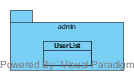
\includegraphics[scale=4, max width=\textwidth, max height=\myheight]{../img/diagrammiClassi/client/view/admin.png}
		\caption{Diagramma package - client::view::admin}
	\end{figure}
\end{center}\hypertarget{client::view::admin::UsersList}{}
\subsubsubsection[UsersList]{client::view::admin::UsersList}
\begin{figure}[H]
	\centering
	\begin{tikzpicture}
	\umlclass{client::view::admin::UsersList} {}{}
	\end{tikzpicture}
	\caption{Diagramma classe - client::view::admin::UsersList}
\end{figure}\begin{description}
\item[Descrizione] \hfill \\
La classe che si occupa della visualizzazione della lista degli utenti.Consente di applicare un filtro ai risultari tra FullName, Role, UserName per la selezione di un utente per la gestione delle sue informazioni.
\end{description}

\vspace{0.5cm}
\subsubsection{client::view::user}
È il package che contiene tutte le classi che costituiscono la view della porzione di client per un'utente generico registrato. Ogni componente si occupa della visualizzazione di una particolare porzione dell'interfaccia di un'utente generico registrato.\begin{center}
	\begin{figure}[H]
		\centering 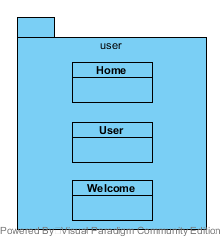
\includegraphics[scale=4, max width=\textwidth, max height=\myheight]{../img/diagrammiClassi/client/view/user.png}
		\caption{Diagramma package - client::view::user}
	\end{figure}
\end{center}\hypertarget{client::view::user::Welcome}{}
\subsubsubsection[Welcome]{client::view::user::Welcome}
\begin{figure}[H]
	\centering
	\begin{tikzpicture}
	\umlclass{client::view::user::Welcome} {}{}
	\end{tikzpicture}
	\caption{Diagramma classe - client::view::user::Welcome}
\end{figure}\begin{description}
\item[Descrizione] \hfill \\
Classe che si occupa della visualizzazione della pagina di benvenuto
\end{description}

\vspace{0.5cm}
\hypertarget{client::view::user::Home}{}
\subsubsubsection[Home]{client::view::user::Home}
\begin{figure}[H]
	\centering
	\begin{tikzpicture}
	\umlclass{client::view::user::Home} {}{}
	\end{tikzpicture}
	\caption{Diagramma classe - client::view::user::Home}
\end{figure}\begin{description}
\item[Descrizione] \hfill \\
Classe che si occupa della visualizzazione della home page di un'utente generico autenticato
\end{description}

\vspace{0.5cm}
\hypertarget{client::view::user::User}{}
\subsubsubsection[User]{client::view::user::User}
\begin{figure}[H]
	\centering
	\begin{tikzpicture}
	\umlclass{client::view::user::User} {}{}
	\end{tikzpicture}
	\caption{Diagramma classe - client::view::user::User}
\end{figure}\begin{description}
\item[Descrizione] \hfill \\
Classe visualizzare la pagina per la gestione del profilo di un'utente generico registrato
\end{description}

\vspace{0.5cm}
\subsection{client::model}
E' il package che contiene le classi dei modelli di dati utilizzati
dal client e i servizi che mettono in comunicazione esso con il server
attraverso i diversi servizi REST.\begin{center}
	\begin{figure}[H]
		\centering 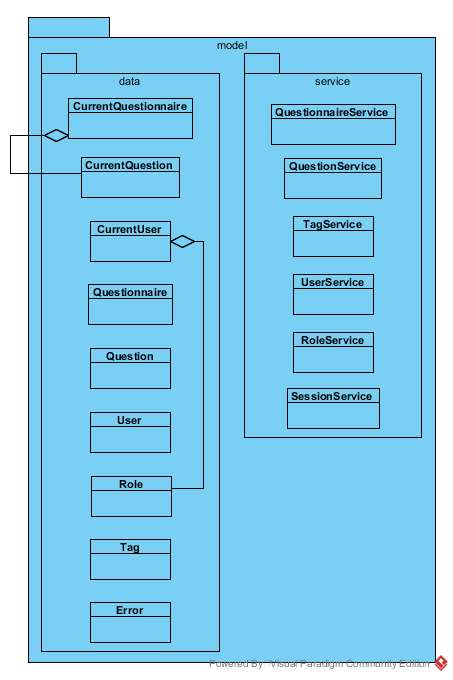
\includegraphics[scale=4, max width=\textwidth, max height=\myheight]{../img/diagrammiClassi/client/model.png}
		\caption{Diagramma package - client::model}
	\end{figure}
\end{center}\subsubsection{client::model::data}
Questo package si occupa della modellazione dei dati utili al client.\begin{center}
	\begin{figure}[H]
		\centering 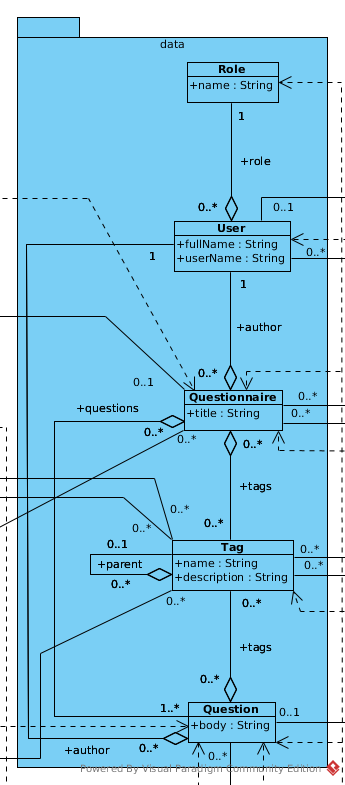
\includegraphics[scale=4, max width=\textwidth, max height=\myheight]{../img/diagrammiClassi/client/model/data.png}
		\caption{Diagramma package - client::model::data}
	\end{figure}
\end{center}\hypertarget{client::model::data::Questionnaire}{}
\subsubsubsection[Questionnaire]{client::model::data::Questionnaire}
\begin{figure}[H]
	\centering
	\begin{tikzpicture}
	\umlclass{client::model::data::Questionnaire} {--questions : String[]\\--tags : String[]\\--author : String\\--title : String\\--id : String}{+Questionnaire(author : String, id : String, questions : String[], tags : String[], title : String)\\+getQuestions() : String[]\\+getTags() : String[]\\+getAuthor() : String\\+getTitle() : String\\+getId() : String\\+setQuestions(questions : String[]) : void\\+setTags(tags : String[]) : void\\+setAuthor(author : String) : void\\+setTitle(title : String) : void\\+setId(id : String) : void}
	\end{tikzpicture}
	\caption{Diagramma classe - client::model::data::Questionnaire}
\end{figure}\begin{description}
\item[Descrizione] \hfill \\
Questa classe modella il tipo di dato "questionario" nella rappresentazione locale dei dati lato client
\item[Relazioni con altre classi] \hfill \\
\vspace{-7mm}
\begin{description}
	\item[\hyperlink{client::controller::teacher::ManipulateQuestionnaire}{client::controller::teacher::ManipulateQuestionnaire}] \hfill \\
	Relazione entrante, oggetto che rappresenta un questionario
	\item[\hyperlink{client::controller::student::Questionnaires}{client::controller::student::Questionnaires}] \hfill \\
	Relazione entrante, lista di questionari
	\item[\hyperlink{client::controller::teacher::ManageQuestionnaires}{client::controller::teacher::ManageQuestionnaires}] \hfill \\
	Relazione entrante, questionari visualizzati nella view
\end{description}

\item[Attributi] \hfill \\
\vspace{-7mm}
\begin{itemize}
	\item questions : String[] $\rightarrow$ insieme di ID di riferimenti a Question
	\item tags : String[] $\rightarrow$ lista di ID di riferimenti ad argomenti 
	\item author : String $\rightarrow$ ID dell'autore del questionario
	\item title : String $\rightarrow$ nome del questionario
	\item id : String $\rightarrow$ ID del Questionnaire
\end{itemize}

\item[Metodi] \hfill \\
\vspace{-7mm}
\begin{itemize}
	\item Questionnaire(author : String, id : String, questions : String[], tags : String[], title : String) $\rightarrow$ costruttore della classe\begin{itemize}
		\item author $\rightarrow$ ID dell'autore del questionario
		\item id $\rightarrow$ ID del Questionnaire
		\item questions $\rightarrow$ insieme di ID di riferimenti a Question
		\item tags $\rightarrow$ lista di ID di riferimenti ad argomenti
		\item title $\rightarrow$ nome del questionario
	\end{itemize}
	
	\item getQuestions() : String[] $\rightarrow$ metodo getter
	\item getTags() : String[] $\rightarrow$ metodo getter
	\item getAuthor() : String $\rightarrow$ metodo getter
	\item getTitle() : String $\rightarrow$ metodo getter
	\item getId() : String $\rightarrow$ metodo getter
	\item setQuestions(questions : String[]) : void $\rightarrow$ metodo setter\begin{itemize}
		\item questions $\rightarrow$ insieme di ID di riferimenti a Question
	\end{itemize}
	
	\item setTags(tags : String[]) : void $\rightarrow$ metodo setter\begin{itemize}
		\item tags $\rightarrow$ lista di ID di riferimenti ad argomenti 
	\end{itemize}
	
	\item setAuthor(author : String) : void $\rightarrow$ metodo setter\begin{itemize}
		\item author $\rightarrow$ ID dell'autore del questionario
	\end{itemize}
	
	\item setTitle(title : String) : void $\rightarrow$ metodo setter\begin{itemize}
		\item title $\rightarrow$ nome del questionario
	\end{itemize}
	
	\item setId(id : String) : void $\rightarrow$ metodo setter\begin{itemize}
		\item id $\rightarrow$ ID del Questionnaire
	\end{itemize}
	
\end{itemize}

\end{description}

\vspace{0.5cm}
\hypertarget{client::model::data::Question}{}
\subsubsubsection[Question]{client::model::data::Question}
\begin{figure}[H]
	\centering
	\begin{tikzpicture}
	\umlclass{client::model::data::Question} {--body : String\\--author : String\\--tags  : String[]\\--id : String}{+Question(author : String, body : String, id : String, tags : String[])\\+getBody() : String\\+getAuthor() : String\\+getTags () : String[]\\+getId() : String\\+setBody(body : String) : void\\+setAuthor(author : String) : void\\+setTags (tags  : String[]) : void\\+setId(id : String) : void}
	\end{tikzpicture}
	\caption{Diagramma classe - client::model::data::Question}
\end{figure}\begin{description}
\item[Descrizione] \hfill \\
Questa classe modella il tipo di dato "domanda" nella rappresentazione locale dei dati lato client
\item[Relazioni con altre classi] \hfill \\
\vspace{-7mm}
\begin{description}
	\item[\hyperlink{client::controller::teacher::ManipulateQuestion}{client::controller::teacher::ManipulateQuestion}] \hfill \\
	Relazione entrante, oggetto che rappresenta una singola domanda
	\item[\hyperlink{client::controller::teacher::ManageQuestions}{client::controller::teacher::ManageQuestions}] \hfill \\
	Relazione entrante, domande visualizzate nella view
	\item[\hyperlink{client::controller::teacher::SelectQuestion}{client::controller::teacher::SelectQuestion}] \hfill \\
	Relazione entrante, domande visualizzate nella view
\end{description}

\item[Attributi] \hfill \\
\vspace{-7mm}
\begin{itemize}
	\item body : String $\rightarrow$ e' la rappresentazione testuale della domanda
	\item author : String $\rightarrow$ ID dell'autore della domanda
	\item tags  : String[] $\rightarrow$ lista di ID di riferimenti ad argomenti
	\item id : String $\rightarrow$ ID della Question
\end{itemize}

\item[Metodi] \hfill \\
\vspace{-7mm}
\begin{itemize}
	\item Question(author : String, body : String, id : String, tags : String[]) $\rightarrow$ costruttore della classe\begin{itemize}
		\item author $\rightarrow$ ID dell'autore della domanda
		\item body $\rightarrow$ e' la rappresentazione testuale della domanda
		\item id $\rightarrow$ ID della Question
		\item tags $\rightarrow$ lista di ID di riferimenti ad argomenti
	\end{itemize}
	
	\item getBody() : String $\rightarrow$ metodo getter
	\item getAuthor() : String $\rightarrow$ metodo getter
	\item getTags () : String[] $\rightarrow$ metodo getter
	\item getId() : String $\rightarrow$ metodo getter
	\item setBody(body : String) : void $\rightarrow$ metodo setter\begin{itemize}
		\item body $\rightarrow$ e' la rappresentazione testuale della domanda
	\end{itemize}
	
	\item setAuthor(author : String) : void $\rightarrow$ metodo setter\begin{itemize}
		\item author $\rightarrow$ ID dell'autore della domanda
	\end{itemize}
	
	\item setTags (tags  : String[]) : void $\rightarrow$ metodo setter\begin{itemize}
		\item tags  $\rightarrow$ lista di ID di riferimenti ad argomenti
	\end{itemize}
	
	\item setId(id : String) : void $\rightarrow$ metodo setter\begin{itemize}
		\item id $\rightarrow$ ID della Question
	\end{itemize}
	
\end{itemize}

\end{description}

\vspace{0.5cm}
\hypertarget{client::model::data::Tag}{}
\subsubsubsection[Tag]{client::model::data::Tag}
\begin{figure}[H]
	\centering
	\begin{tikzpicture}
	\umlclass{client::model::data::Tag} {--name : String\\--description : String\\--id : String}{+Tag(description : String, id : String, name : String)\\+getName() : String\\+getDescription() : String\\+getId() : String\\+setName(name : String) : void\\+setDescription(description : String) : void\\+setId(id : String) : void}
	\end{tikzpicture}
	\caption{Diagramma classe - client::model::data::Tag}
\end{figure}\begin{description}
\item[Descrizione] \hfill \\
Questa classe modella il tag argomento di un questionario e/o di una domanda nella rappresentazione locale dei dati lato client
\item[Relazioni con altre classi] \hfill \\
\vspace{-7mm}
\begin{description}
	\item[\hyperlink{client::controller::teacher::ManageTags}{client::controller::teacher::ManageTags}] \hfill \\
	Relazione entrante, tags visualizzati nella view
	\item[\hyperlink{client::controller::teacher::ManipulateQuestion}{client::controller::teacher::ManipulateQuestion}] \hfill \\
	Relazione entrante, argomenti che compaiono nei suggerimenti
	\item[\hyperlink{client::controller::teacher::ManipulateQuestionnaire}{client::controller::teacher::ManipulateQuestionnaire}] \hfill \\
	Relazione entrante, argomenti che compaiono nei suggerimenti
\end{description}

\item[Attributi] \hfill \\
\vspace{-7mm}
\begin{itemize}
	\item name : String $\rightarrow$ nome dell'argomento
	\item description : String $\rightarrow$ descrizione dell'argomento
	\item id : String $\rightarrow$ ID del Tag
\end{itemize}

\item[Metodi] \hfill \\
\vspace{-7mm}
\begin{itemize}
	\item Tag(description : String, id : String, name : String) $\rightarrow$ costruttore della classe\begin{itemize}
		\item description $\rightarrow$ descrizione dell'argomento
		\item id $\rightarrow$ ID del Tag
		\item name $\rightarrow$ nome dell'argomento
	\end{itemize}
	
	\item getName() : String $\rightarrow$ metodo getter
	\item getDescription() : String $\rightarrow$ metodo getter
	\item getId() : String $\rightarrow$ metodo getter
	\item setName(name : String) : void $\rightarrow$ metodo setter\begin{itemize}
		\item name $\rightarrow$ nome dell'argomento
	\end{itemize}
	
	\item setDescription(description : String) : void $\rightarrow$ metodo setter\begin{itemize}
		\item description $\rightarrow$ descrizione dell'argomento
	\end{itemize}
	
	\item setId(id : String) : void $\rightarrow$ metodo setter\begin{itemize}
		\item id $\rightarrow$ ID del Tag
	\end{itemize}
	
\end{itemize}

\end{description}

\vspace{0.5cm}
\hypertarget{client::model::data::Role}{}
\subsubsubsection[Role]{client::model::data::Role}
\begin{figure}[H]
	\centering
	\begin{tikzpicture}
	\umlclass{client::model::data::Role} {--name : String\\--id : String}{+Role(id : String, name : String)\\+getName() : String\\+getId() : String\\+setName(name : String) : void\\+setId(id : String) : void}
	\end{tikzpicture}
	\caption{Diagramma classe - client::model::data::Role}
\end{figure}\begin{description}
\item[Descrizione] \hfill \\
Questa classe modella il ruolo e i permessi di un utente autenticato nel sistema
\item[Relazioni con altre classi] \hfill \\
\vspace{-7mm}
\begin{description}
	\item[\hyperlink{client::controller::admin::UsersList}{client::controller::admin::UsersList}] \hfill \\
	Relazione entrante, lista di tutti i ruoli che può assumere un utente
	\item[\hyperlink{client::model::data::CurrentUser}{client::model::data::CurrentUser}] \hfill \\
	Relazione entrante, role del ruolo dell'utente
\end{description}

\item[Attributi] \hfill \\
\vspace{-7mm}
\begin{itemize}
	\item name : String $\rightarrow$ e' il ruolo che un utente può assumere
	\item id : String $\rightarrow$ ID del Role
\end{itemize}

\item[Metodi] \hfill \\
\vspace{-7mm}
\begin{itemize}
	\item Role(id : String, name : String) $\rightarrow$ costruttore della classe\begin{itemize}
		\item id $\rightarrow$ ID del Role
		\item name $\rightarrow$ e' il ruolo che un utente può assumere
	\end{itemize}
	
	\item getName() : String $\rightarrow$ metodo getter
	\item getId() : String $\rightarrow$ metodo getter
	\item setName(name : String) : void $\rightarrow$ metodo setter\begin{itemize}
		\item name $\rightarrow$ e' il ruolo che un utente può assumere
	\end{itemize}
	
	\item setId(id : String) : void $\rightarrow$ metodo setter\begin{itemize}
		\item id $\rightarrow$ ID del Role
	\end{itemize}
	
\end{itemize}

\end{description}

\vspace{0.5cm}
\hypertarget{client::model::data::User}{}
\subsubsubsection[User]{client::model::data::User}
\begin{figure}[H]
	\centering
	\begin{tikzpicture}
	\umlclass{client::model::data::User} {--role : String\\--fullName : String\\--userName : String\\--id : String}{+User(fullName : String, id : String, role : String, userName : String)\\+getRole() : String\\+getFullName() : String\\+getUserName() : String\\+getId() : String\\+setRole(role : String) : void\\+setFullName(fullName : String) : void\\+setUserName(userName : String) : void\\+setId(id : String) : void}
	\end{tikzpicture}
	\caption{Diagramma classe - client::model::data::User}
\end{figure}\begin{description}
\item[Descrizione] \hfill \\
Questa classe modella le informazioni del profilo di un utente autenticato nel sistema
\item[Relazioni con altre classi] \hfill \\
\vspace{-7mm}
\begin{description}
	\item[\hyperlink{client::controller::admin::UsersList}{client::controller::admin::UsersList}] \hfill \\
	Relazione entrante, lista di utenti
\end{description}

\item[Attributi] \hfill \\
\vspace{-7mm}
\begin{itemize}
	\item role : String $\rightarrow$ ID del Role del ruolo dell'utente
	\item fullName : String $\rightarrow$ nome completo dell'utente
	\item userName : String $\rightarrow$ userName dell'utente
	\item id : String $\rightarrow$ ID dell'User
\end{itemize}

\item[Metodi] \hfill \\
\vspace{-7mm}
\begin{itemize}
	\item User(fullName : String, id : String, role : String, userName : String) $\rightarrow$ costruttore della classe\begin{itemize}
		\item fullName $\rightarrow$ nome completo dell'utente
		\item id $\rightarrow$ ID dell'User
		\item role $\rightarrow$ ID del Role del ruolo dell'utente
		\item userName $\rightarrow$ userName dell'utente
	\end{itemize}
	
	\item getRole() : String $\rightarrow$ metodo getter
	\item getFullName() : String $\rightarrow$ metodo getter
	\item getUserName() : String $\rightarrow$ metodo getter
	\item getId() : String $\rightarrow$ metodo getter
	\item setRole(role : String) : void $\rightarrow$ metodo setter\begin{itemize}
		\item role $\rightarrow$ ID del Role del ruolo dell'utente
	\end{itemize}
	
	\item setFullName(fullName : String) : void $\rightarrow$ metodo setter\begin{itemize}
		\item fullName $\rightarrow$ nome completo dell'utente
	\end{itemize}
	
	\item setUserName(userName : String) : void $\rightarrow$ metodo setter\begin{itemize}
		\item userName $\rightarrow$ userName dell'utente
	\end{itemize}
	
	\item setId(id : String) : void $\rightarrow$ metodo setter\begin{itemize}
		\item id $\rightarrow$ ID dell'User
	\end{itemize}
	
\end{itemize}

\end{description}

\vspace{0.5cm}
\hypertarget{client::model::data::CurrentQuestion}{}
\subsubsubsection[CurrentQuestion]{client::model::data::CurrentQuestion}
\begin{figure}[H]
	\centering
	\begin{tikzpicture}
	\umlclass{client::model::data::CurrentQuestion} {--body : String\\--answer : String\\--type : String\\--answers : String []\\--selectedAnswer : String}{+CurrentQuestion(question : Question)\\+point() : Json\\+getBody() : String\\+getAnswer() : String\\+getType() : String\\+setBody(body : String) : void\\+setAnswer(answer : String) : void\\+setType(type : String) : void\\+getAnswers() : String []\\+getSelectedAnswer() : String\\+setAnswers(answers : String []) : void\\+setSelectedAnswer(selectedAnswer : String) : void}
	\end{tikzpicture}
	\caption{Diagramma classe - client::model::data::CurrentQuestion}
\end{figure}\begin{description}
\item[Descrizione] \hfill \\
La classe che modella la domanda in esecuzione
\item[Relazioni con altre classi] \hfill \\
\vspace{-7mm}
\begin{description}
	\item[\hyperlink{client::model::data::CurrentQuestionnaire}{client::model::data::CurrentQuestionnaire}] \hfill \\
	Relazione entrante, lista di domande del questionario corrente
\end{description}

\item[Attributi] \hfill \\
\vspace{-7mm}
\begin{itemize}
	\item body : String $\rightarrow$ contiene il corpo della domanda corrente 
	\item answer : String $\rightarrow$ contiene la risposta alla domanda corrente
	\item type : String $\rightarrow$ oggetto che rappresenta la tipologia della domanda
	\item answers : String [] $\rightarrow$ oggetto che rappresenta una lista di risposte
	\item selectedAnswer : String $\rightarrow$ oggetto che rappresenta la risposta selezionata
\end{itemize}

\item[Metodi] \hfill \\
\vspace{-7mm}
\begin{itemize}
	\item CurrentQuestion(question : Question) $\rightarrow$ costruttore della classe\begin{itemize}
		\item question $\rightarrow$ contiene il riferimento all'oggetto Question associato
	\end{itemize}
	
	\item point() : Json $\rightarrow$ restituisce i punti relativi alla domanda risposta
	
	Metodo che restituisce un oggetto di tipo json con attributi 'point' e 'tot' che contengono due interi rappresentanti i punti totalizzati sui punti totali del risposta
	\item getBody() : String $\rightarrow$ metodo getter
	\item getAnswer() : String $\rightarrow$ metodo getter
	\item getType() : String $\rightarrow$ metodo getter
	\item setBody(body : String) : void $\rightarrow$ metodo setter\begin{itemize}
		\item body $\rightarrow$ contiene il corpo della domanda corrente 
	\end{itemize}
	
	\item setAnswer(answer : String) : void $\rightarrow$ metodo setter\begin{itemize}
		\item answer $\rightarrow$ contiene la risposta alla domanda corrente
	\end{itemize}
	
	\item setType(type : String) : void $\rightarrow$ metodo setter\begin{itemize}
		\item type $\rightarrow$ oggetto che rappresenta la tipologia della domanda
	\end{itemize}
	
	\item getAnswers() : String [] $\rightarrow$ metodo getter
	\item getSelectedAnswer() : String $\rightarrow$ metodo getter
	\item setAnswers(answers : String []) : void $\rightarrow$ metodo setter\begin{itemize}
		\item answers $\rightarrow$ oggetto che rappresenta una lista di risposte
	\end{itemize}
	
	\item setSelectedAnswer(selectedAnswer : String) : void $\rightarrow$ metodo setter\begin{itemize}
		\item selectedAnswer $\rightarrow$ oggetto che rappresenta la risposta selezionata
	\end{itemize}
	
\end{itemize}

\end{description}

\vspace{0.5cm}
\hypertarget{client::model::data::CurrentQuestionnaire}{}
\subsubsubsection[CurrentQuestionnaire]{client::model::data::CurrentQuestionnaire}
\begin{figure}[H]
	\centering
	\begin{tikzpicture}
	\umlclass{client::model::data::CurrentQuestionnaire} {--tags : String[]\\--currentNumber : int\\--questionNumber : int\\--questions : CurrentQuestion[]\\--title : String}{+getNext () : CurrentQuestion\\+getPrevious() : CurrentQuestion\\+checkAnswers() : boolean\\+CurrentQuestionnaire(questions : CurrentQuestion[], tags : String[], title : String)\\+getResult() : Json\\+getTags() : String[]\\+getCurrentNumber() : int\\+getQuestionNumber() : int\\+getQuestions() : CurrentQuestion[]\\+getTitle() : String[]\\+setTags(tags : String[]) : void\\+setCurrentNumber(currentNumber : int) : void\\+setQuestionNumber(questionNumber : int) : void\\+setQuestions(questions : CurrentQuestion[]) : void\\+setTitle(title : String[]) : void}
	\end{tikzpicture}
	\caption{Diagramma classe - client::model::data::CurrentQuestionnaire}
\end{figure}\begin{description}
\item[Descrizione] \hfill \\
La classe che modella il questionario in esecuzione
\item[Relazioni con altre classi] \hfill \\
\vspace{-7mm}
\begin{description}
	\item[\hyperlink{client::model::data::CurrentQuestion}{client::model::data::CurrentQuestion}] \hfill \\
	Relazione uscente, lista di domande del questionario corrente
	\item[\hyperlink{client::controller::student::ExecuteQuestionnaire}{client::controller::student::ExecuteQuestionnaire}] \hfill \\
	Relazione entrante, istanza del questionario in esecuzione
\end{description}

\item[Attributi] \hfill \\
\vspace{-7mm}
\begin{itemize}
	\item tags : String[] $\rightarrow$ contiene la lista degli argomenti del questionario
	\item currentNumber : int $\rightarrow$ contiene numero della domanda corrente che si sta eseguendo
	\item questionNumber : int $\rightarrow$ contiene il numero totale delle domande nel questionario corrente
	\item questions : CurrentQuestion[] $\rightarrow$ lista di domande del questionario corrente
	\item title : String $\rightarrow$ titolo del questionario corrente
\end{itemize}

\item[Metodi] \hfill \\
\vspace{-7mm}
\begin{itemize}
	\item getNext () : CurrentQuestion $\rightarrow$ metodo che ritorna la prossima domanda
	\item getPrevious() : CurrentQuestion $\rightarrow$ metodo che ritorna la domanda precedente
	\item checkAnswers() : boolean $\rightarrow$ metodo che controlla che tutte le domande abbiano una risposta data, restituendo vero in caso positivo, falso altrimenti
	\item CurrentQuestionnaire(questions : CurrentQuestion[], tags : String[], title : String) $\rightarrow$ costruttore della classe\begin{itemize}
		\item questions $\rightarrow$ lista di domande del questionario corrente
		\item tags $\rightarrow$ contiene la lista degli argomenti del questionario
		\item title $\rightarrow$ titolo del questionario corrente
	\end{itemize}
	
	\item getResult() : Json $\rightarrow$ metodo che restituisce un oggetto di tipo json con attributi 'point' e 'tot' che contengono due interi rappresentanti i punti totalizzati sui punti totali del questionario
	\item getTags() : String[] $\rightarrow$ metodo getter
	\item getCurrentNumber() : int $\rightarrow$ metodo getter
	\item getQuestionNumber() : int $\rightarrow$ metodo getter
	\item getQuestions() : CurrentQuestion[] $\rightarrow$ metodo getter
	\item getTitle() : String[] $\rightarrow$ metodo getter
	\item setTags(tags : String[]) : void $\rightarrow$ metodo setter\begin{itemize}
		\item tags $\rightarrow$ contiene la lista degli argomenti del questionario
	\end{itemize}
	
	\item setCurrentNumber(currentNumber : int) : void $\rightarrow$ metodo setter\begin{itemize}
		\item currentNumber $\rightarrow$  Contiene numero della domanda corrente che si sta eseguendo
	\end{itemize}
	
	\item setQuestionNumber(questionNumber : int) : void $\rightarrow$ metodo setter\begin{itemize}
		\item questionNumber $\rightarrow$ contiene il numero totale delle domande nel questionario corrente
	\end{itemize}
	
	\item setQuestions(questions : CurrentQuestion[]) : void $\rightarrow$ metodo setter\begin{itemize}
		\item questions $\rightarrow$ lista di domande del questionario corrente
	\end{itemize}
	
	\item setTitle(title : String[]) : void $\rightarrow$ metodo setter\begin{itemize}
		\item title $\rightarrow$ titolo del questionario corrente
	\end{itemize}
	
\end{itemize}

\end{description}

\vspace{0.5cm}
\hypertarget{client::model::data::CurrentUser}{}
\subsubsubsection[CurrentUser]{client::model::data::CurrentUser}
\begin{figure}[H]
	\centering
	\begin{tikzpicture}
	\umlclass{client::model::data::CurrentUser} {--fullName : String\\--id : String\\--role : Role\\--userName : String}{+CurrentUser(fullName : String, id : String, role : Role, userName : String)\\+getFullName() : String\\+getId() : String\\+getRole() : Role\\+getUserName() : String\\+setFullName(fullName : String) : void\\+setId(id : String) : void\\+setRole(role : Role) : void\\+setUserName(userName : String) : void}
	\end{tikzpicture}
	\caption{Diagramma classe - client::model::data::CurrentUser}
\end{figure}\begin{description}
\item[Descrizione] \hfill \\
La classe che modella un l'utente correntemente loggato

\item[Relazioni con altre classi] \hfill \\
\vspace{-7mm}
\begin{description}
	\item[\hyperlink{client::model::data::Role}{client::model::data::Role}] \hfill \\
	Relazione uscente, role del ruolo dell'utente
\end{description}

\item[Attributi] \hfill \\
\vspace{-7mm}
\begin{itemize}
	\item fullName : String $\rightarrow$ nome completo dell'utente
	\item id : String $\rightarrow$ ID dell'User
	\item role : Role $\rightarrow$ Role del ruolo dell'utente
	\item userName : String $\rightarrow$ userName dell'utente
\end{itemize}

\item[Metodi] \hfill \\
\vspace{-7mm}
\begin{itemize}
	\item CurrentUser(fullName : String, id : String, role : Role, userName : String) $\rightarrow$ costruttore della classe\begin{itemize}
		\item fullName $\rightarrow$ nome completo dell'utente
		\item id $\rightarrow$ ID dell'User
		\item role $\rightarrow$ Role del ruolo dell'utente
		\item userName $\rightarrow$ userName dell'utente
	\end{itemize}
	
	\item getFullName() : String $\rightarrow$ metodo getter
	\item getId() : String $\rightarrow$ metodo getter
	\item getRole() : Role $\rightarrow$ metodo getter
	\item getUserName() : String $\rightarrow$ metodo getter
	\item setFullName(fullName : String) : void $\rightarrow$ metodo setter\begin{itemize}
		\item fullName $\rightarrow$ nome completo dell'utente	
	\end{itemize}
	
	\item setId(id : String) : void $\rightarrow$ metodo setter\begin{itemize}
		\item id $\rightarrow$ ID dell'User
	\end{itemize}
	
	\item setRole(role : Role) : void $\rightarrow$ metodo setter\begin{itemize}
		\item role $\rightarrow$ role del ruolo dell'utente
	\end{itemize}
	
	\item setUserName(userName : String) : void $\rightarrow$ metodo setter\begin{itemize}
		\item userName $\rightarrow$ userName dell'utente
	\end{itemize}
	
\end{itemize}

\end{description}

\vspace{0.5cm}
\hypertarget{client::model::data::Error}{}
\subsubsubsection[Error]{client::model::data::Error}
\begin{figure}[H]
	\centering
	\begin{tikzpicture}
	\umlclass{client::model::data::Error} {--message : String\\--name : String\\--type : String\\--status : boolean}{+Error(status : boolean, message : String, type : String, name : String)\\+getMessage() : String\\+getName() : String\\+getType() : String\\+getStatus() : boolean\\+setMessage(message : String) : void\\+setName(name : String) : void\\+setType(type : String) : void\\+setStatus(status : boolean) : void}
	\end{tikzpicture}
	\caption{Diagramma classe - client::model::data::Error}
\end{figure}\begin{description}
\item[Descrizione] \hfill \\
Classe che rappresenta un errore da visualizzare all'utente
\item[Relazioni con altre classi] \hfill \\
\vspace{-7mm}
\begin{description}
	\item[\hyperlink{client::controller::public::LogIn}{client::controller::public::LogIn}] \hfill \\
	Relazione entrante, campo dati che rappresenta un oggetto Error
	\item[\hyperlink{client::controller::public::SignUp}{client::controller::public::SignUp}] \hfill \\
	Relazione entrante, oggetto che rappresenta un errore da visualizzare all'utente
	\item[\hyperlink{client::controller::user::User}{client::controller::user::User}] \hfill \\
	Relazione entrante, oggetto che rappresenta un errore da visualizzare all'utente sulla password
	\item[\hyperlink{client::controller::user::User}{client::controller::user::User}] \hfill \\
	Relazione entrante, oggetto che rappresenta un errore da visualizzare all'utente sui dati inseriti
	\item[\hyperlink{client::controller::teacher::ManipulateQuestion}{client::controller::teacher::ManipulateQuestion}] \hfill \\
	Relazione entrante, campo dati che rappresenta un oggetto Error
	\item[\hyperlink{client::controller::teacher::ManipulateQuestionnaire}{client::controller::teacher::ManipulateQuestionnaire}] \hfill \\
	Relazione entrante, campo dati che rappresenta un oggetto Error
\end{description}

\item[Attributi] \hfill \\
\vspace{-7mm}
\begin{itemize}
	\item message : String $\rightarrow$ rappresenta il messaggio da visualizzare
	\item name : String $\rightarrow$ nome dell'errore
	\item type : String $\rightarrow$ tipologia dell'errore
	\item status : boolean $\rightarrow$ rappresenta se l'errore è nascosto o no nella vista
\end{itemize}

\item[Metodi] \hfill \\
\vspace{-7mm}
\begin{itemize}
	\item Error(status : boolean, message : String, type : String, name : String) $\rightarrow$ costruttore della classe\begin{itemize}
		\item status $\rightarrow$ rappresenta se l'errore è nascosto o no nella vista
		\item message $\rightarrow$ rappresenta il messaggio da visualizzare
		\item type $\rightarrow$ tipologia dell'errore
		\item name $\rightarrow$ nome dell'errore
	\end{itemize}
	
	\item getMessage() : String $\rightarrow$ metodo getter
	\item getName() : String $\rightarrow$ metodo getter
	\item getType() : String $\rightarrow$ metodo getter
	\item getStatus() : boolean $\rightarrow$ metodo getter
	\item setMessage(message : String) : void $\rightarrow$ metodo setter\begin{itemize}
		\item message $\rightarrow$ rappresenta il messaggio da visualizzare
	\end{itemize}
	
	\item setName(name : String) : void $\rightarrow$ metodo setter\begin{itemize}
		\item name $\rightarrow$ nome dell'errore
	\end{itemize}
	
	\item setType(type : String) : void $\rightarrow$ metodo setter\begin{itemize}
		\item type $\rightarrow$ tipologia dell'errore
	\end{itemize}
	
	\item setStatus(status : boolean) : void $\rightarrow$ metodo setter\begin{itemize}
		\item status $\rightarrow$ rappresenta se l'errore è nascosto o no nella vista
	\end{itemize}
	
\end{itemize}

\end{description}

\vspace{0.5cm}
\subsubsection{client::model::service}
Questo package contiene le classi che gestiscono il recupero dei dati, che siano essi salvati in locale o recuperabili dall'interfaccia server tramite le Api REST.\begin{center}
	\begin{figure}[H]
		\centering 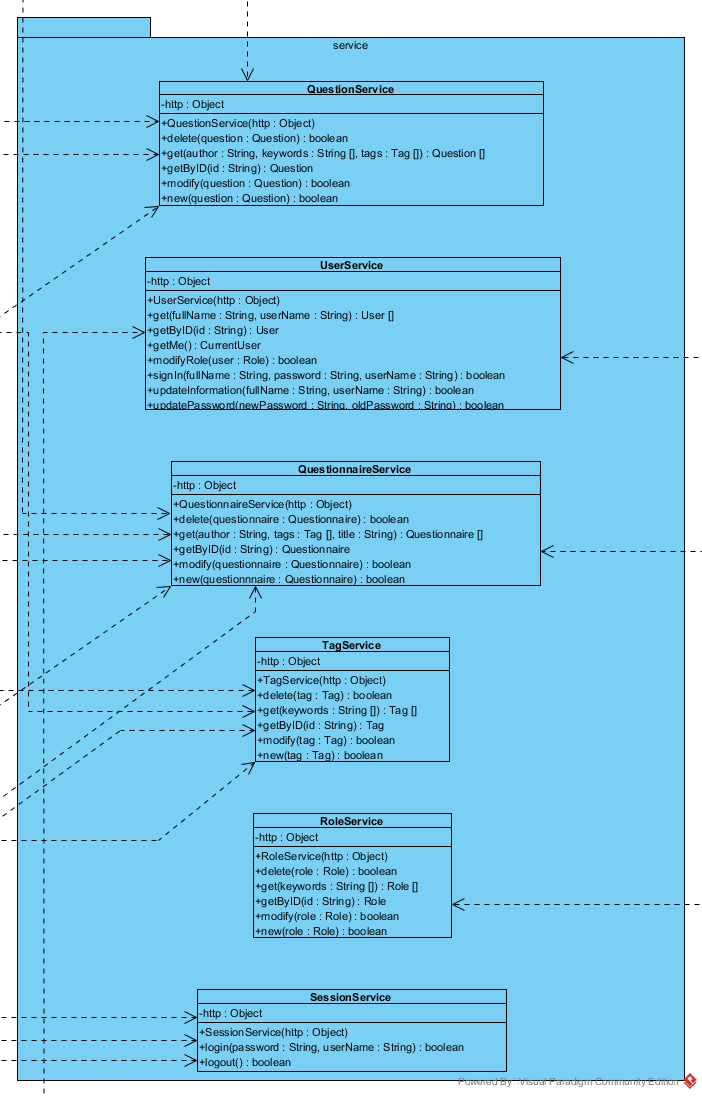
\includegraphics[scale=4, max width=\textwidth, max height=\myheight]{../img/diagrammiClassi/client/model/service.png}
		\caption{Diagramma package - client::model::service}
	\end{figure}
\end{center}\hypertarget{client::model::service::SessionService}{}
\subsubsubsection[SessionService]{client::model::service::SessionService}
\begin{figure}[H]
	\centering
	\begin{tikzpicture}
	\umlclass{client::model::service::SessionService} {--http : Object\\--configuration : Configuration}{+SessionService(http : Object, configuration : Configuration)\\+login(password : String, userName : String, next : Function, err : Function) : void\\+logout(next : Function, err : Function) : void}
	\end{tikzpicture}
	\caption{Diagramma classe - client::model::service::SessionService}
\end{figure}\begin{description}
\item[Descrizione] \hfill \\
Questa classe fornisce al client i servizi relativi  alle credenziali accesso di un utente
\item[Relazioni con altre classi] \hfill \\
\vspace{-7mm}
\begin{description}
	\item[\hyperlink{client::controller::public::LogIn}{client::controller::public::LogIn}] \hfill \\
	Relazione entrante, campo dati che rappresenta un oggetto SessionService
	\item[\hyperlink{client::controller::user::Home}{client::controller::user::Home}] \hfill \\
	Relazione entrante, campo dati che rappresenta un oggetto SessionService
	\item[\hyperlink{client::app::Configuration}{client::app::Configuration}] \hfill \\
	Relazione uscente, campo dati che rappresenta un oggetto Configuration
	\item[\hyperlink{client::controller::public::SignUp}{client::controller::public::SignUp}] \hfill \\
	Relazione entrante, campo dati che rappresenta un oggetto SessionService
\end{description}

\item[Attributi] \hfill \\
\vspace{-7mm}
\begin{itemize}
	\item http : Object $\rightarrow$ oggetto del servizio offerto da angulajs per le richieste http
	\item configuration : Configuration $\rightarrow$ campo dati che rappresenta un oggetto Configuration
\end{itemize}

\item[Metodi] \hfill \\
\vspace{-7mm}
\begin{itemize}
	\item SessionService(http : Object, configuration : Configuration) $\rightarrow$ costruttore della classe\begin{itemize}
		\item http $\rightarrow$ oggetto del servizio offerto da angulajs per le richieste http
		\item configuration $\rightarrow$ campo dati che rappresenta un oggetto Configuration
	\end{itemize}
	
	\item login(password : String, userName : String, next : Function, err : Function) : void $\rightarrow$ provedde ad effettuare l'accesso presso il server\begin{itemize}
		\item password $\rightarrow$ contiene la password inserita dall'utente
		\item userName $\rightarrow$ contiene l'username inserito dall'utente
		\item next $\rightarrow$ questo parametro rappresenta la callback che il metodo chimama in caso di successo
		\item err $\rightarrow$ questo parametro rappresenta la callback che il metodo chimama in caso di errore
	\end{itemize}
	
	\item logout(next : Function, err : Function) : void $\rightarrow$ chiude la sessione dell'utente\begin{itemize}
		\item next $\rightarrow$ questo parametro rappresenta la callback che il metodo chimama in caso di successo
		\item err $\rightarrow$ questo parametro rappresenta la callback che il metodo chimama in caso di errore
	\end{itemize}
	
\end{itemize}

\end{description}

\vspace{0.5cm}
\hypertarget{client::model::service::UserService}{}
\subsubsubsection[UserService]{client::model::service::UserService}
\begin{figure}[H]
	\centering
	\leftskip-1cm
	\begin{tikzpicture}
	\umlclass{client::model::service::UserService} {--http : Object\\--configuration : Configuration\\--roleService : RoleService}{+UserService(http : Object)\\+get(fullName : String[], userName : String[], next : Function, err : Function) : void\\+getByID(id : String, next : Function, err : Function) : void\\+getMe(next : Function, err : Function) : void\\+signUp(fullName : String, password : String, userName : String, next : Function, err : Function) : void\\+updateInformation(fullName : String, userName : String, next : Function, err : Function) : void\\+updatePassword(newPassword : String, oldPassword : String, next : Function, err : Function) : void\\+modifyRole(user : User, role : Role, next : Function, err : Function) : void\\+delete(user : User, next : Function, err : Function) : void}
	\end{tikzpicture}
	\caption{Diagramma classe - client::model::service::UserService}
\end{figure}\begin{description}
\item[Descrizione] \hfill \\
Questa classe fornisce al client i servizi relativi al profilo 
\item[Relazioni con altre classi] \hfill \\
\vspace{-7mm}
\begin{description}
	\item[\hyperlink{client::controller::public::LogIn}{client::controller::public::LogIn}] \hfill \\
	Relazione entrante, campo dati che rappresenta un oggetto UserService
	\item[\hyperlink{client::controller::user::User}{client::controller::user::User}] \hfill \\
	Relazione entrante, campo dati che rappresenta un oggetto UserService
	\item[\hyperlink{client::app::Configuration}{client::app::Configuration}] \hfill \\
	Relazione uscente, campo dati che rappresenta un oggetto Configuration
	\item[\hyperlink{client::model::service::RoleService}{client::model::service::RoleService}] \hfill \\
	Relazione uscente, campo dati che rappresenta un oggetto RoleService
	\item[\hyperlink{client::controller::student::Questionnaires}{client::controller::student::Questionnaires}] \hfill \\
	Relazione entrante, campo dati che rappresenta un oggetto UserService
	\item[\hyperlink{client::controller::teacher::ManipulateQuestionnaire}{client::controller::teacher::ManipulateQuestionnaire}] \hfill \\
	Relazione entrante, campo dati che rappresenta un oggetto UserService
	\item[\hyperlink{client::controller::teacher::SelectQuestion}{client::controller::teacher::SelectQuestion}] \hfill \\
	Relazione entrante, campo dati che rappresenta un oggetto UserService
	\item[\hyperlink{client::controller::public::SignUp}{client::controller::public::SignUp}] \hfill \\
	Relazione entrante, campo dati che rappresenta un oggetto UserService
	\item[\hyperlink{client::controller::public::Home}{client::controller::public::Home}] \hfill \\
	Relazione entrante, campo dati che rappresenta un oggetto UserService
	\item[\hyperlink{client::controller::admin::UsersList}{client::controller::admin::UsersList}] \hfill \\
	Relazione entrante, campo dati che rappresenta un oggetto UserService
\end{description}

\item[Attributi] \hfill \\
\vspace{-7mm}
\begin{itemize}
	\item http : Object $\rightarrow$ oggetto del servizio offerto da angulajs per le richieste http
	\item configuration : Configuration $\rightarrow$ campo dati che rappresenta un oggetto Configuration
	\item roleService : RoleService $\rightarrow$ campo dati che rappresenta un oggetto RoleService
\end{itemize}

\item[Metodi] \hfill \\
\vspace{-7mm}
\begin{itemize}
	\item UserService(http : Object) $\rightarrow$ costruttore della classe\begin{itemize}
		\item http $\rightarrow$ oggetto del servizio offerto da angulajs per le richieste http
	\end{itemize}
	
	\item get(fullName : String[], userName : String[], next : Function, err : Function) : void $\rightarrow$ tramite API REST ritorna una lista di utenti sul server filtrate in base ai parametri\begin{itemize}
		\item fullName $\rightarrow$ contiene il nome del utente da ricercare 
		\item userName $\rightarrow$ contiene il username dell'utente da ricercare 
		\item next $\rightarrow$ questo parametro rappresenta la callback che il metodo chimama in caso di successo
		\item err $\rightarrow$ questo parametro rappresenta la callback che il metodo chimama in caso di errore
	\end{itemize}
	
	\item getByID(id : String, next : Function, err : Function) : void $\rightarrow$ tramite API REST ritorna un utente dal server per ID\begin{itemize}
		\item id $\rightarrow$ contiene id dell'utente da ricercare 
		\item next $\rightarrow$ questo parametro rappresenta la callback che il metodo chimama in caso di successo
		\item err $\rightarrow$ questo parametro rappresenta la callback che il metodo chimama in caso di errore
	\end{itemize}
	
	\item getMe(next : Function, err : Function) : void $\rightarrow$ tramite API REST ritorna l'utente corrente\begin{itemize}
		\item next $\rightarrow$ questo parametro rappresenta la callback che il metodo chimama in caso di successo
		\item err $\rightarrow$ questo parametro rappresenta la callback che il metodo chimama in caso di errore
	\end{itemize}
	
	\item signUp(fullName : String, password : String, userName : String, next : Function, err : Function) : void $\rightarrow$ tramite API REST crea un nuovo utente sul server\begin{itemize}
		\item fullName $\rightarrow$ contiene il nome del nuovo utente
		\item password $\rightarrow$ contiene la password del nuovo utente
		\item userName $\rightarrow$ contiene il username del nuovo utente
		\item next $\rightarrow$ questo parametro rappresenta la callback che il metodo chimama in caso di successo
		\item err $\rightarrow$ questo parametro rappresenta la callback che il metodo chimama in caso di errore
	\end{itemize}
	
	\item updateInformation(fullName : String, userName : String, next : Function, err : Function) : void $\rightarrow$ tramite API REST modifica le informazioni di profilo dell'utente corrente sul server\begin{itemize}
		\item fullName $\rightarrow$ contiene il nuovo nome dell'utente
		\item userName $\rightarrow$ contiene il nuovo username dell'utente
		\item next $\rightarrow$ questo parametro rappresenta la callback che il metodo chimama in caso di successo
		\item err $\rightarrow$ questo parametro rappresenta la callback che il metodo chimama in caso di errore
	\end{itemize}
	
	\item updatePassword(newPassword : String, oldPassword : String, next : Function, err : Function) : void $\rightarrow$ tramite API REST modifica la password dell'utente corrente sul server\begin{itemize}
		\item newPassword $\rightarrow$ contiene il nuovo password dell'utente
		\item oldPassword $\rightarrow$ contiene la vecchia password dell'utente
		\item next $\rightarrow$ questo parametro rappresenta la callback che il metodo chimama in caso di successo
		\item err $\rightarrow$ questo parametro rappresenta la callback che il metodo chimama in caso di errore
	\end{itemize}
	
	\item modifyRole(user : User, role : Role, next : Function, err : Function) : void $\rightarrow$ tramite API REST modifica il ruolo dell'utente corrente sul server\begin{itemize}
		\item user $\rightarrow$ contiene l'utente il cui ruolo deve essere cambiato
		\item role $\rightarrow$ contiene il nuovo ruolo dell'utente
		\item next $\rightarrow$ questo parametro rappresenta la callback che il metodo chimama in caso di successo
		\item err $\rightarrow$ questo parametro rappresenta la callback che il metodo chimama in caso di errore
	\end{itemize}
	
	\item delete(user : User, next : Function, err : Function) : void $\rightarrow$ tramite API REST elimina un utente sul server\begin{itemize}
		\item user $\rightarrow$ 
		\item next $\rightarrow$ questo parametro rappresenta la callback che il metodo chimama in caso di successo
		\item err $\rightarrow$ questo parametro rappresenta la callback che il metodo chimama in caso di errore
	\end{itemize}
	
\end{itemize}

\end{description}

\vspace{0.5cm}
\hypertarget{client::model::service::TagService}{}
\subsubsubsection[TagService]{client::model::service::TagService}
\begin{figure}[H]
	\centering
	\begin{tikzpicture}
	\umlclass{client::model::service::TagService} {--http : Object\\--configuration : Configuration}{+TagService(http : Object, configuration : Configuration)\\+delete(tag : Tag, next : Function, err : Function) : void\\+get(keywords : String[], next : Function, err : Function) : void\\+getByID(id : String, next : Function, err : Function) : void\\+modify(tag : Tag, next : Function, err : Function) : void\\+new(tag : Tag, next : Function, err : Function) : void}
	\end{tikzpicture}
	\caption{Diagramma classe - client::model::service::TagService}
\end{figure}\begin{description}
\item[Descrizione] \hfill \\
Questa classe fornisce al client i servizi relativi alla modifica, cancellazione e lettura e inserimento dei tag presenti nel sistema
\item[Relazioni con altre classi] \hfill \\
\vspace{-7mm}
\begin{description}
	\item[\hyperlink{client::app::Configuration}{client::app::Configuration}] \hfill \\
	Relazione uscente, campo dati che rappresenta un oggetto Configuration
	\item[\hyperlink{client::controller::teacher::ManageQuestionnaires}{client::controller::teacher::ManageQuestionnaires}] \hfill \\
	Relazione entrante, campo dati che rappresenta un oggetto TagService
	\item[\hyperlink{client::controller::teacher::ManageQuestions}{client::controller::teacher::ManageQuestions}] \hfill \\
	Relazione entrante, campo dati che rappresenta un oggetto TagService
	\item[\hyperlink{client::controller::teacher::ManipulateQuestion}{client::controller::teacher::ManipulateQuestion}] \hfill \\
	Relazione entrante, campo dati che rappresenta un oggetto TagService
	\item[\hyperlink{client::controller::teacher::ManipulateQuestionnaire}{client::controller::teacher::ManipulateQuestionnaire}] \hfill \\
	Relazione entrante, campo dati che rappresenta un oggetto TagService
	\item[\hyperlink{client::controller::teacher::SelectQuestion}{client::controller::teacher::SelectQuestion}] \hfill \\
	Relazione entrante, campo dati che rappresenta un oggetto TagService
	\item[\hyperlink{client::controller::student::Questionnaires}{client::controller::student::Questionnaires}] \hfill \\
	Relazione entrante, campo dati che rappresenta un oggetto TagService
	\item[\hyperlink{client::controller::teacher::ManageTags}{client::controller::teacher::ManageTags}] \hfill \\
	Relazione entrante, campo dati che rappresenta un oggetto TagService
\end{description}

\item[Attributi] \hfill \\
\vspace{-7mm}
\begin{itemize}
	\item http : Object $\rightarrow$ oggetto del servizio offerto da angulajs per le richieste http
	\item configuration : Configuration $\rightarrow$ campo dati che rappresenta un oggetto Configuration
\end{itemize}

\item[Metodi] \hfill \\
\vspace{-7mm}
\begin{itemize}
	\item TagService(http : Object, configuration : Configuration) $\rightarrow$ costruttore della classe\begin{itemize}
		\item http $\rightarrow$ oggetto del servizio offerto da angulajs per le richieste http
		\item configuration $\rightarrow$ campo dati che rappresenta un oggetto Configuration
	\end{itemize}
	
	\item delete(tag : Tag, next : Function, err : Function) : void $\rightarrow$ tramite API REST elimina un argomento sul server\begin{itemize}
		\item tag $\rightarrow$ contiene l'argomento da eliminare
		\item next $\rightarrow$ questo parametro rappresenta la callback che il metodo chimama in caso di successo
		\item err $\rightarrow$ questo parametro rappresenta la callback che il metodo chimama in caso di errore
	\end{itemize}
	
	\item get(keywords : String[], next : Function, err : Function) : void $\rightarrow$ tramite API REST ritorna una lista di argomenti sul server filtrate in base ai parametri\begin{itemize}
		\item keywords $\rightarrow$ contiene la lista di parole chiave per ricercare gli argomenti
		\item next $\rightarrow$ questo parametro rappresenta la callback che il metodo chimama in caso di successo
		\item err $\rightarrow$ questo parametro rappresenta la callback che il metodo chimama in caso di errore
	\end{itemize}
	
	\item getByID(id : String, next : Function, err : Function) : void $\rightarrow$ tramite API REST ritorna un argomento dal server per ID\begin{itemize}
		\item id $\rightarrow$ contiene id dell'argomento da ricercare
		\item next $\rightarrow$ questo parametro rappresenta la callback che il metodo chimama in caso di successo
		\item err $\rightarrow$ questo parametro rappresenta la callback che il metodo chimama in caso di errore
	\end{itemize}
	
	\item modify(tag : Tag, next : Function, err : Function) : void $\rightarrow$ tramite API REST modifica un argomento sul server\begin{itemize}
		\item tag $\rightarrow$ contiene l'argomento da modificare
		\item next $\rightarrow$ questo parametro rappresenta la callback che il metodo chimama in caso di successo
		\item err $\rightarrow$ questo parametro rappresenta la callback che il metodo chimama in caso di errore
	\end{itemize}
	
	\item new(tag : Tag, next : Function, err : Function) : void $\rightarrow$ tramite API REST crea un nuovo argomento sul server\begin{itemize}
		\item tag $\rightarrow$ contiene il nuovo argomento da creare
		\item next $\rightarrow$ questo parametro rappresenta la callback che il metodo chimama in caso di successo
		\item err $\rightarrow$ questo parametro rappresenta la callback che il metodo chimama in caso di errore
	\end{itemize}
	
\end{itemize}

\end{description}

\vspace{0.5cm}
\hypertarget{client::model::service::RoleService}{}
\subsubsubsection[RoleService]{client::model::service::RoleService}
\begin{figure}[H]
	\centering
	\begin{tikzpicture}
	\umlclass{client::model::service::RoleService} {--http : Object\\--configuration : Configuration}{+RoleService(http : Object, configuration : Configuration)\\+get(keywords : String[], next : Function, err : Function) : void\\+getByID(id : String, next : Function, err : Function) : void}
	\end{tikzpicture}
	\caption{Diagramma classe - client::model::service::RoleService}
\end{figure}\begin{description}
\item[Descrizione] \hfill \\
Questa classe fornisce al client i servizi necessari per la gestione dei ruoli
\item[Relazioni con altre classi] \hfill \\
\vspace{-7mm}
\begin{description}
	\item[\hyperlink{client::model::service::UserService}{client::model::service::UserService}] \hfill \\
	Relazione entrante, campo dati che rappresenta un oggetto RoleService
	\item[\hyperlink{client::app::Configuration}{client::app::Configuration}] \hfill \\
	Relazione uscente, campo dati che rappresenta un oggetto Configuration
	\item[\hyperlink{client::controller::admin::UsersList}{client::controller::admin::UsersList}] \hfill \\
	Relazione entrante, campo dati che rappresenta un oggetto RoleService
\end{description}

\item[Attributi] \hfill \\
\vspace{-7mm}
\begin{itemize}
	\item http : Object $\rightarrow$ oggetto del servizio offerto da angulajs per le richieste http
	\item configuration : Configuration $\rightarrow$ campo dati che rappresenta un oggetto Configuration
\end{itemize}

\item[Metodi] \hfill \\
\vspace{-7mm}
\begin{itemize}
	\item RoleService(http : Object, configuration : Configuration) $\rightarrow$ costruttore della classe\begin{itemize}
		\item http $\rightarrow$ oggetto del servizio offerto da angulajs per le richieste http
		\item configuration $\rightarrow$ campo dati che rappresenta un oggetto Configuration
	\end{itemize}
	
	\item get(keywords : String[], next : Function, err : Function) : void $\rightarrow$ tramite API REST ritorna una lista dei ruoli sul server filtrate in base ai parametri\begin{itemize}
		\item keywords $\rightarrow$ contiene la lista di parole chiave per ricercare il ruolo
		\item next $\rightarrow$ questo parametro rappresenta la callback che il metodo chimama in caso di successo
		\item err $\rightarrow$ questo parametro rappresenta la callback che il metodo chimama in caso di errore
	\end{itemize}
	
	\item getByID(id : String, next : Function, err : Function) : void $\rightarrow$ tramite API REST ritorna un ruolo dal server per ID\begin{itemize}
		\item id $\rightarrow$ contiene id del ruolo da ricercare
		\item next $\rightarrow$ questo parametro rappresenta la callback che il metodo chimama in caso di successo
		\item err $\rightarrow$ questo parametro rappresenta la callback che il metodo chimama in caso di errore
	\end{itemize}
	
\end{itemize}

\end{description}

\vspace{0.5cm}
\hypertarget{client::model::service::QuestionService}{}
\subsubsubsection[QuestionService]{client::model::service::QuestionService}
\begin{figure}[H]
	\centering
	\begin{tikzpicture}
	\umlclass{client::model::service::QuestionService} {--http : Object\\--configuration : Configuration}{+QuestionService(http : Object, configuration : Configuration)\\+delete(question : Question, next : Function, err : Function) : void\\+get(author : String[], keywords : String[], tags : String[], next : Function, err : Function) : void\\+getByID(id : String, next : Function, err : Function) : void\\+modify(question : Question, next : Function, err : Function) : void\\+new(question : Question, next : Function, err : Function) : void}
	\end{tikzpicture}
	\caption{Diagramma classe - client::model::service::QuestionService}
\end{figure}\begin{description}
\item[Descrizione] \hfill \\
Questa classe fornisce al client i servizi necessari alla gestione delle domande
\item[Relazioni con altre classi] \hfill \\
\vspace{-7mm}
\begin{description}
	\item[\hyperlink{client::app::Configuration}{client::app::Configuration}] \hfill \\
	Relazione uscente, campo dati che rappresenta un oggetto Configuration
	\item[\hyperlink{client::controller::teacher::ManipulateQuestionnaire}{client::controller::teacher::ManipulateQuestionnaire}] \hfill \\
	Relazione entrante, campo dati che rappresenta un oggetto QuestionService
	\item[\hyperlink{client::controller::teacher::ManipulateQuestion}{client::controller::teacher::ManipulateQuestion}] \hfill \\
	Relazione entrante, campo dati che rappresenta un oggetto QuestionService
	\item[\hyperlink{client::controller::teacher::SelectQuestion}{client::controller::teacher::SelectQuestion}] \hfill \\
	Relazione entrante, campo dati che rappresenta un oggetto QuestionService
	\item[\hyperlink{client::controller::teacher::ManageQuestions}{client::controller::teacher::ManageQuestions}] \hfill \\
	Relazione entrante, campo dati che rappresenta un oggetto QuestionService
\end{description}

\item[Attributi] \hfill \\
\vspace{-7mm}
\begin{itemize}
	\item http : Object $\rightarrow$ oggetto del servizio offerto da angulajs per le richieste http
	\item configuration : Configuration $\rightarrow$ campo dati che rappresenta un oggetto Configuration
\end{itemize}

\item[Metodi] \hfill \\
\vspace{-7mm}
\begin{itemize}
	\item QuestionService(http : Object, configuration : Configuration) $\rightarrow$ costruttore della classe\begin{itemize}
		\item http $\rightarrow$ oggetto del servizio offerto da angulajs per le richieste http
		\item configuration $\rightarrow$ campo dati che rappresenta un oggetto Configuration
	\end{itemize}
	
	\item delete(question : Question, next : Function, err : Function) : void $\rightarrow$ tramite API REST elimina una domanda sul server\begin{itemize}
		\item question $\rightarrow$ contiene la domanda da eliminare
		\item next $\rightarrow$ questo parametro rappresenta la callback che il metodo chimama in caso di successo
		\item err $\rightarrow$ questo parametro rappresenta la callback che il metodo chimama in caso di errore
	\end{itemize}
	
	\item get(author : String[], keywords : String[], tags : String[], next : Function, err : Function) : void $\rightarrow$ tramite API REST ritorna una lista delle domande sul server filtrate in base ai parametri\begin{itemize}
		\item author $\rightarrow$ contiene il nome dell'autore della domanda da ricercare 
		\item keywords $\rightarrow$ contiene la lista di parole chiave per ricercare una domanda
		\item tags $\rightarrow$ contiene la lista degli argomenti per ricercare una domanda
		\item next $\rightarrow$ questo parametro rappresenta la callback che il metodo chimama in caso di successo
		\item err $\rightarrow$ questo parametro rappresenta la callback che il metodo chimama in caso di errore
	\end{itemize}
	
	\item getByID(id : String, next : Function, err : Function) : void $\rightarrow$ tramite API REST ritorna una domanda dal server per ID\begin{itemize}
		\item id $\rightarrow$ ID della Question
		\item next $\rightarrow$ questo parametro rappresenta la callback che il metodo chimama in caso di successo
		\item err $\rightarrow$ questo parametro rappresenta la callback che il metodo chimama in caso di errore
	\end{itemize}
	
	\item modify(question : Question, next : Function, err : Function) : void $\rightarrow$ tramite API REST modifica una domanda sul server\begin{itemize}
		\item question $\rightarrow$ contiene la domanda da modificare
		\item next $\rightarrow$ questo parametro rappresenta la callback che il metodo chimama in caso di successo
		\item err $\rightarrow$ questo parametro rappresenta la callback che il metodo chimama in caso di errore
	\end{itemize}
	
	\item new(question : Question, next : Function, err : Function) : void $\rightarrow$ tramite API REST crea una nuova domanda sul server\begin{itemize}
		\item question $\rightarrow$ contiene la nuova domanda da creare
		\item next $\rightarrow$ questo parametro rappresenta la callback che il metodo chimama in caso di successo
		\item err $\rightarrow$ questo parametro rappresenta la callback che il metodo chimama in caso di errore
	\end{itemize}
	
\end{itemize}

\end{description}

\vspace{0.5cm}
\hypertarget{client::model::service::QuestionnaireService}{}
\subsubsubsection[QuestionnaireService]{client::model::service::QuestionnaireService}
\begin{figure}[H]
	\centering
	\begin{tikzpicture}
	\umlclass{client::model::service::QuestionnaireService} {--http : Object\\--configuration : Configuration}{+QuestionnaireService(http : Object, configuration : Configuration)\\+delete(questionnaire : Questionnaire, next : Function, err : Function) : void\\+get (author : String[], tags  : String[], title : String[], next : Function, err : Function) : void\\+getByID(id : String, next : Function, err : Function) : void\\+modify(questionnaire : Questionnaire, next : Function, err : Function) : void\\+new(questionnaire : Questionnaire, next : Function, err : Function) : void}
	\end{tikzpicture}
	\caption{Diagramma classe - client::model::service::QuestionnaireService}
\end{figure}\begin{description}
\item[Descrizione] \hfill \\
Questa classe fornisce al client i servizi necessari alla gestione dei questionari
\item[Relazioni con altre classi] \hfill \\
\vspace{-7mm}
\begin{description}
	\item[\hyperlink{client::app::Configuration}{client::app::Configuration}] \hfill \\
	Relazione uscente, campo dati che rappresenta un oggetto Configuration
	\item[\hyperlink{client::controller::student::Questionnaires}{client::controller::student::Questionnaires}] \hfill \\
	Relazione entrante, campo dati che rappresenta un oggetto QuestionnaireService
	\item[\hyperlink{client::controller::student::ExecuteQuestionnaire}{client::controller::student::ExecuteQuestionnaire}] \hfill \\
	Relazione entrante, campo dati che rappresenta un oggetto QuestionnaireService
	\item[\hyperlink{client::controller::teacher::ManipulateQuestionnaire}{client::controller::teacher::ManipulateQuestionnaire}] \hfill \\
	Relazione entrante, campo dati che rappresenta un oggetto QuestionnaireService
	\item[\hyperlink{client::controller::teacher::ManageQuestionnaires}{client::controller::teacher::ManageQuestionnaires}] \hfill \\
	Relazione entrante, campo dati che rappresenta un oggetto QuestionnaireService
\end{description}

\item[Attributi] \hfill \\
\vspace{-7mm}
\begin{itemize}
	\item http : Object $\rightarrow$ oggetto del servizio offerto da angulajs per le richieste http
	\item configuration : Configuration $\rightarrow$ campo dati che rappresenta un oggetto Configuration
\end{itemize}

\item[Metodi] \hfill \\
\vspace{-7mm}
\begin{itemize}
	\item QuestionnaireService(http : Object, configuration : Configuration) $\rightarrow$ costruttore della classe\begin{itemize}
		\item http $\rightarrow$ oggetto del servizio offerto da angulajs per le richieste http
		\item configuration $\rightarrow$ campo dati che rappresenta un oggetto Configuration
	\end{itemize}
	
	\item delete(questionnaire : Questionnaire, next : Function, err : Function) : void $\rightarrow$ tramite API REST elimina un questionario sul server\begin{itemize}
		\item questionnaire $\rightarrow$ contiene il questionario da eliminare
		\item next $\rightarrow$ questo parametro rappresenta la callback che il metodo chimama in caso di successo
		\item err $\rightarrow$ questo parametro rappresenta la callback che il metodo chimama in caso di errore
	\end{itemize}
	
	\item get (author : String[], tags  : String[], title : String[], next : Function, err : Function) : void $\rightarrow$ tramite API REST ritorna una lista di questionari sul server filtrate in base ai parametri\begin{itemize}
		\item author $\rightarrow$ contiene il nome dell'autore del questionario da ricercare
		\item tags  $\rightarrow$ contiene la lista degli argomenti per ricercare un questionario
		\item title $\rightarrow$ contiene il titolo del questionario da ricercare
		\item next $\rightarrow$ questo parametro rappresenta la callback che il metodo chimama in caso di successo
		\item err $\rightarrow$ questo parametro rappresenta la callback che il metodo chimama in caso di errore
	\end{itemize}
	
	\item getByID(id : String, next : Function, err : Function) : void $\rightarrow$ tramite API REST ritorna un questionario dal server per ID\begin{itemize}
		\item id $\rightarrow$ contiene id del questionario da ricercare
		\item next $\rightarrow$ questo parametro rappresenta la callback che il metodo chimama in caso di successo
		\item err $\rightarrow$ questo parametro rappresenta la callback che il metodo chimama in caso di errore
	\end{itemize}
	
	\item modify(questionnaire : Questionnaire, next : Function, err : Function) : void $\rightarrow$ tramite API REST modifica un questionario sul server\begin{itemize}
		\item questionnaire $\rightarrow$ contiene il questionario da modificare
		\item next $\rightarrow$ questo parametro rappresenta la callback che il metodo chimama in caso di successo
		\item err $\rightarrow$ questo parametro rappresenta la callback che il metodo chimama in caso di errore
	\end{itemize}
	
	\item new(questionnaire : Questionnaire, next : Function, err : Function) : void $\rightarrow$ tramite API REST crea un nuovo questionario sul server\begin{itemize}
		\item questionnaire $\rightarrow$ contiene il nuovo questionario da creare
		\item next $\rightarrow$ questo parametro rappresenta la callback che il metodo chimama in caso di successo
		\item err $\rightarrow$ questo parametro rappresenta la callback che il metodo chimama in caso di errore
	\end{itemize}
	
\end{itemize}

\end{description}

\vspace{0.5cm}
\subsection{client::controller}
È il package che contiene le componenti che contengono i
controller dell’applicazione e che incapsulano le funzionalità di two-way data binding tra le View e il Model. In esse è contenuta la logica applicativa riguardante le diverse pagine HTML.\begin{center}
	\begin{figure}[H]
		\centering 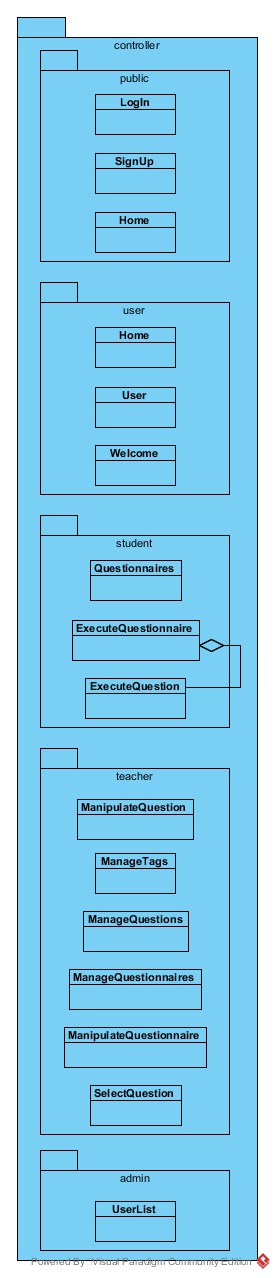
\includegraphics[scale=4, max width=\textwidth, max height=\myheight]{../img/diagrammiClassi/client/controller.png}
		\caption{Diagramma package - client::controller}
	\end{figure}
\end{center}\subsubsection{client::controller::public}
È il package che contiene tutte le classi che costituiscono i controller della porzione pubblica di un client. Ogni componente si occupa della gestione di una particolare porzione dell'interfaccia di un utente non autenticato che verrà successivamente visualizzata nella corrispondente view.\begin{center}
	\begin{figure}[H]
		\centering 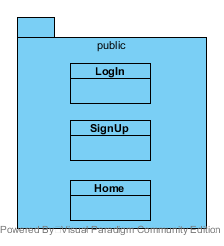
\includegraphics[scale=4, max width=\textwidth, max height=\myheight]{../img/diagrammiClassi/client/controller/public.png}
		\caption{Diagramma package - client::controller::public}
	\end{figure}
\end{center}\hypertarget{client::controller::public::LogIn}{}
\subsubsubsection[LogIn]{client::controller::public::LogIn}

\begin{figure}[H]
	\centering
	%\begin{turn}{90}
	\begin{tikzpicture}
	\umlclass{client::controller::public::LogIn} {--location : Object\\--rootScope : Object\\--scope : Object\\--sessionService : SessionService\\--check : Check\\--userService : UserService\\--cookies : Object\\--error : Error\\--userName : String\\--password : String}{+LogIn(check : Check, cookies : Object, location : Object, userService : UserService, \\ rootScope : Object, scope : Object, sessionService : SessionService)\\+submit() : void\\+checkUserName() : boolean\\+checkPassword() : boolean\\+getError() : Error\\+getUserName() : String\\+getPassword() : String\\+setError(error : Error) : void\\+setUserName(userName : String) : void\\+setPassword(password : String) : void}
	\end{tikzpicture}
	%\end{turn}
	\caption{Diagramma classe - client::controller::public::LogIn}
\end{figure}\begin{description}
\item[Descrizione] \hfill \\
Classe che gestisce le operazioni e la logica applicativa riguardante la pagina di autenticazione sul client
\item[Utilizzo] \hfill \\
Viene utilizzata per generare la pagina di autenticazione all’applicazione. Prima della creazione della view viene effettuato un controllo sull’esistenza di una sessione utente. In caso positivo il controller si occuperà di visualizzare la home dell'utente loggato, altrimenti si procederà alla pagina di Login predefinita.
\item[Relazioni con altre classi] \hfill \\
\vspace{-7mm}
\begin{description}
	\item[\hyperlink{client::util::Check}{client::util::Check}] \hfill \\
	Relazione uscente, campo dati che rappresenta un oggetto Check
	\item[\hyperlink{client::model::service::UserService}{client::model::service::UserService}] \hfill \\
	Relazione uscente, campo dati che rappresenta un oggetto UserService
	\item[\hyperlink{client::model::data::Error}{client::model::data::Error}] \hfill \\
	Relazione uscente, campo dati che rappresenta un oggetto Error
	\item[\hyperlink{client::model::service::SessionService}{client::model::service::SessionService}] \hfill \\
	Relazione uscente, campo dati che rappresenta un oggetto SessionService
\end{description}

\item[Attributi] \hfill \\
\vspace{-7mm}
\begin{itemize}
	\item location : Object $\rightarrow$ oggetto di angular che analizza l'URL nella barra degli indirizzi del browser e lo rende disponibile all'applicazione
	\item rootScope : Object $\rightarrow$ oggetto di angular che identifica l’elemento con attributo ng-app
	\item scope : Object $\rightarrow$ oggetto di angular che fa riferimento ad una porzione di model di pertinenza di uno specifico controller
	\item sessionService : SessionService $\rightarrow$ campo dati che rappresenta un oggetto SessionService
	\item check : Check $\rightarrow$ campo dati che rappresenta un oggetto Check
	\item userService : UserService $\rightarrow$ campo dati che rappresenta un oggetto UserService
	\item cookies : Object $\rightarrow$ oggetto di angular che permette di manipolare i cookies
	\item error : Error $\rightarrow$ campo dati che rappresenta un oggetto Error
	\item userName : String $\rightarrow$ rappresenta il campo userName nella View
	\item password : String $\rightarrow$ rappresenta il campo password nella view
\end{itemize}

\item[Metodi] \hfill \\
\vspace{-7mm}
\begin{itemize}
	\item LogIn(check : Check, cookies : Object, location : Object, userService : UserService, rootScope : Object, scope : Object, sessionService : SessionService) $\rightarrow$ costruttore della classe\begin{itemize}
		\item check $\rightarrow$ campo dati che rappresenta un oggetto Check
		\item cookies $\rightarrow$ oggetto di angular che permette di manipolare i cookies
		\item location $\rightarrow$ oggetto di angular che analizza l'URL nella barra degli indirizzi del browser e lo rende disponibile all'applicazione
		\item userService $\rightarrow$ campo dati che rappresenta un oggetto UserService
		\item rootScope $\rightarrow$ oggetto di angular che identifica l’elemento con attributo ng-app
		\item scope $\rightarrow$ oggetto di angular che fa riferimento ad una porzione di model di pertinenza di uno specifico controller
		\item sessionService $\rightarrow$ campo dati che rappresenta un oggetto SessionService
	\end{itemize}
	
	\item submit() : void $\rightarrow$ invia lo username e la password dell'utente al servizio che effettua l'autenticazione istanziando una nuova sessione
	\item checkUserName() : boolean $\rightarrow$ metodo che controlla che l'userName inserito rispetti alcuni parametri richiamando il relativo metodo nella classe Check
	\item checkPassword() : boolean $\rightarrow$ metodo che controlla che la password inserita rispetti alcuni parametri richiamando il relativo metodo nella classe Check
	\item getError() : Error $\rightarrow$ metodo getter
	\item getUserName() : String $\rightarrow$ metodo getter
	\item getPassword() : String $\rightarrow$ metodo getter
	\item setError(error : Error) : void $\rightarrow$ metodo setter\begin{itemize}
		\item error $\rightarrow$ campo dati che rappresenta un oggetto Error
	\end{itemize}
	
	\item setUserName(userName : String) : void $\rightarrow$ metodo setter\begin{itemize}
		\item userName $\rightarrow$ rappresenta il campo userName nella View
	\end{itemize}
	
	\item setPassword(password : String) : void $\rightarrow$ metodo setter\begin{itemize}
		\item password $\rightarrow$ rappresenta il campo password nella view
	\end{itemize}
	
\end{itemize}

\end{description}

\vspace{0.5cm}
\hypertarget{client::controller::public::SignUp}{}
\subsubsubsection[SignUp]{client::controller::public::SignUp}
\begin{figure}[H]
	\centering
	\begin{tikzpicture}
	\umlclass{client::controller::public::SignUp} {--location : Object\\--rootScope : Object\\--scope : Object\\--sessionService : SessionService\\--userService : UserService\\--cookies : Object\\--check : Check\\--error	 : Error	\\--userName : String\\--password : String\\--fullName : String\\--repeatPassword : String}{+SignUp(check : Check, cookies : Object, location : Object, scope : Object, rootScope : Object, \\ sessionService : SessionService, userService : UserService)\\+checkPassword() : boolean\\+checkRepeatPassword() : boolean\\+checkUserName() : boolean\\+submit() : void\\+checkFullName() : boolean\\+getError	() : Error	\\+getUserName() : String\\+getPassword() : String\\+getFullName() : String\\+getRepeatPassword() : String\\+setError	(error	 : Error	) : void\\+setUserName(userName : String) : void\\+setPassword(password : String) : void\\+setFullName(fullName : String) : void\\+setRepeatPassword(repeatPassword : String) : void}
	\end{tikzpicture}
	\caption{Diagramma classe - client::controller::public::SignUp}
\end{figure}\begin{description}
\item[Descrizione] \hfill \\
Classe che gestisce le operazioni e la logica applicativa riguardante la pagina di Registrazione sul client
\item[Utilizzo] \hfill \\
Deve visualizzare campi per l’inserimento della mail, password, nome e cognome. Deve poter gestire l'eventuale caso di errore se la mail dello studente è già presente nel sistema. Inoltre deve poter gestire il caso in cui di la password dello studente non rispetta i parametri prestabiliti 
\item[Relazioni con altre classi] \hfill \\
\vspace{-7mm}
\begin{description}
	\item[\hyperlink{client::util::Check}{client::util::Check}] \hfill \\
	Relazione uscente, campo dati che rappresenta un oggetto Check
	\item[\hyperlink{client::model::data::Error}{client::model::data::Error}] \hfill \\
	Relazione uscente, oggetto che rappresenta un errore da visualizzare all'utente
	\item[\hyperlink{client::model::service::SessionService}{client::model::service::SessionService}] \hfill \\
	Relazione uscente, campo dati che rappresenta un oggetto SessionService
	\item[\hyperlink{client::model::service::UserService}{client::model::service::UserService}] \hfill \\
	Relazione uscente, campo dati che rappresenta un oggetto UserService
\end{description}

\item[Attributi] \hfill \\
\vspace{-7mm}
\begin{itemize}
	\item location : Object $\rightarrow$ oggetto di angular che analizza l'URL nella barra degli indirizzi del browser e lo rende disponibile all'applicazione
	\item rootScope : Object $\rightarrow$ oggetto di angular che identifica l’elemento con attributo ng-app
	\item scope : Object $\rightarrow$ oggetto di angular che fa riferimento ad una porzione di model di pertinenza di uno specifico controller
	\item sessionService : SessionService $\rightarrow$ campo dati che rappresenta un oggetto SessionService
	\item userService : UserService $\rightarrow$ campo dati che rappresenta un oggetto UserService
	\item cookies : Object $\rightarrow$ oggetto di angular che permette di manipolare i cookies
	\item check : Check $\rightarrow$ campo dati che rappresenta un oggetto Check
	\item error	 : Error	 $\rightarrow$ oggetto che rappresenta un errore da visualizzare all'utente
	\item userName : String $\rightarrow$ rappresenta il campo userName nella View
	\item password : String $\rightarrow$ rappresenta il campo password nella View
	\item fullName : String $\rightarrow$ rappresenta il campo fullName nella View
	\item repeatPassword : String $\rightarrow$ rappresenta il campo repeatPassword nella View
\end{itemize}

\item[Metodi] \hfill \\
\vspace{-7mm}
\begin{itemize}
	\item SignUp(check : Check, cookies : Object, location : Object, scope : Object, rootScope : Object, sessionService : SessionService, userService : UserService) $\rightarrow$ costruttore della classe\begin{itemize}
		\item check $\rightarrow$ campo dati che rappresenta un oggetto Check
		\item cookies $\rightarrow$ oggetto di angular che permette di manipolare i cookies
		\item location $\rightarrow$ oggetto di angular che analizza l'URL nella barra degli indirizzi del browser e lo rende disponibile all'applicazione
		\item scope $\rightarrow$ oggetto di angular che fa riferimento ad una porzione di model di pertinenza di uno specifico controller
		\item rootScope $\rightarrow$ oggetto di angular che identifica l’elemento con attributo ng-app
		\item sessionService $\rightarrow$ campo dati che rappresenta un oggetto SessionService
		\item userService $\rightarrow$ campo dati che rappresenta un oggetto UserService
	\end{itemize}
	
	\item checkPassword() : boolean $\rightarrow$ controlla se la password inserita ha i requisiti minimi richiamando il relativo metodo nella classe Check
	\item checkRepeatPassword() : boolean $\rightarrow$ controlla se la password è uguale a quella inserita nel campo "Ripeti password"
	\item checkUserName() : boolean $\rightarrow$ controlla su lo username ha i requisiti minimi richiamando il relativo metodo nella classe Check
	\item submit() : void $\rightarrow$ invia i dati dell'utente al servizio che effettua la registrazione
	\item checkFullName() : boolean $\rightarrow$ controlla se il nome inserito ha i requisiti minimi richiamando il relativo metodo nella classe Check
	\item getError	() : Error	 $\rightarrow$ metodo getter
	\item getUserName() : String $\rightarrow$ metodo getter
	\item getPassword() : String $\rightarrow$ metodo getter
	\item getFullName() : String $\rightarrow$ metodo getter
	\item getRepeatPassword() : String $\rightarrow$ metodo getter
	\item setError	(error	 : Error	) : void $\rightarrow$ metodo setter\begin{itemize}
		\item error	 $\rightarrow$ oggetto che rappresenta un errore da visualizzare all'utente
	\end{itemize}
	
	\item setUserName(userName : String) : void $\rightarrow$ metodo setter\begin{itemize}
		\item userName $\rightarrow$ rappresenta il campo userName nella View
	\end{itemize}
	
	\item setPassword(password : String) : void $\rightarrow$ metodo setter\begin{itemize}
		\item password $\rightarrow$ rappresenta il campo password nella View
	\end{itemize}
	
	\item setFullName(fullName : String) : void $\rightarrow$ metodo setter\begin{itemize}
		\item fullName $\rightarrow$ rappresenta il campo fullName nella View
	\end{itemize}
	
	\item setRepeatPassword(repeatPassword : String) : void $\rightarrow$ metodo setter\begin{itemize}
		\item repeatPassword $\rightarrow$ rappresenta il campo repeatPassword nella View
	\end{itemize}
	
\end{itemize}

\end{description}

\vspace{0.5cm}
\hypertarget{client::controller::public::Home}{}
\subsubsubsection[Home]{client::controller::public::Home}
\begin{figure}[H]
	\centering
	\begin{tikzpicture}
	\umlclass{client::controller::public::Home} {--location : Object\\--scope : Object\\--cookies : Object\\--rootScope : Object\\--userService : UserService}{+Home(rootScope : Object, cookies : Object, scope : Object, location : Object, \\ userService : UserService)\\+checkLogged() : void\\+urlPath() : void}
	\end{tikzpicture}
	\caption{Diagramma classe - client::controller::public::Home}
\end{figure}\begin{description}
\item[Descrizione] \hfill \\
Classe che gestisce le operazioni e la logica applicativa riguardante la status bar e la slide bar
\item[Relazioni con altre classi] \hfill \\
\vspace{-7mm}
\begin{description}
	\item[\hyperlink{client::model::service::UserService}{client::model::service::UserService}] \hfill \\
	Relazione uscente, campo dati che rappresenta un oggetto UserService
\end{description}

\item[Attributi] \hfill \\
\vspace{-7mm}
\begin{itemize}
	\item location : Object $\rightarrow$ oggetto di angular che analizza l'URL nella barra degli indirizzi del browser e lo rende disponibile all'applicazione
	\item scope : Object $\rightarrow$ oggetto di angular che fa riferimento ad una porzione di model di pertinenza di uno specifico controller
	\item cookies : Object $\rightarrow$ oggetto di angular che permette di manipolare i cookies
	\item rootScope : Object $\rightarrow$ oggetto di angular che identifica l’elemento con attributo ng-app
	\item userService : UserService $\rightarrow$ campo dati che rappresenta un oggetto UserService
\end{itemize}

\item[Metodi] \hfill \\
\vspace{-7mm}
\begin{itemize}
	\item Home(rootScope : Object, cookies : Object, scope : Object, location : Object, userService : UserService) $\rightarrow$ costruttore della classe\begin{itemize}
		\item rootScope $\rightarrow$ oggetto di angular che identifica l’elemento con attributo ng-app
		\item cookies $\rightarrow$ oggetto di angular che permette di manipolare i cookies
		\item scope $\rightarrow$ oggetto di angular che fa riferimento ad una porzione di model di pertinenza di uno specifico controller
		\item location $\rightarrow$ oggetto di angular che analizza l'URL nella barra degli indirizzi del browser e lo rende disponibile all'applicazione
		\item userService $\rightarrow$ campo dati che rappresenta un oggetto UserService
	\end{itemize}
	
	\item checkLogged() : void $\rightarrow$ controlla se l'utente è già loggato controllando i cookies di sessione
	\item urlPath() : void $\rightarrow$ restituisce l'array contenente ogni parte del path dell'url
\end{itemize}

\end{description}

\vspace{0.5cm}
\subsubsection{client::controller::student}
È il package che contiene tutte le classi che costituiscono i controller della porzione client per uno studente. Ogni componente si occupa della gestione di una particolare porzione dell'interfaccia di uno studente.\begin{center}
	\begin{figure}[H]
		\centering 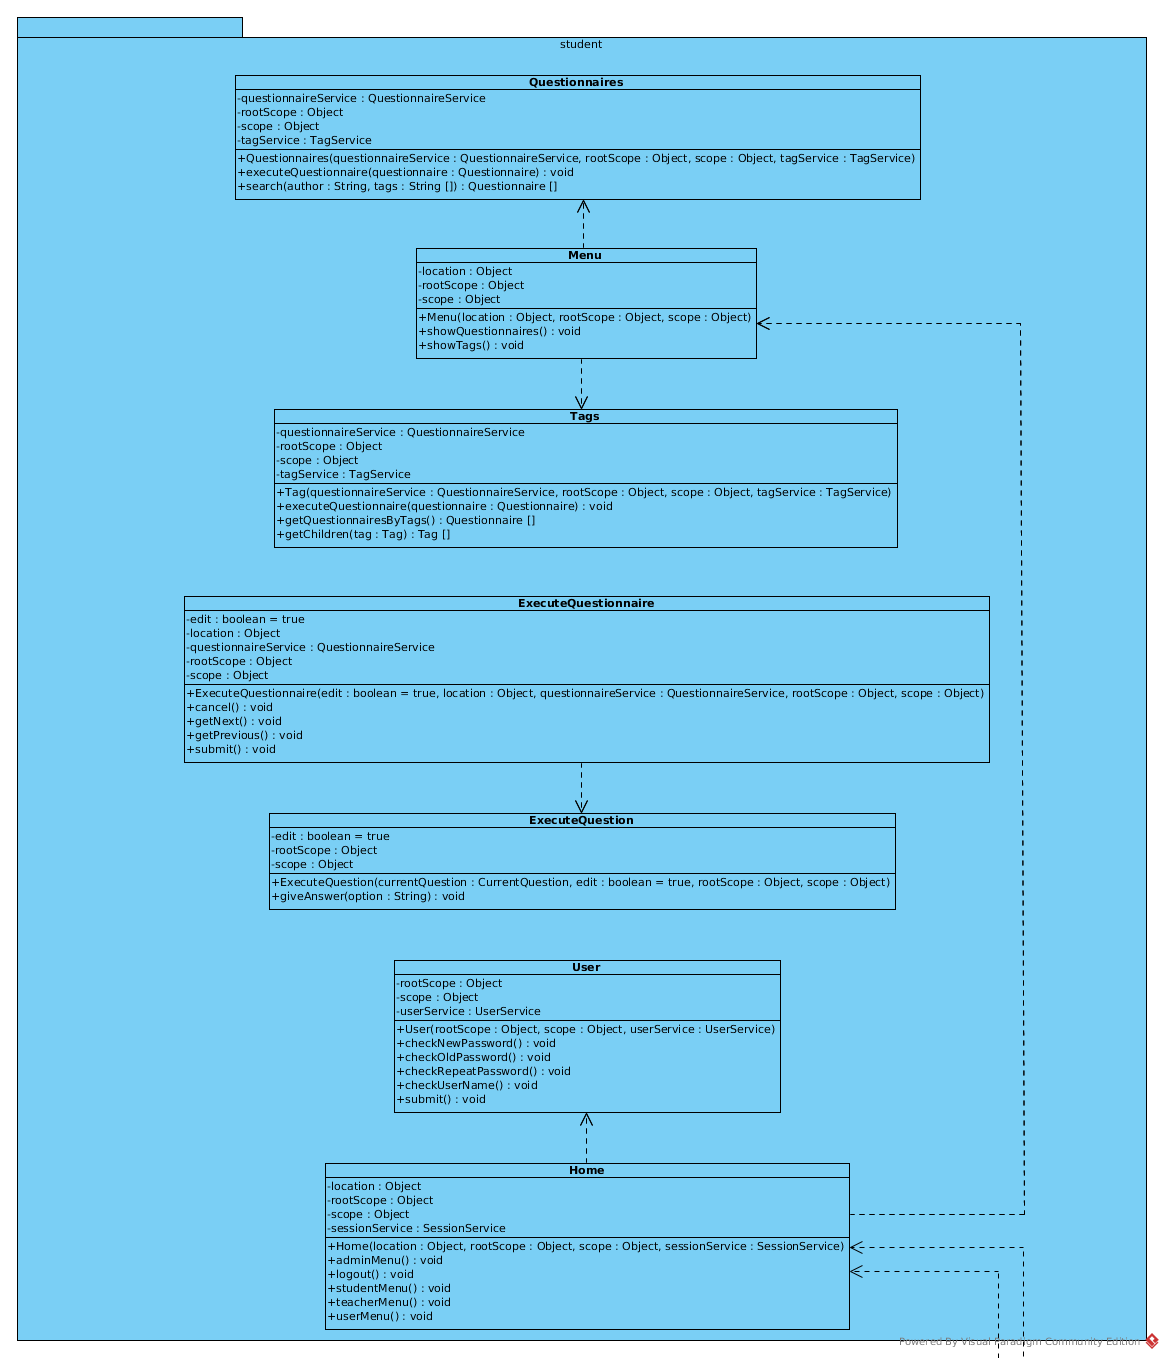
\includegraphics[scale=4, max width=\textwidth, max height=\myheight]{../img/diagrammiClassi/client/controller/student.png}
		\caption{Diagramma package - client::controller::student}
	\end{figure}
\end{center}\hypertarget{client::controller::student::Questionnaires}{}
\subsubsubsection[Questionnaires]{client::controller::student::Questionnaires}
\begin{figure}[H]
	\centering
	\begin{tikzpicture}
	\umlclass{client::controller::student::Questionnaires} {--scope : Object\\--questionnaireService : QuestionnaireService\\--tagService : TagService\\--questList : Questionnaire[]\\--userService : UserService\\--titleSearch : String\\--tagSearch : String\\--authorSearch : String\\--myOrderBy : String\\--location : Object}{+Questionnaires(userService : UserService, questionnaireService : QuestionnaireService, \\ rootScope : Object, scope : Object, tagService : TagService)\\+executeQuestionnaire(questID : integer) : void\\+submit() : void\\+setMyOrderBy(myOrderBy : String) : void\\+setAuthorSearch(authorSearch : String) : void\\+setQuestList(questList : Questionnaire[]) : void\\+setTagSearch(tagSearch : String) : void\\+setTitleSearch(titleSearch : String) : void\\+getAuthorSearch() : String\\+getQuestList() : Questionnaire []\\+getTagSearch() : String\\+getTitleSearch() : String\\+getMyOrderBy() : String}
	\end{tikzpicture}
	\caption{Diagramma classe - client::controller::student::Questionnaires}
\end{figure}\begin{description}
\item[Descrizione] \hfill \\
Classe che si occupa della ricerca di un questionario da parte di uno studente e dell'eventuale gestione di una richiesta di esecuzione di un questionario
\item[Utilizzo] \hfill \\
Si occupa di gestire la ricerca di un questionario e di permettere ad uno studente di navigare tra i questionari presenti nel sistema per sceglierne eventualmente uno da eseguire
\item[Relazioni con altre classi] \hfill \\
\vspace{-7mm}
\begin{description}
	\item[\hyperlink{client::model::data::Questionnaire}{client::model::data::Questionnaire}] \hfill \\
	Relazione uscente, lista di questionari
	\item[\hyperlink{client::model::service::UserService}{client::model::service::UserService}] \hfill \\
	Relazione uscente, campo dati che rappresenta un oggetto UserService
	\item[\hyperlink{client::model::service::TagService}{client::model::service::TagService}] \hfill \\
	Relazione uscente, campo dati che rappresenta un oggetto TagService
	\item[\hyperlink{client::model::service::QuestionnaireService}{client::model::service::QuestionnaireService}] \hfill \\
	Relazione uscente, campo dati che rappresenta un oggetto QuestionnaireService
\end{description}

\item[Attributi] \hfill \\
\vspace{-7mm}
\begin{itemize}
	\item scope : Object $\rightarrow$ oggetto di angular che fa riferimento ad una porzione di model di pertinenza di uno specifico controller
	\item questionnaireService : QuestionnaireService $\rightarrow$ campo dati che rappresenta un oggetto QuestionnaireService
	\item tagService : TagService $\rightarrow$ campo dati che rappresenta un oggetto TagService
	\item questList : Questionnaire[] $\rightarrow$ lista di questionari
	\item userService : UserService $\rightarrow$ campo dati che rappresenta un oggetto UserService
	\item titleSearch : String $\rightarrow$ rappresenta il campo titleSearch nella View
	\item tagSearch : String $\rightarrow$ rappresenta il campo tagSearch nella View
	\item authorSearch : String $\rightarrow$ rappresenta il campo authorSearch nella View
	\item myOrderBy : String $\rightarrow$ stringa che si riferisce al campo per cui ordinare i questionari
	\item location : Object $\rightarrow$ oggetto di angular che analizza l'URL nella barra degli indirizzi del browser e lo rende disponibile all'applicazione
\end{itemize}

\item[Metodi] \hfill \\
\vspace{-7mm}
\begin{itemize}
	\item Questionnaires(userService : UserService, questionnaireService : QuestionnaireService, rootScope : Object, scope : Object, tagService : TagService) $\rightarrow$ costruttore della classe\begin{itemize}
		\item userService $\rightarrow$ campo dati che rappresenta un oggetto UserService
		\item questionnaireService $\rightarrow$ campo dati che rappresenta un oggetto QuestionnaireService
		\item rootScope $\rightarrow$ oggetto di angular che identifica l’elemento con attributo ng-app
		\item scope $\rightarrow$ oggetto di angular che fa riferimento ad una porzione di model di pertinenza di uno specifico controller
		\item tagService $\rightarrow$ campo dati che rappresenta un oggetto TagService 
	\end{itemize}
	
	\item executeQuestionnaire(questID : integer) : void $\rightarrow$ permette di eseguire il questionario passato come parametro caricandone la relativa view\begin{itemize}
		\item questID $\rightarrow$ contiene l'ID del questionario da eseguire
	\end{itemize}
	
	\item submit() : void $\rightarrow$ permette di ricercare questionari filtrandoli in base ad autore, titolo e argomenti, richiamando gli opportuni servizi che mandano la richiesta al server
	\item setMyOrderBy(myOrderBy : String) : void $\rightarrow$ metodo setter\begin{itemize}
		\item myOrderBy $\rightarrow$ stringa che si riferisce al campo per cui ordinare i questionari
	\end{itemize}
	
	\item setAuthorSearch(authorSearch : String) : void $\rightarrow$ metodo setter\begin{itemize}
		\item authorSearch $\rightarrow$ rappresenta il campo authorSearch nella View
	\end{itemize}
	
	\item setQuestList(questList : Questionnaire[]) : void $\rightarrow$ metodo setter\begin{itemize}
		\item questList $\rightarrow$ lista di questionari
	\end{itemize}
	
	\item setTagSearch(tagSearch : String) : void $\rightarrow$ metodo setter\begin{itemize}
		\item tagSearch $\rightarrow$ rappresenta il campo tagSearch nella View
	\end{itemize}
	
	\item setTitleSearch(titleSearch : String) : void $\rightarrow$ metodo setter\begin{itemize}
		\item titleSearch $\rightarrow$ rappresenta il campo titleSearch nella View
	\end{itemize}
	
	\item getAuthorSearch() : String $\rightarrow$ metodo getter
	\item getQuestList() : Questionnaire [] $\rightarrow$ metodo getter
	\item getTagSearch() : String $\rightarrow$ metodo getter
	\item getTitleSearch() : String $\rightarrow$ metodo getter
	\item getMyOrderBy() : String $\rightarrow$ metodo getter
\end{itemize}

\end{description}

\vspace{0.5cm}
\hypertarget{client::controller::student::ExecuteQuestionnaire}{}
\subsubsubsection[ExecuteQuestionnaire]{client::controller::student::ExecuteQuestionnaire}
\begin{figure}[H]
	\centering
	\begin{tikzpicture}
	\umlclass{client::controller::student::ExecuteQuestionnaire} {--questionnaireService : QuestionnaireService\\--scope : Object\\--questionnaire : CurrentQuestionnaire\\--currentQuestion : ExecuteQuestion\\--util : Util\\--q : Object}{+ExecuteQuestionnaire(location : Object, questionnaireService : QuestionnaireService, \\ rootScope : Object, scope : Object, edit : boolean)\\+getNext() : void\\+getPrevious() : void\\+submit() : void}
	\end{tikzpicture}
	\caption{Diagramma classe - client::controller::student::ExecuteQuestionnaire}
\end{figure}\begin{description}
\item[Descrizione] \hfill \\
La classe che controlla esecuzione del questionario 
\item[Utilizzo] \hfill \\
Viene chiamata quando uno studente comincia a rispondere ad un questionario. Lo studente non è obbligato a rispondere alle domande una dopo l'altra, ha la possibilità di poter tornare su domande che in precedenza non aveva risposto. Solo dopo il submit che il questionario si considera completato
\item[Relazioni con altre classi] \hfill \\
\vspace{-7mm}
\begin{description}
	\item[\hyperlink{client::model::data::CurrentQuestionnaire}{client::model::data::CurrentQuestionnaire}] \hfill \\
	Relazione uscente, istanza del questionario in esecuzione
	\item[\hyperlink{client::controller::student::ExecuteQuestion}{client::controller::student::ExecuteQuestion}] \hfill \\
	Relazione uscente, oggetto controller di ExecuteQuestion che gestisce la domanda corrente
	\item[\hyperlink{client::util::Util}{client::util::Util}] \hfill \\
	Relazione uscente, campo dati che rappresenta un oggetto Util
	\item[\hyperlink{client::model::service::QuestionnaireService}{client::model::service::QuestionnaireService}] \hfill \\
	Relazione uscente, campo dati che rappresenta un oggetto QuestionnaireService
\end{description}

\item[Attributi] \hfill \\
\vspace{-7mm}
\begin{itemize}
	\item questionnaireService : QuestionnaireService $\rightarrow$ campo dati che rappresenta un oggetto QuestionnaireService
	\item scope : Object $\rightarrow$ oggetto di angular che fa riferimento ad una porzione di model di pertinenza di uno specifico controller
	\item questionnaire : CurrentQuestionnaire $\rightarrow$ istanza del questionario in esecuzione
	\item currentQuestion : ExecuteQuestion $\rightarrow$ oggetto controller di ExecuteQuestion che gestisce la domanda corrente
	\item util : Util $\rightarrow$ campo dati che rappresenta un oggetto Util
	\item q : Object $\rightarrow$ oggetto di angular che permette di eseguire funzioni asincrone
\end{itemize}

\item[Metodi] \hfill \\
\vspace{-7mm}
\begin{itemize}
	\item ExecuteQuestionnaire(location : Object, questionnaireService : QuestionnaireService, rootScope : Object, scope : Object, edit : boolean) $\rightarrow$ costruttore della classe\begin{itemize}
		\item location $\rightarrow$ oggetto di angular che analizza l'URL nella barra degli indirizzi del browser e lo rende disponibile all'applicazione
		\item questionnaireService $\rightarrow$ campo dati che rappresenta un oggetto QuestionnaireService
		\item rootScope $\rightarrow$ oggetto di angular che identifica l’elemento con attributo ng-app
		\item scope $\rightarrow$ oggetto di angular che fa riferimento ad una porzione di model di pertinenza di uno specifico controller
		\item edit $\rightarrow$ indica se esecuzione del questionario è in modalità read-only. Ovvero se variabile è true allora si possono cambiare le risposte alle domande, altrimenti si può solo visualizzare il questionario senza poter cambiare le risposte già selezionate 
	\end{itemize}
	
	\item getNext() : void $\rightarrow$ carica la prossima domanda in executeQuestion
	\item getPrevious() : void $\rightarrow$ carica a domanda precedente in executeQuestion
	\item submit() : void $\rightarrow$ controlla che tutte le risposte siano state date, in caso positivo richiama il metodo per ottenere i risultati e li visualizza, altrimenti visualizza un messaggio di errore
\end{itemize}

\end{description}

\vspace{0.5cm}
\hypertarget{client::controller::student::ExecuteQuestion}{}
\subsubsubsection[ExecuteQuestion]{client::controller::student::ExecuteQuestion}
\begin{figure}[H]
	\centering
	\begin{tikzpicture}
	\umlclass{client::controller::student::ExecuteQuestion} {--scope : Object\\--interpolate : Object\\--sce : Object}{+ExecuteQuestion(currentQuestion : CurrentQuestion, edit : boolean, rootScope : Object, \\ scope : Object)\\+giveAnswer(option : String) : void\\+setCurrentQuestion(currentQuestion : currentQuesion) : void}
	\end{tikzpicture}
	\caption{Diagramma classe - client::controller::student::ExecuteQuestion}
\end{figure}\begin{description}
\item[Descrizione] \hfill \\
La classe che controlla l'esecuzione di una domanda 
\item[Utilizzo] \hfill \\
Viene chiamata per dare la possibilità ad uno studente di eseguire una specifica domanda all'interno di un questionario in esecuzione
\item[Relazioni con altre classi] \hfill \\
\vspace{-7mm}
\begin{description}
	\item[\hyperlink{client::controller::student::ExecuteQuestionnaire}{client::controller::student::ExecuteQuestionnaire}] \hfill \\
	Relazione entrante, oggetto controller di ExecuteQuestion che gestisce la domanda corrente
\end{description}

\item[Attributi] \hfill \\
\vspace{-7mm}
\begin{itemize}
	\item scope : Object $\rightarrow$ oggetto di angular che fa riferimento ad una porzione di model di pertinenza di uno specifico controller
	\item interpolate : Object $\rightarrow$ oggetto di angular che permette l'interpolazione di stringhe
	\item sce : Object $\rightarrow$ oggetto di angular che permette il trattamento di stringhe in alcuni contesti dove richiedono di essere marcate come sicure
\end{itemize}

\item[Metodi] \hfill \\
\vspace{-7mm}
\begin{itemize}
	\item ExecuteQuestion(currentQuestion : CurrentQuestion, edit : boolean, rootScope : Object, scope : Object) $\rightarrow$ costruttore della classe\begin{itemize}
		\item currentQuestion $\rightarrow$ contiene la domanda corrente da eseguire 
		\item edit $\rightarrow$ true - si può modificare, false - no 
		\item rootScope $\rightarrow$ oggetto di angular che identifica l’elemento con attributo ng-app
		\item scope $\rightarrow$ oggetto di angular che fa riferimento ad una porzione di model di pertinenza di uno specifico controller
	\end{itemize}
	
	\item giveAnswer(option : String) : void $\rightarrow$ metodo che viene chiamato ogni volta che viene modificata la risposta data e la memorizza in currentQuestion\begin{itemize}
		\item option $\rightarrow$ contiene la risposta alla domanda  data dall'utente 
	\end{itemize}
	
	\item setCurrentQuestion(currentQuestion : currentQuesion) : void $\rightarrow$ metodo che cambia la currentQuestion in esecuzione. Questo metodo viene chiamato da executeQuestionnaire quando viene selezionata la domanda successiva o precedente\begin{itemize}
		\item currentQuestion $\rightarrow$ currentQuestion da caricare in esecuzione
	\end{itemize}
	
\end{itemize}

\end{description}

\vspace{0.5cm}
\subsubsection{client::controller::teacher}
È il package che contiene tutte le classi che costituiscono i controller della porzione client per un docente. Ogni componente si occupa della gestione di una particolare porzione dell'interfaccia di un docente.\begin{center}
	\begin{figure}[H]
		\centering 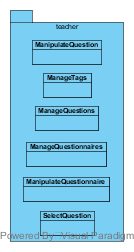
\includegraphics[scale=4, max width=\textwidth, max height=\myheight]{../img/diagrammiClassi/client/controller/teacher.png}
		\caption{Diagramma package - client::controller::teacher}
	\end{figure}
\end{center}\hypertarget{client::controller::teacher::ManipulateQuestion}{}
\subsubsubsection[ManipulateQuestion]{client::controller::teacher::ManipulateQuestion}
\begin{figure}[H]
	\centering
	\begin{tikzpicture}
	\umlclass{client::controller::teacher::ManipulateQuestion} {--question : Question \\--rootScope : Object\\--questionService : QuestionService\\--scope : Object\\--tagService : TagService\\--location : Object\\--qml : QML\\--error : Error\\--edit : boolean\\--editor : SimpleMDE\\--tagsInput : String\\--tags : Tag []\\--editorBuilder : Editor}{+ManipulateQuestion(question : Question, questionService : QuestionService, scope : Object, \\ rootScope : Object)\\+submit() : void\\+getError() : Error\\+setError(error : Error) : void\\+getEditor() : SimpleMDE\\+getEdit() : boolean\\+getQuestion() : Question \\+getTags() : Tag []\\+getTagsInput() : String\\+setEditor(editor : SimpleMDE) : void\\+setEdit(edit : boolean) : void\\+setQuestion(question : Question ) : void\\+setTags(tags : Tag []) : void\\+setTagsInput(tagsInput : String) : void}
	\end{tikzpicture}
	\caption{Diagramma classe - client::controller::teacher::ManipulateQuestion}
\end{figure}\begin{description}
\item[Descrizione] \hfill \\
Classe che si occupa della gestione della domanda lato docente
\item[Utilizzo] \hfill \\
Viene richiamata quando un docente vuole aggiungere,  modificare o eliminare una domanda
\item[Relazioni con altre classi] \hfill \\
\vspace{-7mm}
\begin{description}
	\item[\hyperlink{client::model::data::Question}{client::model::data::Question}] \hfill \\
	Relazione uscente, oggetto che rappresenta una singola domanda
	\item[\hyperlink{client::model::service::TagService}{client::model::service::TagService}] \hfill \\
	Relazione uscente, campo dati che rappresenta un oggetto TagService
	\item[\hyperlink{client::util::QML}{client::util::QML}] \hfill \\
	Relazione uscente, campo dati che rappresenta un oggetto QML
	\item[\hyperlink{client::model::data::Error}{client::model::data::Error}] \hfill \\
	Relazione uscente, campo dati che rappresenta un oggetto Error
	\item[\hyperlink{client::model::data::Tag}{client::model::data::Tag}] \hfill \\
	Relazione uscente, argomenti che compaiono nei suggerimenti
	\item[\hyperlink{client::model::service::QuestionService}{client::model::service::QuestionService}] \hfill \\
	Relazione uscente, campo dati che rappresenta un oggetto QuestionService
	\item[\hyperlink{client::util::Editor}{client::util::Editor}] \hfill \\
	Relazione uscente, campo dati che rappresenta un oggetto Editor
\end{description}

\item[Attributi] \hfill \\
\vspace{-7mm}
\begin{itemize}
	\item question : Question  $\rightarrow$ oggetto che rappresenta una singola domanda
	\item rootScope : Object $\rightarrow$ oggetto di angular che identifica l’elemento con attributo ng-app
	\item questionService : QuestionService $\rightarrow$ campo dati che rappresenta un oggetto QuestionService
	\item scope : Object $\rightarrow$ oggetto di angular che fa riferimento ad una porzione di model di pertinenza di uno specifico controller
	\item tagService : TagService $\rightarrow$ campo dati che rappresenta un oggetto TagService
	\item location : Object $\rightarrow$ oggetto di angular che analizza l'URL nella barra degli indirizzi del browser e lo rende disponibile all'applicazione
	\item qml : QML $\rightarrow$ campo dati che rappresenta un oggetto QML
	\item error : Error $\rightarrow$ campo dati che rappresenta un oggetto Error
	\item edit : boolean $\rightarrow$ indica se la domanda corrente è nuova o se si sta modificando una già creata
	\item editor : SimpleMDE $\rightarrow$ oggetto che rappreseta l'editor per manipolare la domanda
	\item tagsInput : String $\rightarrow$ rappresenta il campo tagsInput nella View
	\item tags : Tag [] $\rightarrow$ argomenti che compaiono nei suggerimenti
	\item editorBuilder : Editor $\rightarrow$ campo dati che rappresenta un oggetto Editor
\end{itemize}

\item[Metodi] \hfill \\
\vspace{-7mm}
\begin{itemize}
	\item ManipulateQuestion(question : Question, questionService : QuestionService, scope : Object, rootScope : Object) $\rightarrow$ costruttore della classe\begin{itemize}
		\item question $\rightarrow$ contiene il riferimento verso il modello delle domande 
		\item questionService $\rightarrow$ campo dati che rappresenta un oggetto QuestionService
		\item scope $\rightarrow$ oggetto di angular che fa riferimento ad una porzione di model di pertinenza di uno specifico controller
		\item rootScope $\rightarrow$ oggetto di angular che identifica l’elemento con attributo ng-app
	\end{itemize}
	
	\item submit() : void $\rightarrow$ dopo aver controllato la validità del titolo, tags e QML inseriti, invia i dati al servizio che si occupa di inserire la domanda nel sistema
	\item getError() : Error $\rightarrow$ metodo getter
	\item setError(error : Error) : void $\rightarrow$ metodo setter\begin{itemize}
		\item error $\rightarrow$ campo dati che rappresenta un oggetto Error
	\end{itemize}
	
	\item getEditor() : SimpleMDE $\rightarrow$ metodo getter
	\item getEdit() : boolean $\rightarrow$ metodo getter
	\item getQuestion() : Question  $\rightarrow$ metodo getter
	\item getTags() : Tag [] $\rightarrow$ metodo getter
	\item getTagsInput() : String $\rightarrow$ metodo getter
	\item setEditor(editor : SimpleMDE) : void $\rightarrow$ metodo setter\begin{itemize}
		\item editor $\rightarrow$ oggetto che rappreseta l'editor per manipolare la domanda
	\end{itemize}
	
	\item setEdit(edit : boolean) : void $\rightarrow$ metodo setter\begin{itemize}
		\item edit $\rightarrow$ indica se la domanda corrente è nuova o se si sta modificando una già creata
	\end{itemize}
	
	\item setQuestion(question : Question ) : void $\rightarrow$ metodo setter\begin{itemize}
		\item question $\rightarrow$ oggetto che rappresenta una singola domanda
	\end{itemize}
	
	\item setTags(tags : Tag []) : void $\rightarrow$ metodo setter\begin{itemize}
		\item tags $\rightarrow$ argomenti che compaiono nei suggerimenti
	\end{itemize}
	
	\item setTagsInput(tagsInput : String) : void $\rightarrow$ metodo setter\begin{itemize}
		\item tagsInput $\rightarrow$ rappresenta il campo tagsInput nella View
	\end{itemize}
	
\end{itemize}

\end{description}

\vspace{0.5cm}
\hypertarget{client::controller::teacher::ManipulateQuestionnaire}{}
\subsubsubsection[ManipulateQuestionnaire]{client::controller::teacher::ManipulateQuestionnaire}
\begin{figure}[H]
	\centering
	\begin{tikzpicture}
	\umlclass{client::controller::teacher::ManipulateQuestionnaire} {--questionnaire : Questionnaire\\--questionnaireService : QuestionnaireService\\--rootScope : Object\\--scope : Object\\--edit : boolean\\--location : Object\\--qml : QML\\--questionService : QuestionService\\--tagService : TagService\\--userService : UserService\\+error : Error\\--onSelect : boolean\\--tagsInput : String\\--tags : Tag []}{+ManipulateQuestionnaire(questionnaireService : QuestionnaireService, \\ questionnaire : Questionnaire, scope : Object, rootScope : Object)\\+addQuestion(question : Question) : void\\+removeQuestion(question : Question) : void\\+submit() : void\\+preview() : void\\+getError() : Error\\+setError(error : Error) : void\\+getEdit() : boolean\\+getOnSelect() : boolean\\+getQuestionnaire() : Questionnaire\\+getTags() : Tag []\\+getTagsInput() : String\\+setEdit(edit : boolean) : void\\+setOnSelect(onSelect : boolean) : void\\+setQuestionnaire(questionnaire : Questionnaire) : void\\+setTags(tags : Tag []) : void\\+setTagsInput(tagsInput : String) : void}
	\end{tikzpicture}
	\caption{Diagramma classe - client::controller::teacher::ManipulateQuestionnaire}
\end{figure}\begin{description}
\item[Descrizione] \hfill \\
Classe che si occupa della gestione di un questionario lato docente
\item[Utilizzo] \hfill \\
Viene richiamata quando un docente vuole creare un nuovo questionario o modificare o eliminare uno già esistente
\item[Relazioni con altre classi] \hfill \\
\vspace{-7mm}
\begin{description}
	\item[\hyperlink{client::model::data::Questionnaire}{client::model::data::Questionnaire}] \hfill \\
	Relazione uscente, oggetto che rappresenta un questionario
	\item[\hyperlink{client::util::QML}{client::util::QML}] \hfill \\
	Relazione uscente, campo dati che rappresenta un oggetto QML
	\item[\hyperlink{client::model::service::QuestionService}{client::model::service::QuestionService}] \hfill \\
	Relazione uscente, campo dati che rappresenta un oggetto QuestionService
	\item[\hyperlink{client::model::service::TagService}{client::model::service::TagService}] \hfill \\
	Relazione uscente, campo dati che rappresenta un oggetto TagService
	\item[\hyperlink{client::model::service::UserService}{client::model::service::UserService}] \hfill \\
	Relazione uscente, campo dati che rappresenta un oggetto UserService
	\item[\hyperlink{client::model::data::Error}{client::model::data::Error}] \hfill \\
	Relazione uscente, campo dati che rappresenta un oggetto Error
	\item[\hyperlink{client::model::data::Tag}{client::model::data::Tag}] \hfill \\
	Relazione uscente, argomenti che compaiono nei suggerimenti
	\item[\hyperlink{client::model::service::QuestionnaireService}{client::model::service::QuestionnaireService}] \hfill \\
	Relazione uscente, campo dati che rappresenta un oggetto QuestionnaireService
\end{description}

\item[Attributi] \hfill \\
\vspace{-7mm}
\begin{itemize}
	\item questionnaire : Questionnaire $\rightarrow$ oggetto che rappresenta un questionario
	\item questionnaireService : QuestionnaireService $\rightarrow$ campo dati che rappresenta un oggetto QuestionnaireService
	\item rootScope : Object $\rightarrow$ oggetto di angular che identifica l’elemento con attributo ng-app
	\item scope : Object $\rightarrow$ oggetto di angular che fa riferimento ad una porzione di model di pertinenza di uno specifico controller
	\item edit : boolean $\rightarrow$ indica se il questionario corrente è nuovo o se si sta modificando uno già creato
	\item location : Object $\rightarrow$ oggetto di angular che analizza l'URL nella barra degli indirizzi del browser e lo rende disponibile all'applicazione
	\item qml : QML $\rightarrow$ campo dati che rappresenta un oggetto QML
	\item questionService : QuestionService $\rightarrow$ campo dati che rappresenta un oggetto QuestionService
	\item tagService : TagService $\rightarrow$ campo dati che rappresenta un oggetto TagService
	\item userService : UserService $\rightarrow$ campo dati che rappresenta un oggetto UserService
	\item error : Error $\rightarrow$ campo dati che rappresenta un oggetto Error
	\item onSelect : boolean $\rightarrow$ indica se si è in fase di selezione di una domanda da aggiungere
	\item tagsInput : String $\rightarrow$ rappresenta il campo tagsInput nella View
	\item tags : Tag [] $\rightarrow$ argomenti che compaiono nei suggerimenti
\end{itemize}

\item[Metodi] \hfill \\
\vspace{-7mm}
\begin{itemize}
	\item ManipulateQuestionnaire(questionnaireService : QuestionnaireService, questionnaire : Questionnaire, scope : Object, rootScope : Object) $\rightarrow$ costruttore della classe\begin{itemize}
		\item questionnaireService $\rightarrow$ campo dati che rappresenta un oggetto QuestionnaireService
		\item questionnaire $\rightarrow$ contiene il riferimento al modello degli questionari 
		\item scope $\rightarrow$ oggetto di angular che fa riferimento ad una porzione di model di pertinenza di uno specifico controller
		\item rootScope $\rightarrow$ oggetto di angular che identifica l’elemento con attributo ng-app
	\end{itemize}
	
	\item addQuestion(question : Question) : void $\rightarrow$ aggiunge la domanda passata come parametro al questionario d'istanza\begin{itemize}
		\item question $\rightarrow$ contiene la domanda da aggiungere al questionario 
	\end{itemize}
	
	\item removeQuestion(question : Question) : void $\rightarrow$ rimuove la domanda passata per parametro dal questionario d'istanza\begin{itemize}
		\item question $\rightarrow$ contiene la domanda da eliminare dal questionario 
	\end{itemize}
	
	\item submit() : void $\rightarrow$ dopo aver controllato la validità delle domande, titolo e tags inseriti, invia i dati presenti nel questionario al servizio che si occupa di aggiungerlo al sistema
	\item preview() : void $\rightarrow$ provvede a fornire un'anteprima di una domanda da QML in HTML
	\item getError() : Error $\rightarrow$ metodo getter
	\item setError(error : Error) : void $\rightarrow$ metodo setter\begin{itemize}
		\item error $\rightarrow$ campo dati che rappresenta un oggetto Error
	\end{itemize}
	
	\item getEdit() : boolean $\rightarrow$ metodo getter
	\item getOnSelect() : boolean $\rightarrow$ metodo getter
	\item getQuestionnaire() : Questionnaire $\rightarrow$ metodo getter
	\item getTags() : Tag [] $\rightarrow$ metodo getter
	\item getTagsInput() : String $\rightarrow$ metodo getter
	\item setEdit(edit : boolean) : void $\rightarrow$ metodo setter\begin{itemize}
		\item edit $\rightarrow$ indica se il questionario corrente è nuovo o se si sta modificando uno già creato
	\end{itemize}
	
	\item setOnSelect(onSelect : boolean) : void $\rightarrow$ metodo setter\begin{itemize}
		\item onSelect $\rightarrow$ indica se si è in fase di selezione di una domanda da aggiungere
	\end{itemize}
	
	\item setQuestionnaire(questionnaire : Questionnaire) : void $\rightarrow$ metodo setter\begin{itemize}
		\item questionnaire $\rightarrow$ oggetto che rappresenta un questionario
	\end{itemize}
	
	\item setTags(tags : Tag []) : void $\rightarrow$ metodo setter\begin{itemize}
		\item tags $\rightarrow$ argomenti che compaiono nei suggerimenti
	\end{itemize}
	
	\item setTagsInput(tagsInput : String) : void $\rightarrow$ metodo setter\begin{itemize}
		\item tagsInput $\rightarrow$ rappresenta il campo tagsInput nella View
	\end{itemize}
	
\end{itemize}

\end{description}

\vspace{0.5cm}
\hypertarget{client::controller::teacher::SelectQuestion}{}
\subsubsubsection[SelectQuestion]{client::controller::teacher::SelectQuestion}
\begin{figure}[H]
	\centering
	\begin{tikzpicture}
	\umlclass{client::controller::teacher::SelectQuestion} {--questionService : QuestionService\\--scope : Object\\--tagService : TagService\\--userService : UserService\\--q : Object\\--authorSearch : String\\--tagSearch : String\\--bodySearch : String\\--questions : Question []}{+SelectQuestion(questionService : QuestionService, rootScope : Object, scope : Object)\\+submit(author : String, keywordsQuery : String) : void\\+getAuthorSearch() : String\\+getBodySearch() : String\\+getQuestions() : Question []\\+getTagSearch() : String\\+setAuthorSearch(authorSearch : String) : void\\+setBodySearch(bodySearch : String) : void\\+setQuestions(questions : Question []) : void\\+setTagSearch(tagSearch : String) : void}
	\end{tikzpicture}
	\caption{Diagramma classe - client::controller::teacher::SelectQuestion}
\end{figure}\begin{description}
\item[Descrizione] \hfill \\
Classe che gestisce la ricerca di una domanda e la sua eventuale selezione
\item[Utilizzo] \hfill \\
Viene chiamata quando in fase di costruzione di un questionario si ha la necessità di ricercare per poi inserire una particolare domanda
\item[Relazioni con altre classi] \hfill \\
\vspace{-7mm}
\begin{description}
	\item[\hyperlink{client::model::service::TagService}{client::model::service::TagService}] \hfill \\
	Relazione uscente, campo dati che rappresenta un oggetto TagService
	\item[\hyperlink{client::model::service::UserService}{client::model::service::UserService}] \hfill \\
	Relazione uscente, campo dati che rappresenta un oggetto UserService
	\item[\hyperlink{client::model::data::Question}{client::model::data::Question}] \hfill \\
	Relazione uscente, domande visualizzate nella view
	\item[\hyperlink{client::model::service::QuestionService}{client::model::service::QuestionService}] \hfill \\
	Relazione uscente, campo dati che rappresenta un oggetto QuestionService
\end{description}

\item[Attributi] \hfill \\
\vspace{-7mm}
\begin{itemize}
	\item questionService : QuestionService $\rightarrow$ campo dati che rappresenta un oggetto QuestionService
	\item scope : Object $\rightarrow$ oggetto di angular che fa riferimento ad una porzione di model di pertinenza di uno specifico controller
	\item tagService : TagService $\rightarrow$ campo dati che rappresenta un oggetto TagService
	\item userService : UserService $\rightarrow$ campo dati che rappresenta un oggetto UserService
	\item q : Object $\rightarrow$ oggetto di angular che permette di eseguire funzioni asincrone
	\item authorSearch : String $\rightarrow$ rappresenta il campo authorSearch nella View
	\item tagSearch : String $\rightarrow$ rappresenta il campo tagSearch nella View
	\item bodySearch : String $\rightarrow$ rappresenta il campo bodySearch nella View
	\item questions : Question [] $\rightarrow$ domande visualizzate nella view
\end{itemize}

\item[Metodi] \hfill \\
\vspace{-7mm}
\begin{itemize}
	\item SelectQuestion(questionService : QuestionService, rootScope : Object, scope : Object) $\rightarrow$ costruttore della classe\begin{itemize}
		\item questionService $\rightarrow$ campo dati che rappresenta un oggetto QuestionService
		\item rootScope $\rightarrow$ oggetto di angular che identifica l’elemento con attributo ng-app
		\item scope $\rightarrow$ oggetto di angular che fa riferimento ad una porzione di model di pertinenza di uno specifico controller
	\end{itemize}
	
	\item submit(author : String, keywordsQuery : String) : void $\rightarrow$ trova tutte le domande correlate ad un autore e a delle parole chiave passati come parametro\begin{itemize}
		\item author $\rightarrow$ contiene il nome dell'autore della domanda da ricercare 
		\item keywordsQuery $\rightarrow$ contiene la lista di parole chiave per ricercare la domanda
	\end{itemize}
	
	\item getAuthorSearch() : String $\rightarrow$ metodo getter
	\item getBodySearch() : String $\rightarrow$ metodo getter
	\item getQuestions() : Question [] $\rightarrow$ metodo getter
	\item getTagSearch() : String $\rightarrow$ metodo getter
	\item setAuthorSearch(authorSearch : String) : void $\rightarrow$ metodo setter\begin{itemize}
		\item authorSearch $\rightarrow$ rappresenta il campo authorSearch nella View
	\end{itemize}
	
	\item setBodySearch(bodySearch : String) : void $\rightarrow$ metodo setter\begin{itemize}
		\item bodySearch $\rightarrow$ rappresenta il campo bodySearch nella View
	\end{itemize}
	
	\item setQuestions(questions : Question []) : void $\rightarrow$ metodo setter\begin{itemize}
		\item questions $\rightarrow$ domande visualizzate nella view
	\end{itemize}
	
	\item setTagSearch(tagSearch : String) : void $\rightarrow$ metodo setter\begin{itemize}
		\item tagSearch $\rightarrow$ rappresenta il campo tagSearch nella View
	\end{itemize}
	
\end{itemize}

\end{description}

\vspace{0.5cm}
\hypertarget{client::controller::teacher::ManageTags}{}
\subsubsubsection[ManageTags]{client::controller::teacher::ManageTags}
\begin{figure}[H]
	\centering
	\begin{tikzpicture}
	\umlclass{client::controller::teacher::ManageTags} {--scope : Object\\--tagService : TagService\\--util : Util\\--tagSearch : String\\--newName : String\\--newDescription : String\\--tags : Tag []}{+ManageTags(rootScope : Object, scope : Object, tagService : TagService)\\+add() : void\\+modify(tag : Tag) : void\\+remove (tag : Tag) : void\\+submit() : void\\+getNewDescription() : String\\+getNewName() : String\\+getTags() : Tag []\\+getTagSearch() : String\\+setNewDescription(newDescription : String) : void\\+setNewName(newName : String) : void\\+setTags(tags : Tag []) : void\\+setTagSearch(tagSearch : String) : void}
	\end{tikzpicture}
	\caption{Diagramma classe - client::controller::teacher::ManageTags}
\end{figure}\begin{description}
\item[Descrizione] \hfill \\
Classe che si occupa della gestione degli argomenti lato docente
\item[Utilizzo] \hfill \\
Viene richiamata quando un docente vuole creare un nuovo argomento o modificarne o eliminarne uno già esistente
\item[Relazioni con altre classi] \hfill \\
\vspace{-7mm}
\begin{description}
	\item[\hyperlink{client::util::Util}{client::util::Util}] \hfill \\
	Relazione uscente, campo dati che rappresenta un oggetto Util
	\item[\hyperlink{client::model::data::Tag}{client::model::data::Tag}] \hfill \\
	Relazione uscente, tags visualizzati nella view
	\item[\hyperlink{client::model::service::TagService}{client::model::service::TagService}] \hfill \\
	Relazione uscente, campo dati che rappresenta un oggetto TagService
\end{description}

\item[Attributi] \hfill \\
\vspace{-7mm}
\begin{itemize}
	\item scope : Object $\rightarrow$ oggetto di angular che fa riferimento ad una porzione di model di pertinenza di uno specifico controller
	\item tagService : TagService $\rightarrow$ campo dati che rappresenta un oggetto TagService
	\item util : Util $\rightarrow$ campo dati che rappresenta un oggetto Util
	\item tagSearch : String $\rightarrow$ rappresenta il campo tagSearch nella view
	\item newName : String $\rightarrow$ rappresenta il campo newName nella View
	\item newDescription : String $\rightarrow$ rappresenta il campo newDescription nella View
	\item tags : Tag [] $\rightarrow$ tags visualizzati nella view
\end{itemize}

\item[Metodi] \hfill \\
\vspace{-7mm}
\begin{itemize}
	\item ManageTags(rootScope : Object, scope : Object, tagService : TagService) $\rightarrow$ costruttore della classe\begin{itemize}
		\item rootScope $\rightarrow$ oggetto di angular che identifica l’elemento con attributo ng-app
		\item scope $\rightarrow$ oggetto di angular che fa riferimento ad una porzione di model di pertinenza di uno specifico controller
		\item tagService $\rightarrow$ campo dati che rappresenta un oggetto TagService 
	\end{itemize}
	
	\item add() : void $\rightarrow$ dopo aver controllato la validità dei dati inseriti, richiama il servizio per aggiungere un nuovo argomento
	\item modify(tag : Tag) : void $\rightarrow$ richiama il servizio che modifica l'argomento passato come parametro\begin{itemize}
		\item tag $\rightarrow$ contiene l'argomento che serve modificare 
	\end{itemize}
	
	\item remove (tag : Tag) : void $\rightarrow$ richiama il servizio per rimuovere l'argomento passato come parametro\begin{itemize}
		\item tag $\rightarrow$ contiene l'argomento da eliminare 
	\end{itemize}
	
	\item submit() : void $\rightarrow$ cerca i tag filtrandoli in base alle keywords inserite dall'utente
	\item getNewDescription() : String $\rightarrow$ metodo getter
	\item getNewName() : String $\rightarrow$ metodo getter
	\item getTags() : Tag [] $\rightarrow$ metodo getter
	\item getTagSearch() : String $\rightarrow$ metodo getter
	\item setNewDescription(newDescription : String) : void $\rightarrow$ metodo setter\begin{itemize}
		\item newDescription $\rightarrow$ rappresenta il campo newDescription nella View
	\end{itemize}
	
	\item setNewName(newName : String) : void $\rightarrow$ metodo setter\begin{itemize}
		\item newName $\rightarrow$ rappresenta il campo newName nella View
	\end{itemize}
	
	\item setTags(tags : Tag []) : void $\rightarrow$ metodo setter\begin{itemize}
		\item tags $\rightarrow$ tags visualizzati nella view
	\end{itemize}
	
	\item setTagSearch(tagSearch : String) : void $\rightarrow$ metodo setter\begin{itemize}
		\item tagSearch $\rightarrow$ rappresenta il campo tagSearch nella view
	\end{itemize}
	
\end{itemize}

\end{description}

\vspace{0.5cm}
\hypertarget{client::controller::teacher::ManageQuestions}{}
\subsubsubsection[ManageQuestions]{client::controller::teacher::ManageQuestions}
\begin{figure}[H]
	\centering
	\begin{tikzpicture}
	\umlclass{client::controller::teacher::ManageQuestions} {--scope : Object\\--rootScope : Object\\--questionService : QuestionService\\--location : Object\\--util : Util\\--qml : QML\\--tagService : TagService\\--questions : Question []}{+ManageQuestions(questionnaireService : QuestionnaireService, scope : Object, rootScope : Object)\\+modify(question : Question) : void\\+remove (question : Question) : void\\+preview() : String\\+getQuestions() : Question []\\+setQuestions(questions : Question []) : void}
	\end{tikzpicture}
	\caption{Diagramma classe - client::controller::teacher::ManageQuestions}
\end{figure}\begin{description}
\item[Descrizione] \hfill \\
La classe che controlla la gestione delle domande create dal docente autenticato
\item[Utilizzo] \hfill \\
Viene richiamata quando un docente vuole creare un nuova domanda o modificarne o eliminarne una già esistente tra quelle da lui create
\item[Relazioni con altre classi] \hfill \\
\vspace{-7mm}
\begin{description}
	\item[\hyperlink{client::util::Util}{client::util::Util}] \hfill \\
	Relazione uscente, campo dati che rappresenta un oggetto Util
	\item[\hyperlink{client::util::QML}{client::util::QML}] \hfill \\
	Relazione uscente, campo dati che rappresenta un oggetto QML
	\item[\hyperlink{client::model::service::TagService}{client::model::service::TagService}] \hfill \\
	Relazione uscente, campo dati che rappresenta un oggetto TagService
	\item[\hyperlink{client::model::data::Question}{client::model::data::Question}] \hfill \\
	Relazione uscente, domande visualizzate nella view
	\item[\hyperlink{client::model::service::QuestionService}{client::model::service::QuestionService}] \hfill \\
	Relazione uscente, campo dati che rappresenta un oggetto QuestionService
\end{description}

\item[Attributi] \hfill \\
\vspace{-7mm}
\begin{itemize}
	\item scope : Object $\rightarrow$ oggetto di angular che fa riferimento ad una porzione di model di pertinenza di uno specifico controller
	\item rootScope : Object $\rightarrow$ oggetto di angular che identifica l’elemento con attributo ng-app
	\item questionService : QuestionService $\rightarrow$ campo dati che rappresenta un oggetto QuestionService
	\item location : Object $\rightarrow$ oggetto di angular che analizza l'URL nella barra degli indirizzi del browser e lo rende disponibile all'applicazione
	\item util : Util $\rightarrow$ campo dati che rappresenta un oggetto Util
	\item qml : QML $\rightarrow$ campo dati che rappresenta un oggetto QML
	\item tagService : TagService $\rightarrow$ campo dati che rappresenta un oggetto TagService
	\item questions : Question [] $\rightarrow$ domande visualizzate nella view
\end{itemize}

\item[Metodi] \hfill \\
\vspace{-7mm}
\begin{itemize}
	\item ManageQuestions(questionnaireService : QuestionnaireService, scope : Object, rootScope : Object) $\rightarrow$ costruttore della classe\begin{itemize}
		\item questionnaireService $\rightarrow$ campo dati che rappresenta un oggetto QuestionnaireService
		\item scope $\rightarrow$ oggetto di angular che fa riferimento ad una porzione di model di pertinenza di uno specifico controller
		\item rootScope $\rightarrow$ oggetto di angular che identifica l’elemento con attributo ng-app
	\end{itemize}
	
	\item modify(question : Question) : void $\rightarrow$ modifica la domanda passata per parametro\begin{itemize}
		\item question $\rightarrow$ contiene  la domanda da modificare 
	\end{itemize}
	
	\item remove (question : Question) : void $\rightarrow$ elimina la domanda passata per parametro\begin{itemize}
		\item question $\rightarrow$ contiene la domanda da eliminare 
	\end{itemize}
	
	\item preview() : String $\rightarrow$ provvede a fornire un'anteprima di una domanda da QML in HTML
	\item getQuestions() : Question [] $\rightarrow$ metodo getter
	\item setQuestions(questions : Question []) : void $\rightarrow$ metodo setter\begin{itemize}
		\item questions $\rightarrow$ domande visualizzate nella view
	\end{itemize}
	
\end{itemize}

\end{description}

\vspace{0.5cm}
\hypertarget{client::controller::teacher::ManageQuestionnaires}{}
\subsubsubsection[ManageQuestionnaires]{client::controller::teacher::ManageQuestionnaires}
\begin{figure}[H]
	\centering
	\leftskip-1cm
	\begin{tikzpicture}
	\umlclass{client::controller::teacher::ManageQuestionnaires} {--scope : Object\\--rootScope : Object\\--questionnaireService : QuestionnaireService\\--tagService : TagService\\--location : Object\\--qml : QML\\--util : Util\\--questionnaires : Questionnaire []}{+ManageQuestionnaires(questionnaireService : QuestionnaireService, scope : Object, rootScope : Object)\\+modify(questionnaire : Questionnaire) : void\\+remove (questionnaire : Questionnaire) : void\\+preview() : String\\+getQuestionnaires() : Questionnaire []\\+setQuestionnaires(questionnaires : Questionnaire []) : void}
	\end{tikzpicture}
	\caption{Diagramma classe - client::controller::teacher::ManageQuestionnaires}
\end{figure}\begin{description}
\item[Descrizione] \hfill \\
La classe che controlla la gestione dei questionari creati dal docente autenticato
\item[Utilizzo] \hfill \\
Viene richiamata quando un docente vuole creare un nuovo questionario o modificarne o eliminarne uno già esistente tra quelli da lui crearti
\item[Relazioni con altre classi] \hfill \\
\vspace{-7mm}
\begin{description}
	\item[\hyperlink{client::model::service::TagService}{client::model::service::TagService}] \hfill \\
	Relazione uscente, campo dati che rappresenta un oggetto TagService
	\item[\hyperlink{client::util::QML}{client::util::QML}] \hfill \\
	Relazione uscente, campo dati che rappresenta un oggetto QML
	\item[\hyperlink{client::util::Util}{client::util::Util}] \hfill \\
	Relazione uscente, campo dati che rappresenta un oggetto Util
	\item[\hyperlink{client::model::data::Questionnaire}{client::model::data::Questionnaire}] \hfill \\
	Relazione uscente, questionari visualizzati nella view
	\item[\hyperlink{client::model::service::QuestionnaireService}{client::model::service::QuestionnaireService}] \hfill \\
	Relazione uscente, campo dati che rappresenta un oggetto QuestionnaireService
\end{description}

\item[Attributi] \hfill \\
\vspace{-7mm}
\begin{itemize}
	\item scope : Object $\rightarrow$ oggetto di angular che fa riferimento ad una porzione di model di pertinenza di uno specifico controller
	\item rootScope : Object $\rightarrow$ oggetto di angular che identifica l’elemento con attributo ng-app
	\item questionnaireService : QuestionnaireService $\rightarrow$ campo dati che rappresenta un oggetto QuestionnaireService
	\item tagService : TagService $\rightarrow$ campo dati che rappresenta un oggetto TagService
	\item location : Object $\rightarrow$ oggetto di angular che analizza l'URL nella barra degli indirizzi del browser e lo rende disponibile all'applicazione
	\item qml : QML $\rightarrow$ campo dati che rappresenta un oggetto QML
	\item util : Util $\rightarrow$ campo dati che rappresenta un oggetto Util
	\item questionnaires : Questionnaire [] $\rightarrow$ questionari visualizzati nella view
\end{itemize}

\item[Metodi] \hfill \\
\vspace{-7mm}
\begin{itemize}
	\item ManageQuestionnaires(questionnaireService : QuestionnaireService, scope : Object, rootScope : Object) $\rightarrow$ costruttore della classe\begin{itemize}
		\item questionnaireService $\rightarrow$ campo dati che rappresenta un oggetto QuestionnaireService
		\item scope $\rightarrow$ oggetto di angular che fa riferimento ad una porzione di model di pertinenza di uno specifico controller
		\item rootScope $\rightarrow$ oggetto di angular che identifica l’elemento con attributo ng-app
	\end{itemize}
	
	\item modify(questionnaire : Questionnaire) : void $\rightarrow$ modifica il questionario passato come parametro\begin{itemize}
		\item questionnaire $\rightarrow$ contiene il questionario da modificare 
	\end{itemize}
	
	\item remove (questionnaire : Questionnaire) : void $\rightarrow$ elimina il questionario passato come parametro\begin{itemize}
		\item questionnaire $\rightarrow$  Contiene il questionario da eliminare 
	\end{itemize}
	
	\item preview() : String $\rightarrow$ provvede a fornire un'anteprima di una domanda da QML in HTML
	\item getQuestionnaires() : Questionnaire [] $\rightarrow$ metodo getter
	\item setQuestionnaires(questionnaires : Questionnaire []) : void $\rightarrow$ metodo setter\begin{itemize}
		\item questionnaires $\rightarrow$ questionari visualizzati nella view
	\end{itemize}
	
\end{itemize}

\end{description}

\vspace{0.5cm}
\subsubsection{client::controller::admin}
È il package che contiene tutte le classi che costituiscono i controller della porzione client per un amministratore. Ogni componente si occupa della gestione di una particolare porzione dell'interfaccia di un amministratore.\begin{center}
	\begin{figure}[H]
		\centering 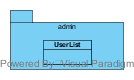
\includegraphics[scale=4, max width=\textwidth, max height=\myheight]{../img/diagrammiClassi/client/controller/admin.png}
		\caption{Diagramma package - client::controller::admin}
	\end{figure}
\end{center}\hypertarget{client::controller::admin::UsersList}{}
\subsubsubsection[UsersList]{client::controller::admin::UsersList}
\begin{figure}[H]
	\centering
	\begin{tikzpicture}
	\umlclass{client::controller::admin::UsersList} {--scope : Object\\--userService : UserService\\--roleService : RoleService\\--usersList : User[]\\--roles : Role []\\--roleFilter : String\\--myOrderBy : String}{+UsersList(scope : Object, roleService : RoleService, userService : UserService)\\+changeUserRole(user  : User) : void\\+deleteUser(user  : User) : void\\+filterByRole(roleName : String) : void\\+getUsersList() : User[]\\+getRoles() : Role []\\+getMyOrderBy() : String\\+setUsersList(usersList : User[]) : void\\+setRoles(roles : Role []) : void\\+setMyOrderBy(myOrderBy : String) : void}
	\end{tikzpicture}
	\caption{Diagramma classe - client::controller::admin::UsersList}
\end{figure}\begin{description}
\item[Descrizione] \hfill \\
Classe che si occupa della gestione di tutti gli utenti presenti nell'applicazione. In particolare gestisce l'eventuale cambio di ruolo di un utente e la sua rimozione dal sistema.
\item[Utilizzo] \hfill \\
Carica la view che permette avere la lista completa dei tutti gli utenti, consentendo di selezionare l'utente per modificarne il ruolo o per rimuoverlo dal sistema
\item[Relazioni con altre classi] \hfill \\
\vspace{-7mm}
\begin{description}
	\item[\hyperlink{client::model::data::User}{client::model::data::User}] \hfill \\
	Relazione uscente, lista di utenti
	\item[\hyperlink{client::model::data::Role}{client::model::data::Role}] \hfill \\
	Relazione uscente, lista di tutti i ruoli che può assumere un utente
	\item[\hyperlink{client::model::service::RoleService}{client::model::service::RoleService}] \hfill \\
	Relazione uscente, campo dati che rappresenta un oggetto RoleService
	\item[\hyperlink{client::model::service::UserService}{client::model::service::UserService}] \hfill \\
	Relazione uscente, campo dati che rappresenta un oggetto UserService
\end{description}

\item[Attributi] \hfill \\
\vspace{-7mm}
\begin{itemize}
	\item scope : Object $\rightarrow$ oggetto di angular che fa riferimento ad una porzione di model di pertinenza di uno specifico controller
	\item userService : UserService $\rightarrow$ campo dati che rappresenta un oggetto UserService
	\item roleService : RoleService $\rightarrow$ campo dati che rappresenta un oggetto RoleService
	\item usersList : User[] $\rightarrow$ lista di utenti
	\item roles : Role [] $\rightarrow$ lista di tutti i ruoli che può assumere un utente
	\item roleFilter : String $\rightarrow$ rappresenta il name di un ruolo da filtrare
	\item myOrderBy : String $\rightarrow$ rappresenta il campo di user da ordinare
\end{itemize}

\item[Metodi] \hfill \\
\vspace{-7mm}
\begin{itemize}
	\item UsersList(scope : Object, roleService : RoleService, userService : UserService) $\rightarrow$ costruttore della classe\begin{itemize}
		\item scope $\rightarrow$ oggetto di angular che fa riferimento ad una porzione di model di pertinenza di uno specifico controller
		\item roleService $\rightarrow$ campo dati che rappresenta un oggetto RoleService
		\item userService $\rightarrow$ campo dati che rappresenta un oggetto UserService
	\end{itemize}
	
	\item changeUserRole(user  : User) : void $\rightarrow$ cambia il ruolo di un utente dato in input\begin{itemize}
		\item user  $\rightarrow$ contiene l'utente a cui serve cambiare il ruolo
	\end{itemize}
	
	\item deleteUser(user  : User) : void $\rightarrow$ elimina l'utente passato per parametro\begin{itemize}
		\item user  $\rightarrow$ contiene l'utente da eliminare 
	\end{itemize}
	
	\item filterByRole(roleName : String) : void $\rightarrow$ filtra la lista degli utenti per ruolo\begin{itemize}
		\item roleName $\rightarrow$ name del Role
	\end{itemize}
	
	\item getUsersList() : User[] $\rightarrow$ metodo getter
	\item getRoles() : Role [] $\rightarrow$ metodo getter
	\item getMyOrderBy() : String $\rightarrow$ metodo getter
	\item setUsersList(usersList : User[]) : void $\rightarrow$ metodo setter\begin{itemize}
		\item usersList $\rightarrow$ lista di utenti
	\end{itemize}
	
	\item setRoles(roles : Role []) : void $\rightarrow$ metodo setter\begin{itemize}
		\item roles $\rightarrow$ lista di tutti i ruoli che può assumere un utente
	\end{itemize}
	
	\item setMyOrderBy(myOrderBy : String) : void $\rightarrow$ metodo setter\begin{itemize}
		\item myOrderBy $\rightarrow$ rappresenta il campo di user da ordinare
	\end{itemize}
	
\end{itemize}

\end{description}

\vspace{0.5cm}
\subsubsection{client::controller::user}
È il package che contiene tutte le classi che costituiscono i controller della porzione client per un utente generico registrato. Ogni componente si occupa della gestione di una particolare porzione dell'interfaccia di un utente generico registrato.\begin{center}
	\begin{figure}[H]
		\centering 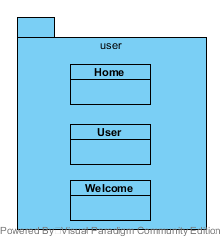
\includegraphics[scale=4, max width=\textwidth, max height=\myheight]{../img/diagrammiClassi/client/controller/user.png}
		\caption{Diagramma package - client::controller::user}
	\end{figure}
\end{center}\hypertarget{client::controller::user::Welcome}{}
\subsubsubsection[Welcome]{client::controller::user::Welcome}
\begin{figure}[H]
	\centering
	\begin{tikzpicture}
	\umlclass{client::controller::user::Welcome} {}{+Welcome()}
	\end{tikzpicture}
	\caption{Diagramma classe - client::controller::user::Welcome}
\end{figure}\begin{description}
\item[Descrizione] \hfill \\
Classe che si occupa della visualizzazione della pagina di benvenuto
\item[Metodi] \hfill \\
\vspace{-7mm}
\begin{itemize}
	\item Welcome() $\rightarrow$ costruttore della classe
\end{itemize}

\end{description}

\vspace{0.5cm}
\hypertarget{client::controller::user::Home}{}
\subsubsubsection[Home]{client::controller::user::Home}
\begin{figure}[H]
	\centering
	\begin{tikzpicture}
	\umlclass{client::controller::user::Home} {--cookies : Object\\--location : Object\\--rootScope : Object\\--sessionService : SessionService\\--scope : Object}{+logout() : void\\+Logout(scope : Object, rootScope : Object, sessionService : SessionService, cookies : Object)}
	\end{tikzpicture}
	\caption{Diagramma classe - client::controller::user::Home}
\end{figure}\begin{description}
\item[Descrizione] \hfill \\
Classe che si occupa della gestione della home page di un utente generico registrato
\item[Relazioni con altre classi] \hfill \\
\vspace{-7mm}
\begin{description}
	\item[\hyperlink{client::model::service::SessionService}{client::model::service::SessionService}] \hfill \\
	Relazione uscente, campo dati che rappresenta un oggetto SessionService
\end{description}

\item[Attributi] \hfill \\
\vspace{-7mm}
\begin{itemize}
	\item cookies : Object $\rightarrow$ oggetto di angular che permette di manipolare i cookies
	\item location : Object $\rightarrow$ oggetto di angular che analizza l'URL nella barra degli indirizzi del browser e lo rende disponibile all'applicazione
	\item rootScope : Object $\rightarrow$ oggetto di angular che identifica l’elemento con attributo ng-app
	\item sessionService : SessionService $\rightarrow$ campo dati che rappresenta un oggetto SessionService
	\item scope : Object $\rightarrow$ oggetto di angular che fa riferimento ad una porzione di model di pertinenza di uno specifico controller
\end{itemize}

\item[Metodi] \hfill \\
\vspace{-7mm}
\begin{itemize}
	\item logout() : void $\rightarrow$ esegue il logout dell'utente che è autenticato distruggendo i cookies di sessione
	\item Logout(scope : Object, rootScope : Object, sessionService : SessionService, cookies : Object) $\rightarrow$ costruttore della classe\begin{itemize}
		\item scope $\rightarrow$ oggetto di angular che fa riferimento ad una porzione di model di pertinenza di uno specifico controller
		\item rootScope $\rightarrow$ oggetto di angular che identifica l’elemento con attributo ng-app
		\item sessionService $\rightarrow$ campo dati che rappresenta un oggetto SessionService
		\item cookies $\rightarrow$ oggetto di angular che permette di manipolare i cookies
	\end{itemize}
	
\end{itemize}

\end{description}

\vspace{0.5cm}
\hypertarget{client::controller::user::User}{}
\subsubsubsection[User]{client::controller::user::User}
\begin{figure}[H]
	\centering
	\begin{tikzpicture}
	\umlclass{client::controller::user::User} {--scope : Object\\--check : Check\\--rootScope : Object\\--userService : UserService\\--errorPassword : Error\\--errorInformation : Error\\--userName : String\\--newPassword : String\\--fullName : String\\--repeatPassword : String\\--oldPassword : String\\--successInformation : boolean\\--successPassword : boolean}{+User(check : Check, rootScope : Object, scope : Object, userService : UserService)\\+checkFullName() : boolean\\+checkPassword() : boolean\\+checkUserName() : boolean\\+checkRepeatPassword() : boolean\\+submitInformation() : void\\+submitPassword() : void\\+getErrorPassword() : Error\\+getErrorInformation() : Error\\+getUserName() : String\\+getNewPassword() : String\\+getFullName() : String\\+getRepeatPassword() : String\\+getOldPassword() : String\\+getSuccessInformation() : boolean\\+getSuccessPassword() : boolean\\+setErrorPassword(errorPassword : Error) : void\\+setErrorInformation(errorInformation : Error) : void\\+setUserName(userName : String) : void\\+setNewPassword(newPassword : String) : void\\+setFullName(fullName : String) : void\\+setRepeatPassword(repeatPassword : String) : void\\+setOldPassword(oldPassword : String) : void\\+setSuccessInformation(successInformation : boolean) : void\\+setSuccessPassword(successPassword : boolean) : void}
	\end{tikzpicture}
	\caption{Diagramma classe - client::controller::user::User}
\end{figure}\begin{description}
\item[Descrizione] \hfill \\
Classe per la gestione del profilo di un'utente generico registrato
\item[Relazioni con altre classi] \hfill \\
\vspace{-7mm}
\begin{description}
	\item[\hyperlink{client::util::Check}{client::util::Check}] \hfill \\
	Relazione uscente, campo dati che rappresenta un oggetto Check
	\item[\hyperlink{client::model::service::UserService}{client::model::service::UserService}] \hfill \\
	Relazione uscente, campo dati che rappresenta un oggetto UserService
	\item[\hyperlink{client::model::data::Error}{client::model::data::Error}] \hfill \\
	Relazione uscente, oggetto che rappresenta un errore da visualizzare all'utente sulla password
	\item[\hyperlink{client::model::data::Error}{client::model::data::Error}] \hfill \\
	Relazione uscente, oggetto che rappresenta un errore da visualizzare all'utente sui dati inseriti
\end{description}

\item[Attributi] \hfill \\
\vspace{-7mm}
\begin{itemize}
	\item scope : Object $\rightarrow$ oggetto di angular che fa riferimento ad una porzione di model di pertinenza di uno specifico controller
	\item check : Check $\rightarrow$ campo dati che rappresenta un oggetto Check
	\item rootScope : Object $\rightarrow$ oggetto di angular che identifica l’elemento con attributo ng-app
	\item userService : UserService $\rightarrow$ campo dati che rappresenta un oggetto UserService
	\item errorPassword : Error $\rightarrow$ oggetto che rappresenta un errore da visualizzare all'utente sulla password
	\item errorInformation : Error $\rightarrow$ oggetto che rappresenta un errore da visualizzare all'utente sui dati inseriti
	\item userName : String $\rightarrow$ rappresenta il campo userName nella View
	\item newPassword : String $\rightarrow$ rappresenta il campo newPassword nella View	
	\item fullName : String $\rightarrow$ rappresenta il campo fullName nella View
	\item repeatPassword : String $\rightarrow$ rappresenta il campo repeatPassword nella view	
	\item oldPassword : String $\rightarrow$ rappresenta il campo oldPassword nella view
	\item successInformation : boolean $\rightarrow$ rappresenta se visualizzare il messaggio di invio con successo dei dati utente
	\item successPassword : boolean $\rightarrow$ rappresenta se visualizzare il messaggio di invio con successo dei dati password utente
\end{itemize}

\item[Metodi] \hfill \\
\vspace{-7mm}
\begin{itemize}
	\item User(check : Check, rootScope : Object, scope : Object, userService : UserService) $\rightarrow$ costruttore della classe\begin{itemize}
		\item check $\rightarrow$ campo dati che rappresenta un oggetto Check
		\item rootScope $\rightarrow$ oggetto di angular che identifica l’elemento con attributo ng-app
		\item scope $\rightarrow$ oggetto di angular che fa riferimento ad una porzione di model di pertinenza di uno specifico controller
		\item userService $\rightarrow$ campo dati che rappresenta un oggetto UserService
	\end{itemize}
	
	\item checkFullName() : boolean $\rightarrow$ controlla se il nome inserito ha i requisiti minimi richiamando il relativo metodo nella classe Check
	\item checkPassword() : boolean $\rightarrow$ controlla se la password inserita ha i requisiti minimi richiamando il relativo metodo nella classe Check
	\item checkUserName() : boolean $\rightarrow$ controlla se lo username abbia i requisiti minimi richiamando il relativo metodo nella classe Check
	\item checkRepeatPassword() : boolean $\rightarrow$ controlla se la password sia uguale a quella inserita nel campo "Ripeti password"
	\item submitInformation() : void $\rightarrow$ invia i dati dell'utente al servizio che ne effettua l'aggiornamento
	\item submitPassword() : void $\rightarrow$ invia i dati sulla password dell'utente modificata al servizio che ne effettua l'aggiornamento
	\item getErrorPassword() : Error $\rightarrow$ metodo getter
	\item getErrorInformation() : Error $\rightarrow$ metodo getter
	\item getUserName() : String $\rightarrow$ metodo getter
	\item getNewPassword() : String $\rightarrow$ metodo getter
	\item getFullName() : String $\rightarrow$ metodo getter
	\item getRepeatPassword() : String $\rightarrow$ metodo getter
	\item getOldPassword() : String $\rightarrow$ metodo getter
	\item getSuccessInformation() : boolean $\rightarrow$ metodo getter
	\item getSuccessPassword() : boolean $\rightarrow$ metodo getter
	\item setErrorPassword(errorPassword : Error) : void $\rightarrow$ metodo setter\begin{itemize}
		\item errorPassword $\rightarrow$ oggetto che rappresenta un errore da visualizzare all'utente sulla password
	\end{itemize}
	
	\item setErrorInformation(errorInformation : Error) : void $\rightarrow$ metodo setter\begin{itemize}
		\item errorInformation $\rightarrow$ oggetto che rappresenta un errore da visualizzare all'utente sui dati inseriti
	\end{itemize}
	
	\item setUserName(userName : String) : void $\rightarrow$ metodo setter\begin{itemize}
		\item userName $\rightarrow$ rappresenta il campo userName nella View
	\end{itemize}
	
	\item setNewPassword(newPassword : String) : void $\rightarrow$ metodo setter\begin{itemize}
		\item newPassword $\rightarrow$ rappresenta il campo newPassword nella View	
	\end{itemize}
	
	\item setFullName(fullName : String) : void $\rightarrow$ metodo setter\begin{itemize}
		\item fullName $\rightarrow$ rappresenta il campo fullName nella View
	\end{itemize}
	
	\item setRepeatPassword(repeatPassword : String) : void $\rightarrow$ metodo setter\begin{itemize}
		\item repeatPassword $\rightarrow$ rappresenta il campo repeatPassword nella view	
	\end{itemize}
	
	\item setOldPassword(oldPassword : String) : void $\rightarrow$ metodo setter\begin{itemize}
		\item oldPassword $\rightarrow$ rappresenta il campo oldPassword nella view
	\end{itemize}
	
	\item setSuccessInformation(successInformation : boolean) : void $\rightarrow$ metodo setter\begin{itemize}
		\item successInformation $\rightarrow$ rappresenta se visualizzare il messaggio di invio con successo dei dati utente
	\end{itemize}
	
	\item setSuccessPassword(successPassword : boolean) : void $\rightarrow$ metodo setter\begin{itemize}
		\item successPassword $\rightarrow$ rappresenta se visualizzare il messaggio di invio con successo dei dati password utente
	\end{itemize}
	
\end{itemize}

\end{description}

\vspace{0.5cm}
\subsection{client::util}
Il package che contiene le classi di utilità del client.\begin{center}
	\begin{figure}[H]
		\centering 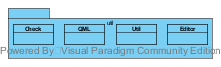
\includegraphics[scale=4, max width=\textwidth, max height=\myheight]{../img/diagrammiClassi/client/util.png}
		\caption{Diagramma package - client::util}
	\end{figure}
\end{center}\hypertarget{client::util::Check}{}
\subsubsection[Check]{client::util::Check}
\begin{figure}[H]
	\centering
	\begin{tikzpicture}
	\umlclass{client::util::Check} {}{+checkPassword(password : String) : boolean\\+checkUserName(userName : String) : boolean\\+checkTitle(title : String) : boolean\\+Check()}
	\end{tikzpicture}
	\caption{Diagramma classe - client::util::Check}
\end{figure}\begin{description}
\item[Descrizione] \hfill \\
Classe che controlla se la password,  l'userName o titolo rispettino il formato scelto
\item[Relazioni con altre classi] \hfill \\
\vspace{-7mm}
\begin{description}
	\item[\hyperlink{client::controller::public::LogIn}{client::controller::public::LogIn}] \hfill \\
	Relazione entrante, campo dati che rappresenta un oggetto Check
	\item[\hyperlink{client::controller::public::SignUp}{client::controller::public::SignUp}] \hfill \\
	Relazione entrante, campo dati che rappresenta un oggetto Check
	\item[\hyperlink{client::controller::user::User}{client::controller::user::User}] \hfill \\
	Relazione entrante, campo dati che rappresenta un oggetto Check
\end{description}

\item[Metodi] \hfill \\
\vspace{-7mm}
\begin{itemize}
	\item checkPassword(password : String) : boolean $\rightarrow$ metodo che controlla la conformità della password rispetto ai parametri scelti: che sia maggiore o uguale a 6 caratteri\begin{itemize}
		\item password $\rightarrow$ contiene la password da controllare  
	\end{itemize}
	
	\item checkUserName(userName : String) : boolean $\rightarrow$ metodo che controlla la conformità dell'username rispetto ai parametri scelti: che sia maggiore o uguale a 6 caratteri\begin{itemize}
		\item userName $\rightarrow$ contiene il username da controllare 
	\end{itemize}
	
	\item checkTitle(title : String) : boolean $\rightarrow$ metodo che controlla la conformità del titolo rispetto ai parametri scelti: che non sia vuoto\begin{itemize}
		\item title $\rightarrow$ contiene il titolo da controllare 
	\end{itemize}
	
	\item Check() $\rightarrow$ costruttore della classe
\end{itemize}

\end{description}

\vspace{0.5cm}
\hypertarget{client::util::Util}{}
\subsubsection[Util]{client::util::Util}
\begin{figure}[H]
	\centering
	\begin{tikzpicture}
	\umlclass{client::util::Util} {}{+alert(message : String) : void\\+confirm(message : String) : boolean\\+Util()}
	\end{tikzpicture}
	\caption{Diagramma classe - client::util::Util}
\end{figure}\begin{description}
\item[Descrizione] \hfill \\
Classe che espone metodi pubblici utili a varie classi del sistema
\item[Relazioni con altre classi] \hfill \\
\vspace{-7mm}
\begin{description}
	\item[\hyperlink{client::controller::teacher::ManageQuestions}{client::controller::teacher::ManageQuestions}] \hfill \\
	Relazione entrante, campo dati che rappresenta un oggetto Util
	\item[\hyperlink{client::controller::teacher::ManageQuestionnaires}{client::controller::teacher::ManageQuestionnaires}] \hfill \\
	Relazione entrante, campo dati che rappresenta un oggetto Util
	\item[\hyperlink{client::controller::teacher::ManageTags}{client::controller::teacher::ManageTags}] \hfill \\
	Relazione entrante, campo dati che rappresenta un oggetto Util
	\item[\hyperlink{client::controller::student::ExecuteQuestionnaire}{client::controller::student::ExecuteQuestionnaire}] \hfill \\
	Relazione entrante, campo dati che rappresenta un oggetto Util
\end{description}

\item[Metodi] \hfill \\
\vspace{-7mm}
\begin{itemize}
	\item alert(message : String) : void $\rightarrow$ stampa un pop-up con un messaggio\begin{itemize}
		\item message $\rightarrow$ 
	\end{itemize}
	
	\item confirm(message : String) : boolean $\rightarrow$ stampa un messaggio chiedendo all'utente di confermare un'azione\begin{itemize}
		\item message $\rightarrow$ 
	\end{itemize}
	
	\item Util() $\rightarrow$ costruttore della classe
\end{itemize}

\end{description}

\vspace{0.5cm}
\hypertarget{client::util::QML}{}
\subsubsection[QML]{client::util::QML}
\begin{figure}[H]
	\centering
	\begin{tikzpicture}
	\umlclass{client::util::QML} {}{+parse(plainText : String) : Json\\+preview(plainText : String) : void\\+QML()}
	\end{tikzpicture}
	\caption{Diagramma classe - client::util::QML}
\end{figure}\begin{description}
\item[Descrizione] \hfill \\
Classe che provvede metodi per gestire il QML
\item[Relazioni con altre classi] \hfill \\
\vspace{-7mm}
\begin{description}
	\item[\hyperlink{client::controller::teacher::ManageQuestionnaires}{client::controller::teacher::ManageQuestionnaires}] \hfill \\
	Relazione entrante, campo dati che rappresenta un oggetto QML
	\item[\hyperlink{client::controller::teacher::ManageQuestions}{client::controller::teacher::ManageQuestions}] \hfill \\
	Relazione entrante, campo dati che rappresenta un oggetto QML
	\item[\hyperlink{client::controller::teacher::ManipulateQuestion}{client::controller::teacher::ManipulateQuestion}] \hfill \\
	Relazione entrante, campo dati che rappresenta un oggetto QML
	\item[\hyperlink{client::controller::teacher::ManipulateQuestionnaire}{client::controller::teacher::ManipulateQuestionnaire}] \hfill \\
	Relazione entrante, campo dati che rappresenta un oggetto QML
\end{description}

\item[Metodi] \hfill \\
\vspace{-7mm}
\begin{itemize}
	\item parse(plainText : String) : Json $\rightarrow$ provvede a fare il parsing del QML e restituisce un oggetto Json con i seguenti campi: status è un booleano che rappresenta la validità del QML, type è una stringa che rappresenta il tipo di domanda, body è una stringa che contiene il codice HTML per renderizzare la domanda, answers è un array di possibili risposte, answer rappresenta la risposta esatta.\begin{itemize}
		\item plainText $\rightarrow$ 
	\end{itemize}
	
	\item preview(plainText : String) : void $\rightarrow$ provvede a fornire un'anteprima di una domanda da QML in HTML\begin{itemize}
		\item plainText $\rightarrow$ 
	\end{itemize}
	
	\item QML() $\rightarrow$ costruttore della classe
\end{itemize}

\end{description}

\vspace{0.5cm}
\hypertarget{client::util::Editor}{}
\subsubsection[Editor]{client::util::Editor}
\begin{figure}[H]
	\centering
	\begin{tikzpicture}
	\umlclass{client::util::Editor} {}{+editor() : SimpleMDE\\+Editor()}
	\end{tikzpicture}
	\caption{Diagramma classe - client::util::Editor}
\end{figure}\begin{description}
\item[Descrizione] \hfill \\
Classe che si occupa di gestire l'editor per il QML
\item[Relazioni con altre classi] \hfill \\
\vspace{-7mm}
\begin{description}
	\item[\hyperlink{client::controller::teacher::ManipulateQuestion}{client::controller::teacher::ManipulateQuestion}] \hfill \\
	Relazione entrante, campo dati che rappresenta un oggetto Editor
\end{description}

\item[Metodi] \hfill \\
\vspace{-7mm}
\begin{itemize}
	\item editor() : SimpleMDE $\rightarrow$ provvede a creare un editor per il QML
	\item Editor() $\rightarrow$ costruttore della classe
\end{itemize}

\end{description}

\vspace{0.5cm}
\subsection{client::app}
Questo Package ha il compito di fornire la configurazione e avviare il client.\begin{center}
	\begin{figure}[H]
		\centering 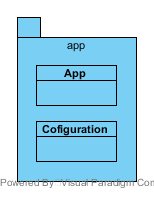
\includegraphics[scale=4, max width=\textwidth, max height=\myheight]{../img/diagrammiClassi/client/app.png}
		\caption{Diagramma package - client::app}
	\end{figure}
\end{center}\hypertarget{client::app::App}{}
\subsubsection[App]{client::app::App}
\begin{figure}[H]
	\centering
	\begin{tikzpicture}
	\umlclass{client::app::App} {}{+App()}
	\end{tikzpicture}
	\caption{Diagramma classe - client::app::App}
\end{figure}\begin{description}
\item[Descrizione] \hfill \\
Classe che si occupa di avviare il client e attivare i moduli angularjs
\item[Metodi] \hfill \\
\vspace{-7mm}
\begin{itemize}
	\item App() $\rightarrow$ costruttore della classe
\end{itemize}

\end{description}

\vspace{0.5cm}
\hypertarget{client::app::Configuration}{}
\subsubsection[Configuration]{client::app::Configuration}
\begin{figure}[H]
	\centering
	\begin{tikzpicture}
	\umlclass{client::app::Configuration} {--remote : String}{+Configuration(remote : String)}
	\end{tikzpicture}
	\caption{Diagramma classe - client::app::Configuration}
\end{figure}\begin{description}
\item[Descrizione] \hfill \\
Classe che rappresenta i parametri di configurazione del client
\item[Relazioni con altre classi] \hfill \\
\vspace{-7mm}
\begin{description}
	\item[\hyperlink{client::model::service::SessionService}{client::model::service::SessionService}] \hfill \\
	Relazione entrante, campo dati che rappresenta un oggetto Configuration
	\item[\hyperlink{client::model::service::UserService}{client::model::service::UserService}] \hfill \\
	Relazione entrante, campo dati che rappresenta un oggetto Configuration
	\item[\hyperlink{client::model::service::TagService}{client::model::service::TagService}] \hfill \\
	Relazione entrante, campo dati che rappresenta un oggetto Configuration
	\item[\hyperlink{client::model::service::QuestionnaireService}{client::model::service::QuestionnaireService}] \hfill \\
	Relazione entrante, campo dati che rappresenta un oggetto Configuration
	\item[\hyperlink{client::model::service::QuestionService}{client::model::service::QuestionService}] \hfill \\
	Relazione entrante, campo dati che rappresenta un oggetto Configuration
	\item[\hyperlink{client::model::service::RoleService}{client::model::service::RoleService}] \hfill \\
	Relazione entrante, campo dati che rappresenta un oggetto Configuration
\end{description}

\item[Attributi] \hfill \\
\vspace{-7mm}
\begin{itemize}
	\item remote : String $\rightarrow$ rappresenta l'indirizzo verso cui il client effettua le richieste REST
\end{itemize}

\item[Metodi] \hfill \\
\vspace{-7mm}
\begin{itemize}
	\item Configuration(remote : String) $\rightarrow$ costruttore della classe\begin{itemize}
		\item remote $\rightarrow$ rappresenta l'indirizzo verso cui il client effettua le richieste REST
	\end{itemize}
	
\end{itemize}

\end{description}


\newpage
\section{Design pattern}
Un \mgls{design pattern} descrive problemi che si presentano frequentemente nell'ambiente informatico, specificando relative soluzioni. La conoscenza dei \mgls{design pattern} facilita l’attività di progettazione, favorendo la riusabilità del codice e portando molteplici benefici in termini di manutenibilità. Possiamo suddividere i \mgls{design pattern} in quattro categorie:

\begin{itemize}
	\item \textbf{Design pattern architetturali:} che esprimono schemi di base per impostare l’organizzazione strutturale di un sistema software
	\item \textbf{Design pattern creazionali:} che forniscono un’astrazione del processo di istanziazione degli oggetti;
	\item \textbf{Design pattern strutturali:} che si occupano delle modalità di composizione di classi e oggetti per formare strutture complesse
	\item \textbf{Design pattern comportamentali:} che si occupano di algoritmi e dell’assegnamento di responsabilità tra oggetti collaboranti
\end{itemize}

\subsection{Design pattern architetturali}
\subsubsection{MVC}
\paragraph{Scopo}
Questo pattern è utilizzato per separare le responsabilità dell’applicazione a diversi componenti e permettere di fare una chiara divisione presentazione, struttura dei dati e operazioni su di essi.

\paragraph{Utilizzo}
Nel front-end viene utilizzato questo \mgls{design pattern} per dividere la presentazione dei dati dalla logica dell'applicazione e la logica di business. I vari componenti sono identificati nelle seguenti classi:

\begin{itemize}
	\item il package \texttt{client::model} è la business logic che gestisce i dati;
	\item il package \texttt{client::view} è la presentation logic che costruisce le pagine da visualizzare;
	\item il package \texttt{client::controller} è l'application logic.
\end{itemize}

\subsubsection{Middleware}
\paragraph{Scopo}
Si è scelto di utilizzare questo \mgls{design pattern} per fornire un intermediario tra i vari componenti software dell’applicazione in modo da semplificare notevolmente la loro connessione e collaborazione. Questo pattern in generale è molto utile nello sviluppo e nella gestione di sistemi distribuiti complessi, e nel nostro caso si adatta bene alla gestione di richieste \mgls{rest}.
\paragraph{Utilizzo}
Viene utilizzato dal framework \mgls{express} per fornire una libreria di funzioni comuni. Definisce una serie di livelli (o funzioni) per gestire le varie richieste dell’applicazione e richiamare i rispettivi handler. Tutti i componenti del middleware sono collegati l’uno con l’altro e ricevono a turno una richiesta in ingresso, finché uno di questi non decide di partire con l’elaborazione per poi chiamare la funzione \texttt{next}. Come si può notare è molto legato a Chain of Responsibility, che verrà descritto in seguito. Nella progettazione architetturale è utilizzato nel package \texttt{server::middleware}.

\subsection{Design pattern creazionali}

\subsubsection{Singleton}
\paragraph{Scopo}
Viene utilizzato per le classi che devono avere un’unica istanza, accessibile globalmente, durante l’esecuzione dell’applicazione.
\paragraph{Utilizzo}
Ogni modulo di \mgls{node.js} è nativamente un singleton, perché viene caricato alla prima chiamata \texttt{require} e poi tutti gli utilizzi successivi riferiscono sempre alla stessa istanza del modulo.

\subsection{Design pattern strutturali}

\subsubsection{Facade}
\paragraph{Scopo}
Viene utilizzato per rendere visibili solamente alcune componenti agli altri moduli ed avere un unico punto di accesso semplificato a un sottosistema fornendo un’interfaccia di alto livello e minimizzando dunque le comunicazioni e le dipendenze.

\paragraph{Utilizzo}
Viene utilizzato all’interno della classe \texttt{server::middleware::Loader}, la quale utilizza Facade per nascondere l’esistenza di tutti i middleware all'esterno. In questo modo le richieste vengono delegate agli oggetti appropriati senza che la classe cliente conosca le classi del sottosistema. Sarà il Facade che si occuperà di trasferire la comunicazione all’oggetto appropriato.

\subsection{Design Pattern comportamentali}
\subsubsection{Chain of Responsibility}

\paragraph{Scopo}
Viene utilizzato per far sì che un oggetto a cui viene effettuata una richiesta possa completare le richieste di più oggetti. In questo modo si evita l’accoppiamento fra il mittente di una richiesta e il destinatario. Tutti gli oggetti destinatari della richiesta sono concatenati tra di loro. Ogni nodo della catena se può esaudire la richiesta la effettua, altrimenti delega l’onere al nodo successivo. La catena viene attraversata finché un nodo non può eseguire l’ordine del mittente.

\paragraph{Utilizzo}
\mgls{express} usa chain of responsibility per la gestione dei middleware e del routing. Come già accennato è particolarmente legato al pattern Middleware. Viene utilizzato nella nostra architettura all’interno del package \texttt{server::middleware}. La classe \texttt{server::middleware::Router} gestisce la richiesta scorrendo tutta la lista delle sottoclassi e richiamando il metodo \texttt{next} finché una di queste non può soddisfarla. Nel gergo del framework Express i middleware corrispondono agli oggetti ConcreteHandler del design pattern. Sebbene il comportamento e lo scopo sia quasi identico, l’implementazione di Express presenta alcune differenze:

\begin{itemize}
	\item I middleware di Express possono essere classi con un metodo \texttt{handle} o semplici funzioni, in pieno accordo con lo stile funzionale utilizzato dalla grande maggioranza delle librerie e delle applicazioni scritte in \mgls{node.js}. Nel progetto sarà utilizzata principalmente la seconda versione.
	\item Il \mgls{design pattern} prevede che l’oggetto \texttt{Handler} abbia un riferimento \texttt{successor} all’\texttt{Handler} successivo. \mgls{express} invece passa al metodo di esecuzione del middleware una callback. Il middleware, eseguendo la callback, passa nuovamente il controllo all’oggetto del server di \mgls{express} il quale passerà il controllo al successivo middleware.
	\item \mgls{express} divide i middleware in due gruppi: i middleware standard e i middleware di gestione degli errori, si distinguono per il numero di parametri che possono gestire (3 e 4, rispettivamente). Ogni middleware può decidere se passare il controllo al prossimo middleware standard o se passare il controllo al prossimo middleware di gestione degli errori (passandogli anche l’errore da gestire). Questa funzionalità serve per permettere la gestione di errori senza utilizzare i costrutti \texttt{try-catch}, tipici dei linguaggi imperativi ma inefficaci quando si utilizza lo stile di programmazione asincrono.
	\item Ogni middleware di \mgls{express} deve essere invocato con i seguenti parametri: l’eventuale errore da gestire (se è un middleware di gestione degli errori), l’oggetto della richiesta, l’oggetto della risposta, la callback da utilizzare per passare il controllo al successivo middleware. L’ordine è rilevante.
\end{itemize}

\newpage

\section{Diagrammi di sequenza}
Qui riportati alcuni diagrammi di sequenza per facilitare la comprensione della catena delle chiamate durante il lavoro in fase di codifica.

\subsection{Server}
Vengono di seguito presentati i diagrammi di sequenza di alcune delle operazioni più significative lato \mgls{server}.

\subsubsection{Login}
Di seguito viene presentato il diagramma di sequenza per l'accesso da parte di un ospite. Gli oggetti e attori attivi durante questa interazione sono:

\begin{itemize}
	\item \textbf{router:} è l'oggetto che si occupa di smistare la richiesta in base all’URI ricevuto e ad invocare l’opportuno servizio. Tutte le richieste che arrivano al server passano per questo oggetto, il quale le instrada correttamente secondo il \mgls{design pattern} Chain of Responsibility
	\item \textbf{sessionService:} è l'oggetto che si occupa di controllare che le credenziali di accesso siano corrette e di eseguire l'accesso da parte dell'utente creando la sessione corrispondente
	\item \textbf{errorHandler:} è il \mgls{middleware} che viene invocato verso la fine della richiesta che si occupa di trasformare eventuali errori nel formato \mgls{json} richiesto Viene invocato nel caso in cui le credenziali di accesso non siano corrette
\end{itemize}

\begin{center}
	\begin{figure}[H]
		\centering 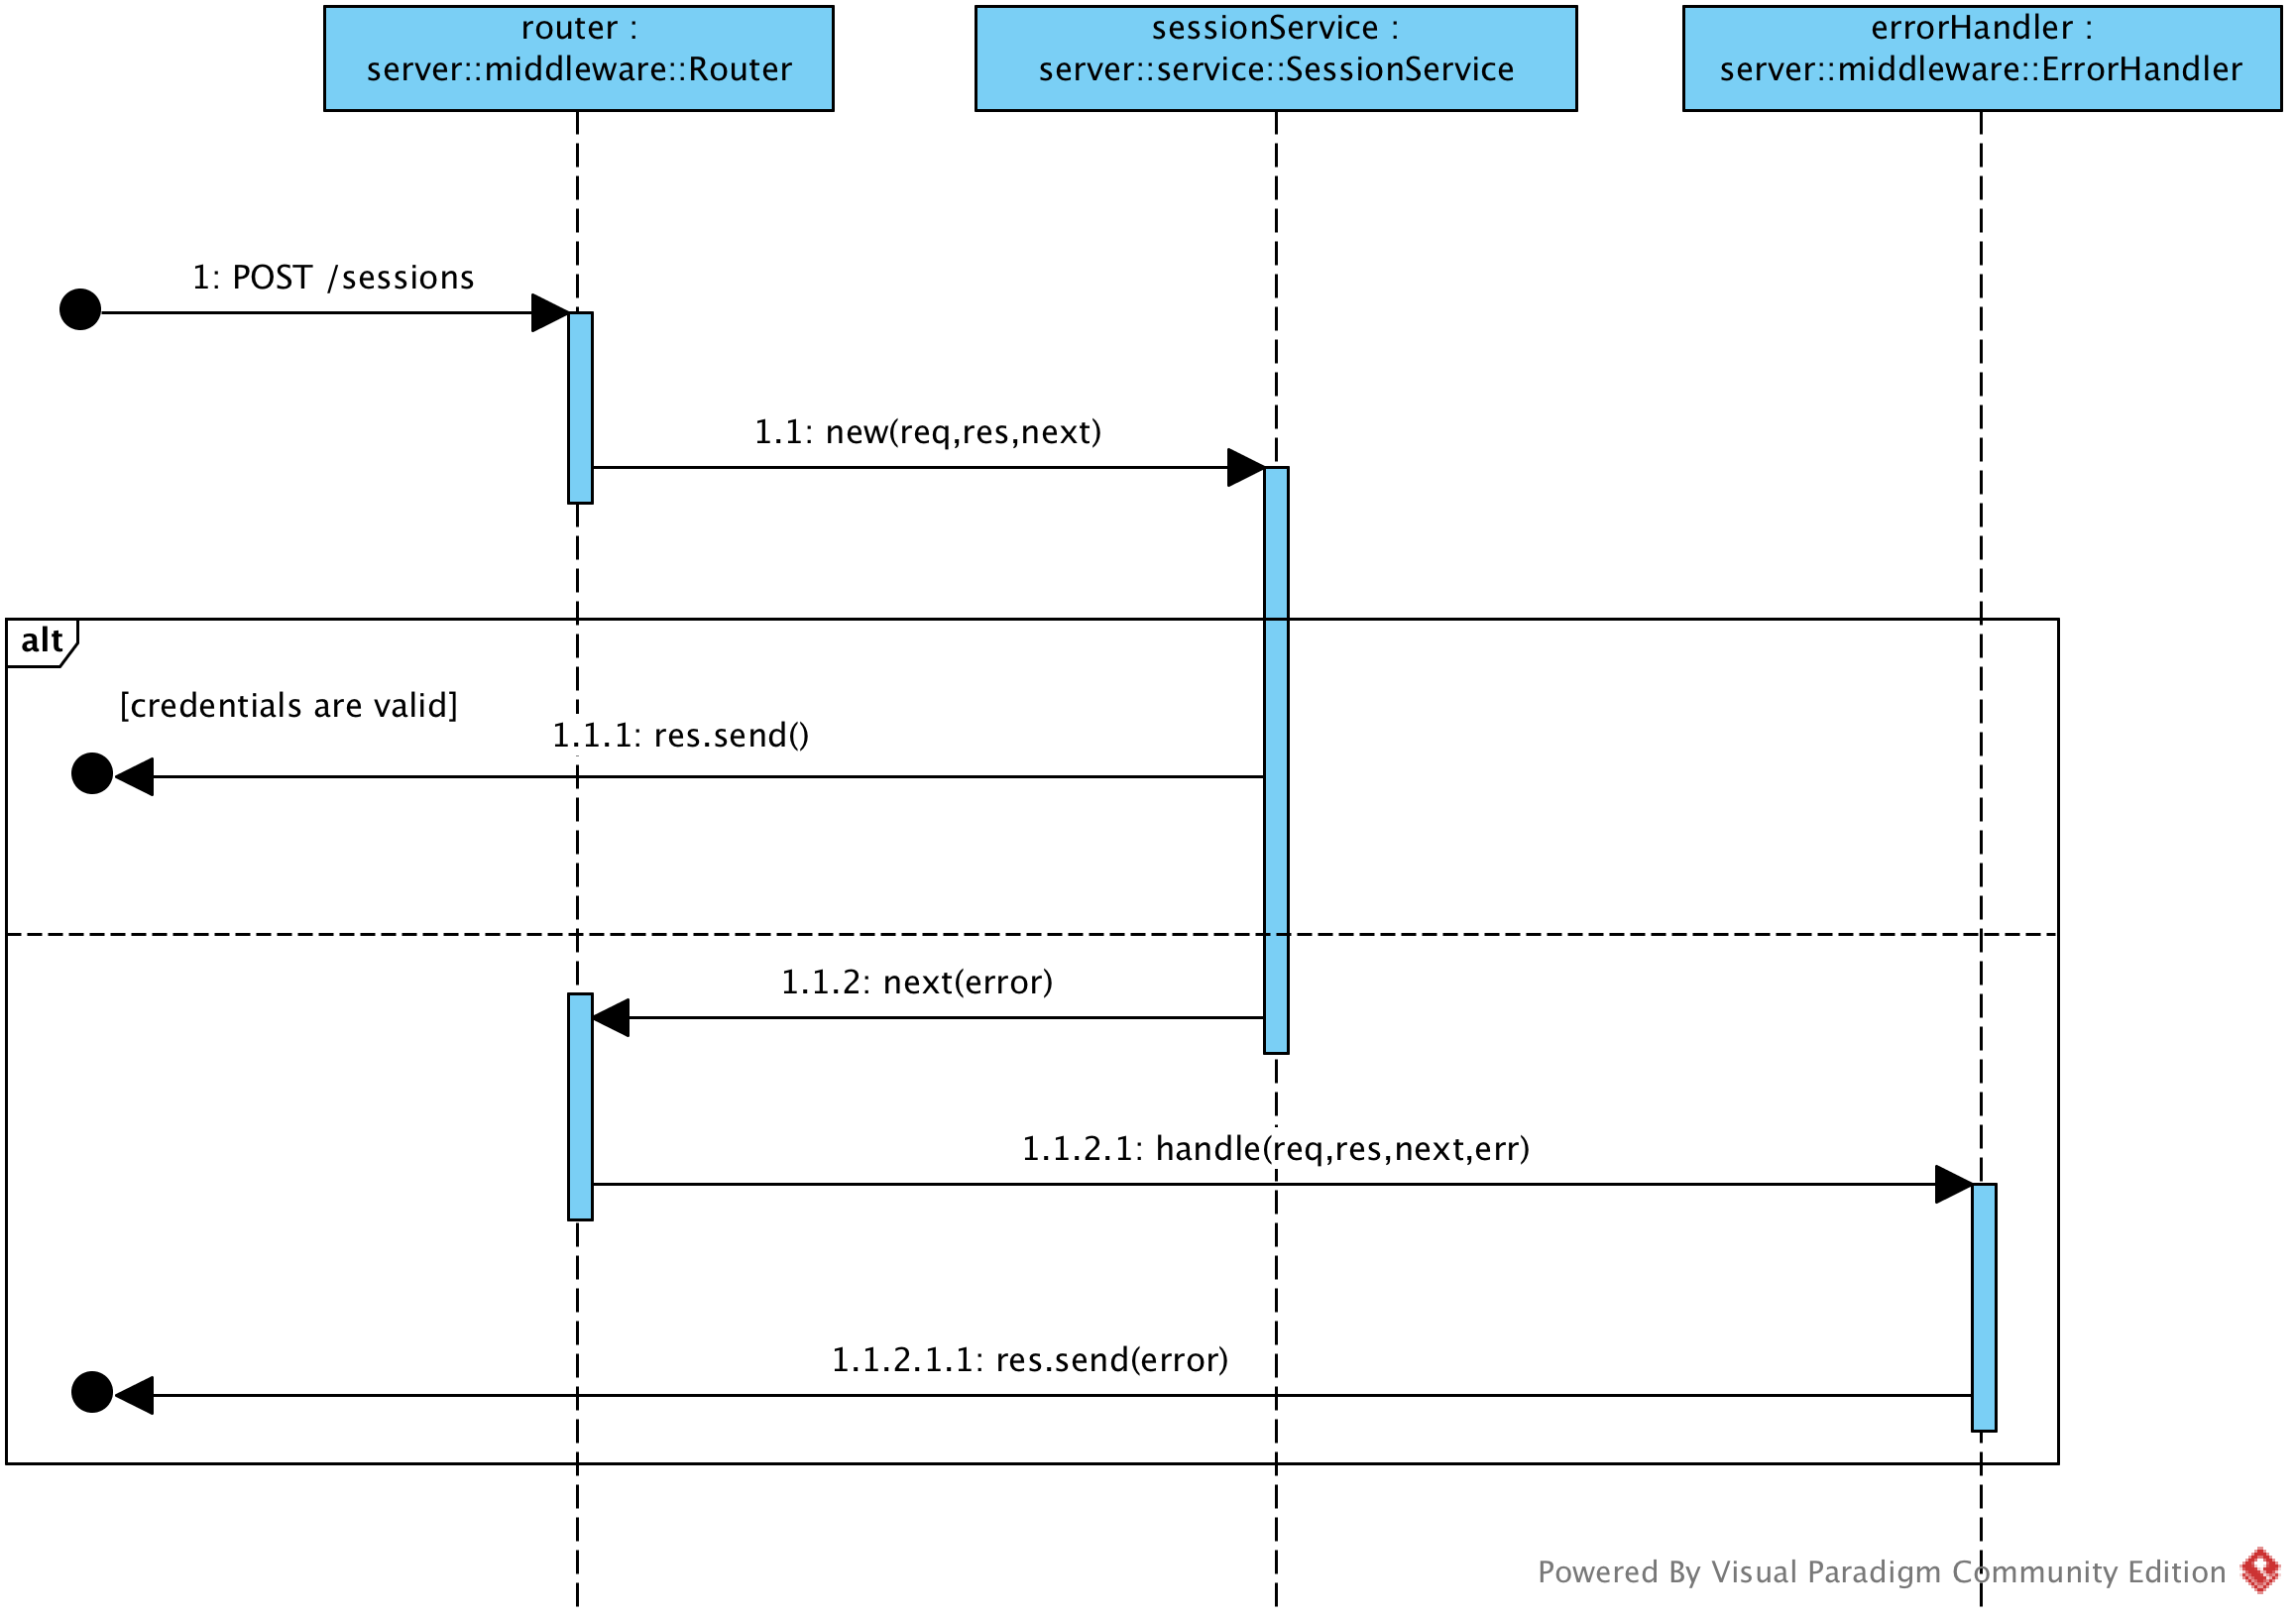
\includegraphics[max width=\myheight, angle=90]{../img/diagrammiSequenza/loginServer.png}
		\caption{Diagramma sequenza - Login Server}
	\end{figure}
\end{center}

\newpage
\subsubsection{Registrazione}
Di seguito viene presentato il diagramma di sequenza del flusso per la registrazione di un utente presso il sistema. Gli oggetti e attori attivi durante questa interazione sono:

\begin{itemize}
	\item \textbf{router:} è l'oggetto che si occupa di smistare la richiesta in base all’URI ricevuto e ad invocare l’opportuno servizio	
	\item \textbf{userService:}  è l'oggetto che si occupa di aggiungere le informazioni di un nuovo utente nel database del sistema
	\item \textbf{userCheck:} è l'oggetto che si occupa di controllare che le informazioni inserite dal nuovo utente siano corrette
	\item \textbf{errorHandler:} è il \mgls{middleware} che viene invocato verso la fine della richiesta che si occupa di trasformare eventuali errori nel formato \mgls{json} richiesto Viene invocato nel caso in cui la richiesta non sia corretta, per esempio password troppo corta o username troppo corto
\end{itemize}

\begin{center}
	\begin{figure}[H]
		\centering 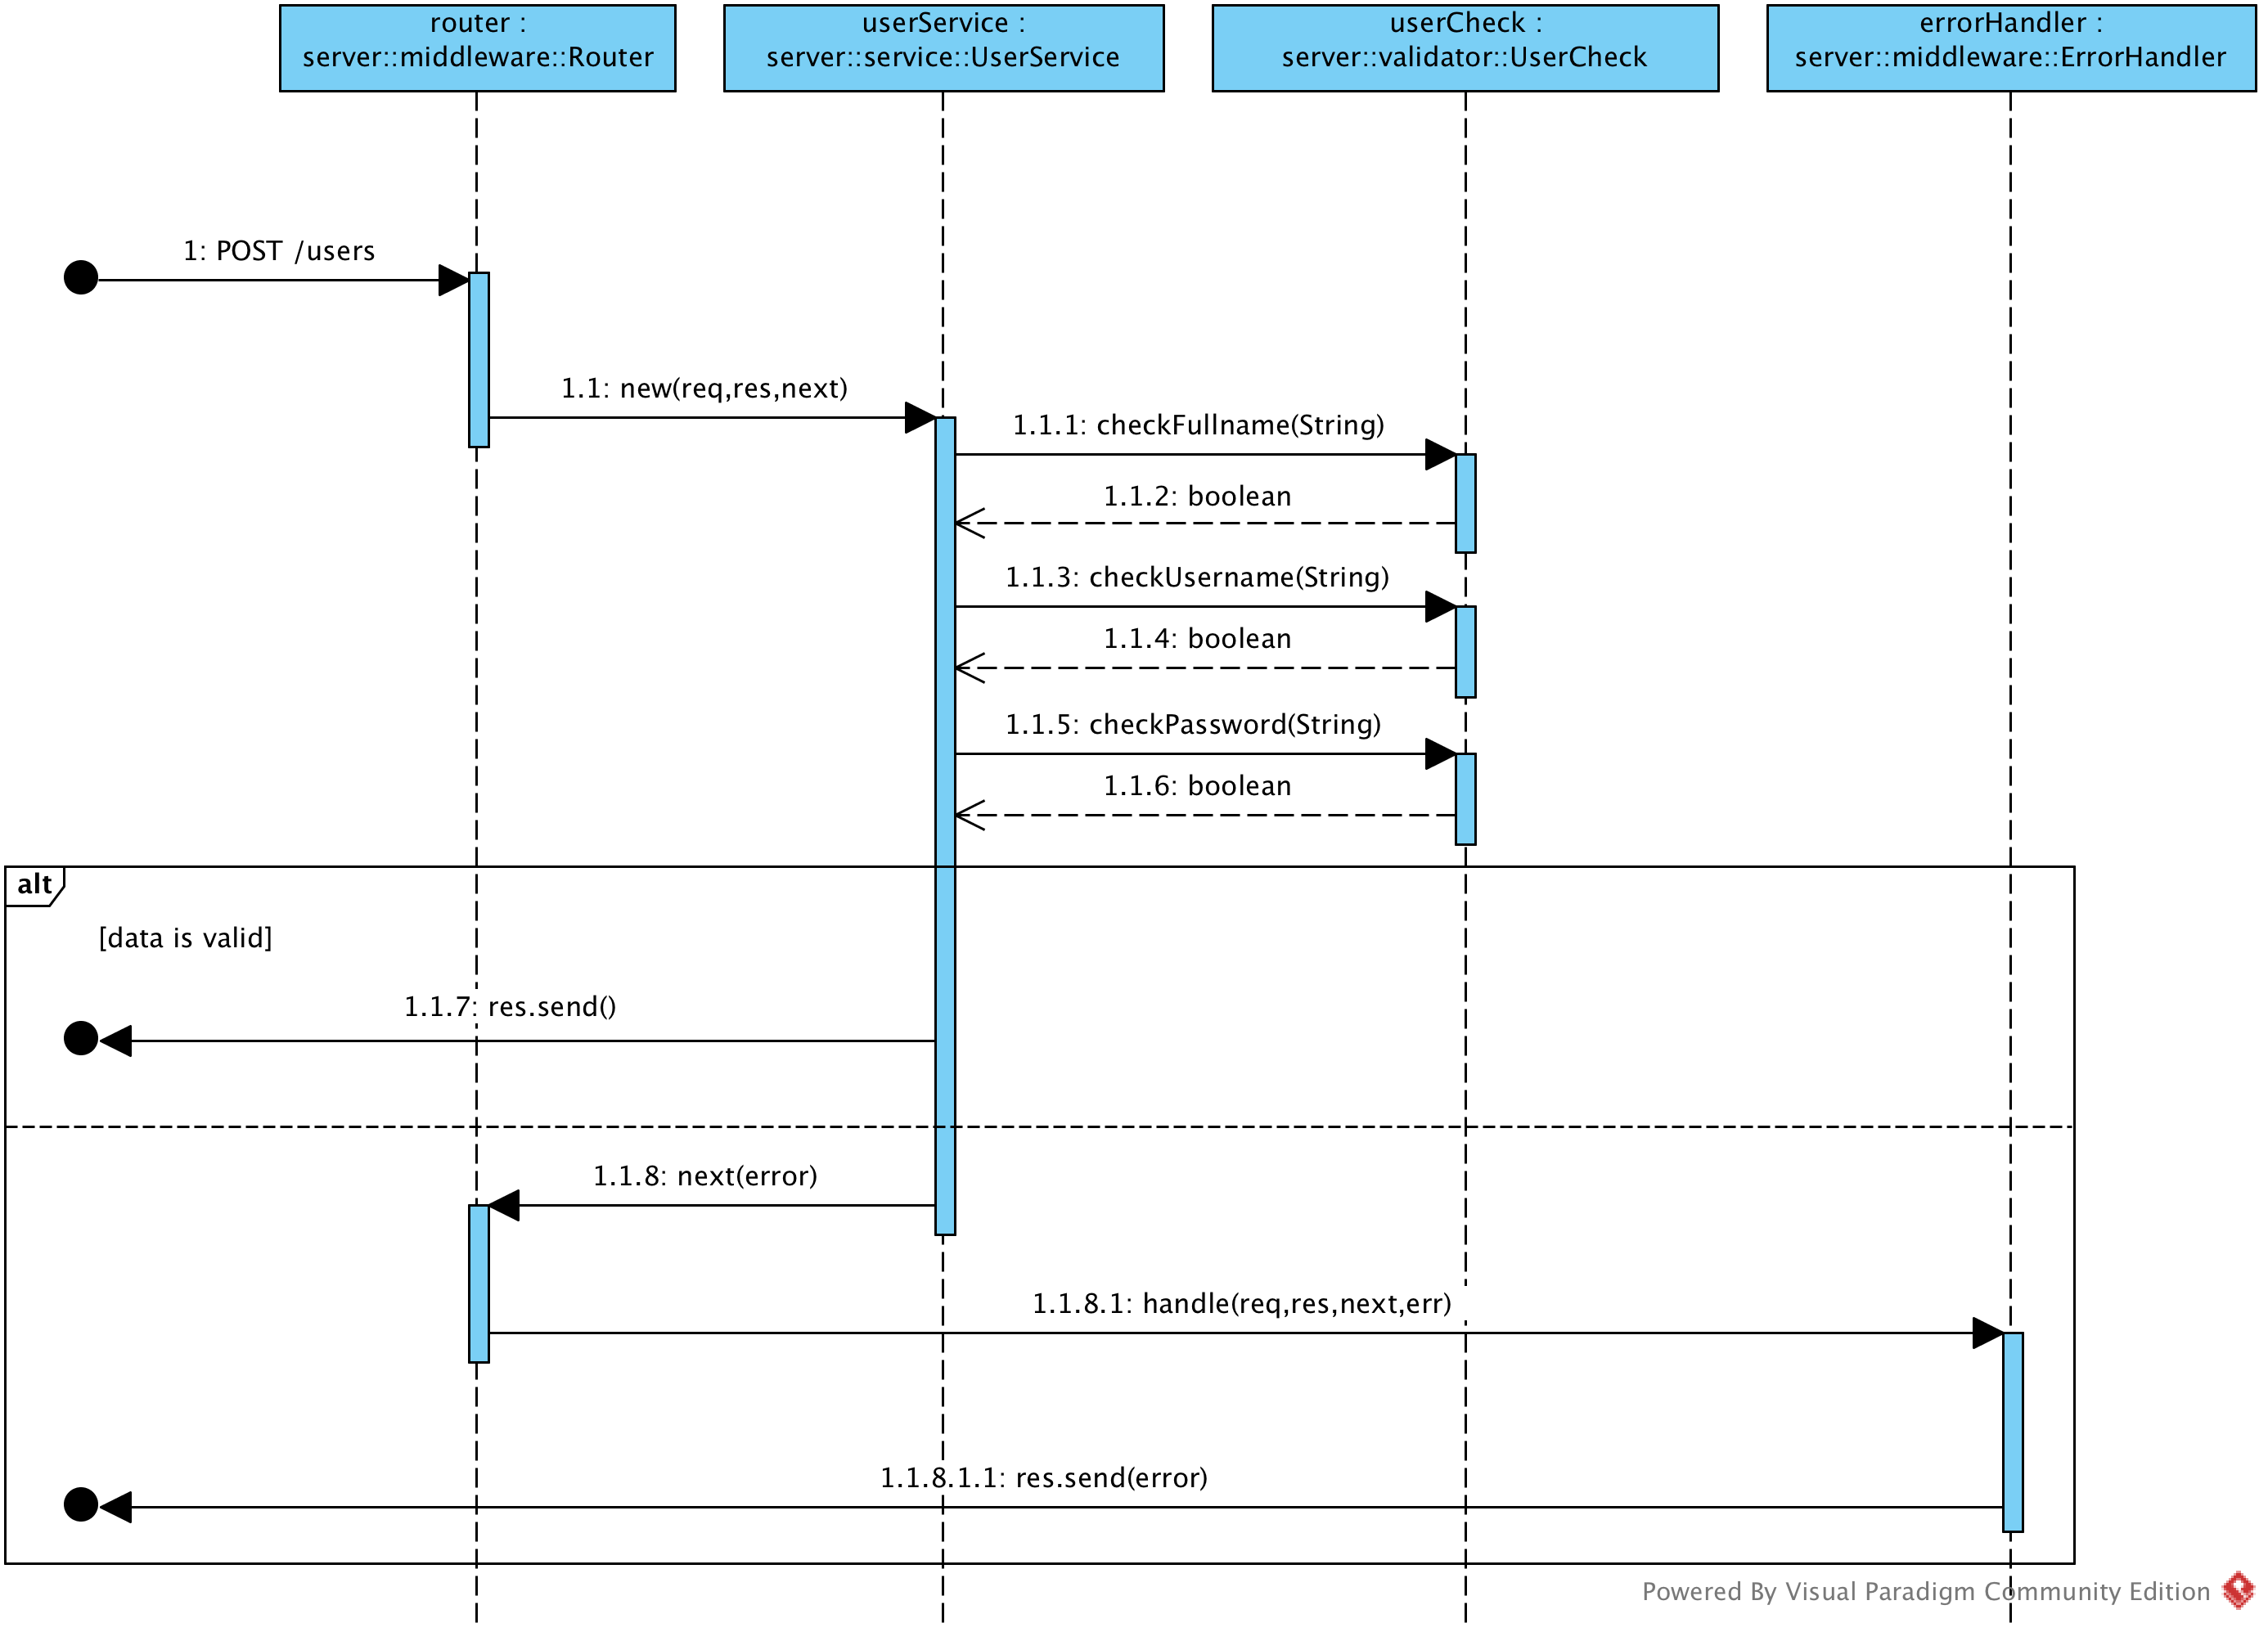
\includegraphics[max width=\myheight, angle=90]{../img/diagrammiSequenza/registrazioneServer.png}
		\caption{Diagramma sequenza - Registrazione Server}
	\end{figure}
\end{center}

\newpage
\subsubsection{Inserisci Domanda}
Di seguito viene presentato il diagramma di sequenza per l'inserimento di una domanda da parte di un docente, o utente di grado superiore. Gli oggetti e attori attivi durante questa interazione sono:

\begin{itemize}
	\item \textbf{router:} è l'oggetto che si occupa di smistare la richiesta in base all’URI ricevuto e ad invocare l’opportuno servizio
	\item \textbf{authorization:} è l'oggetto che si occupa di verificare i permessi dell'utente per ogni richiesta, in questo caso bisogna che l'utente sia almeno un docente
	\item \textbf{questionService:} è l'oggetto che si occupa di effettuare le modifiche nel database per l'aggiunta della domanda
	\item \textbf{questionCheck:} è l'oggetto che si occupa di controllare che gli attributi di una domanda siano consistenti
	\item \textbf{errorHandler:} è il \mgls{middleware} che viene invocato verso la fine della richiesta che si occupa di trasformare eventuali errori nel formato \mgls{json} richiesto. Viene invocato nel caso in cui la richiesta non sia corretta, per esempio il QML non valido
\end{itemize}

\begin{center}
	\begin{figure}[H]
		\centering 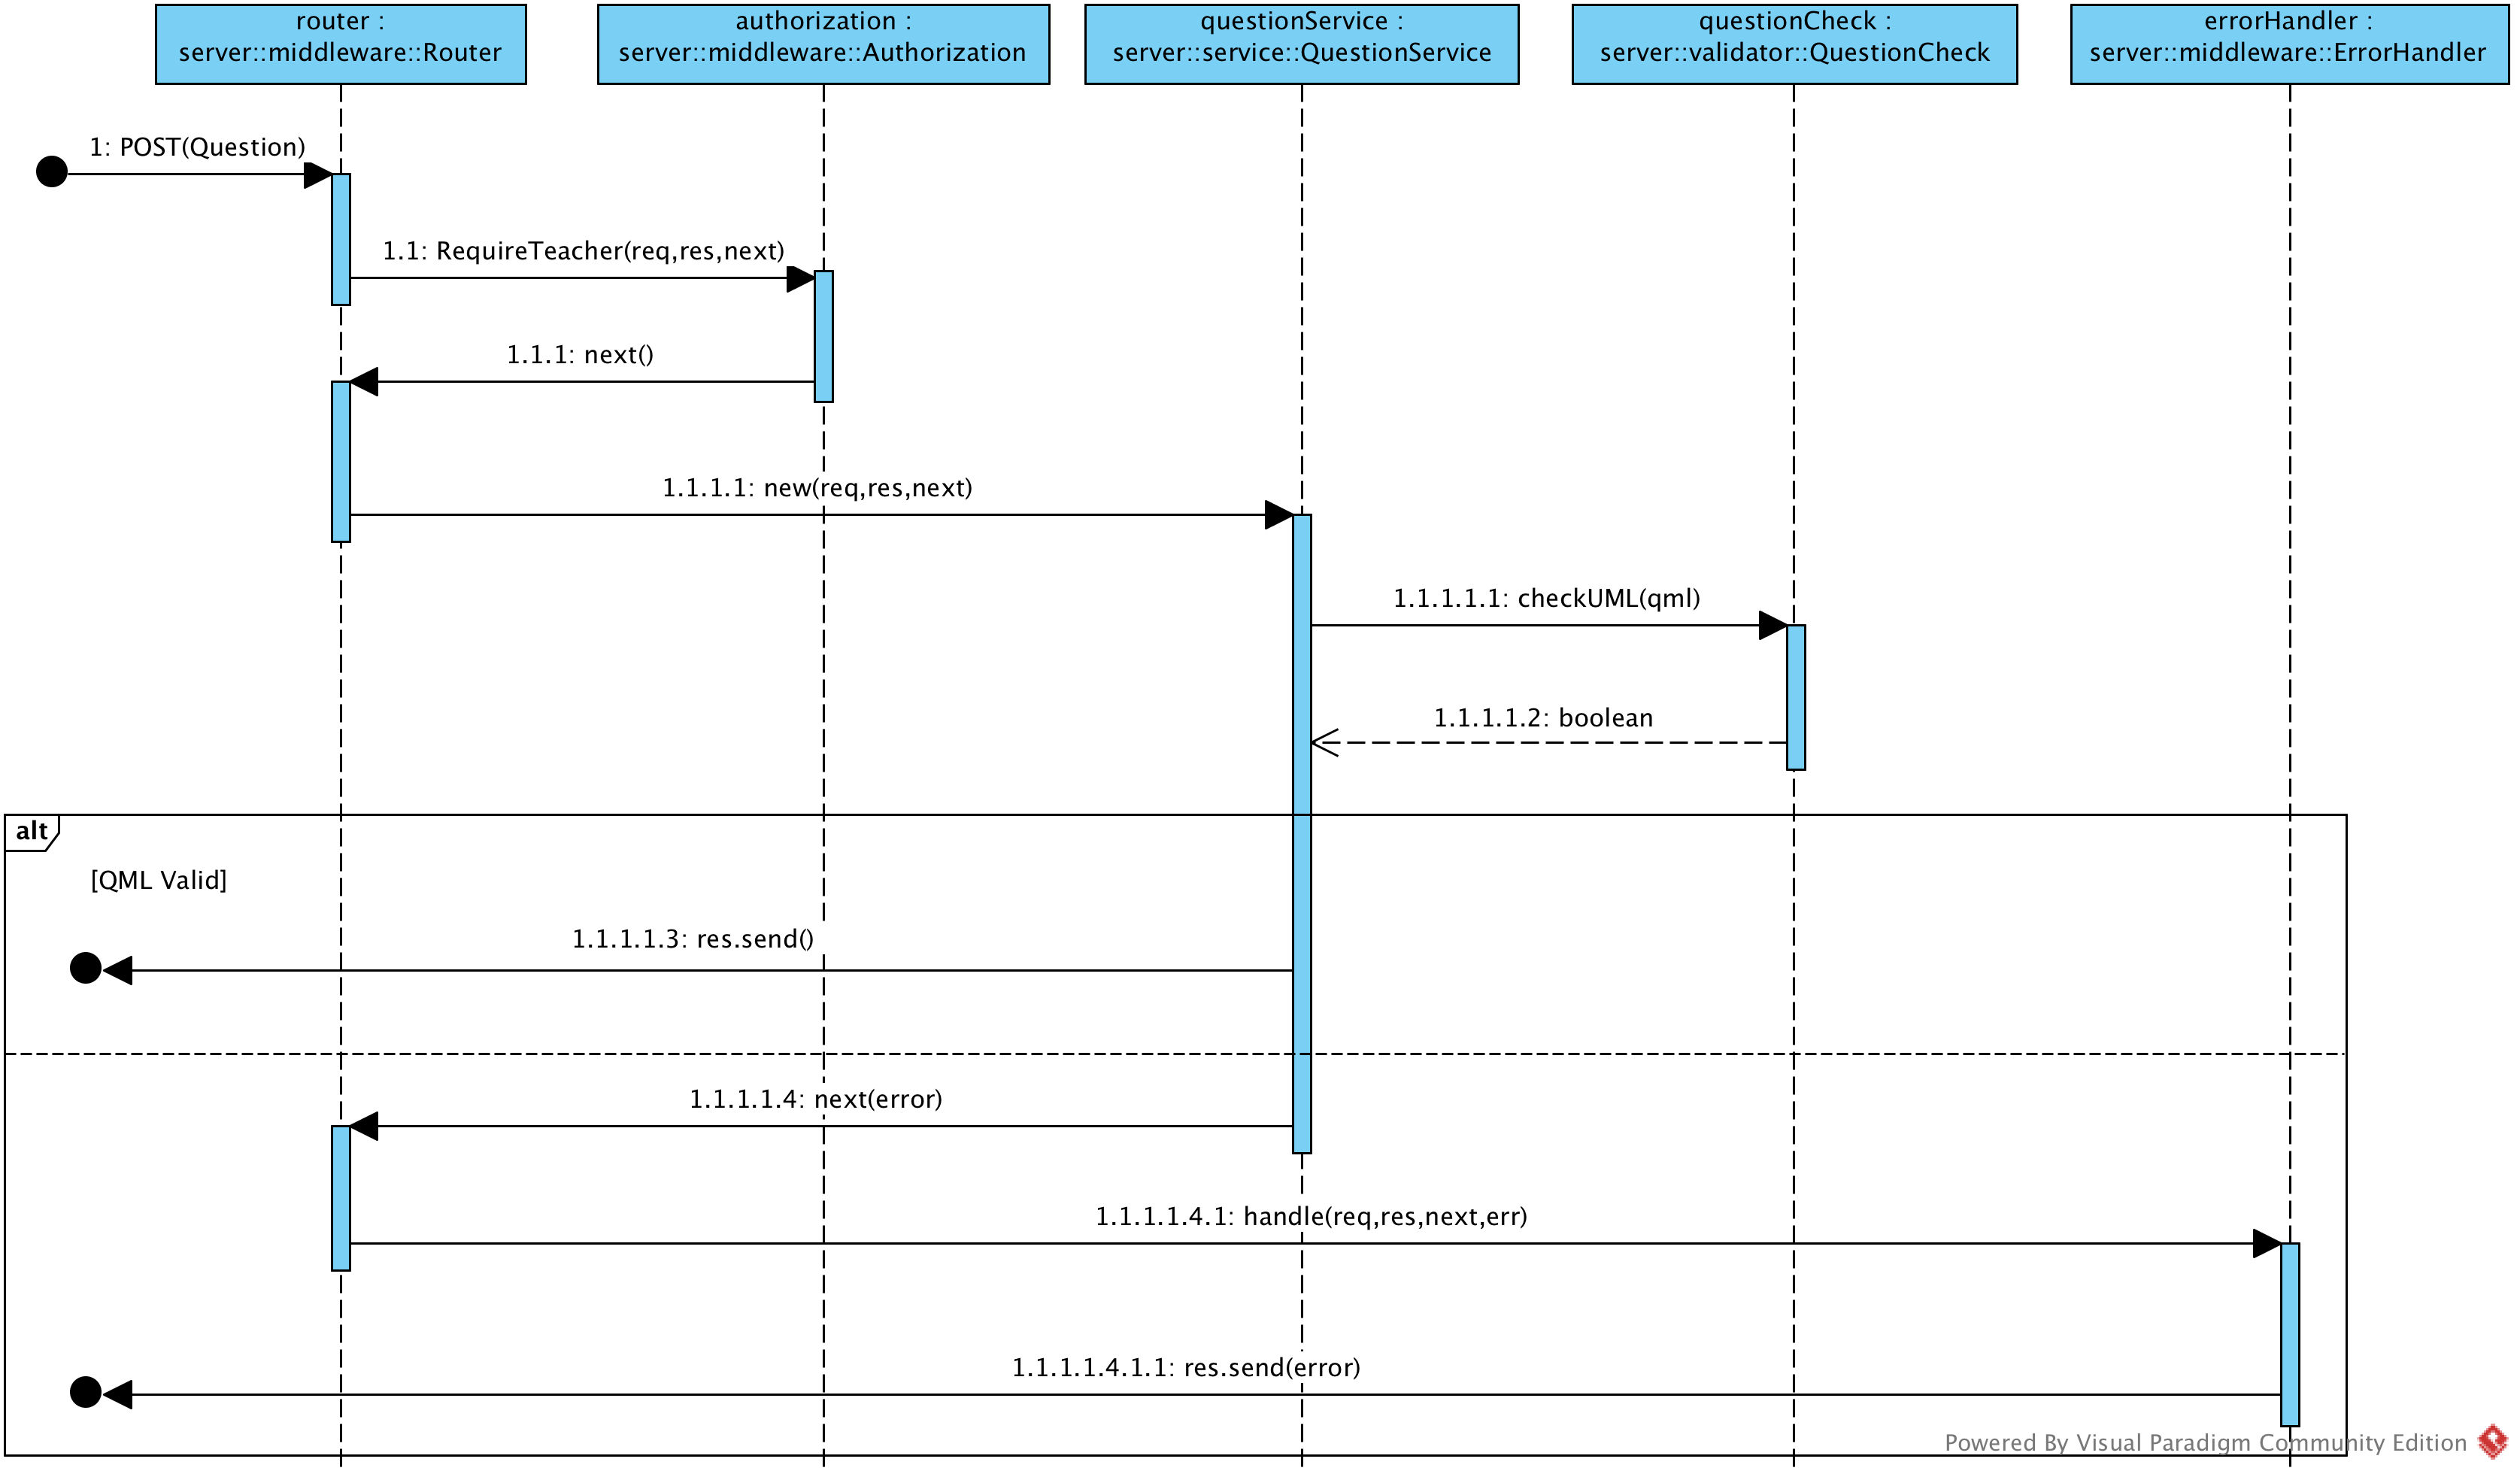
\includegraphics[max width=\myheight, angle=90]{../img/diagrammiSequenza/inserisciDomandaServer.png}
		\caption{Diagramma sequenza - Inserisci Domanda Server}
	\end{figure}
\end{center}

\newpage
\subsubsection{Inserisci Questionario}
Di seguito viene presentato il diagramma di sequenza per l'inserimento di un questionario da parte di un docente, o utente di grado superiore. Gli oggetti e attori attivi durante questa interazione sono:

\begin{itemize}
	\item \textbf{router:} è l'oggetto che si occupa di smistare la richiesta in base all’URI ricevuto e ad invocare l’opportuno servizio
	\item \textbf{authorization:} è l'oggetto che si occupa di verificare i permessi dell'utente per ogni richiesta, in questo caso bisogna che l'utente sia almeno un docente
	\item \textbf{questionnaireService:} è l'oggetto che si occupa di effettuare le modifiche nel database per l'aggiunta del questionario
	\item \textbf{questionnaireCheck:} è l'oggetto che si occupa di controllare che gli attributi di un questionario siano consistenti
	\item \textbf{errorHandler:} è il \mgls{middleware} che viene invocato verso la fine della richiesta che si occupa di trasformare eventuali errori nel formato \mgls{json} richiesto. Viene invocato nel caso in cui la richiesta non sia corretta, se mancano il titolo, gli argomenti o le domande
\end{itemize}

\begin{center}
	\begin{figure}[H]
		\centering 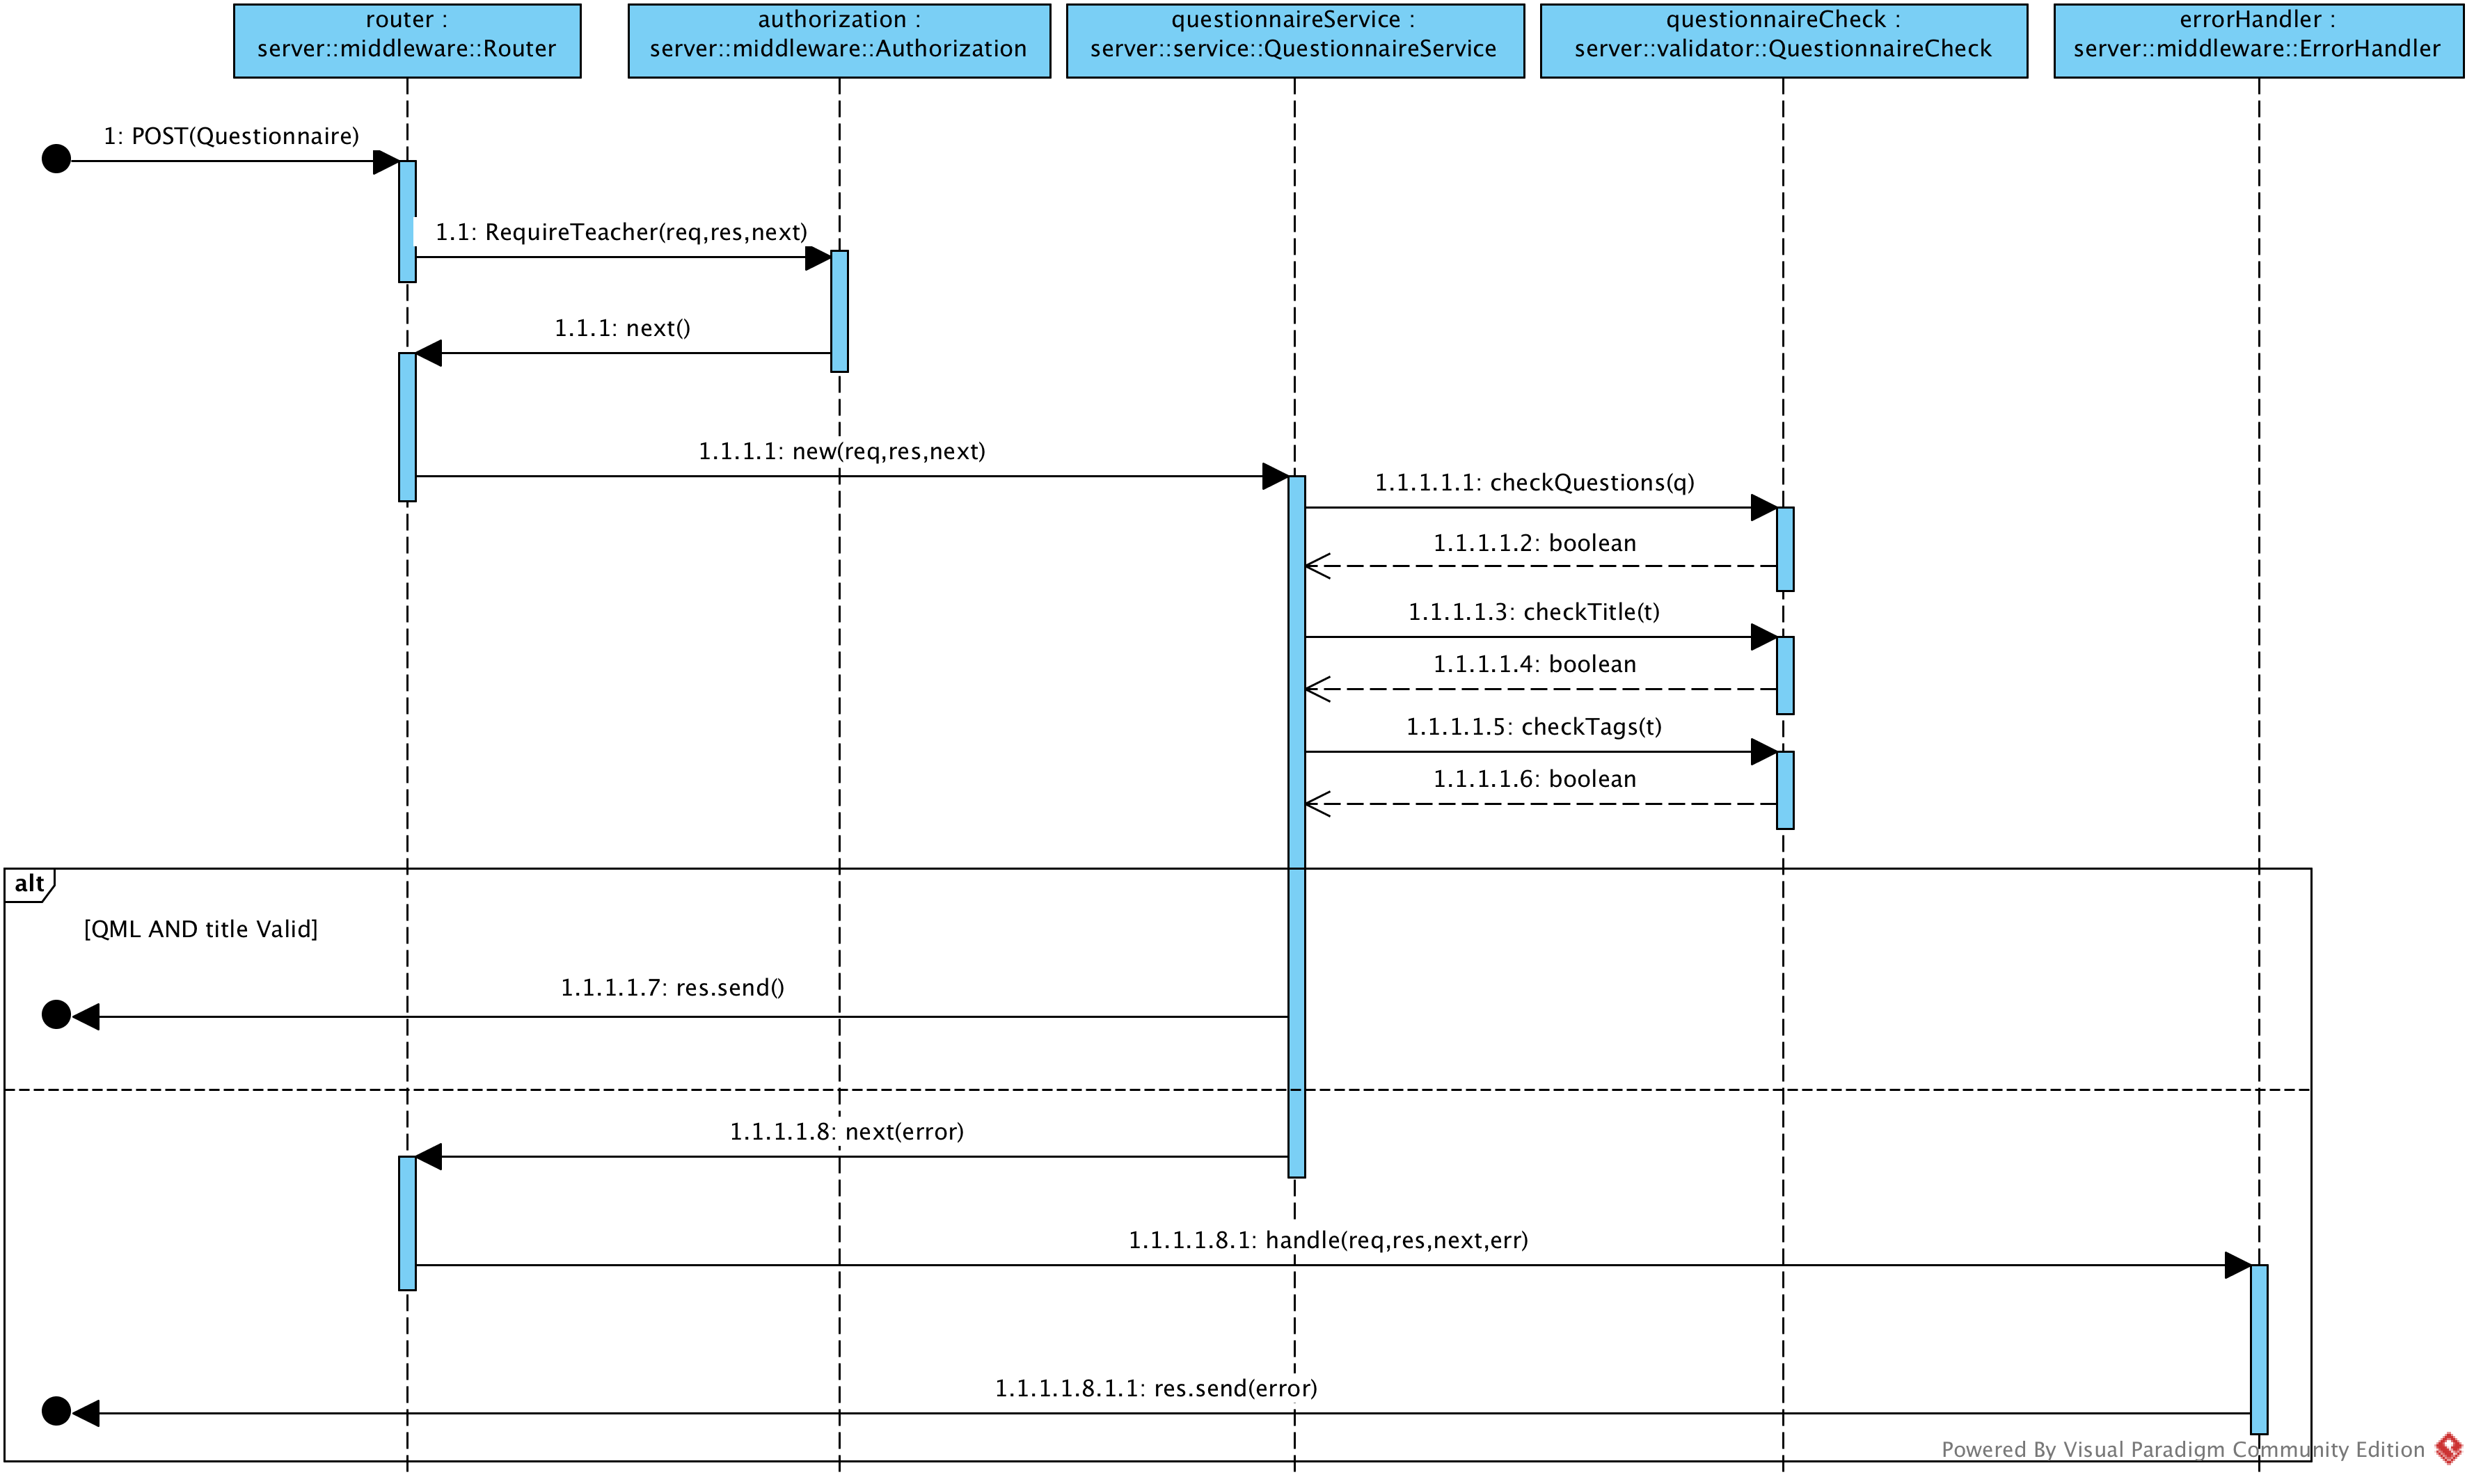
\includegraphics[max width=\myheight, angle=90]{../img/diagrammiSequenza/inserisciQuestionarioServer.png}
		\caption{Diagramma sequenza - Inserisci Questionario Server}
	\end{figure}
\end{center}

\newpage
\subsubsection{Visualizzazione Questionario}
Di seguito viene presentato il diagramma di sequenza per ottenere i dati di un questionario da visualizzare da parte del client. Gli oggetti e attori attivi durante questa interazione sono:

\begin{itemize}
	\item \textbf{router:} è l'oggetto che si occupa di smistare la richiesta in base all’\mgls{uri} ricevuto e ad invocare l’opportuno servizio
	\item \textbf{authorization:} è l'oggetto che si occupa di verificare i permessi dell'utente per ogni richiesta, in questo caso verifica che l'utente sia loggato
	\item \textbf{questionnaireService:} è l'oggetto che si occupa di reperire i dati del questionario da restituire
	\item \textbf{errorHandler:} è il \mgls{middleware} che viene invocato verso la fine della richiesta che si occupa di trasformare eventuali errori nel formato \mgls{json} richiesto. Viene invocato nel caso in cui la richiesta non sia corretta, per esempio quando il questionario selezionato non esiste
\end{itemize}

\begin{center}
	\begin{figure}[H]
		\centering 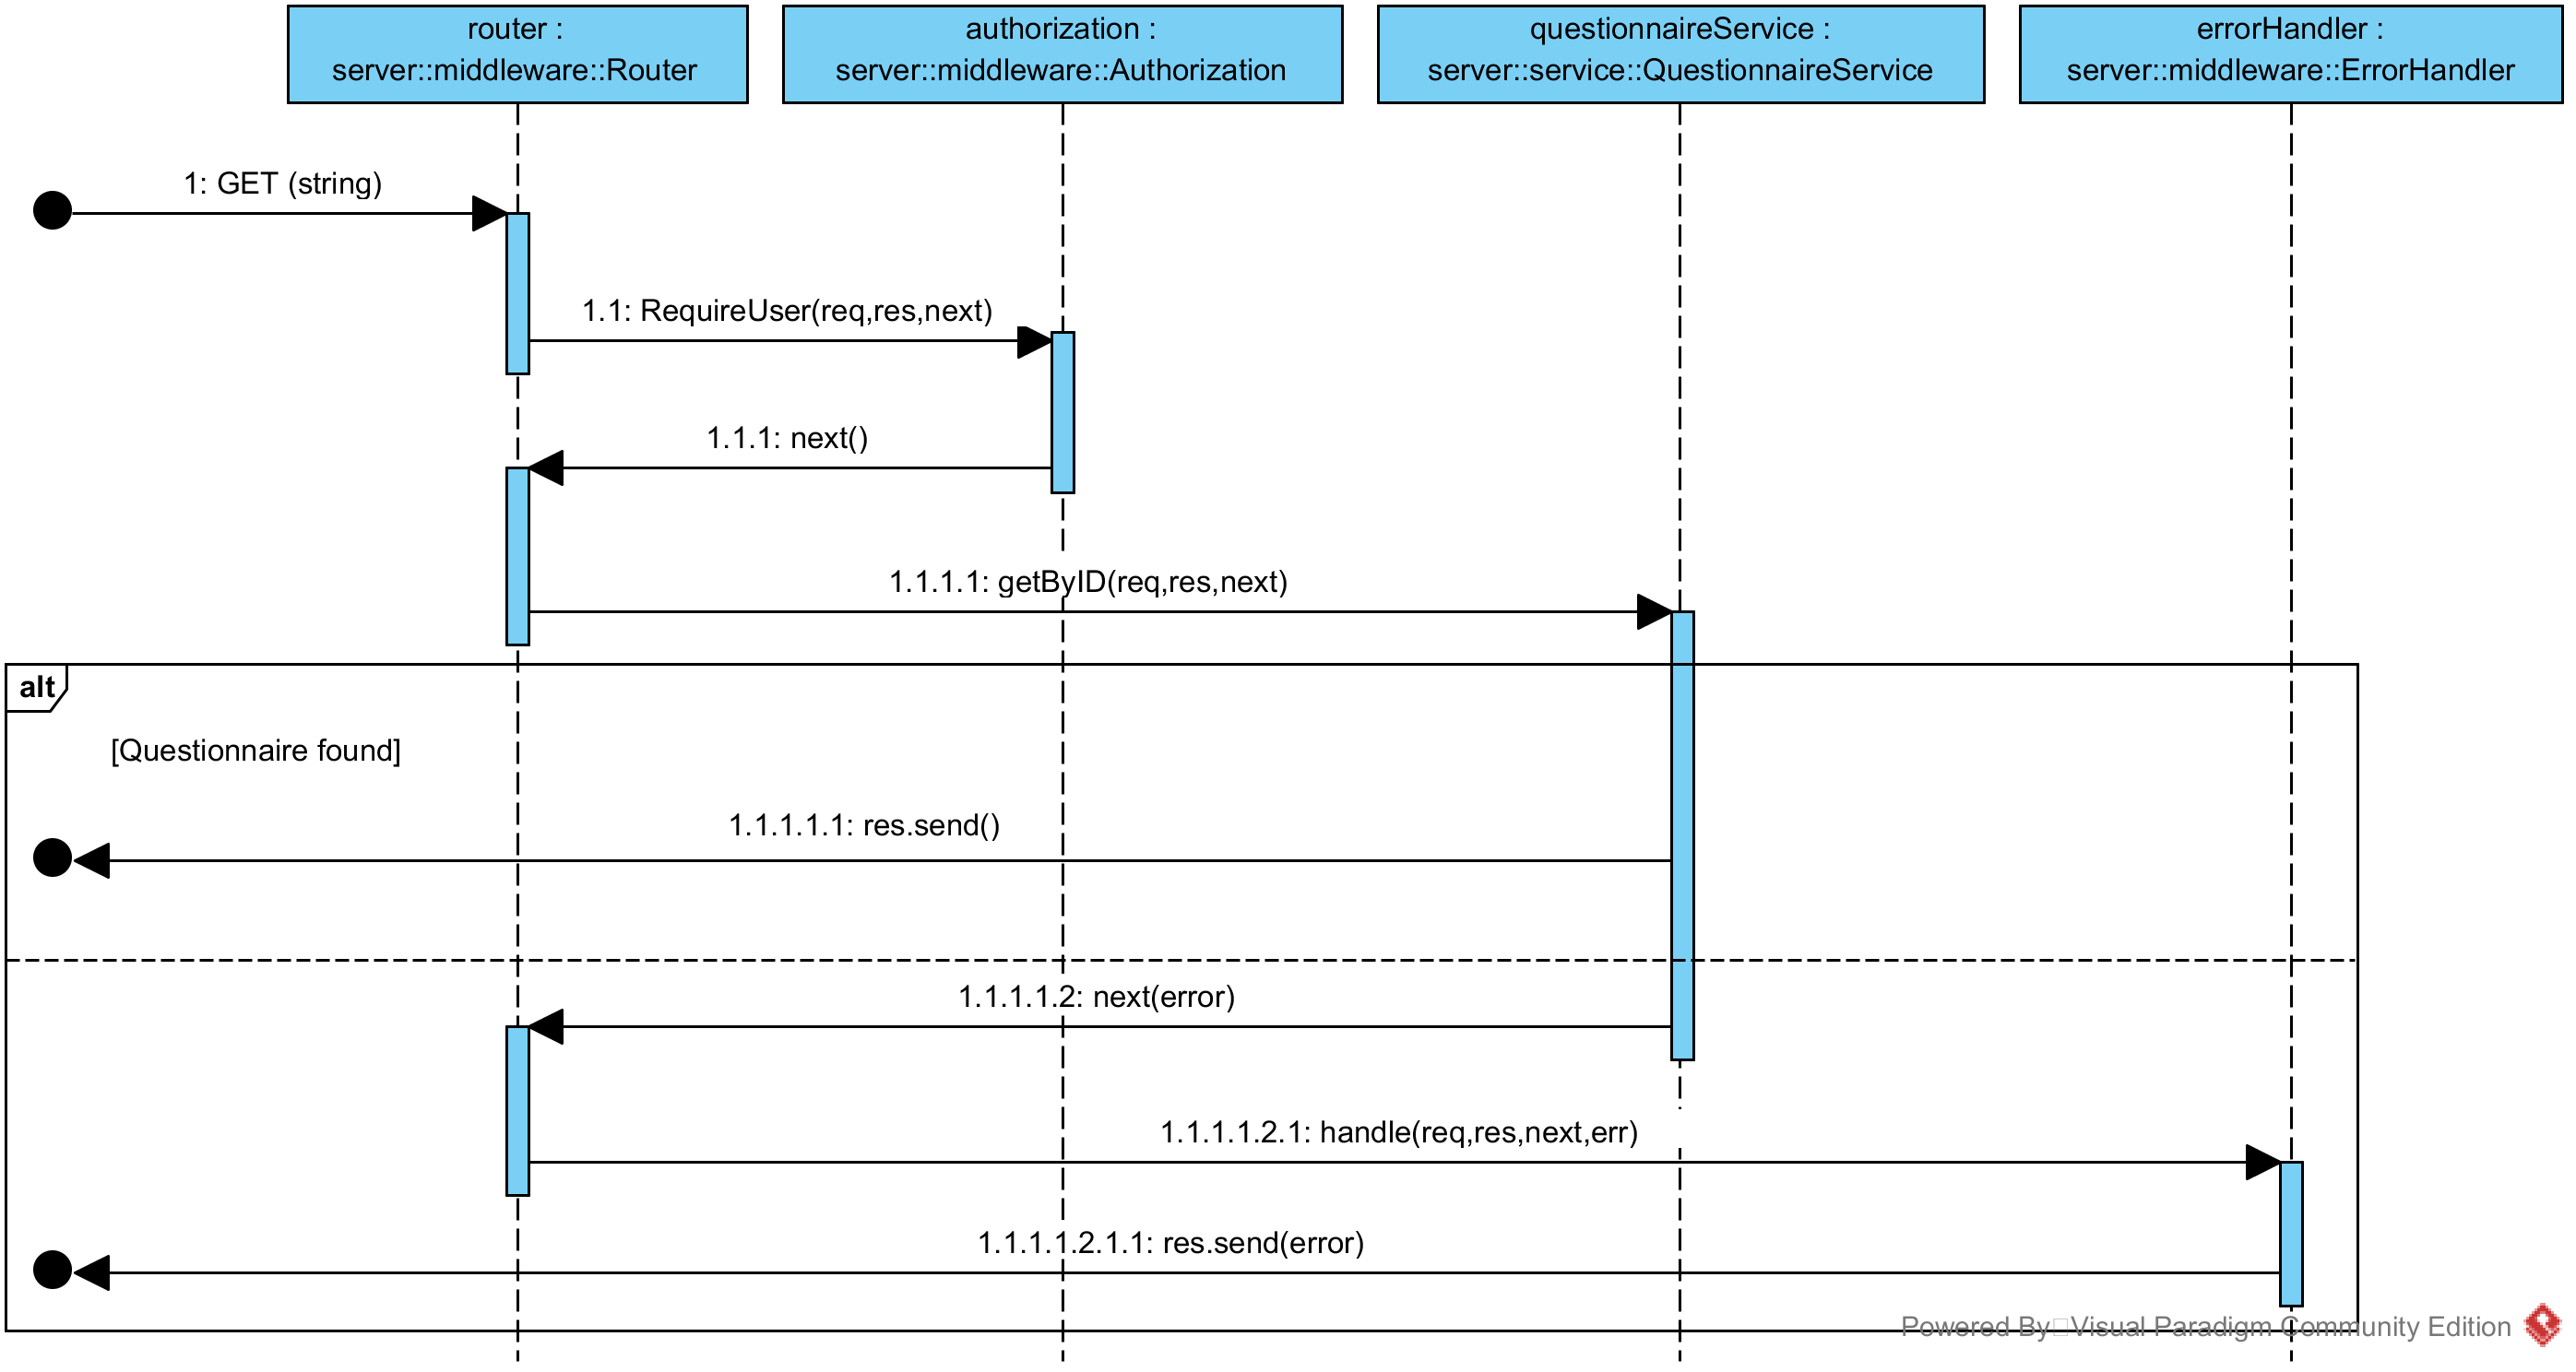
\includegraphics[max width=\myheight, angle=90]{../img/diagrammiSequenza/getQuestionnareDaEseguireServer.png}
		\caption{Diagramma sequenza - Visualizzazione questionario Server}
	\end{figure}
\end{center}

\newpage
\subsubsection{Modifica Domanda}
Di seguito viene presentato il diagramma di sequenza del flusso per la modifica di una domanda da parte del docente, o utente di grado superiore, che l' ha creata. Gli oggetti e attori attivi durante questa interazione sono:

\begin{itemize}
	\item \textbf{router:} è l'oggetto che si occupa di smistare la richiesta in base all’URI ricevuto e ad invocare l’opportuno servizio
	\item \textbf{authorization:} è l'oggetto che si occupa di verificare i permessi dell'utente per ogni richiesta, in questo caso verifica che l'utente sia almeno un docente
	\item \textbf{questionService:} è l'oggetto che si occupa di effettuare le modifiche nel database per la modifica della domanda
	\item \textbf{questionCheck:} è l'oggetto che si occupa di controllare che gli attributi di una domanda siano consistenti
	\item \textbf{errorHandler:} è il \mgls{middleware} che viene invocato verso la fine della richiesta che si occupa di trasformare eventuali errori nel formato \mgls{json} richiesto. Viene invocato nel caso in cui la richiesta non sia corretta, per esempio quando la domanda modificata non ha il QML valido
\end{itemize}

\begin{center}
	\begin{figure}[H]
		\centering 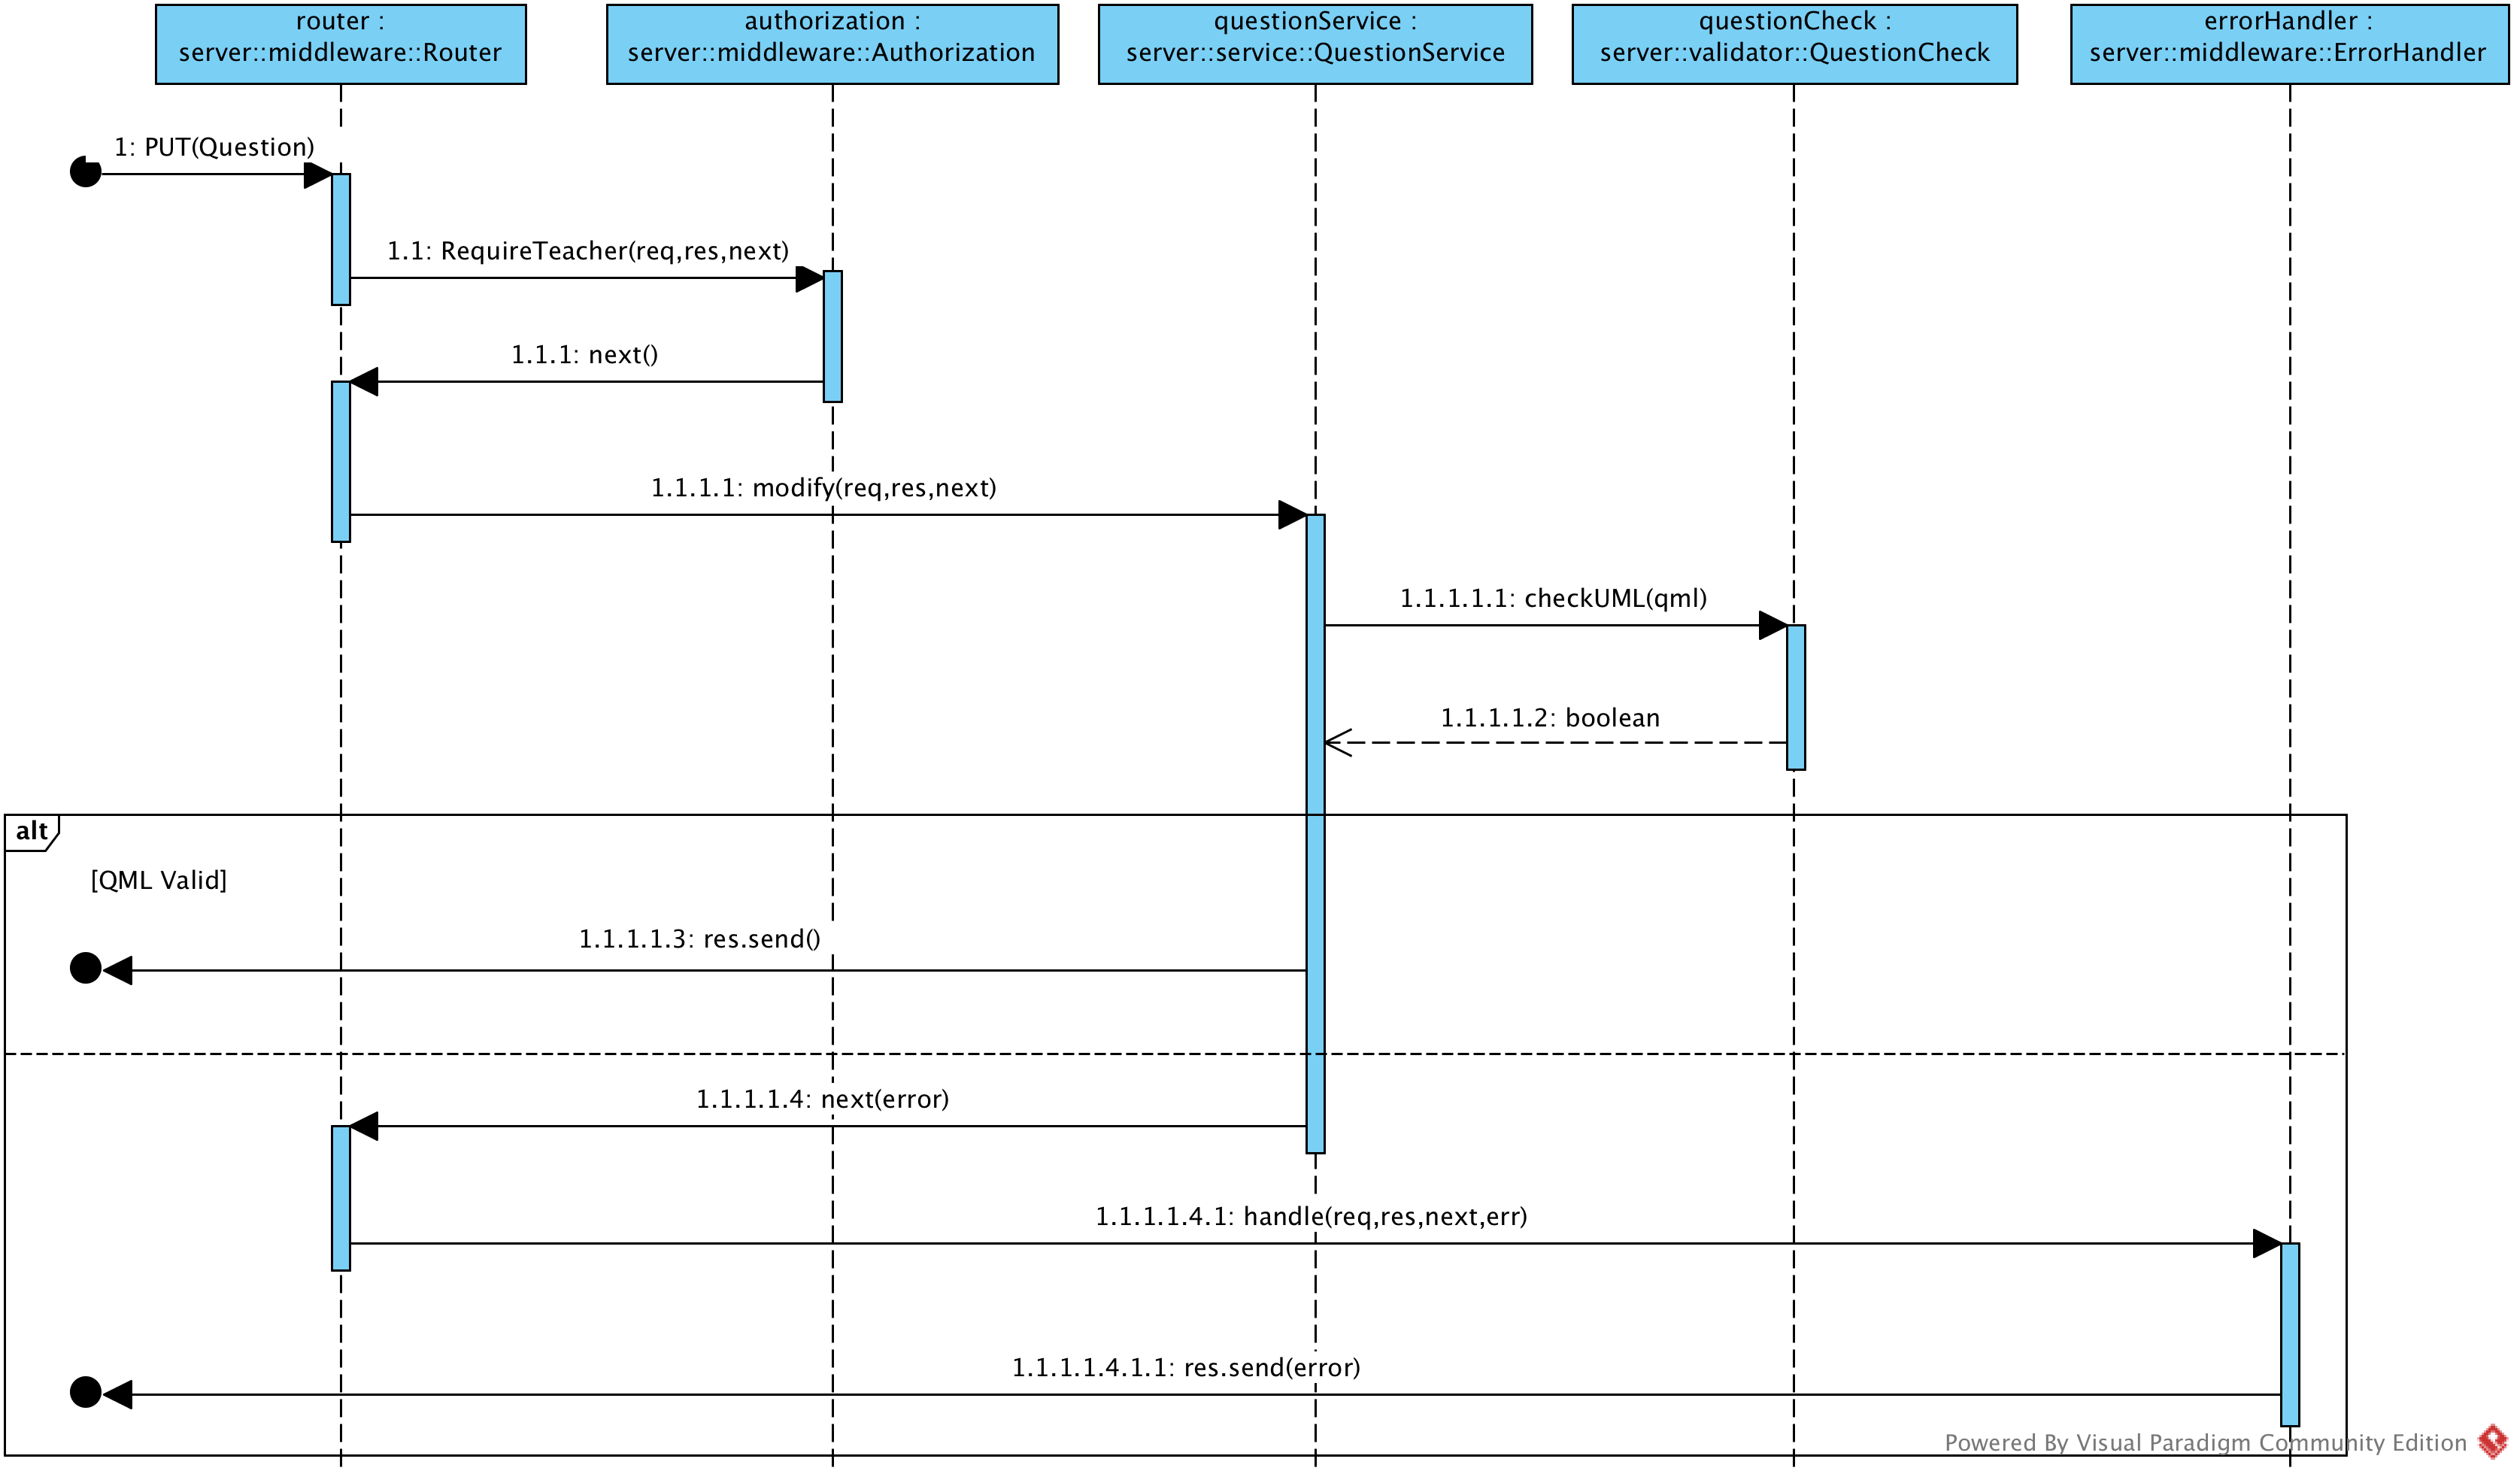
\includegraphics[max width=\myheight, angle=90]{../img/diagrammiSequenza/modificaDomandaServer.png}
		\caption{Diagramma sequenza - Modifica Domanda Server}
	\end{figure}
\end{center}

\newpage
\subsubsection{Modifica Questionario}
Di seguito viene presentato il diagramma di sequenza del flusso per la modifica di un questionario da parte del docente, o utente di grado superiore, che lo ha creato. Gli oggetti e attori attivi durante questa interazione sono:

\begin{itemize}
	\item \textbf{router:} è l'oggetto che si occupa di smistare la richiesta in base all’URI ricevuto e ad invocare l’opportuno servizio
	\item \textbf{authorization:} è l'oggetto che si occupa di verificare i permessi dell'utente per ogni richiesta, in questo caso verifica che l'utente sia almeno un docente
	\item \textbf{questionnaireService:} è l'oggetto che si occupa di effettuare le modifiche nel database per la modifica del questionario
	\item \textbf{questionnaireCheck:} è l'oggetto che si occupa di controllare che gli attributi di un questionario siano consistenti
	\item \textbf{errorHandler:} è il \mgls{middleware} che viene invocato verso la fine della richiesta che si occupa di trasformare eventuali errori nel formato \mgls{json} richiesto. Viene invocato nel caso in cui la richiesta non sia corretta, per esempio quando il nuovo questionario non presenta titolo, argomenti o domande
\end{itemize}

\begin{center}
	\begin{figure}[H]
		\centering 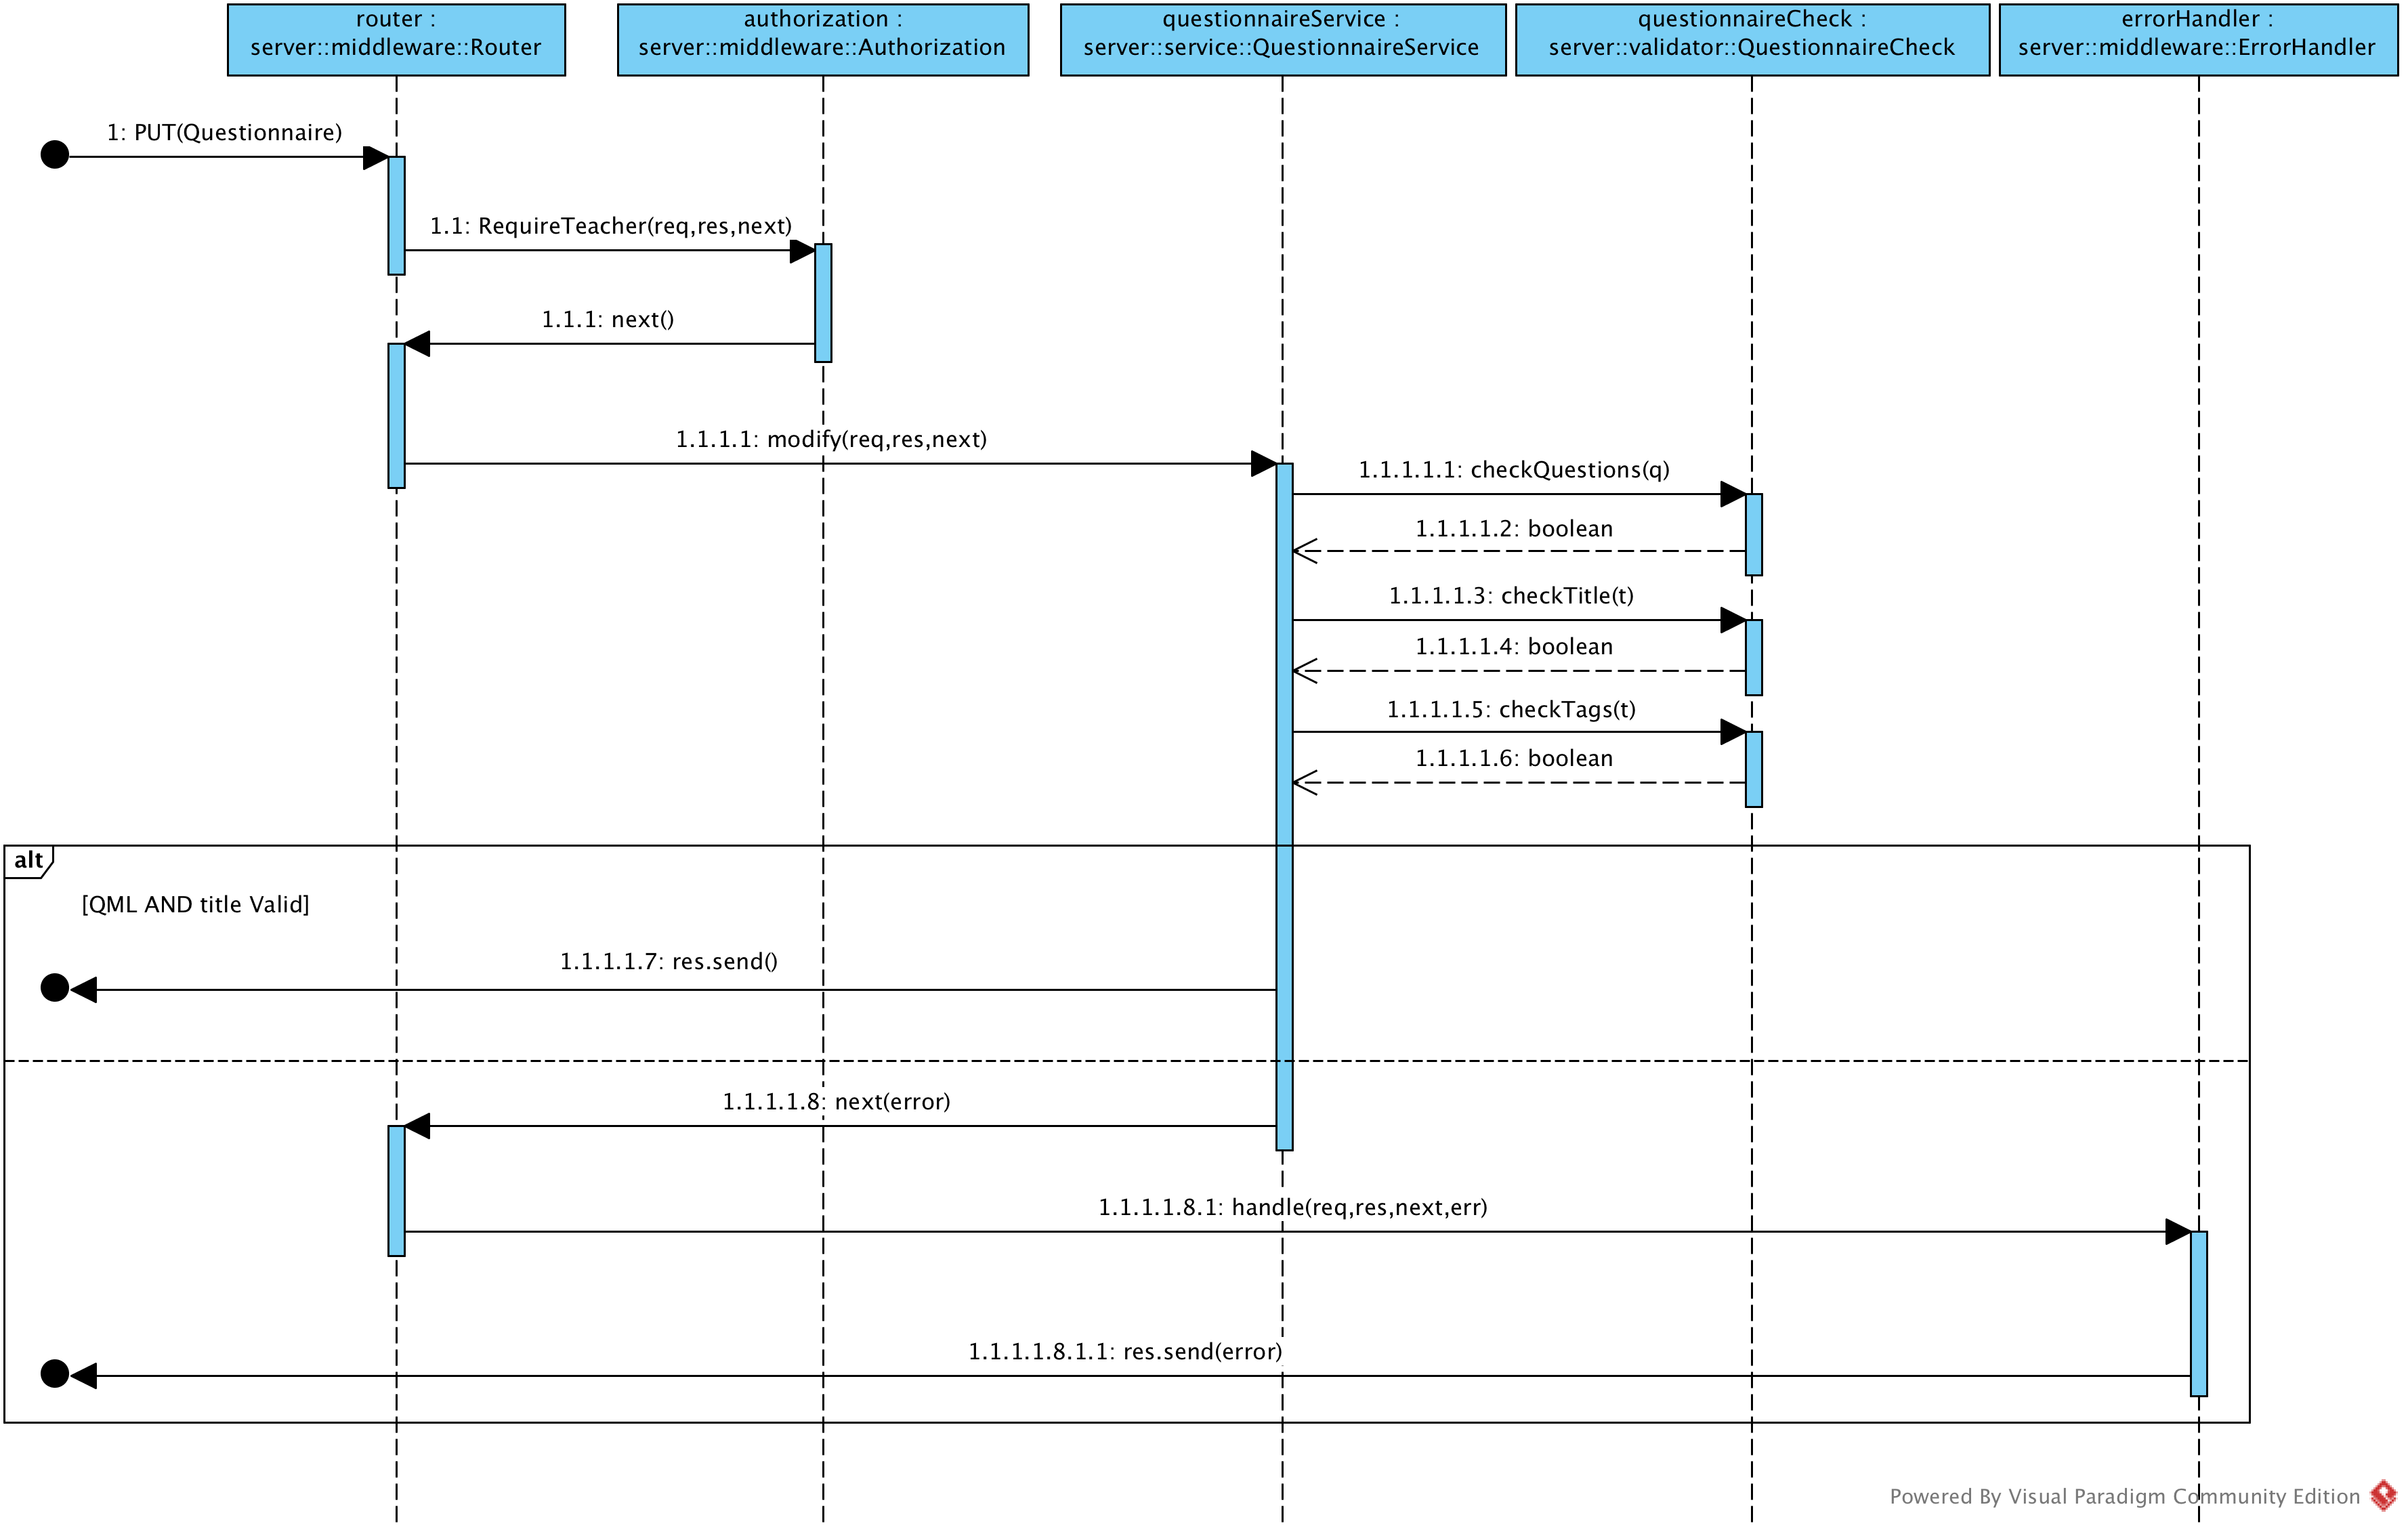
\includegraphics[max width=\myheight, angle=90]{../img/diagrammiSequenza/modificaQuestionarioServer.png}
		\caption{Diagramma sequenza - Modifica Questionario Server}
	\end{figure}
\end{center}

\newpage
\subsubsection{Rimozione Domanda}
Di seguito viene presentato il diagramma di sequenza del flusso per la rimozione di una domanda da parte del docente, o utente di grado superiore, che la ha creata. Gli oggetti e attori attivi durante questa interazione sono:

\begin{itemize}
	\item \textbf{router:} è l'oggetto che si occupa di smistare la richiesta in base all’URI ricevuto e ad invocare l’opportuno servizio
	\item \textbf{authorization:} è l'oggetto che si occupa di verificare i permessi dell'utente per ogni richiesta, in questo caso si verifica che l'utente sia almeno un docente
	\item \textbf{questionService:} è l'oggetto che si occupa di effettuare le modifiche nel database per la rimozione della domanda
	\item \textbf{errorHandler:} è il \mgls{middleware} che viene invocato verso la fine della richiesta che si occupa di trasformare eventuali errori nel formato \mgls{json} richiesto. Viene invocato nel caso in cui la richiesta non sia corretta, per esempio quando il questionario da eliminare non esiste
\end{itemize}

\begin{center}
	\begin{figure}[H]
		\centering 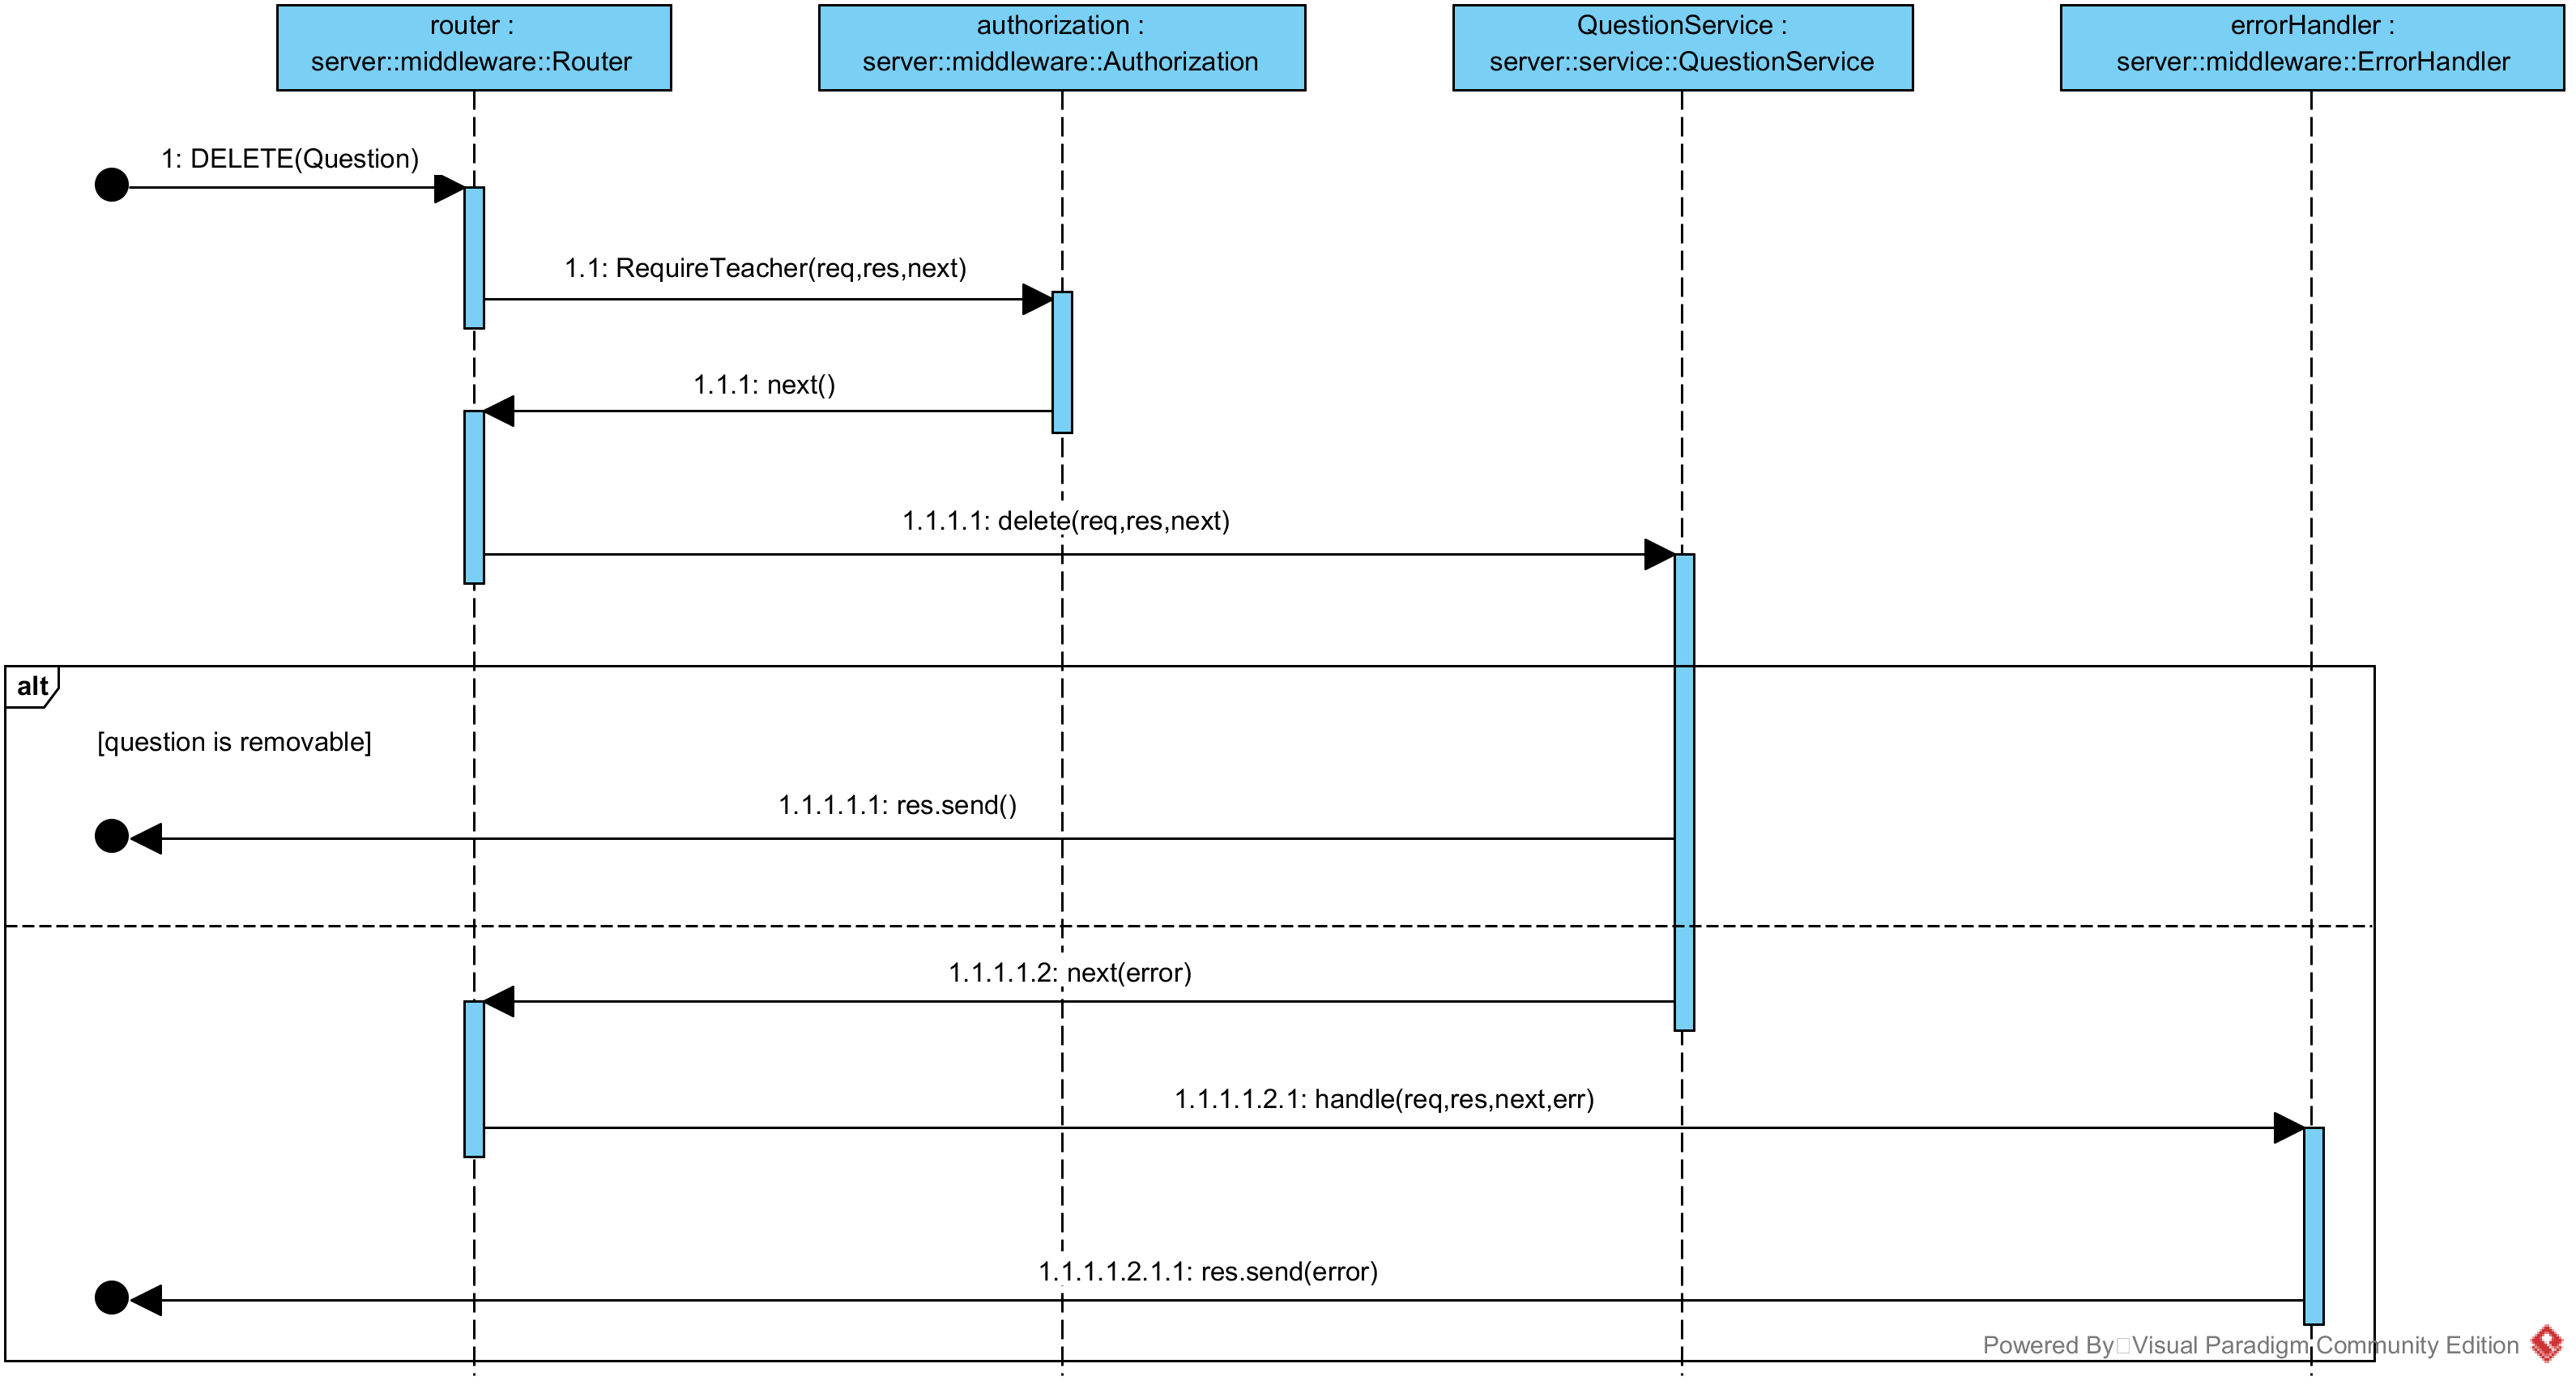
\includegraphics[max width=\myheight, angle=90]{../img/diagrammiSequenza/rimozioneDomandaServer.png}
		\caption{Diagramma sequenza - Rimozione Domanda Server}
	\end{figure}
\end{center}

\newpage
\subsubsection{Rimozione Questionario}
Di seguito viene presentato il diagramma di sequenza del flusso per la rimozione di una questionario da parte del docente, o utente di grado superiore, che lo ha creato. Gli oggetti e attori attivi durante questa interazione sono:

\begin{itemize}
	\item \textbf{router:} è l'oggetto che si occupa di smistare la richiesta in base all’URI ricevuto e ad invocare l’opportuno servizio
	\item \textbf{authorization:} è l'oggetto che si occupa di verificare i permessi dell'utente per ogni richiesta, in questo caso verifica l'utente sia almeno un docente
	\item \textbf{questionnaireService:} è l'oggetto che si occupa di effettuare le modifiche nel database per la rimozione del questionario
	\item \textbf{errorHandler:} è il \mgls{middleware} che viene invocato verso la fine della richiesta che si occupa di trasformare eventuali errori nel formato \mgls{json} richiesto
\end{itemize}

\begin{center}
	\begin{figure}[H]
		\centering 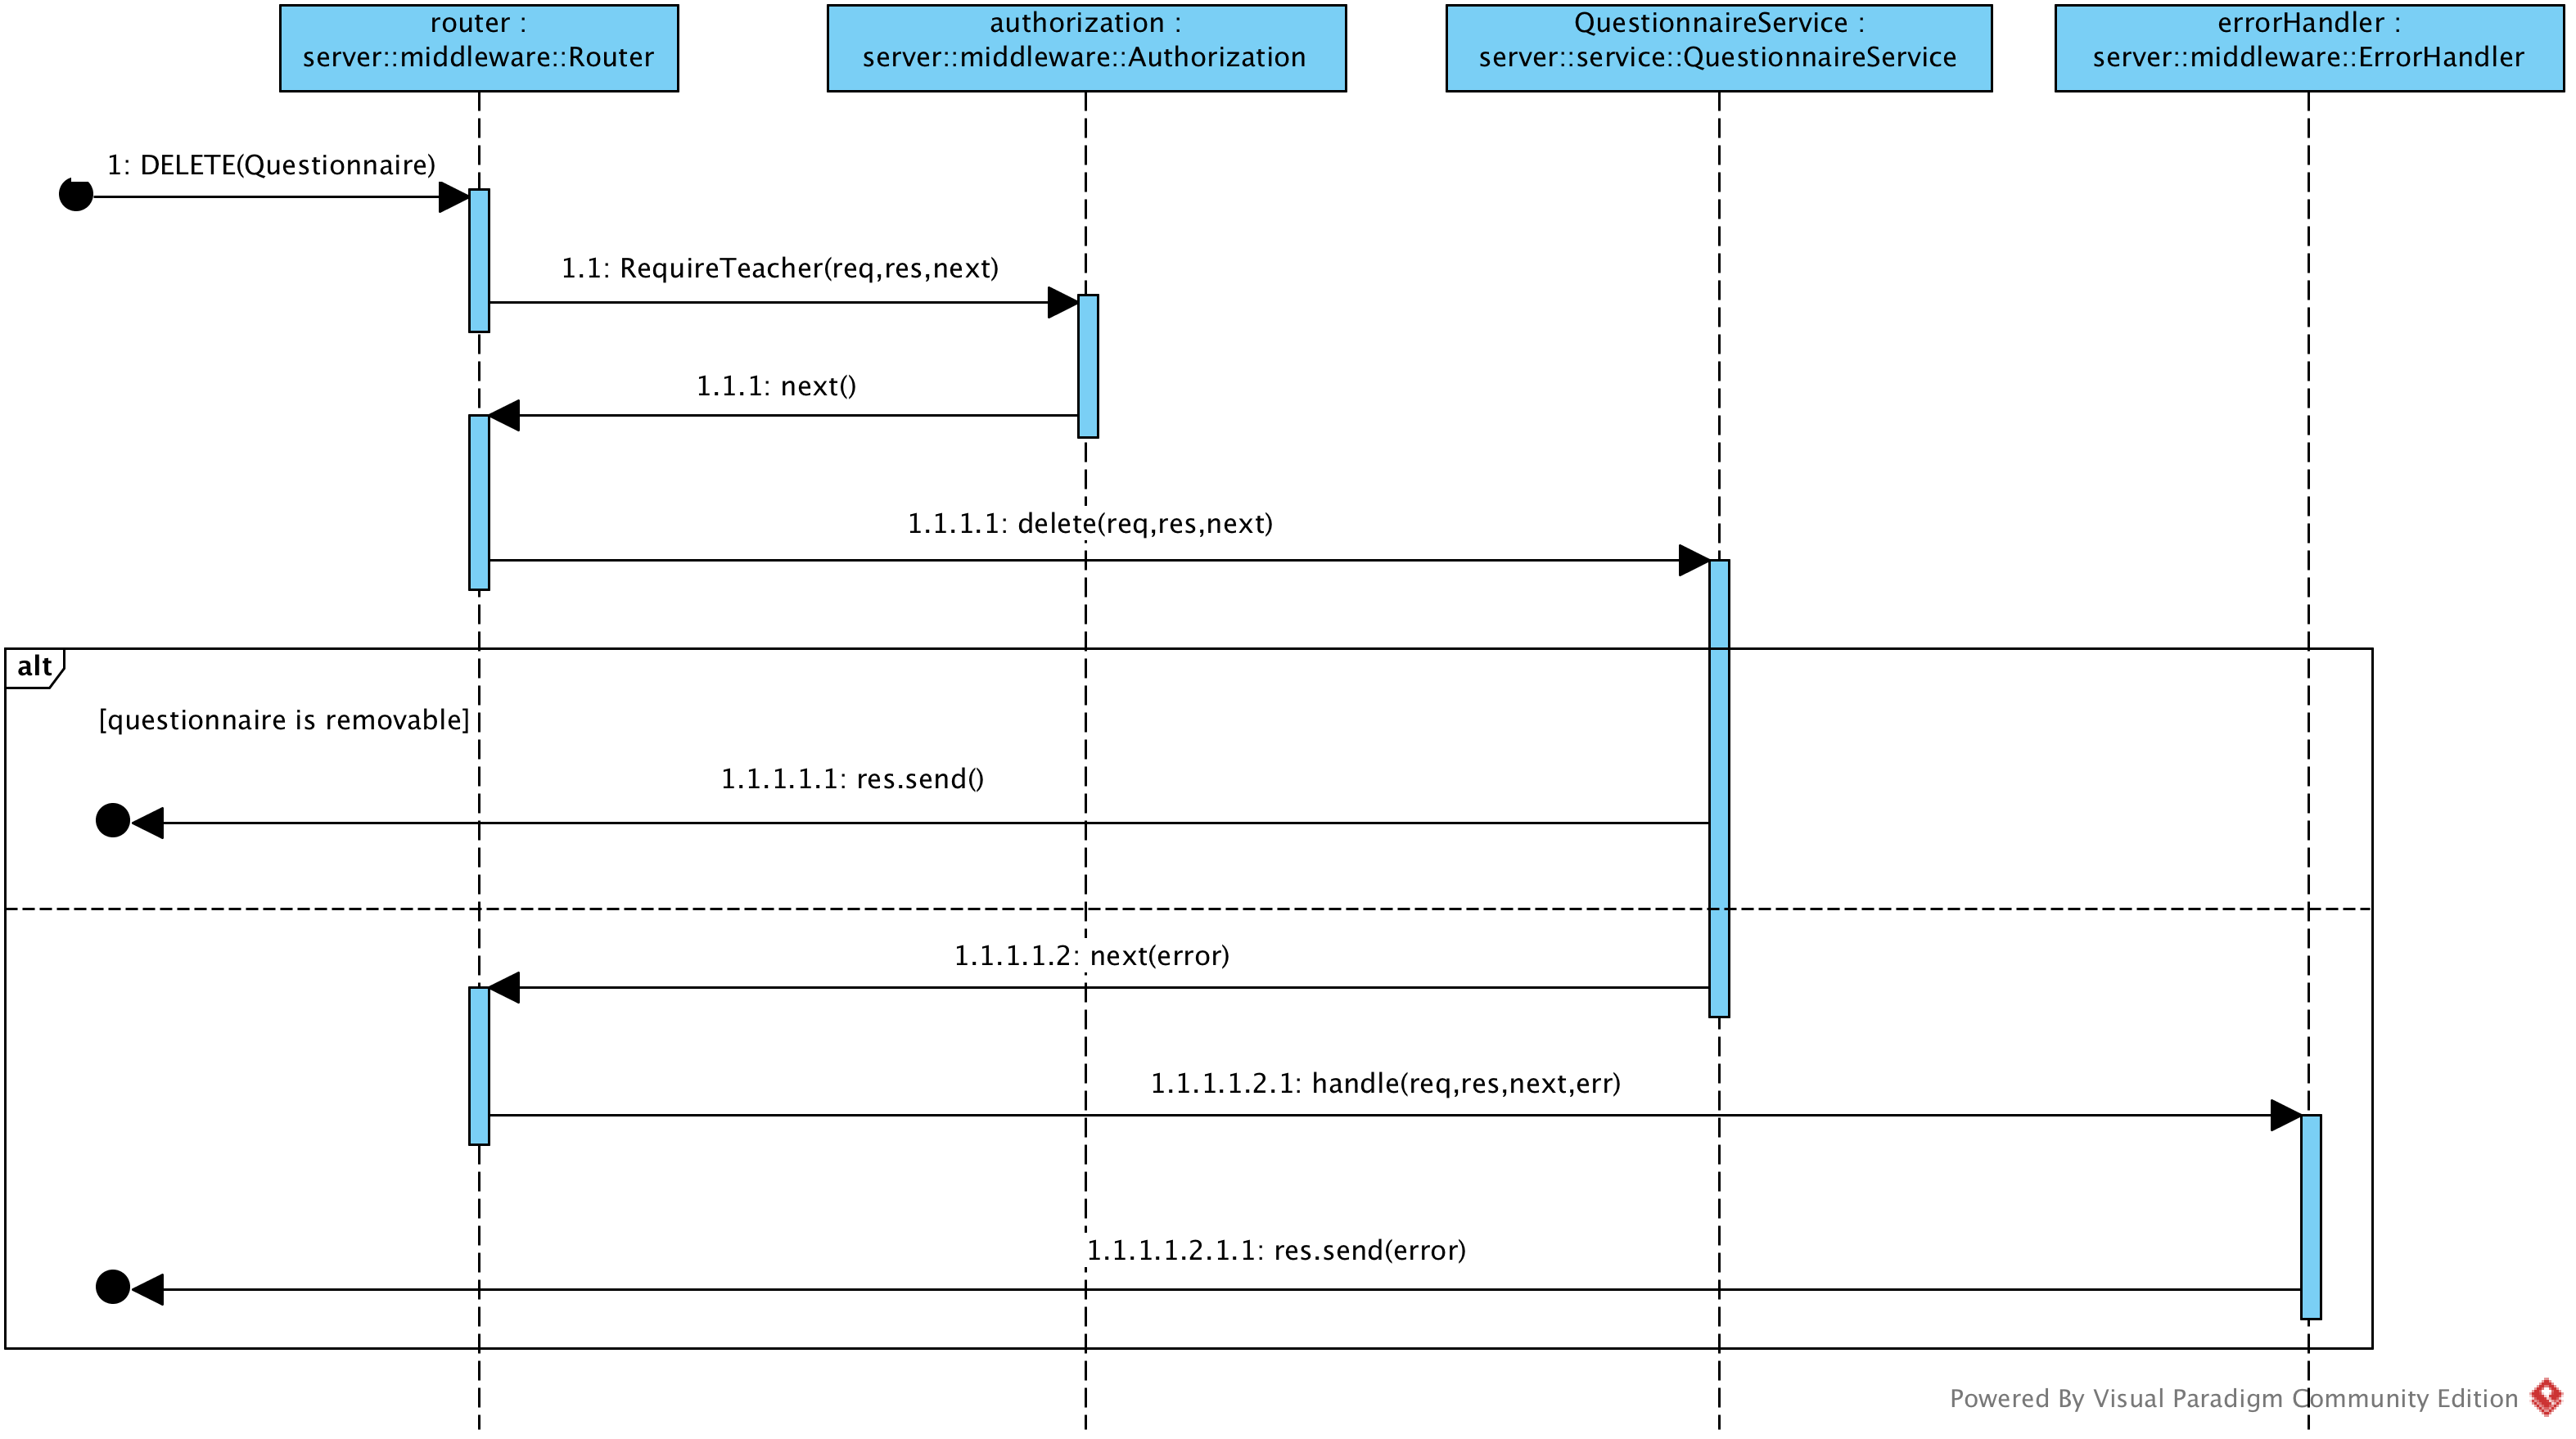
\includegraphics[max width=\myheight, angle=90]{../img/diagrammiSequenza/rimozioneQuestionarioServer.png}
		\caption{Diagramma sequenza - Rimozione Questionario Server}
	\end{figure}
\end{center}

\subsection{Client}

Vengono di seguito presentati i diagrammi di sequenza di alcune delle operazioni più significative lato \mgls{client}, ovvero il front-end dell'applicazione.

\subsubsection{Login}
Di seguito viene presentato il diagramma di sequenza per l'accesso da parte di un ospite dal punto di vista del client. L'utente inserisce le credenziali e chiama submit() sul controller il quale si occuperà di richiamare i servizi adatti per istanziare una nuova sessione. Gli oggetti e attori attivi durante questa interazione sono:

\begin{itemize}
	\item \textbf{Ospite:} l'utente non autenticato che ha intenzione di effettuare l'accesso
	\item \textbf{LogInView:} è la pagina che mostra il form per accedere
	\item \textbf{LogInController:} è il \mgls{controller} dell'applicazione che si occupa di controllare i dati immessi dall'utente e chiamare il servizio per effettuare il login
	\item \textbf{sessionService:} è l'oggetto che invia la richiesta di login al server
	\item \textbf{userService:} è l'oggetto che si occupa di comunicare con il server per ottenere i dati dell'utente autenticato
\end{itemize}

\begin{center}
	\begin{figure}[H]
		\centering 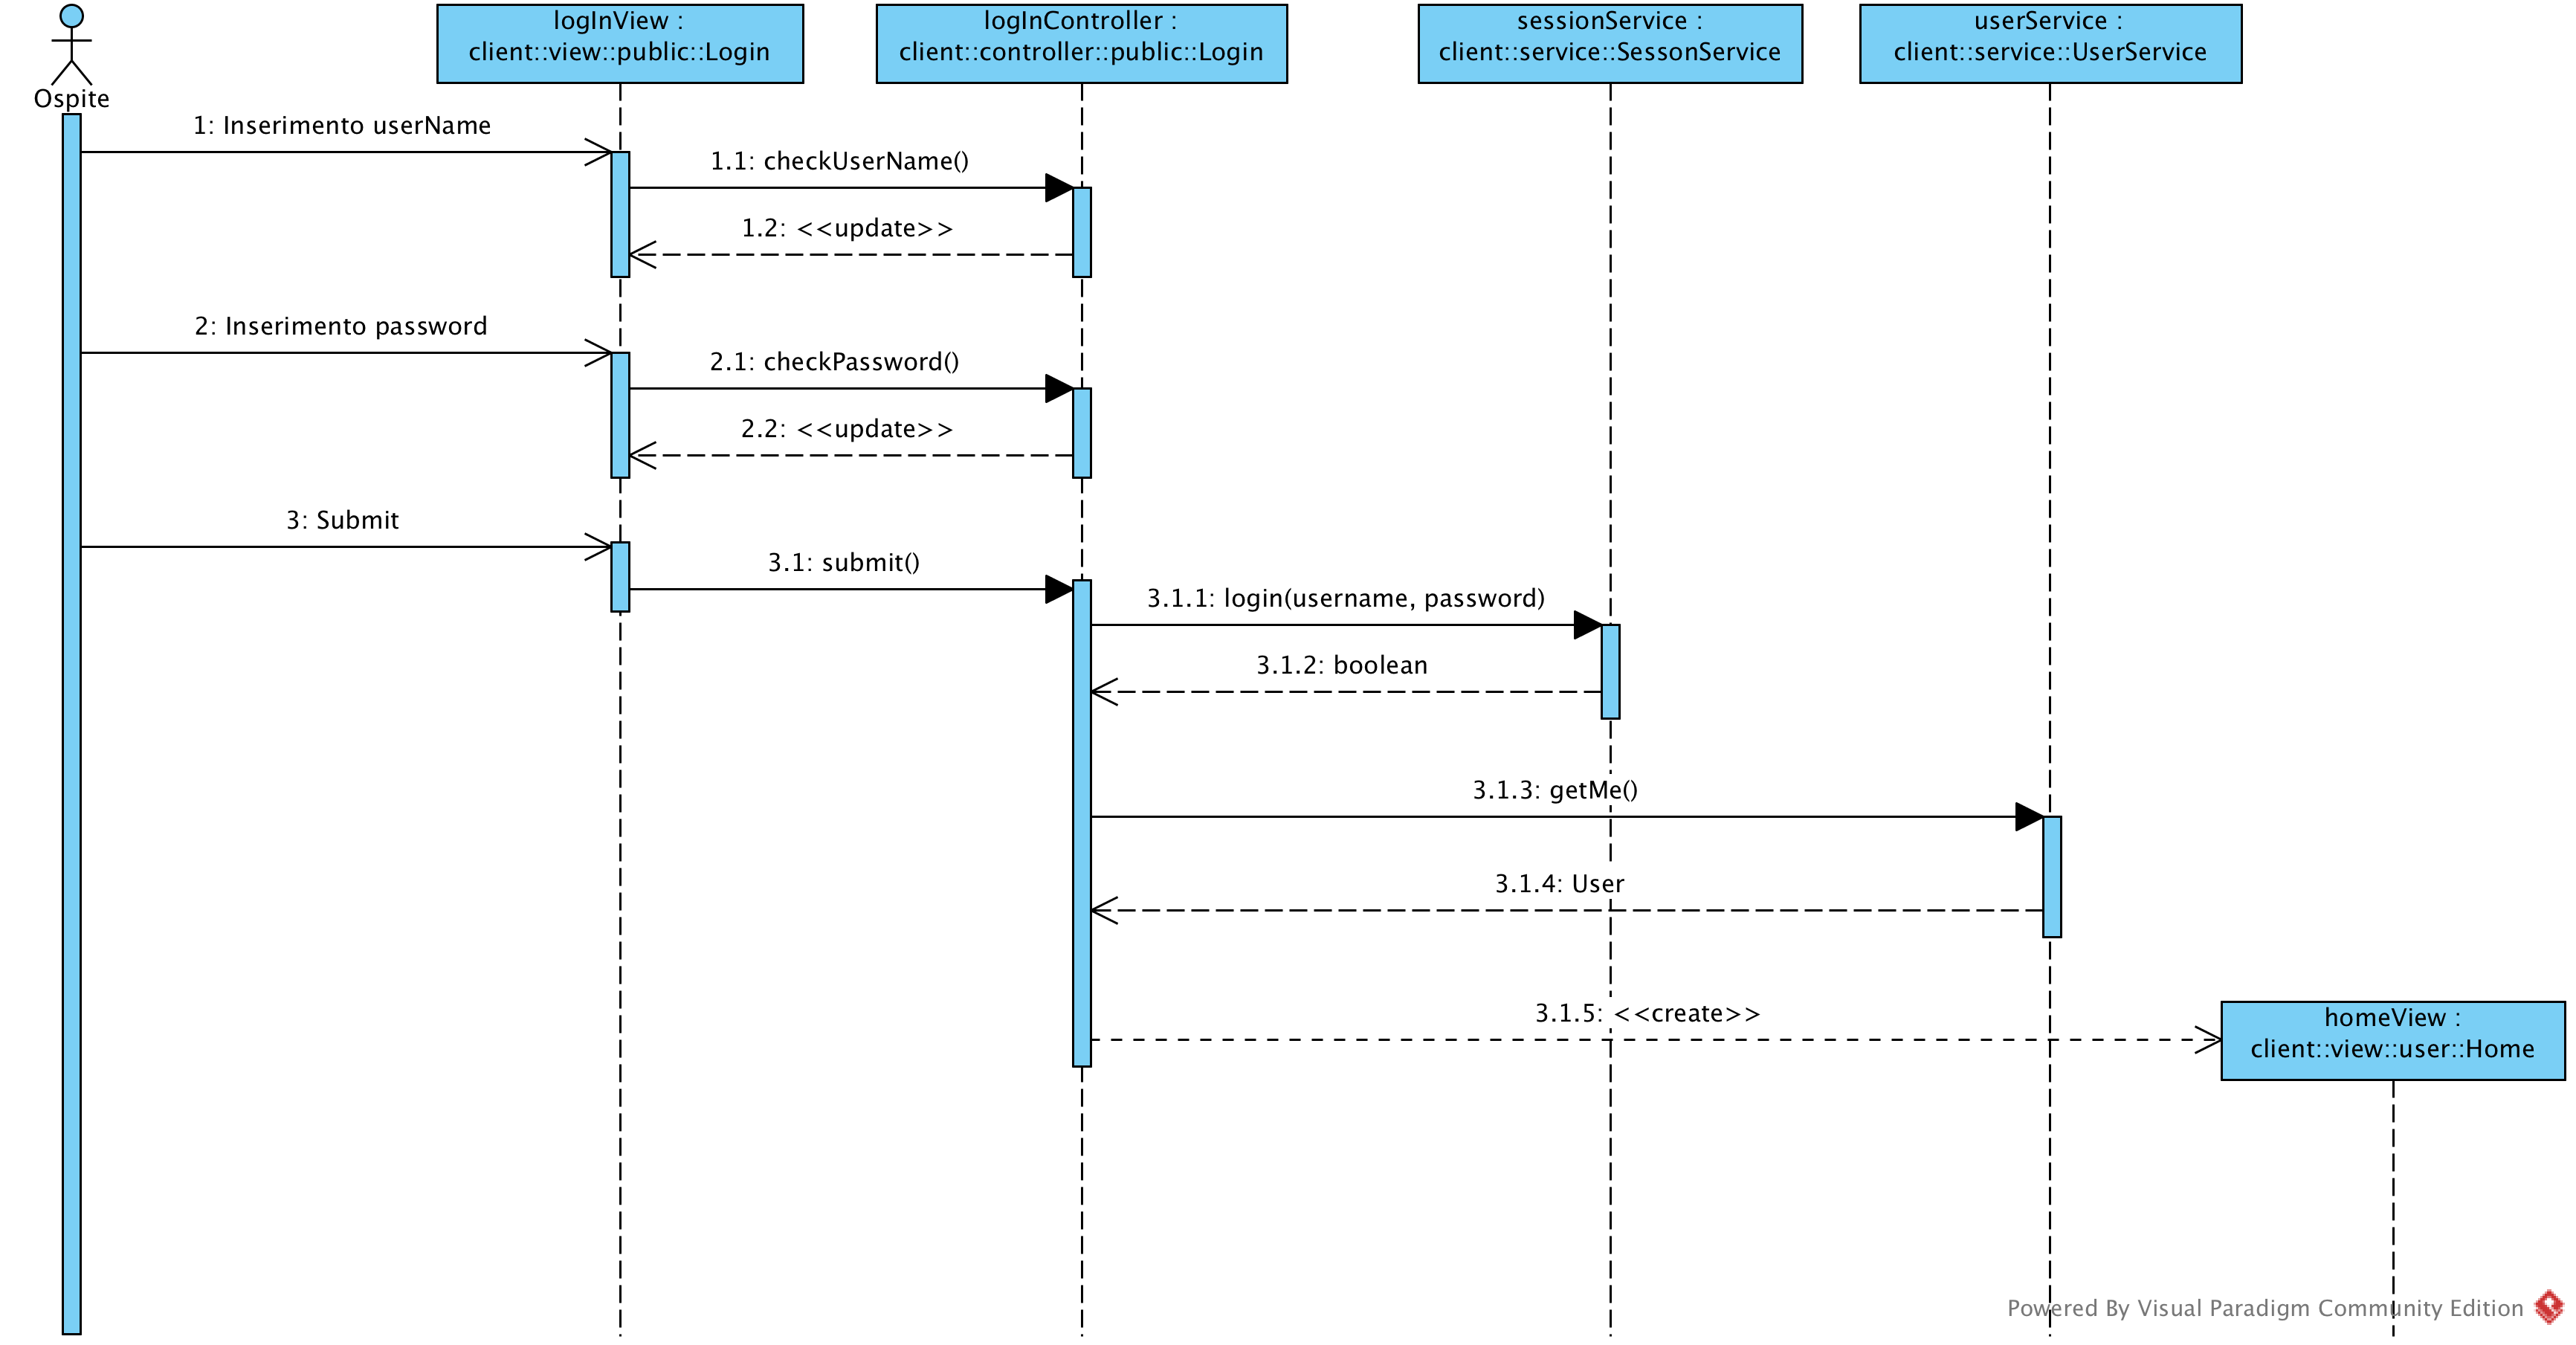
\includegraphics[max width=\myheight, angle=90]{../img/diagrammiSequenza/loginClient.png}
		\caption{Diagramma sequenza - Login Client}
	\end{figure}
\end{center}

\newpage
\subsubsection{Cambio Informazioni}
Di seguito viene presentato il diagramma di sequenza del flusso per il cambio di nome utente e nome completo da parte di un utente autenticato presso il sistema. L'utente inserisce i dati modificati e li invia al controller il quale chiama i servizi adatti per modificare il profilo personale. Gli oggetti e attori attivi durante questa interazione sono:

\begin{itemize}
	\item \textbf{Studente:} l'utente autenticato con ruolo di studente o superiore che ha intenzione di cambiare le informazioni personali
	\item \textbf{userView:} è la pagina che mostra i dati dell'utente connesso al sistema
	\item \textbf{userController:} è il \mgls{controller} dell'applicazione che si occupa delle modifiche dell'utente, dal cambio di informazioni personali al cambio di password
	\item \textbf{check:} è l'oggetto che controlla se la password, l'username o titolo rispettano il formato scelto	
	\item \textbf{userService:} è l'oggetto che si occupa di comunicare con il server per apportare le modifiche
\end{itemize}

\begin{center}
	\begin{figure}[H]
		\centering 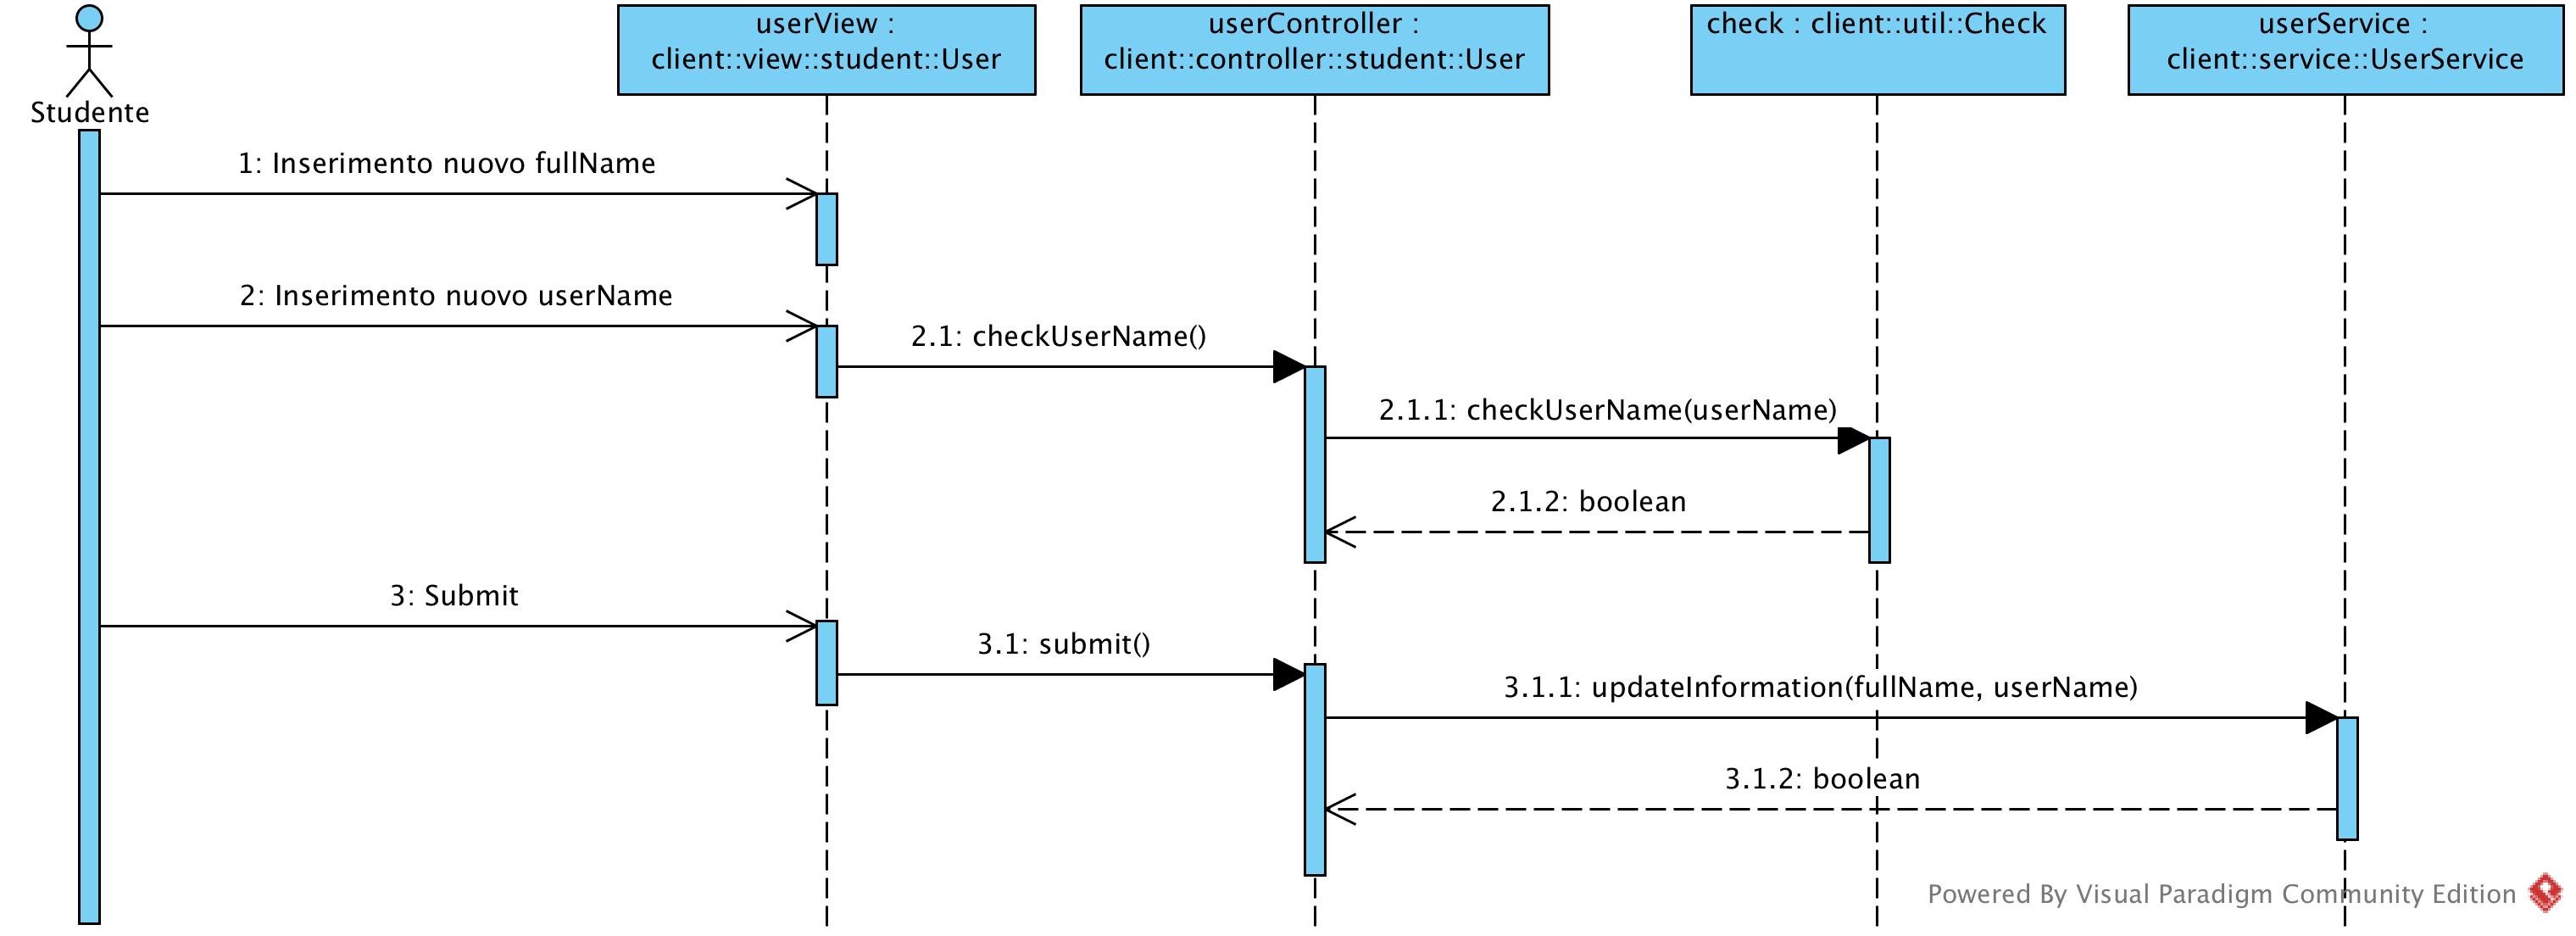
\includegraphics[max width=\myheight, angle=90]{../img/diagrammiSequenza/cambioInfoClient.png}
		\caption{Diagramma sequenza - Cambio Informazioni Client}
	\end{figure}
\end{center}

\newpage
\subsubsection{Cambio Password}
Di seguito viene presentato il diagramma di sequenza per il cambio della password da parte dell'utente connesso al sistema. L'utente inserisce la nuova password e la invia al controller il quale chiama i servizi adatti per modificare il profilo personale.Gli oggetti e attori attivi durante questa interazione sono:

\begin{itemize}
	\item \textbf{Studente:}  l'utente autenticato con ruolo di studente o superiore che ha intenzione di cambiare la password
	\item \textbf{userView:} è la pagina che mostra i dati dell'utente connesso al sistema
	\item \textbf{userController:} è il \mgls{controller} dell'applicazione che si occupa delle modifiche dell'utente, dal cambio di informazioni personali al cambio di password
	\item \textbf{userService:} è l'oggetto che si occupa di comunicare con il server per apportare le modifiche
\end{itemize}

\begin{center}
	\begin{figure}[H]
		\centering 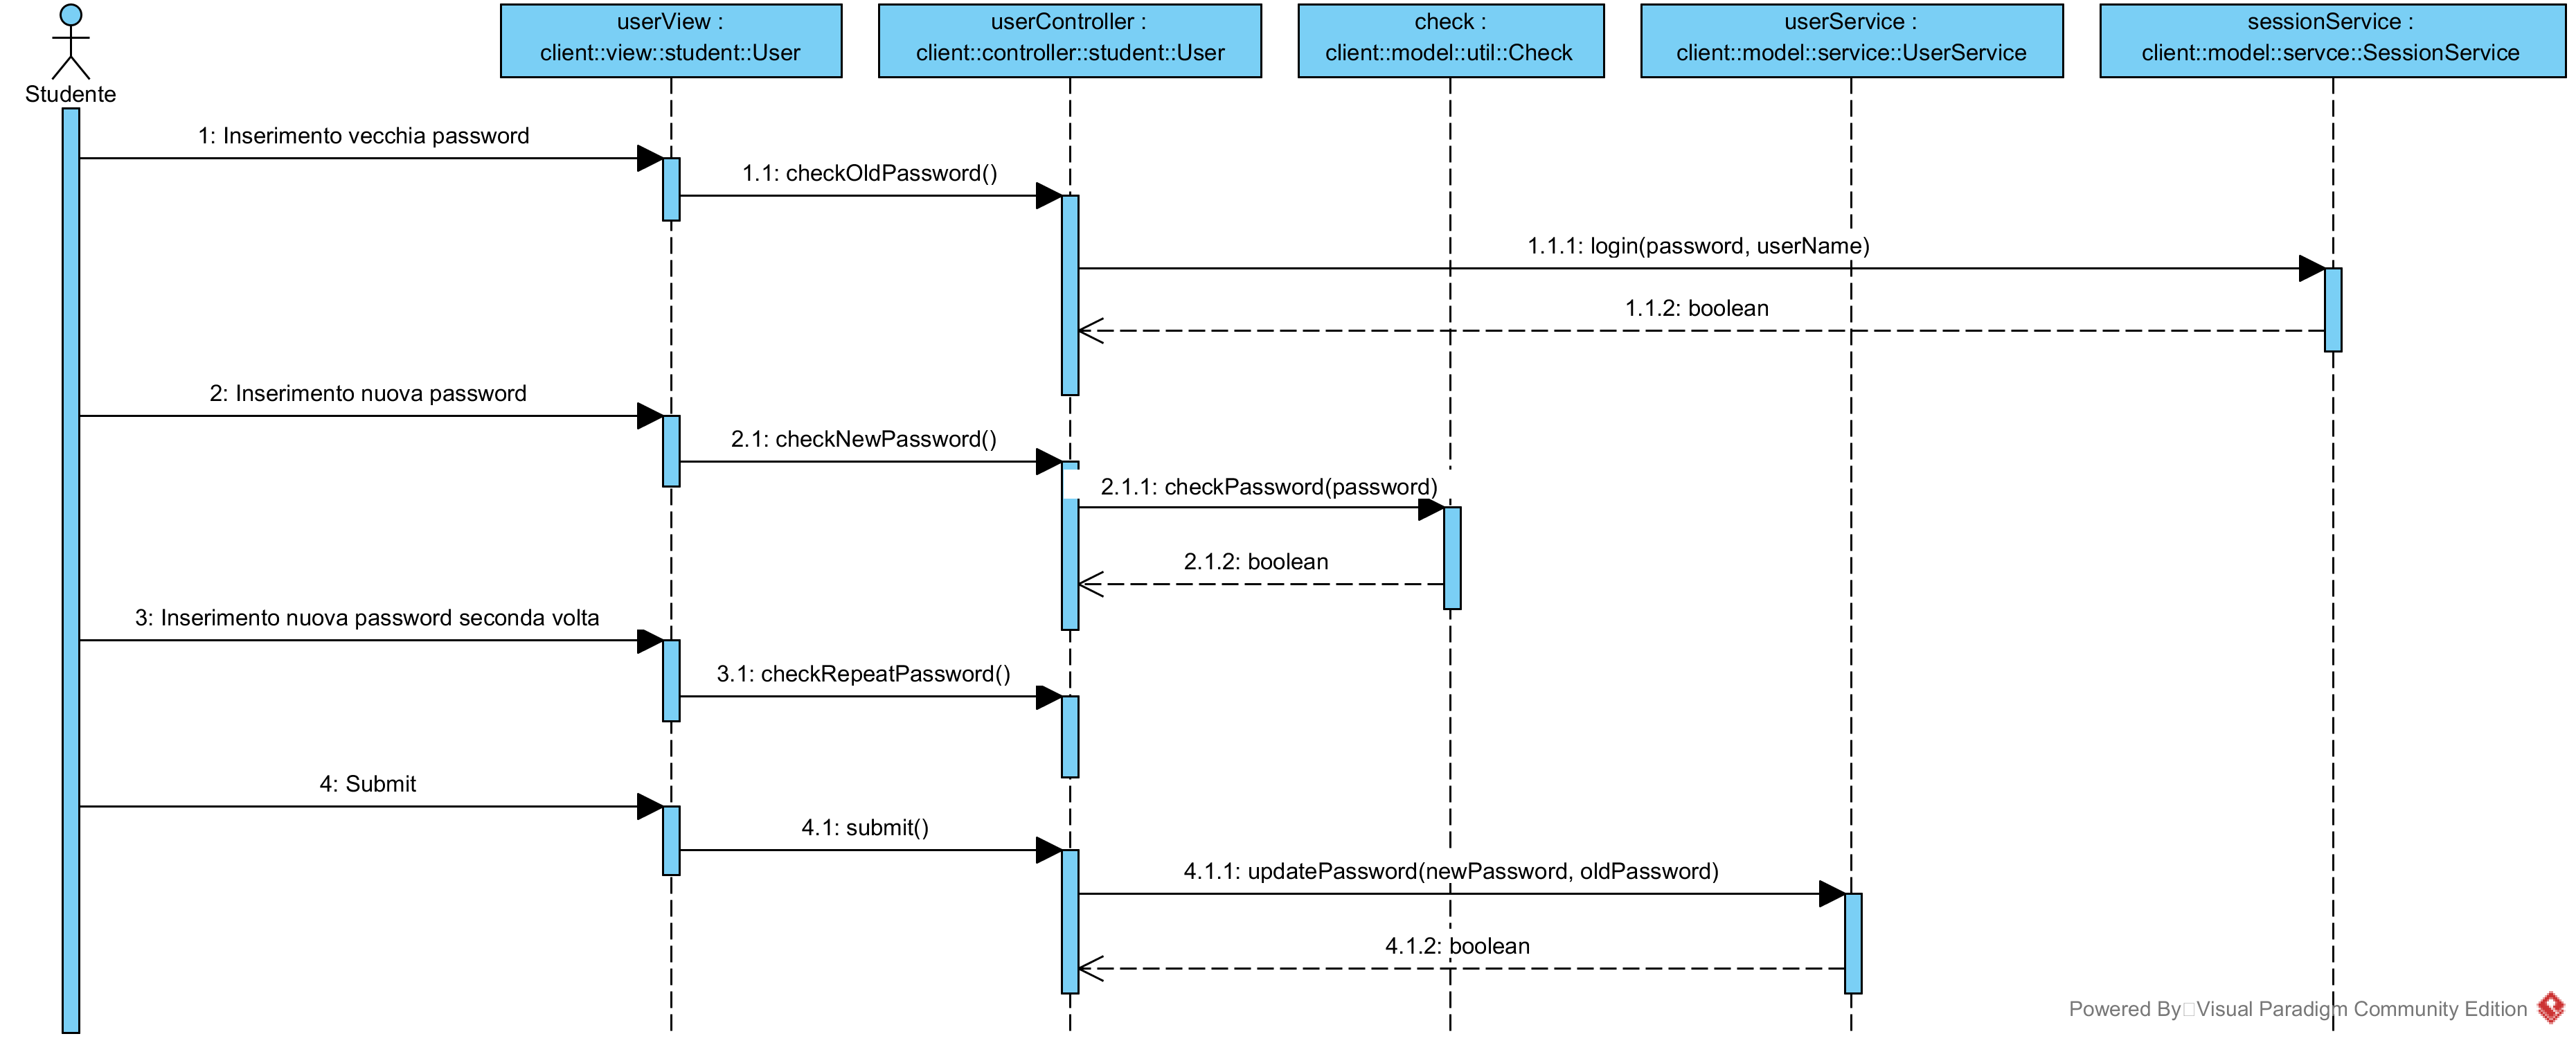
\includegraphics[max width=\myheight, angle=90]{../img/diagrammiSequenza/cambioPasswordClient.png}
		\caption{Diagramma sequenza - Cambio Password Client}
	\end{figure}
\end{center}

\newpage
\subsubsection{Inserisci Questionario}
Di seguito viene presentato il diagramma di sequenza per l'inserimento di un questionario da parte di un utente con ruolo docente o superiore. L'utente inserisce il titolo, gli argomenti e seleziona le domande da inserire, poi li passa al controller che chiama li servizio per aggiungere un questionario. Gli oggetti e attori attivi durante questa interazione sono:

\begin{itemize}
	\item \textbf{Docente:}	 l'utente autenticato con ruolo di docente o superiore che ha intenzione di inserire il questionario
	\item \textbf{manageQuestionnairesView:} è la pagina dell'applicazione che mostra la lista di tutti i questionari e permette la modifica o eliminazione di questionari esistenti o aggiunta di nuovi questionari
	\item \textbf{manageQuestionnairesController:} è il \mgls{controller} che permette di visualizzare e modificare i questionari della view corrispondente
	\item \textbf{manipulateQuestionnaireView:} rappresenta la pagina per la modifica o creazione di un singolo questionario
	\item \textbf{manipulateQuestionnaireController:} è il \mgls{controller} che si occupa di gestire le richieste dalla view corrispondente per la gestione o creazione di un singolo questionario
	\item \textbf{questionnaireService:} è l'oggetto che si occupa della comunicazione con il server per completare l'operazione di modifica o creazione del questionario
\end{itemize}

\begin{center}
	\begin{figure}[H]
		\centering 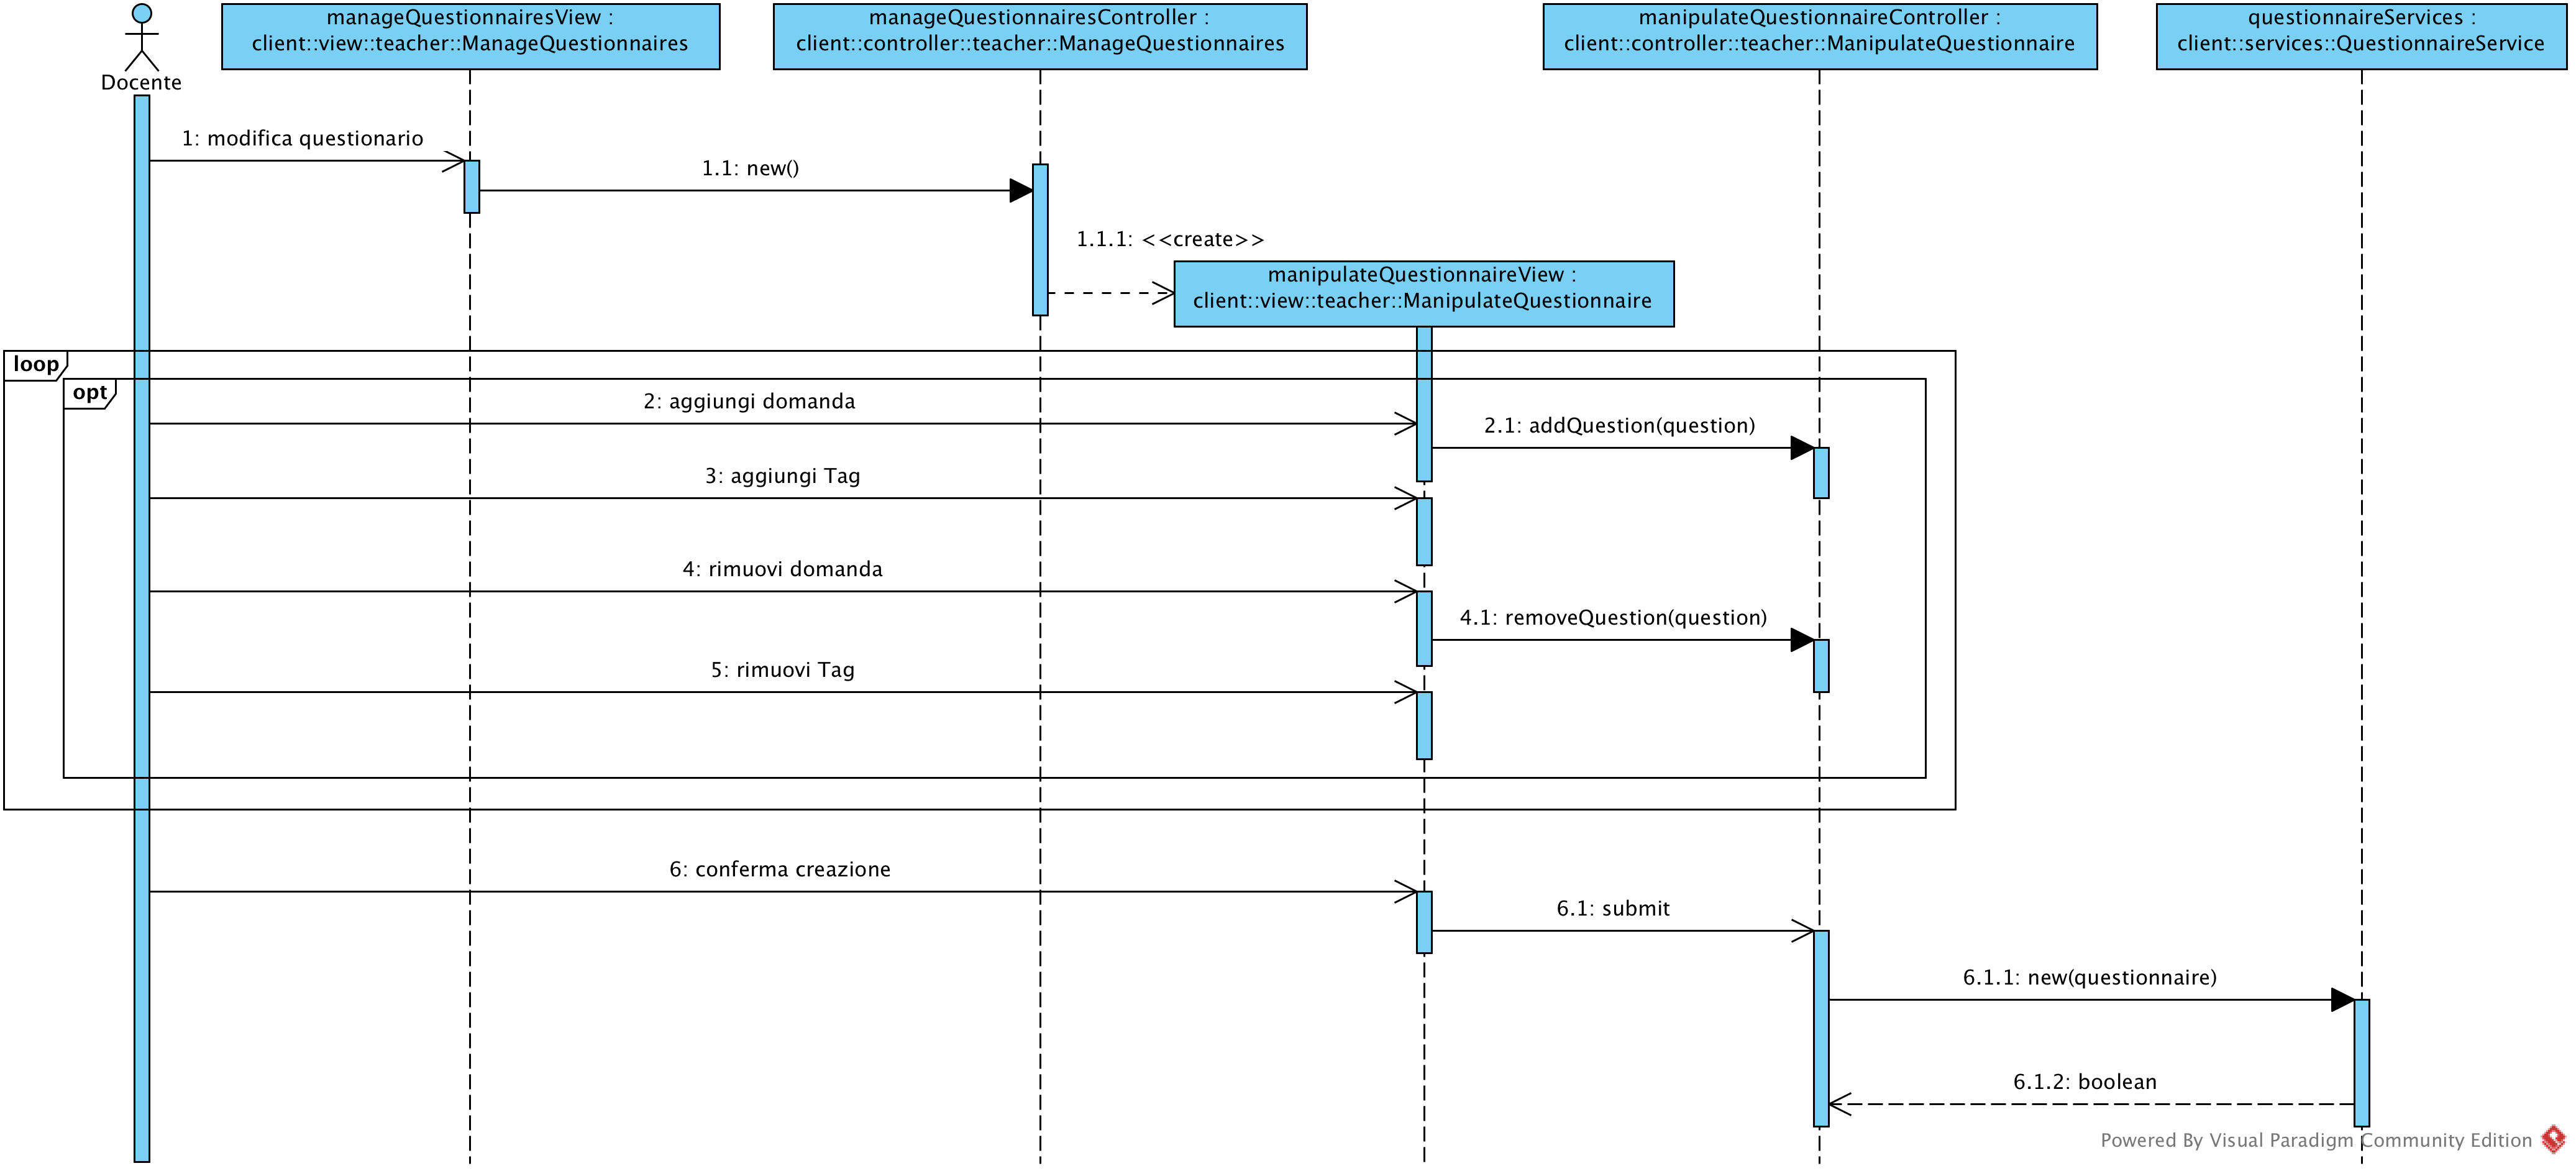
\includegraphics[max width=\myheight, angle=90]{../img/diagrammiSequenza/inserisciQuestionarioClient.png}
		\caption{Diagramma sequenza - Inserisci Questionario Client}
	\end{figure}
\end{center}

\newpage
\subsubsection{Esecuzione Questionario}
Di seguito viene presentato il diagramma di sequenza per l'inserimento di un questionario da parte di un utente con ruolo docente o superiore. Lo studente può rispondere alla domanda corrente, andare a quella precedente o quella successiva, poi, cliccando sulla funzionalità correggi, il controller chiama i servizi per verificare che tutte le domande abbiano una risposta e, in caso positivo, restituire il risultato del questionario. Gli oggetti e attori attivi durante questa interazione sono:

\begin{itemize}
	\item \textbf{Studente:}	 l'utente autenticato con ruolo di studente o superiore che ha intenzione di eseguire il questionario
	\item \textbf{executeQuestionnaireView:} rappresenta la pagina di visualizzazione del questionario in esecuzione
	\item \textbf{executeQuestionView:} rappresenta la pagina di visualizzazione di una singola domanda all'interno del questionario corrente
	\item \textbf{executeQuestionnaireController:} oggetto che gestisce la visualizzazione sequenziale delle domande da compilare per il questionario in esecuzione
	\item \textbf{executeQuestionController:} oggetto che gestisce la visualizzazione di una singola domanda all'interno del questionario in esecuzione
	\item \textbf{currentQuestionnaire:} oggetto che rappresenta i dati del questionario in esecuzione
\end{itemize}

\begin{center}
	\begin{figure}[H]
		\centering 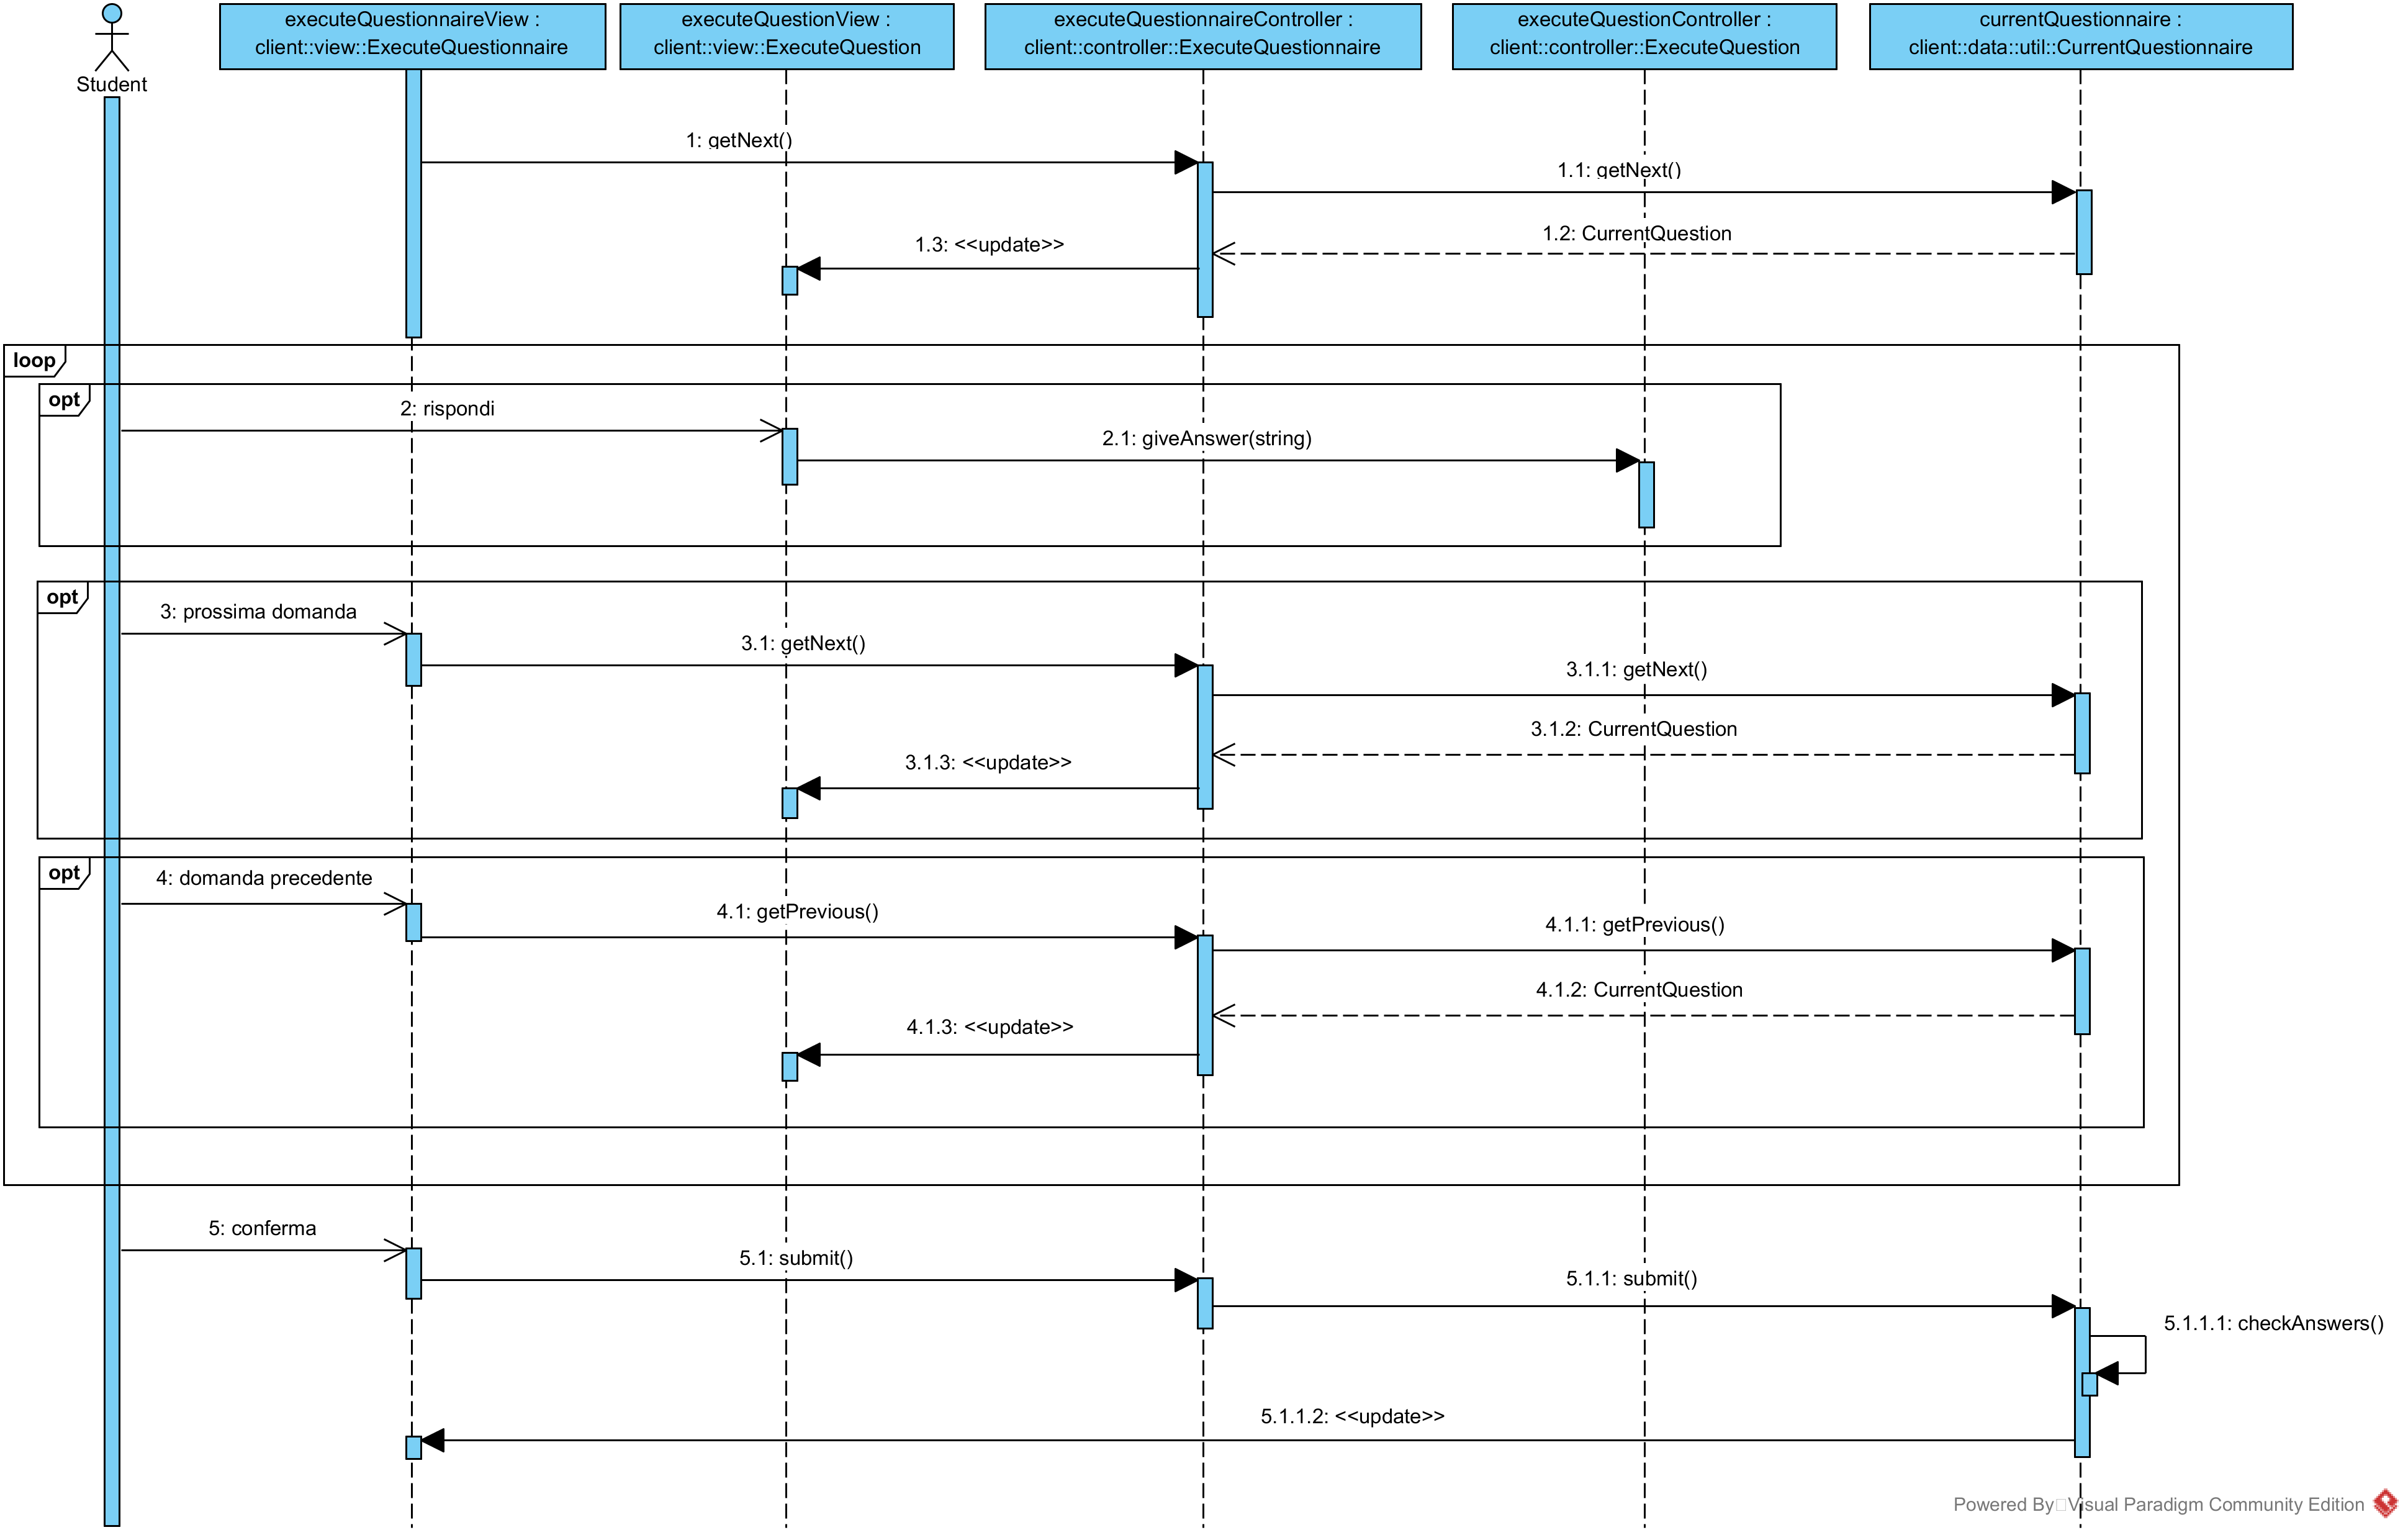
\includegraphics[max width=\myheight, angle=90]{../img/diagrammiSequenza/executeQuestionnaireClient.png}
		\caption{Diagramma sequenza - Esecuzione questionario Client}
	\end{figure}
\end{center}

\newpage
\subsubsection{Rimozione domanda}
Di seguito viene presentato il diagramma di sequenza del flusso per la rimozione di una domanda da parte del docente che la ha creata. L'utente seleziona la domanda da rimuovere e la rimuove, se questa non è presente in nessun questionario l'operazione va a buon fine, altrimenti viene visualizzato un messaggio di errore e la domanda non viene eliminata. Gli oggetti ed attori attivi durante questa operazione sono:

\begin{itemize}
	\item \textbf{router:} è l'oggetto che si occupa di smistare la richiesta in base all’URI ricevuto e ad invocare l’opportuno servizio
	\item \textbf{authorization:} è l'oggetto che si occupa di verificare i permessi dell'utente per ogni richiesta	
	\item \textbf{questionService:} è l'oggetto che si occupa di effettuare le modifiche nel database per l'aggiunta, rimozione e modifica di domande
	\item \textbf{errorHandler:} è il \mgls{middleware} che viene invocato verso la fine della richiesta che si occupa di trasformare eventuali errori nel formato \mgls{json} richiesto
\end{itemize}

\begin{center}
	\begin{figure}[H]
		\centering 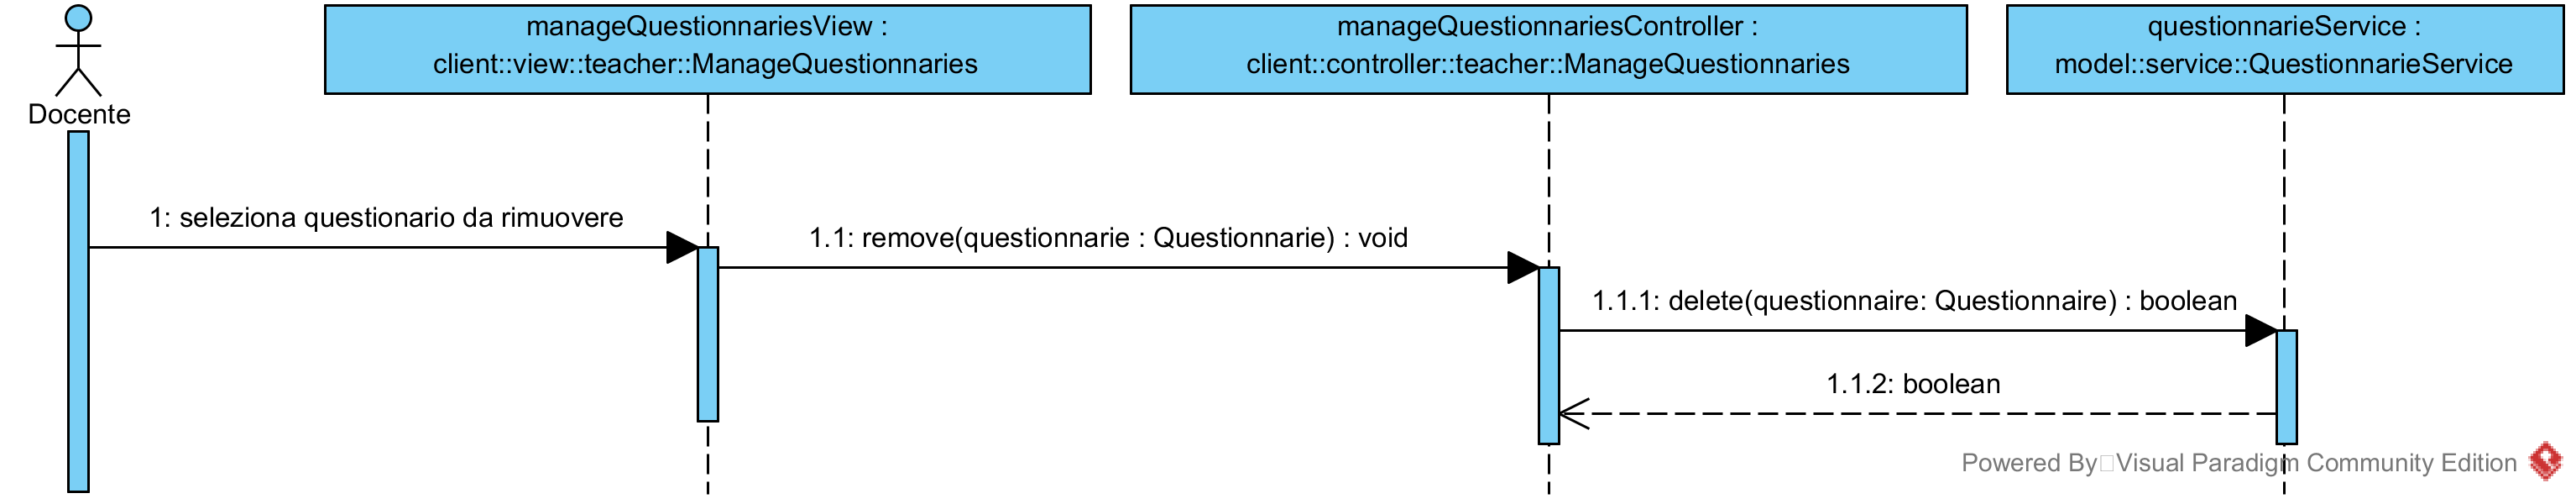
\includegraphics[max width=\myheight, angle=90]{../img/diagrammiSequenza/rimozioneQuestionarioClient.png}
		\caption{Diagramma sequenza - Rimozione domanda Server}
	\end{figure}
\end{center}

\newpage
\subsubsection{Modifica Questionario}
Di seguito viene presentato il diagramma di sequenza per la modifica di un singolo questionario da parte di un utente con ruolo di docente o superiore. Quando l'utente seleziona la funzionalità nella view, il controller semplicemente richiama il servizio per promuovere o degradare un certo utente. Gli oggetti e attori attivi durante questa interazione sono:

\begin{itemize}
	\item \textbf{Docente:}	 l'utente autenticato con ruolo di docente o superiore che ha intenzione di inserire il questionario
	\item \textbf{manageQuestionnairesView:} è la pagina dell'applicazione che mostra la lista di tutti i questionari e permette la modifica o eliminazione di questionari esistenti o aggiunta di nuovi questionari
	\item \textbf{manageQuestionnairesController:} è il \mgls{controller} che permette di visualizzare e modificare i questionari della view corrispondente
	\item \textbf{manipulateQuestionnaireView:} rappresenta la pagina per la modifica o creazione di un singolo questionario
	\item \textbf{manipulateQuestionnaireController:} è il \mgls{controller} che si occupa di gestire le richieste dalla view corrispondente per la gestione o creazione di un singolo questionario
	\item \textbf{questionnaireService:} è l'oggetto che si occupa della comunicazione con il server per completare l'operazione di modifica o creazione del questionario
\end{itemize}

\begin{center}
	\begin{figure}[H]
		\centering 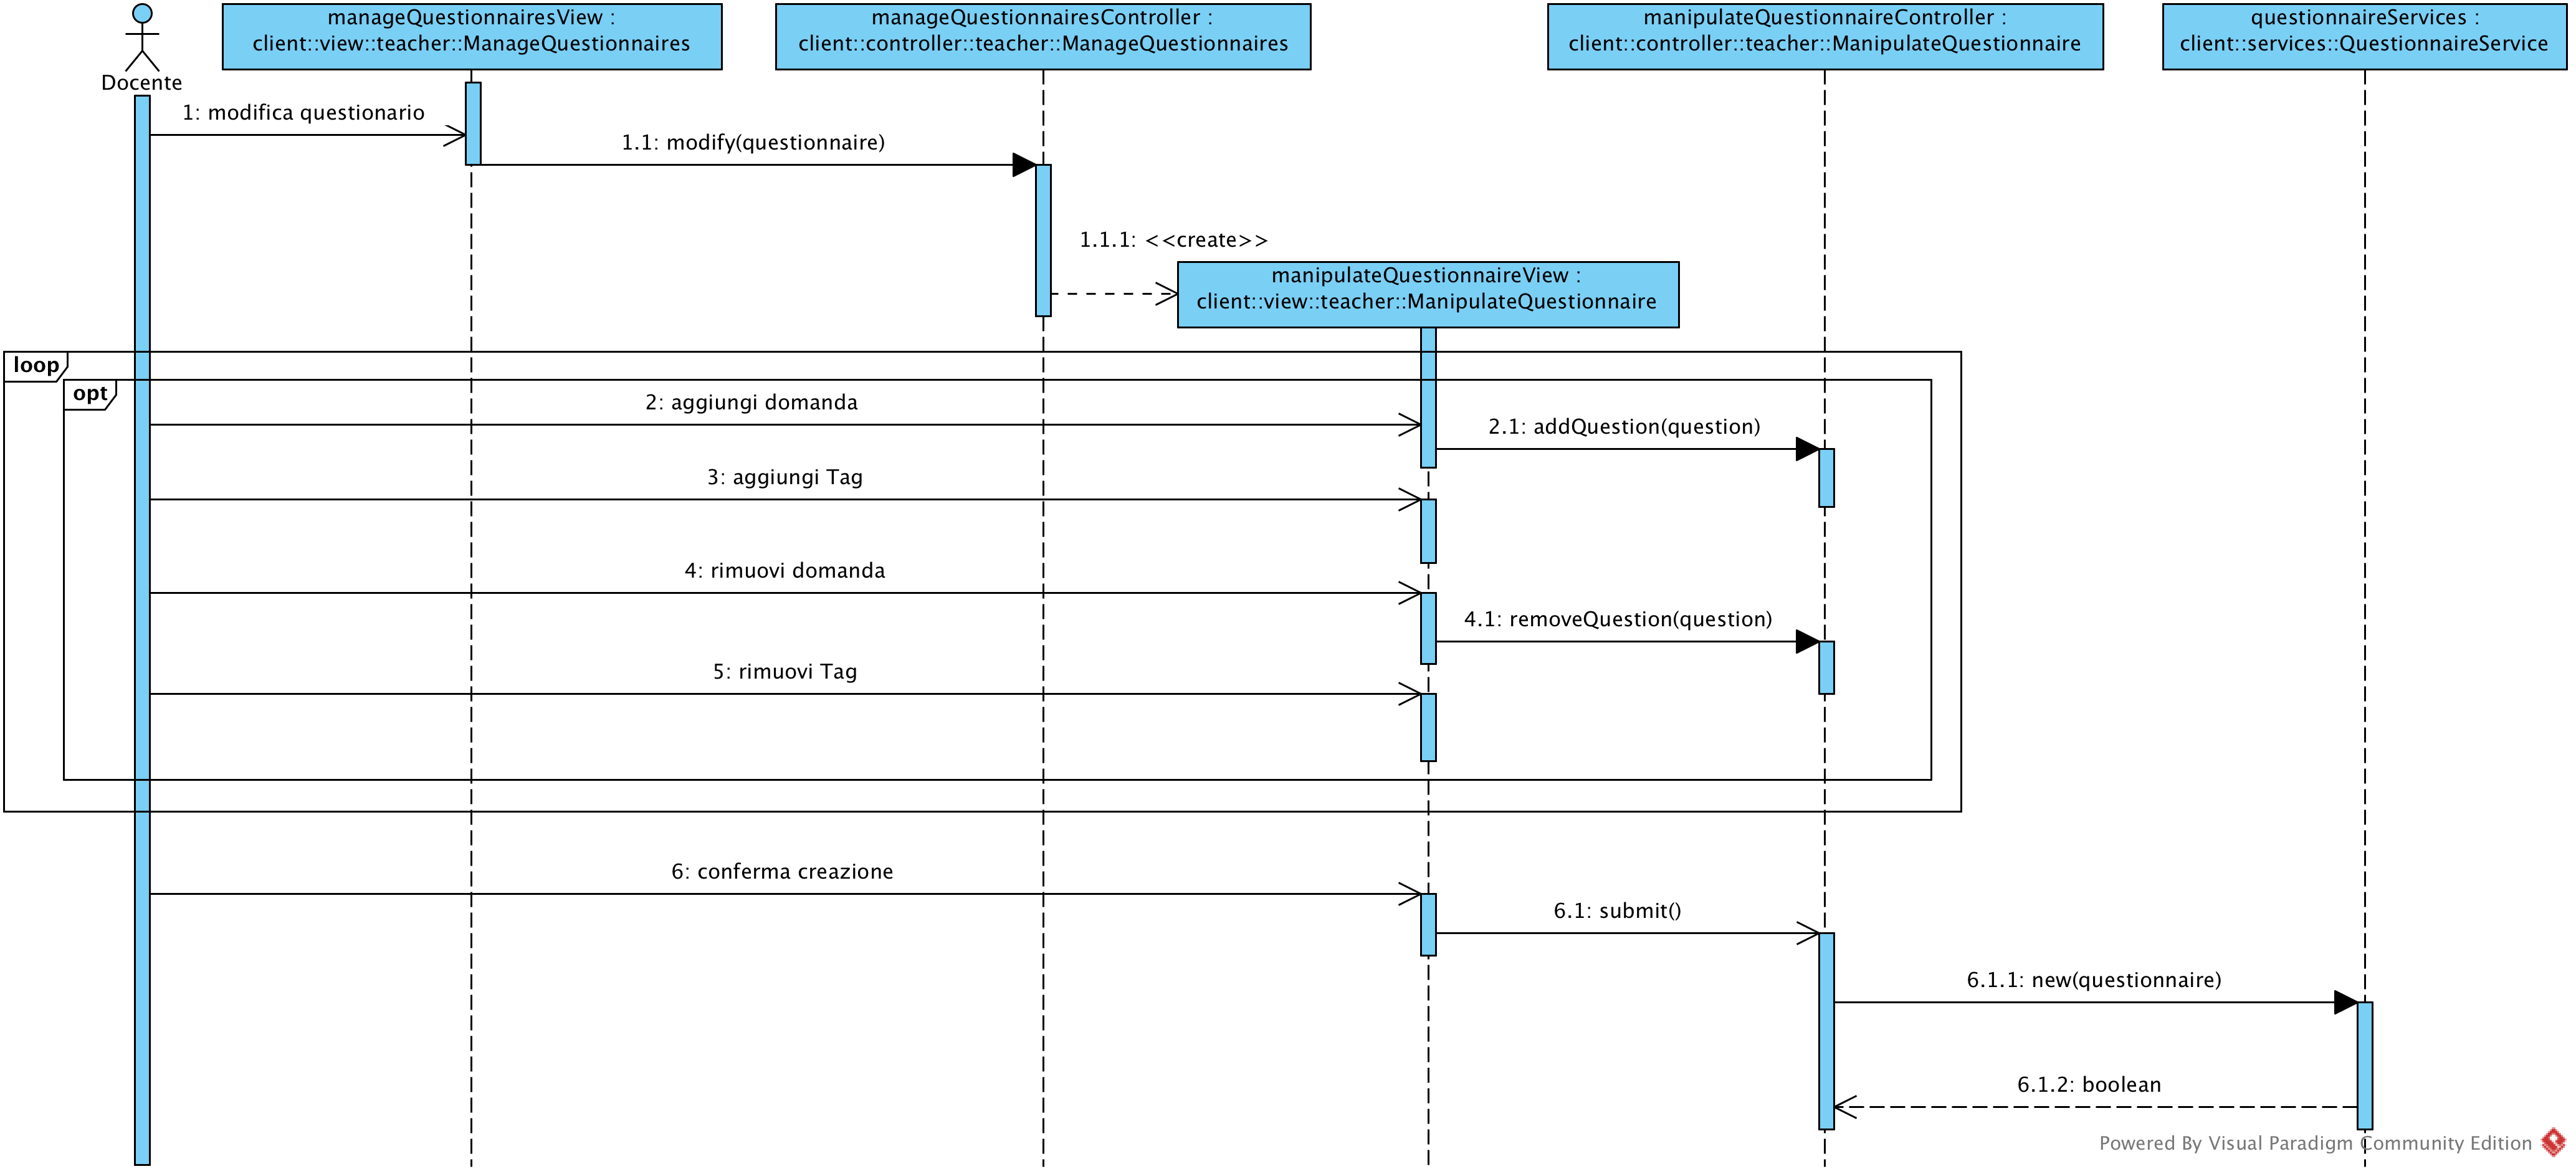
\includegraphics[max width=\myheight, angle=90]{../img/diagrammiSequenza/modificaQuestionarioClient.png}
		\caption{Diagramma sequenza - Modifica Questionario Client}
	\end{figure}
\end{center}

\newpage
\subsubsection{Rimozione Questionario}
Di seguito viene presentato il diagramma di sequenza per la rimozione di un questionario da parte di un docente. Il docente seleziona la domanda da rimuovere e il controller provvede a chiamare il servizio per effettuare l'operazione di rimozione attraverso la relativa API. Gli oggetti e attori attivi durante questa interazione sono:

\begin{itemize}
	\item \textbf{Docente:}	 l'utente autenticato con ruolo di docente o superiore che ha intenzione di inserire il questionario
	\item \textbf{manageQuestionnairesView:} è la pagina dell'applicazione che mostra la lista di tutti i questionari e permette la modifica o eliminazione di questionari esistenti o aggiunta di nuovi questionari
	\item \textbf{manageQuestionnairesController:} è il \mgls{controller} che permette di visualizzare, modificare o eliminare i questionari della view corrispondente
	\item \textbf{questionnaireService:} è l'oggetto che si occupa della comunicazione con il server per completare l'operazione di modifica, creazione o eliminazione del questionario
\end{itemize}

\begin{center}
	\begin{figure}[H]
		\centering 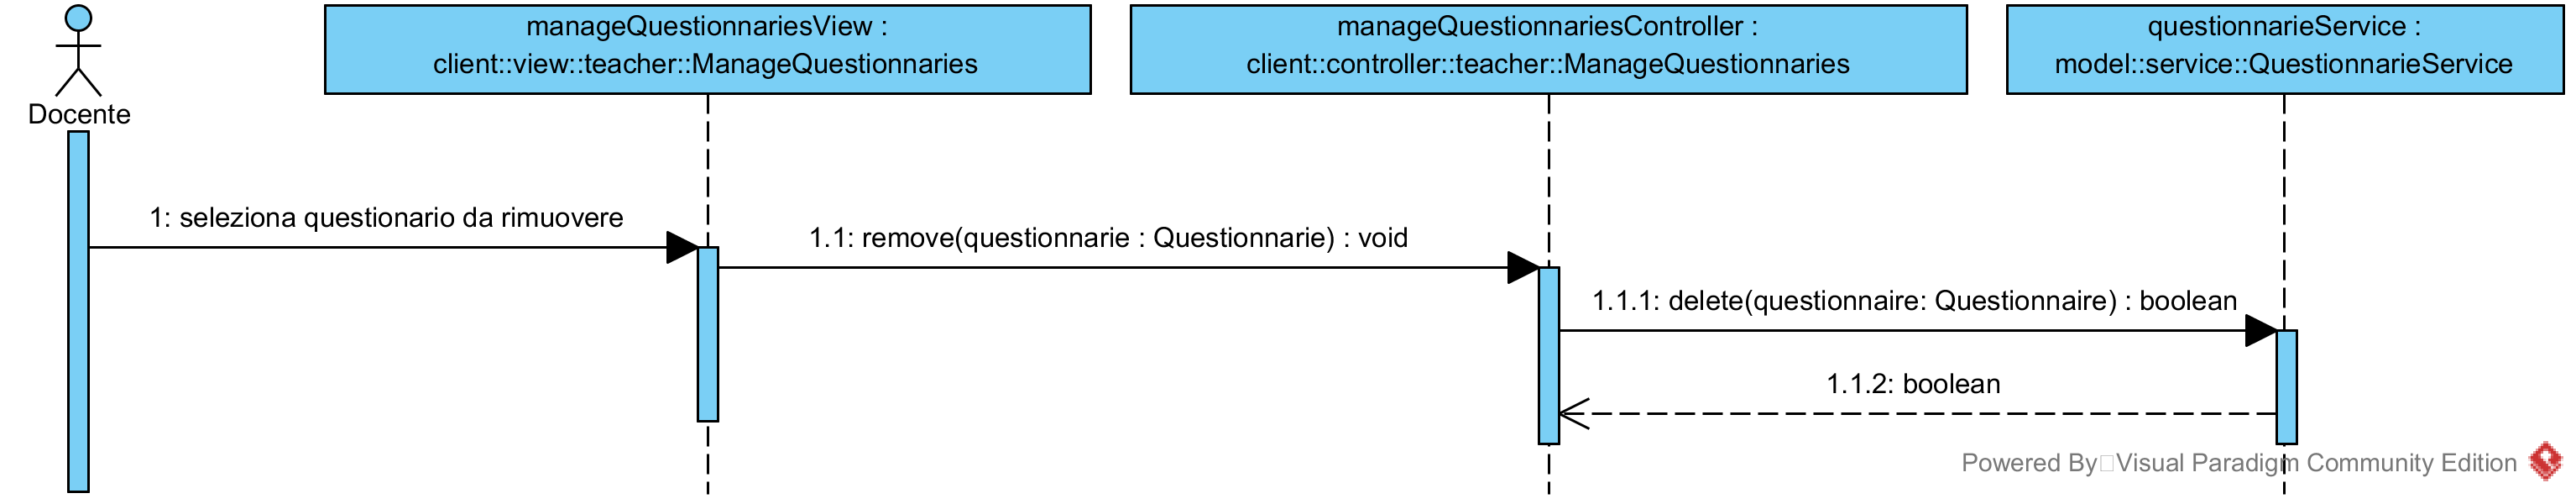
\includegraphics[max width=\myheight, angle=90]{../img/diagrammiSequenza/rimozioneQuestionarioClient.png}
		\caption{Diagramma sequenza - Rimozione Questionario Client}
	\end{figure}
\end{center}

\newpage
\appendix

\section{Descrizione Design Pattern}
\subsection{Design Pattern Architetturali}
\subsubsection{MVC}
Model-View-Controller (\mgls{mvc}) è un \mgls{design pattern} per l’implementazione di interfacce utente. Esso divide un’applicazione \mgls{software} in tre parti interconnesse, in modo da separare nettamente la rappresentazione interna dei dati dal modo in cui essa viene presentata all’utente. Il \mgls{model} è il modulo che contiene i dati. Una \mgls{view} può essere qualsiasi output dell’informazione, come ad esempio un testo o un diagramma. Si possono avere molteplici \mgls{view} della stessa informazione. La terza parte, il \mgls{controller}, si occupa di accettare degli input e di convertirli in comandi per il \mgls{model} o per la \mgls{view}.\\
Oltre a dividere l’applicazione in queste tre componenti, \mgls{mvc} si occupa anche di definire le interazioni tra esse:
\begin{itemize}
	\item Un \mgls{controller} gestisce gli input che vengono generati dalla \mgls{view} e può inviare comandi al \mgls{model} per aggiornare il suo stato. Inoltre seleziona quale view deve essere eseguita e visualizzata;
	\item Un \mgls{model} quando cambia il suo stato interno notifica le \mgls{view} associate. Questo permette alle \mgls{view} di cambiare la loro presentazione;
	\item Una \mgls{view} riceve aggiornamenti dal \mgls{model} per cambiare il suo stato e notifica al \mgls{controller} i comandi dell'utente.
\end{itemize}

\begin{center}
	\begin{figure}[H]
		\centering 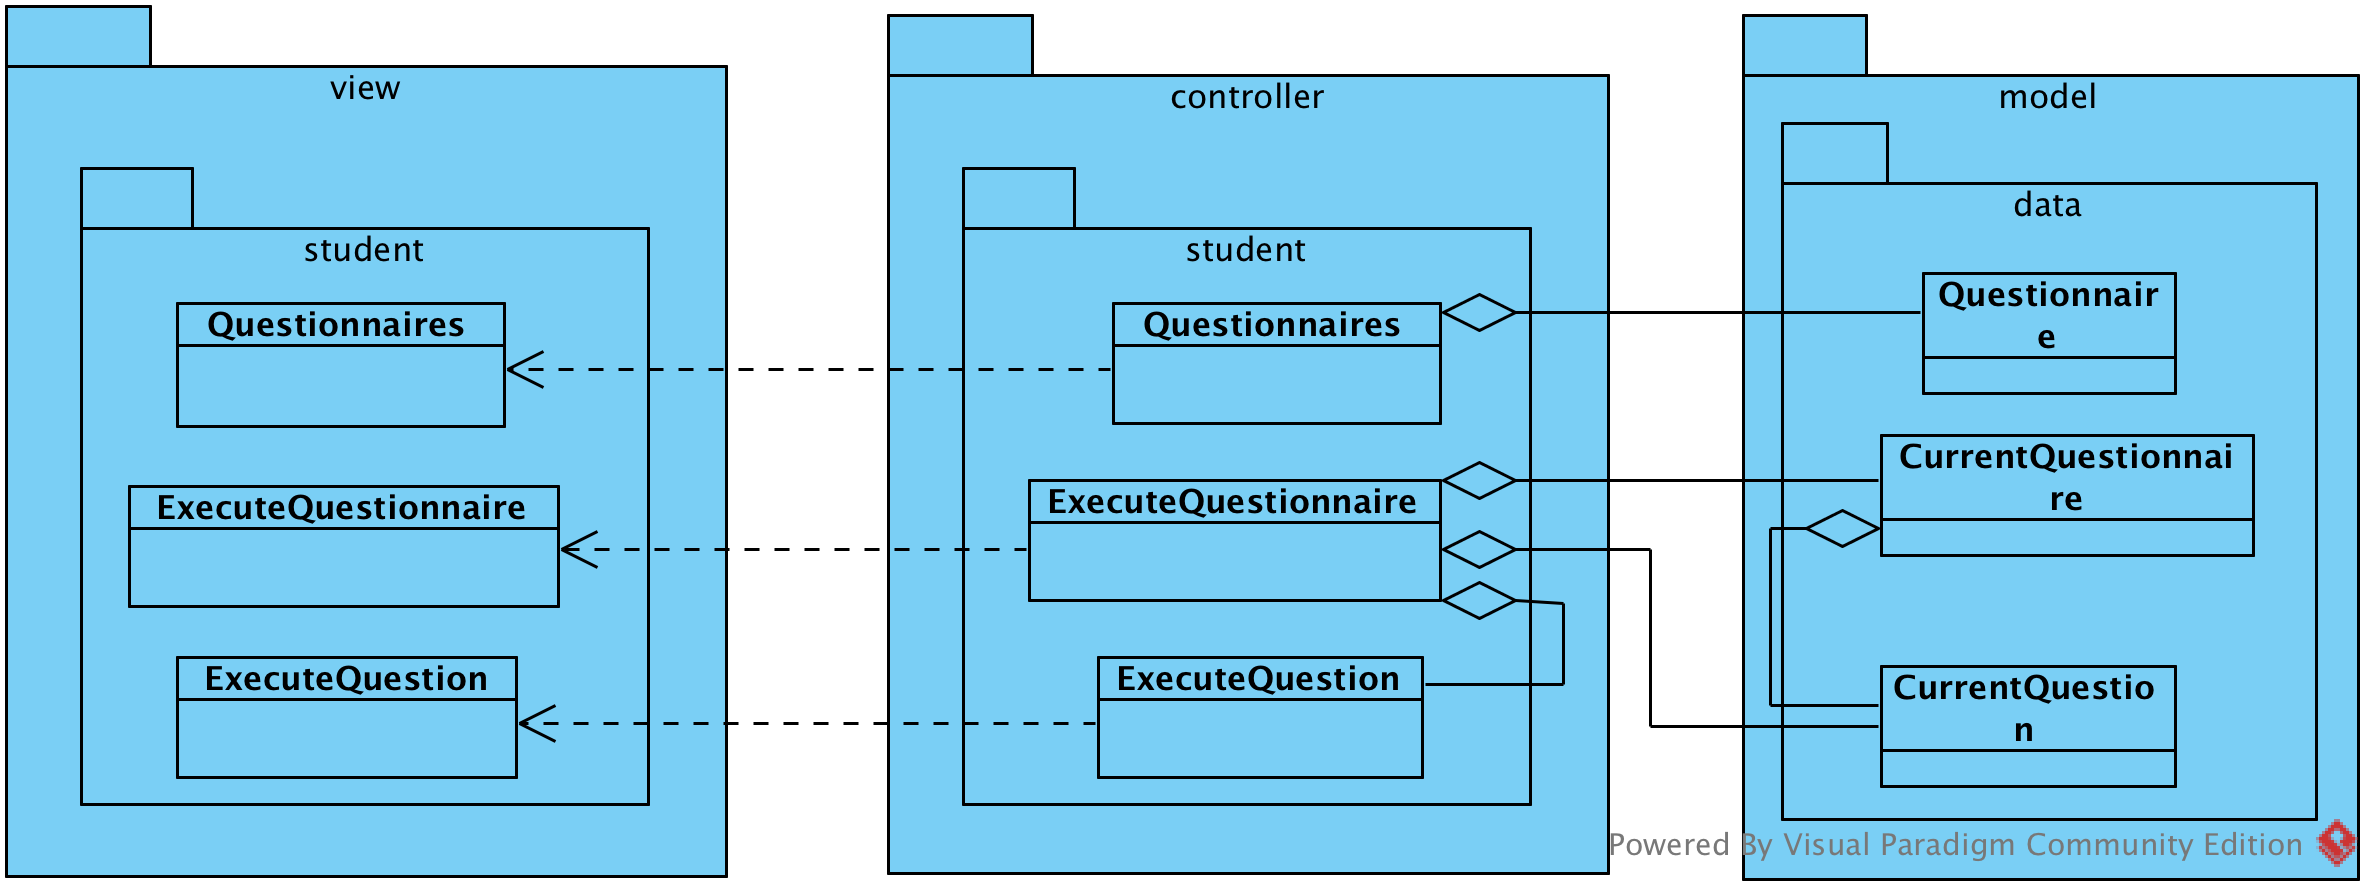
\includegraphics[max width=\textwidth]{../img/mvcStarware.png}
		\caption{Esempio dell' applicazione di MVC in Quizzipedia}
	\end{figure}
\end{center}

Sebbene inizialmente sviluppata per applicazioni \mgls{desktop}, \mgls{mvc} è stato usato moltissimo come architettura per le Web application in tutti i principali linguaggi di programmazione. Moltissimi \mgls{framework} commerciali e non sono stati progettati utilizzando questo \mgls{design pattern}.

\subsubsection{Middleware}
Il Middleware è uno strato \mgls{software} che si interpone tra l’applicazione \mgls{software} e uno strato di servizi per semplificarne le comunicazioni e la gestione di input/output. Viene solitamente utilizzato in applicazioni distribuite e facilita l’interoperabilità, fornendo servizi che permettono la comunicazione tra applicazioni di sistemi operativi diversi. Può accedere che il Middleware fornisca dei servizi abitualmente attribuibili a un sistema operativo. I servizi Middleware forniscono un set di interfacce che permetto a un’applicazione di:
\begin{itemize}
	\item Localizzare facilmente applicazioni o servizi in una rete;
	\item Filtrare dati per renderli user-friendly oppure anonimizzarli per renderli pubblicabili, proteggendone la privacy;
	\item Essere indipendente dai servizi di rete;
	\item Essere affidabile e sempre disponibile;
	\item Aggiungere attributi complementari.
\end{itemize}
Si tratta quindi di funzionalità leggermente più specializzate da quelle normalmente offerte da un sistema operativo. L’avvento del web ha avuto una forte ripercussione sulla diffusione dei \mgls{software} di Middleware. Essi hanno infatti permesso l’accesso sicuro da remoto a \mgls{database} locali. I tipi di Middleware sono:
\begin{itemize}
	\item \textbf{Message-Oriented Middleware (MOM):} sono Middleware dove le notifiche degli	eventi vengono spedite come messaggi tra sistemi o componenti. I messaggi inviati al
	\mgls{client} vengono memorizzati fintanto che non vengono gestiti, nel frattempo il \mgls{client} può	svolgere altro lavoro 
	\item \textbf{Enterprise messaging system:} è un tipo di Middleware che facilita il passaggio di messaggi tra sistemi diversi o componenti in formato standard, spesso utilizzando servizi web o \mgls{xml}
	\item \textbf{Message broker:} è parte dell'entreprise messaging system. Accoda, duplica, traduce e spedisce messaggi a sistemi o componenti diverse
	\item \textbf{Enterprise Service Bus:} è definito come qualche tipo di Middleware integrato che supporta sia MOM che dei servizi web
	\item \textbf{Intelligent Middleware:} gestisce il processamento in tempo reale di grandi volumi di segnali che trasforma in informazioni di business. Particolarmente adatto per architetture scalabili e distribuite
	\item \textbf{Content-Centric Middleware:} questo tipo di Middleware fornisce una semplice astrazione con la quale le applicazioni possono inoltrare richieste per contenuti univocamente identificati, senza occuparsi su come e dove vanno ottenuti
\end{itemize}

\subsection{Design Pattern Creazionali}
\subsubsection{Singleton}
Il Singleton è un \mgls{design pattern} creazionale che permette di avere un’unica istanza di una classe con un unico punto di accesso noto. Tale condizione è tipica di alcuni contesti e trova risvolti pratici in svariate applicazioni. Per permettere l’implementazione di questo pattern è sufficiente che la classe stessa si occupi di tracciare la propria istanziazione e bloccarla qualora sia già avvenuta almeno una volta. Il Singleton dovrebbe essere estensibile usando il \mgls{subclassing}. Il \mgls{client} può utilizzarne l’estensione senza quindi modificarne il codice.\\
L’utilizzo di questo \mgls{design pattern} comporta una serie di conseguenze:
\begin{itemize}
	\item accesso controllato alla singola istanza: poiché la classe Singleton incapsula la sua unica istanza, è in grado di controllare quando e come i \mgls{client} vi accedono;
	\item \mgls{namespace} pulito: l’utilizzo di questo pattern risulta migliore rispetto all’uso di variabili globali poiché scongiura l’inquinamento del \mgls{namespace} globale;
	\item permette raffinamenti di operazioni e rappresentazioni: il Singleton dovrebbe venire sempre esteso prima dell’utilizzo, che in termini pratici si traduce in un operazione banale. Questo può avvenire anche a runtime;
	\item eventualmente permette un numero variabile di istanze: questo pattern permette, se necessario, di avere istanze multiple mantenendo però il controllo sul numero;
	\item flessibilità: un modo per avere una funzionalità riconducibile al Singleton è quello di utilizzare le operazioni sulle classi, come per esempio la keyword static del C++, ma in questo modo è più difficile controllarne il design e permetterne più istanze. Inoltre nel linguaggio succitato le funzioni statiche non sono mai virtuali, rendendone impossibile l’utilizzo polimorfo alle sottoclassi che le ridefinisco.
\end{itemize}

%Non utilizzato per ora
%\subsubsection{Registry}
%Il Registry è simile ad un oggetto globale che gli altri oggetti usano per accedere a servizi e oggetti comuni. Quando si vuole recuperare un oggetto capita spesso di accedervi tramite un altro oggetto legato da un qualche tipo di associazione, ma in alcuni casi non è possibile conoscere a priori l’oggetto da cui partire, così vi è la necessità di avere un metodo di look-up accedibile tramite il Registry. Le interfacce del Registry possono essere metodi statici.

%Non utilizzato per ora
%\subsubsection{Factory method}
%Questo pattern definisce un’interfaccia per la creazione di un oggetto, lasciando alle sottoclassi la decisione sulla classe che deve essere istanziata. Consente inoltre di deferire l’istanziazione di una classe alle sottoclassi. Tra i suoi utilizzi ci sono i seguenti casi:
%\begin{itemize}
	%\item Quando una classe non è in grado di sapere in anticipo le classi degli oggetti che deve creare;
	%\item Quando una classe vuole che le sue sottoclassi scelgano gli oggetti da creare;
	%\item Quando le classi delegano la responsabilità a una o più classi di supporto e si vuole localizzare in un punto ben preciso la conoscenza di quale o quali classi di supporto vengano delegate.
%\end{itemize}

\subsection{Design Pattern Strutturali}
\subsubsection{Facade}
Questo pattern fornisce un’interfaccia unificata per un insieme di interfacce presenti in un sottosistema. Facade definisce un’interfaccia di alto livello che rende il sottosistema più semplice da utilizzare. Suddividere un sistema in sottosistemi aiuta a ridurne la complessità. Può essere utilizzato nei seguenti casi:
\begin{itemize}
	\item Quando si vuole fornire un’interfaccia semplice a un sottosistema complesso. La complessità dei sottosistemi tende ad aumentare con la loro evoluzione. Molti pattern, quando applicati, portano a un aumento nel numero di classi piccole. Ciò rende il sottosistema maggiormente riusabile e semplice da personalizzare, ma di utilizzo più difficile per i \mgls{client} che non richiedono alcuna personalizzazione. Un Facade può fornire una vista semplice di base su un sottosistema che si rivela essere sufficiente per la maggior parte dei \mgls{client}. Soltanto i \mgls{client} che richiedono una personalizzazione maggiore dovranno guardare dietro la facciata;
	\item Nei casi in cui sono molte le dipendenze fra i \mgls{client} e le classi che implementano un’astrazione. Introducendo un Facade si disaccoppia il sottosistema dai \mgls{client} e dagli altri sottosistemi, promuovendo quindi la portabilità e l’indipendenza di sottosistemi;
	\item Quando si vogliono organizzare i sottosistemi in una struttura a livelli. Un Facade può essere utilizzato per definire un punto di ingresso ad ogni livello. Nel caso in cui i sottosistemi non siano indipendenti e le dipendenze esistenti possano essere semplificate facendo comunicare tra loro i sottosistemi soltanto attraverso i rispettivi oggetti Facade.
\end{itemize}

\begin{center}
	\begin{figure}[H]
		\centering 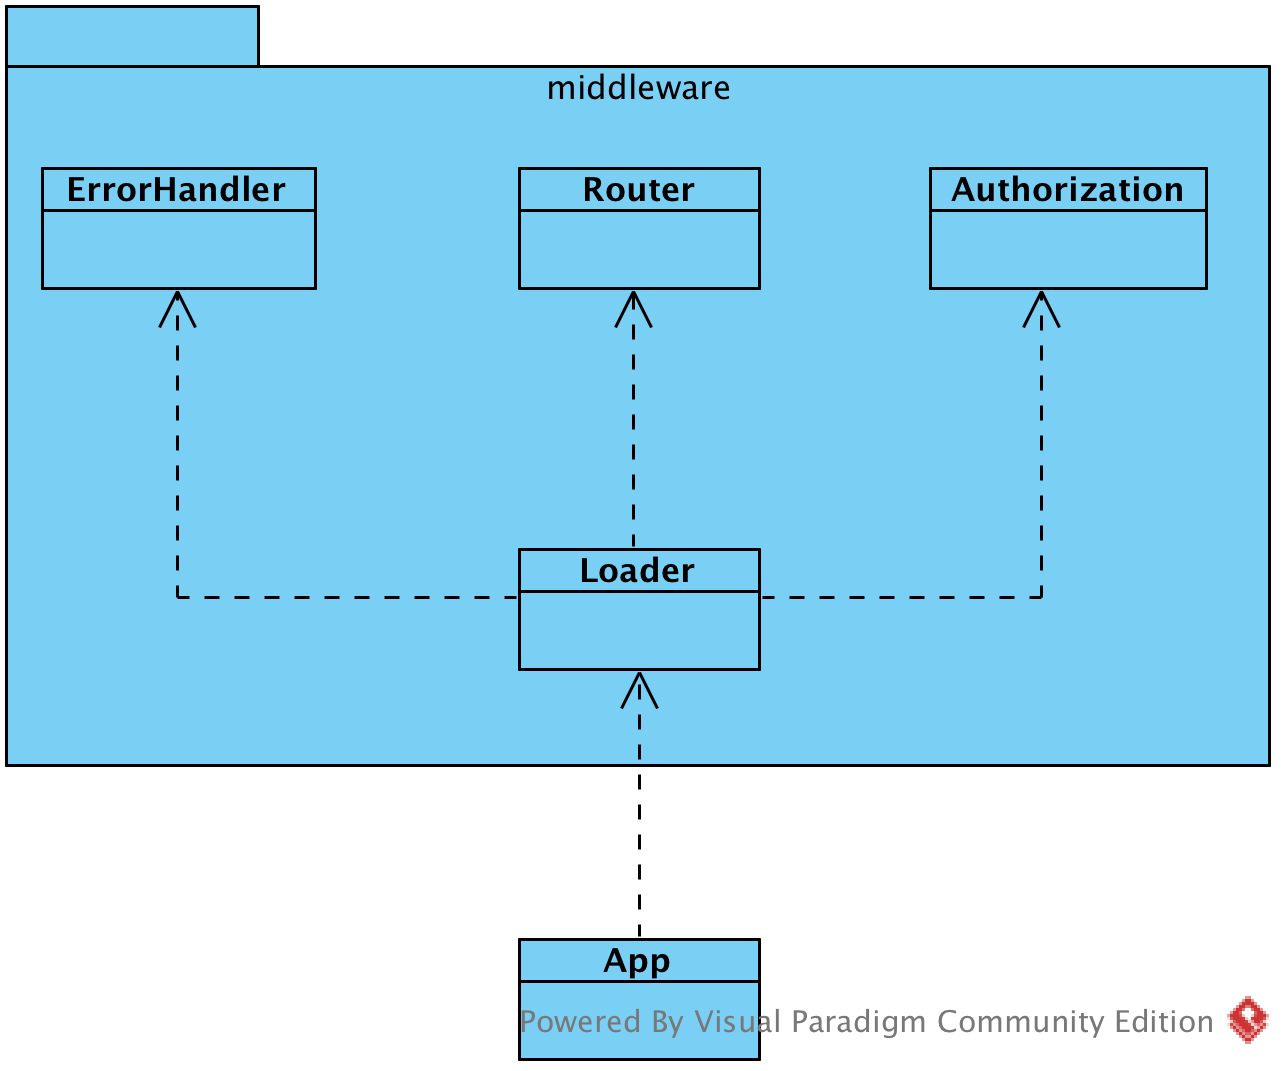
\includegraphics[max width=\textwidth]{../img/facadeStarware.png}
		\caption{Esempio dell' applicazione del pattern Facade in Quizzipedia}
	\end{figure}
\end{center}

\subsection{Design Pattern Comportamentali}
\subsubsection{Chain of Responsibility}
Il Chain of Responsibility è un pattern comportamentale che permette di separare i \mgls{sender} dai \mgls{receiver} delle richieste. La richiesta attraversa una catena di oggetti per essere intercettata solo quando raggiunge il proprio gestore. Viene utilizzato quando non è possibile determinare staticamente il \mgls{receiver} oppure l’insieme di oggetti gestori cambia dinamicamente a runtime. Le richieste vengono dette implicite poiché il \mgls{sender} non ha alcuna conoscenza sull’identità del ricevente. Per permettere alla richiesta di attraversare la catena e per rimanere implicita, ogni \mgls{receiver} condivide un interfaccia comune per gestire le richieste ed accedere al proprio successore. La gerarchia che vorrà inviare richieste dovrà avere una superclasse che dichiara un metodo handler generico. La specializzazione di tale metodo avviene tramite overriding nelle sottoclassi opportune.\\
L’utilizzo di questo pattern comporta una serie di conseguenze:
\begin{itemize}
	\item Ridotto accoppiamento: gli oggetti non sono a conoscenza di chi gestirà la richiesta ma sanno solo che verrà gestita in modo appropriato. Inoltre non bisognerà manutenere i riferimenti a tutti i possibili riceventi;
	\item Aggiunge flessibilità nell’assegnamento delle responsabilità degli oggetti: è possible distribuire le responsabilità tra gli oggetti a runtime modificandone la gerarchia. Staticamente è possibile usare il |\mgls{subclassing} per specializzare i gestori;
	\item Non c’è garanzia che la richiesta venga gestita, questo può avvenire quando la catena non è stata costruita in modo rigoroso.
\end{itemize}

\begin{center}
	\begin{figure}[H]
		\centering 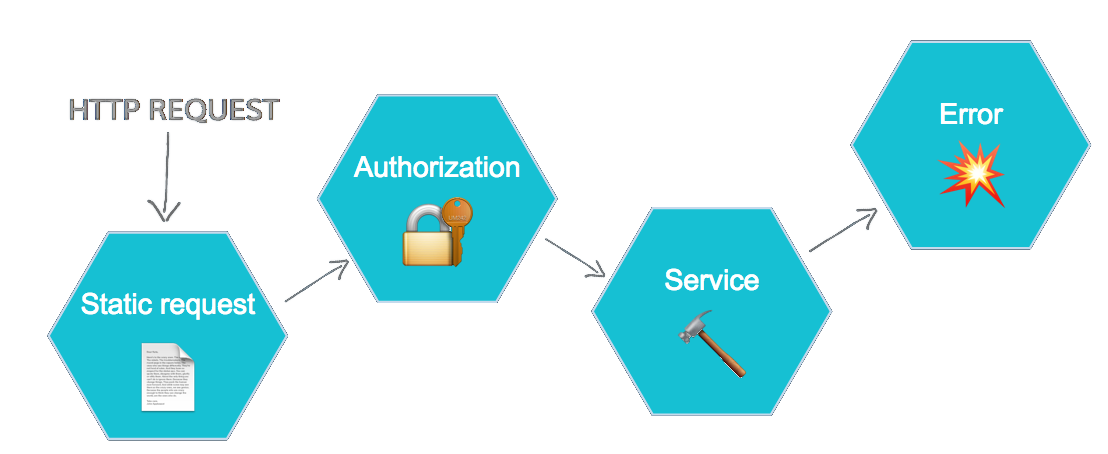
\includegraphics[max width=\textwidth]{../img/corStarware.png}
		\caption{Funzionamento del Chain of responsibility in Quizzipedia}
	\end{figure}
\end{center}

%Non utilizzato per ora
%\subsubsection{Strategy}
%Strategy ha come scopo quello di definire una famiglia di algoritmi, incapsularli e renderli intercambiabili. Permette agli algoritmi di variare indipendentemente dal client che ne fa uso. È opportuno usare il pattern strategy nei seguenti casi:
%\begin{itemize}
	%\item Molte classi correlate differiscono fra loro solo per il comportamento. Strategy fornisce un modo per configurare una classe con un comportamento scelto fra tanti;
	%\item Sono necessarie più varianti di un algoritmo. Per esempio, è possibile definire più algoritmi con bilanciamenti diversi fra occupazione in memoria, velocità di esecuzione, ecc. Possiamo usare il pattern Strategy quando queste varianti sono implementate sotto forma di gerarchia di classi di algoritmi;
	%\item Un algoritmo usa una struttura dati che non dovrebbe essere resa nota ai client. Il pattern strategy può essere usato per evitare di esporre strutture dati complesse e specifiche dell’algoritmo;
	%\item Una classe definisce molti comportamenti che compaiono all’interno di scelte condizionali multiple. Al posto di molte scelte condizionali si suggerisce di spostare i blocchi di codice correlati in una classe Strategy dedicata.
%\end{itemize}

%Non utilizzato per ora
%\subsubsection{Dependency Injection}
%Il Dependency Injection è un Design Pattern che permette la separazione del comportamento degli oggetti dalla loro dipendenze. Invece di istanziare le classi in modo diretto ogni componente riceve i riferimenti agli altri componenti necessari come parametri nel costruttore. Un utilizzo comune è quello con i plugin che vengono caricati dinamicamente. Gli elementi coinvolti sono:
%\begin{itemize}
	%\item Un dipendente consumatore;
	%\item Una dichiarazione delle dipendenze tra la componenti, definita come contratto di un interfaccia;
	%\item Un injector che crea istanze di classi che implementano una data dipendenza su richiesta.
%\end{itemize}
%Il dependent object dichiara da quali componenti dipende. L’injector decide quali classi soddisfano suoi requisiti e in caso affermativo gliele fornisce. Questa operazione può avvenire anche a runtime. Questo è un chiaro vantaggio poiché possono essere create dinamicamente diverse implementazioni di un componente software da passare allo stesso test. In questo modo il test può testare componenti diverse senza sapere che le loro implementazioni sono diverse. Lo scopo principale di questo pattern è quello di permettere una selezione a runtime su più implementazioni di una interfaccia dipendente. È particolarmente utile per fornire delle implementazioni di stub per componenti complesse, ma anche per gestire i plugin e per inizializzare servizi software. I test di unità comportano delle problematiche, poiché spesso richiedono la presenza di una parte di infrastruttura non ancora implementata. Il Dependency Injection semplifica il processo di testing per un istanza isolata. Poiché le componenti dichiarano le proprie dipendenze, un test può automaticamente istanziare le componenti necessarie.\\
%L’utilizzo di questo pattern comporta una serie di conseguenze:
%\begin{itemize}
	%\item Vi è una riduzione di Boilerplate code poiché il lavoro di set up delle dipendenze viene gestito da un componente dedicato;
	%\item Offre una certa flessibilità di configurazione perché diverse implementazione di un servizio posso essere usate senza essere ricompilate;
	%\item Facilita la scrittura di codice testabile;
	%\item Le dipendenze dichiarate sono black box, questo rende più difficile trovare gli errori al loro interno;
	%\item Le dipendenze non completamente implementate o errate generano errori a runtime e non a tempo di compilazione;
	%\item Rende il codice più difficile da manutenere;
	%\item L’injection a runtime di dipendenze va ad inficiare le prestazioni;
	%\item I benefici sono difficilmente commisurabili rispetto ai costi di implementazione.
%\end{itemize}
%Di seguito vengono elencati tre modi con cui un oggetto può ricevere un riferimento da un modulo esterno:
%\begin{itemize}
	%\item \textbf{Interface injection}: l’oggetto fornisce un interfaccia che gli utenti possono implementare in modo da ottenere a runtime le dipendenze;
	%\item \textbf{Setter injection}: il dependent module espone un metodo setter che il framework usa per iniettarvi le dipendenze;
	%\item \textbf{Constructor injection}: le dipendenze vengono fornite tramite il costruttore della classe.
%\end{itemize}

%Non lo usiamo per ora
%\subsubsection{Command}
%Il command pattern è uno dei Design Pattern che permette di isolare la porzione di codice che effettua un’azione (eventualmente molto complessa) dal codice che ne richiede l’esecuzione. L’azione è incapsulata nell’oggetto Command. L’obiettivo è rendere variabile l’azione del client senza però conoscere i dettagli dell’operazione stessa. Altro aspetto importante è che il destinatario della richiesta può non essere deciso staticamente all’atto dell’istanziazione del Command ma dev’essere ricavato a tempo di esecuzione. È possibile incapsulare un’azione in modo che questa sia atomica. È così possibile implementare un paradigma basato su transazioni in cui un insieme di operazioni è svolto in toto o per nulla.

\newpage

\section{Tracciamento}

\subsection{Requisiti - classe}
\begin{longtable}{r l p{10cm}}
	\midrule
	\multicolumn{2}{c}{Requisito} & Classi\tabularnewline
	\hline
	& \hyperlink{R-3V1}{R-3V1} & \hyperlink{client::controller::teacher::ManageQuestions}{client::controller::teacher::ManageQuestions}
	
	\hyperlink{client::view::teacher::ManageQuestions}{client::view::teacher::ManageQuestions}\tabularnewline
	\hline
	& \hyperlink{R-3F7}{R-3F7} & \hyperlink{client::controller::teacher::ManageQuestionnaires}{client::controller::teacher::ManageQuestionnaires}
	
	\hyperlink{client::controller::teacher::ManipulateQuestionnaire}{client::controller::teacher::ManipulateQuestionnaire}
	
	\hyperlink{client::model::data::CurrentQuestionnaire}{client::model::data::CurrentQuestionnaire}
	
	\hyperlink{client::model::data::CurrentQuestion}{client::model::data::CurrentQuestion}
	
	\hyperlink{client::model::service::QuestionnaireService}{client::model::service::QuestionnaireService}
	
	\hyperlink{client::view::teacher::ManageQuestionnaires}{client::view::teacher::ManageQuestionnaires}
	
	\hyperlink{client::view::teacher::ManipulateQuestionnaire}{client::view::teacher::ManipulateQuestionnaire}
	
	\hyperlink{server::app::App}{server::app::App}
	
	\hyperlink{server::data::Questionnaire}{server::data::Questionnaire}
	
	\hyperlink{server::service::QuestionnaireService}{server::service::QuestionnaireService}
	
	\hyperlink{server::validator::QuestionnaireCheck}{server::validator::QuestionnaireCheck}\tabularnewline
	\hline
	\begin{tikzpicture}
	\draw [->, thick] (0.2,0.2) -- (0.2,0.1) -- (1,0.1);
	\end{tikzpicture} & \hyperlink{R-3F7.1}{R-3F7.1} & \hyperlink{server::app::App}{server::app::App}
	
	\hyperlink{server::data::Questionnaire}{server::data::Questionnaire}
	
	\hyperlink{server::data::Tag}{server::data::Tag}
	
	\hyperlink{server::service::QuestionService}{server::service::QuestionService}
	
	\hyperlink{server::service::QuestionnaireService}{server::service::QuestionnaireService}
	
	\hyperlink{server::service::TagService}{server::service::TagService}\tabularnewline
	\hline
	\begin{tikzpicture}
	\draw [->, thick] (0.2,0.2) -- (0.2,0.1) -- (1,0.1);
	\end{tikzpicture} & \hyperlink{R-3F7.2}{R-3F7.2} & \hyperlink{client::model::data::CurrentQuestion}{client::model::data::CurrentQuestion}
	
	\hyperlink{server::app::App}{server::app::App}
	
	\hyperlink{server::data::Question}{server::data::Question}
	
	\hyperlink{server::validator::QuestionCheck}{server::validator::QuestionCheck}\tabularnewline
	\hline
	\begin{tikzpicture}
	\draw [->, thick] (0.2,0.2) -- (0.2,0.1) -- (1,0.1);
	\end{tikzpicture} & \hyperlink{R-3F7.3}{R-3F7.3} & \hyperlink{server::app::App}{server::app::App}
	
	\hyperlink{server::data::Questionnaire}{server::data::Questionnaire}
	
	\hyperlink{server::service::QuestionnaireService}{server::service::QuestionnaireService}
	
	\hyperlink{server::validator::QuestionnaireCheck}{server::validator::QuestionnaireCheck}\tabularnewline
	\hline
	\begin{tikzpicture}
	\draw [->, thick] (0.2,0.2) -- (0.2,0.1) -- (1,0.1);
	\end{tikzpicture} & \hyperlink{R-3F7.4}{R-3F7.4} & \hyperlink{client::controller::student::ExecuteQuestionnaire}{client::controller::student::ExecuteQuestionnaire}
	
	\hyperlink{client::controller::student::ExecuteQuestion}{client::controller::student::ExecuteQuestion}
	
	\hyperlink{client::model::data::User}{client::model::data::User}
	
	\hyperlink{client::model::service::QuestionService}{client::model::service::QuestionService}
	
	\hyperlink{client::model::service::QuestionnaireService}{client::model::service::QuestionnaireService}
	
	\hyperlink{client::view::student::ExecuteQuestionnaire}{client::view::student::ExecuteQuestionnaire}
	
	\hyperlink{client::view::student::ExecuteQuestion}{client::view::student::ExecuteQuestion}
	
	\hyperlink{server::app::App}{server::app::App}\tabularnewline
	\hline
	\begin{tikzpicture}
	\draw [->, thick] (0.2,0.2) -- (0.2,0.1) -- (1,0.1);
	\end{tikzpicture} & \hyperlink{R-3F7.5}{R-3F7.5} & \hyperlink{client::controller::teacher::ManipulateQuestion}{client::controller::teacher::ManipulateQuestion}
	
	\hyperlink{client::view::teacher::ManipulateQuestion}{client::view::teacher::ManipulateQuestion}
	
	\hyperlink{server::app::App}{server::app::App}
	
	\hyperlink{server::data::Question}{server::data::Question}
	
	\hyperlink{server::service::QuestionService}{server::service::QuestionService}
	
	\hyperlink{server::validator::QuestionCheck}{server::validator::QuestionCheck}\tabularnewline
	\hline
	\begin{tikzpicture}
	\draw [->, thick] (0.4,0.2) -- (0.4,0.1) -- (1,0.1);
	\end{tikzpicture} & \hyperlink{R-3F7.5.1}{R-3F7.5.1} & \hyperlink{client::model::data::CurrentQuestion}{client::model::data::CurrentQuestion}
	
	\hyperlink{client::model::data::Question}{client::model::data::Question}
	
	\hyperlink{client::util::Check}{client::util::Check}
	
	\hyperlink{server::app::App}{server::app::App}
	
	\hyperlink{server::data::Question}{server::data::Question}
	
	\hyperlink{server::validator::QuestionCheck}{server::validator::QuestionCheck}\tabularnewline
	\hline
	\begin{tikzpicture}
	\draw [->, thick] (0.6,0.2) -- (0.6,0.1) -- (1,0.1);
	\end{tikzpicture} & \hyperlink{R-2F7.5.1.1}{R-2F7.5.1.1} & \hyperlink{client::util::QML}{client::util::QML}\tabularnewline
	\hline
	\begin{tikzpicture}
	\draw [->, thick] (0.6,0.2) -- (0.6,0.1) -- (1,0.1);
	\end{tikzpicture} & \hyperlink{R-3F7.5.1.2}{R-3F7.5.1.2} & \hyperlink{server::app::App}{server::app::App}
	
	\hyperlink{server::data::Question}{server::data::Question}
	
	\hyperlink{server::service::QuestionService}{server::service::QuestionService}
	
	\hyperlink{server::validator::QuestionCheck}{server::validator::QuestionCheck}\tabularnewline
	\hline
	\begin{tikzpicture}
	\draw [->, thick] (0.6,0.2) -- (0.6,0.1) -- (1,0.1);
	\end{tikzpicture} & \hyperlink{R-2F7.5.1.3}{R-2F7.5.1.3} & \hyperlink{client::util::QML}{client::util::QML}\tabularnewline
	\hline
	\begin{tikzpicture}
	\draw [->, thick] (0.6,0.2) -- (0.6,0.1) -- (1,0.1);
	\end{tikzpicture} & \hyperlink{R-2F7.5.1.4}{R-2F7.5.1.4} & \hyperlink{client::util::QML}{client::util::QML}\tabularnewline
	\hline
	\begin{tikzpicture}
	\draw [->, thick] (0.6,0.2) -- (0.6,0.1) -- (1,0.1);
	\end{tikzpicture} & \hyperlink{R-3F7.5.1.6}{R-3F7.5.1.6} & \hyperlink{server::app::App}{server::app::App}
	
	\hyperlink{server::data::Question}{server::data::Question}
	
	\hyperlink{server::service::QuestionService}{server::service::QuestionService}
	
	\hyperlink{server::validator::QuestionCheck}{server::validator::QuestionCheck}\tabularnewline
	\hline
	\begin{tikzpicture}
	\draw [->, thick] (0.4,0.2) -- (0.4,0.1) -- (1,0.1);
	\end{tikzpicture} & \hyperlink{R-3F7.5.3}{R-3F7.5.3} & \hyperlink{client::controller::student::ExecuteQuestionnaire}{client::controller::student::ExecuteQuestionnaire}
	
	\hyperlink{client::controller::student::ExecuteQuestion}{client::controller::student::ExecuteQuestion}
	
	\hyperlink{client::model::data::CurrentQuestion}{client::model::data::CurrentQuestion}
	
	\hyperlink{client::model::service::QuestionService}{client::model::service::QuestionService}
	
	\hyperlink{client::view::student::ExecuteQuestionnaire}{client::view::student::ExecuteQuestionnaire}
	
	\hyperlink{client::view::student::ExecuteQuestion}{client::view::student::ExecuteQuestion}
	
	\hyperlink{server::app::App}{server::app::App}
	
	\hyperlink{server::data::Question}{server::data::Question}
	
	\hyperlink{server::service::QuestionService}{server::service::QuestionService}
	
	\hyperlink{server::validator::QuestionCheck}{server::validator::QuestionCheck}\tabularnewline
	\hline
	\begin{tikzpicture}
	\draw [->, thick] (0.4,0.2) -- (0.4,0.1) -- (1,0.1);
	\end{tikzpicture} & \hyperlink{R-3F7.5.5}{R-3F7.5.5} & \hyperlink{server::app::App}{server::app::App}
	
	\hyperlink{server::data::Question}{server::data::Question}
	
	\hyperlink{server::service::QuestionService}{server::service::QuestionService}
	
	\hyperlink{server::validator::QuestionCheck}{server::validator::QuestionCheck}\tabularnewline
	\hline
	\begin{tikzpicture}
	\draw [->, thick] (0.2,0.2) -- (0.2,0.1) -- (1,0.1);
	\end{tikzpicture} & \hyperlink{R-3F7.7}{R-3F7.7} & \hyperlink{client::controller::teacher::ManipulateQuestionnaire}{client::controller::teacher::ManipulateQuestionnaire}
	
	\hyperlink{client::model::data::CurrentQuestionnaire}{client::model::data::CurrentQuestionnaire}
	
	\hyperlink{client::model::data::CurrentQuestion}{client::model::data::CurrentQuestion}
	
	\hyperlink{client::model::data::User}{client::model::data::User}
	
	\hyperlink{client::model::service::QuestionnaireService}{client::model::service::QuestionnaireService}
	
	\hyperlink{client::view::teacher::ManipulateQuestionnaire}{client::view::teacher::ManipulateQuestionnaire}
	
	\hyperlink{server::app::App}{server::app::App}
	
	\hyperlink{server::data::Questionnaire}{server::data::Questionnaire}
	
	\hyperlink{server::data::Question}{server::data::Question}
	
	\hyperlink{server::service::QuestionService}{server::service::QuestionService}
	
	\hyperlink{server::service::QuestionnaireService}{server::service::QuestionnaireService}
	
	\hyperlink{server::validator::QuestionCheck}{server::validator::QuestionCheck}
	
	\hyperlink{server::validator::QuestionnaireCheck}{server::validator::QuestionnaireCheck}\tabularnewline
	\hline
	\begin{tikzpicture}
	\draw [->, thick] (0.4,0.2) -- (0.4,0.1) -- (1,0.1);
	\end{tikzpicture} & \hyperlink{R-3F7.7.1}{R-3F7.7.1} & \hyperlink{client::controller::teacher::ManipulateQuestionnaire}{client::controller::teacher::ManipulateQuestionnaire}
	
	\hyperlink{client::model::data::Questionnaire}{client::model::data::Questionnaire}
	
	\hyperlink{client::model::service::QuestionnaireService}{client::model::service::QuestionnaireService}
	
	\hyperlink{client::view::teacher::ManipulateQuestionnaire}{client::view::teacher::ManipulateQuestionnaire}
	
	\hyperlink{server::app::App}{server::app::App}
	
	\hyperlink{server::data::Questionnaire}{server::data::Questionnaire}
	
	\hyperlink{server::middleware::Authorization}{server::middleware::Authorization}
	
	\hyperlink{server::middleware::ErrorHandler}{server::middleware::ErrorHandler}
	
	\hyperlink{server::service::QuestionnaireService}{server::service::QuestionnaireService}
	
	\hyperlink{server::validator::QuestionnaireCheck}{server::validator::QuestionnaireCheck}\tabularnewline
	\hline
	\begin{tikzpicture}
	\draw [->, thick] (0.2,0.2) -- (0.2,0.1) -- (1,0.1);
	\end{tikzpicture} & \hyperlink{R-2F7.10}{R-2F7.10} & \hyperlink{client::model::service::AnswerService}{client::model::service::AnswerService}
	
	\hyperlink{server::data::Answer}{server::data::Answer}
	
	\hyperlink{server::service::AnswerService}{server::service::AnswerService}\tabularnewline
	\hline
	\begin{tikzpicture}
	\draw [->, thick] (0.4,0.2) -- (0.4,0.1) -- (1,0.1);
	\end{tikzpicture} & \hyperlink{R-2F7.10.3}{R-2F7.10.3} & \hyperlink{client::controller::user::Welcome}{client::controller::user::Welcome}
	
	\hyperlink{client::model::service::AnswerService}{client::model::service::AnswerService}
	
	\hyperlink{client::view::user::Welcome}{client::view::user::Welcome}
	
	\hyperlink{server::data::Answer}{server::data::Answer}
	
	\hyperlink{server::service::AnswerService}{server::service::AnswerService}
	
	\hyperlink{server::validator::AnswerCheck}{server::validator::AnswerCheck}\tabularnewline
	\hline
	\begin{tikzpicture}
	\draw [->, thick] (0.2,0.2) -- (0.2,0.1) -- (1,0.1);
	\end{tikzpicture} & \hyperlink{R-3F7.11}{R-3F7.11} & \hyperlink{client::controller::teacher::ManageQuestions}{client::controller::teacher::ManageQuestions}
	
	\hyperlink{client::view::teacher::ManageQuestions}{client::view::teacher::ManageQuestions}
	
	\hyperlink{server::app::App}{server::app::App}
	
	\hyperlink{server::data::Question}{server::data::Question}
	
	\hyperlink{server::middleware::Authorization}{server::middleware::Authorization}
	
	\hyperlink{server::service::QuestionService}{server::service::QuestionService}
	
	\hyperlink{server::validator::QuestionCheck}{server::validator::QuestionCheck}\tabularnewline
	\hline
	\begin{tikzpicture}
	\draw [->, thick] (0.4,0.2) -- (0.4,0.1) -- (1,0.1);
	\end{tikzpicture} & \hyperlink{R-3F7.11.1}{R-3F7.11.1} & \hyperlink{client::controller::teacher::ManageQuestions}{client::controller::teacher::ManageQuestions}
	
	\hyperlink{client::model::service::QuestionService}{client::model::service::QuestionService}
	
	\hyperlink{client::view::teacher::ManageQuestions}{client::view::teacher::ManageQuestions}
	
	\hyperlink{server::app::App}{server::app::App}
	
	\hyperlink{server::data::Question}{server::data::Question}
	
	\hyperlink{server::service::QuestionService}{server::service::QuestionService}
	
	\hyperlink{server::validator::QuestionCheck}{server::validator::QuestionCheck}\tabularnewline
	\hline
	\begin{tikzpicture}
	\draw [->, thick] (0.6,0.2) -- (0.6,0.1) -- (1,0.1);
	\end{tikzpicture} & \hyperlink{R-3F7.11.1.1}{R-3F7.11.1.1} & \hyperlink{client::controller::teacher::ManipulateQuestion}{client::controller::teacher::ManipulateQuestion}
	
	\hyperlink{client::view::teacher::ManipulateQuestion}{client::view::teacher::ManipulateQuestion}
	
	\hyperlink{server::app::App}{server::app::App}
	
	\hyperlink{server::data::Question}{server::data::Question}
	
	\hyperlink{server::data::Tag}{server::data::Tag}
	
	\hyperlink{server::middleware::Authorization}{server::middleware::Authorization}
	
	\hyperlink{server::service::QuestionService}{server::service::QuestionService}
	
	\hyperlink{server::service::TagService}{server::service::TagService}\tabularnewline
	\hline
	\begin{tikzpicture}
	\draw [->, thick] (0.8,0.2) -- (0.8,0.1) -- (1,0.1);
	\end{tikzpicture} & \hyperlink{R-3F7.11.1.1.1}{R-3F7.11.1.1.1} & \hyperlink{client::controller::teacher::ManipulateQuestion}{client::controller::teacher::ManipulateQuestion}
	
	\hyperlink{client::view::teacher::ManipulateQuestion}{client::view::teacher::ManipulateQuestion}
	
	\hyperlink{server::app::App}{server::app::App}
	
	\hyperlink{server::data::Question}{server::data::Question}
	
	\hyperlink{server::data::Tag}{server::data::Tag}
	
	\hyperlink{server::middleware::Authorization}{server::middleware::Authorization}
	
	\hyperlink{server::middleware::ErrorHandler}{server::middleware::ErrorHandler}
	
	\hyperlink{server::service::QuestionService}{server::service::QuestionService}
	
	\hyperlink{server::service::TagService}{server::service::TagService}
	
	\hyperlink{server::validator::QuestionCheck}{server::validator::QuestionCheck}\tabularnewline
	\hline
	\begin{tikzpicture}
	\draw [->, thick] (0.6,0.2) -- (0.6,0.1) -- (1,0.1);
	\end{tikzpicture} & \hyperlink{R-3F7.11.1.2}{R-3F7.11.1.2} & \hyperlink{client::controller::teacher::ManipulateQuestion}{client::controller::teacher::ManipulateQuestion}
	
	\hyperlink{client::model::service::QuestionService}{client::model::service::QuestionService}
	
	\hyperlink{client::view::teacher::ManipulateQuestion}{client::view::teacher::ManipulateQuestion}
	
	\hyperlink{server::app::App}{server::app::App}
	
	\hyperlink{server::data::Question}{server::data::Question}
	
	\hyperlink{server::middleware::Authorization}{server::middleware::Authorization}
	
	\hyperlink{server::service::QuestionService}{server::service::QuestionService}
	
	\hyperlink{server::validator::QuestionCheck}{server::validator::QuestionCheck}\tabularnewline
	\hline
	\begin{tikzpicture}
	\draw [->, thick] (0.8,0.2) -- (0.8,0.1) -- (1,0.1);
	\end{tikzpicture} & \hyperlink{R-3F7.11.1.2.1}{R-3F7.11.1.2.1} & \hyperlink{client::controller::teacher::ManipulateQuestion}{client::controller::teacher::ManipulateQuestion}
	
	\hyperlink{client::model::service::QuestionService}{client::model::service::QuestionService}
	
	\hyperlink{client::view::teacher::ManipulateQuestion}{client::view::teacher::ManipulateQuestion}
	
	\hyperlink{server::app::App}{server::app::App}
	
	\hyperlink{server::data::Question}{server::data::Question}
	
	\hyperlink{server::middleware::Authorization}{server::middleware::Authorization}
	
	\hyperlink{server::middleware::ErrorHandler}{server::middleware::ErrorHandler}
	
	\hyperlink{server::service::QuestionService}{server::service::QuestionService}
	
	\hyperlink{server::validator::QuestionCheck}{server::validator::QuestionCheck}\tabularnewline
	\hline
	\begin{tikzpicture}
	\draw [->, thick] (0.8,0.2) -- (0.8,0.1) -- (1,0.1);
	\end{tikzpicture} & \hyperlink{R-3F7.11.1.2.2}{R-3F7.11.1.2.2} & \hyperlink{client::controller::teacher::ManipulateQuestion}{client::controller::teacher::ManipulateQuestion}
	
	\hyperlink{client::view::teacher::ManipulateQuestion}{client::view::teacher::ManipulateQuestion}
	
	\hyperlink{server::app::App}{server::app::App}
	
	\hyperlink{server::data::Question}{server::data::Question}
	
	\hyperlink{server::service::QuestionService}{server::service::QuestionService}
	
	\hyperlink{server::validator::QuestionCheck}{server::validator::QuestionCheck}\tabularnewline
	\hline
	\begin{tikzpicture}
	\draw [->, thick] (0.8,0.2) -- (0.8,0.1) -- (1,0.1);
	\end{tikzpicture} & \hyperlink{R-3F7.11.1.2.3}{R-3F7.11.1.2.3} & \hyperlink{client::controller::teacher::ManipulateQuestion}{client::controller::teacher::ManipulateQuestion}
	
	\hyperlink{client::model::service::QuestionService}{client::model::service::QuestionService}
	
	\hyperlink{client::view::teacher::ManipulateQuestion}{client::view::teacher::ManipulateQuestion}
	
	\hyperlink{server::app::App}{server::app::App}
	
	\hyperlink{server::data::Question}{server::data::Question}
	
	\hyperlink{server::middleware::Authorization}{server::middleware::Authorization}
	
	\hyperlink{server::service::QuestionService}{server::service::QuestionService}
	
	\hyperlink{server::validator::QuestionCheck}{server::validator::QuestionCheck}\tabularnewline
	\hline
	\begin{tikzpicture}
	\draw [->, thick] (0.8,0.2) -- (0.8,0.1) -- (1,0.1);
	\end{tikzpicture} & \hyperlink{R-1F7.11.1.2.4}{R-1F7.11.1.2.4} & \hyperlink{server::data::Question}{server::data::Question}
	
	\hyperlink{server::middleware::Authorization}{server::middleware::Authorization}
	
	\hyperlink{server::service::QuestionService}{server::service::QuestionService}
	
	\hyperlink{server::validator::QuestionCheck}{server::validator::QuestionCheck}\tabularnewline
	\hline
	\begin{tikzpicture}
	\draw [->, thick] (0.8,0.2) -- (0.8,0.1) -- (1,0.1);
	\end{tikzpicture} & \hyperlink{R-1F7.11.1.2.5}{R-1F7.11.1.2.5} & \hyperlink{client::controller::teacher::ManageQuestions}{client::controller::teacher::ManageQuestions}
	
	\hyperlink{client::util::QML}{client::util::QML}
	
	\hyperlink{client::view::teacher::ManageQuestions}{client::view::teacher::ManageQuestions}\tabularnewline
	\hline
	\begin{tikzpicture}
	\draw [->, thick] (0.8,0.2) -- (0.8,0.1) -- (1,0.1);
	\end{tikzpicture} & \hyperlink{R-1F7.11.1.2.6}{R-1F7.11.1.2.6} & \hyperlink{client::controller::teacher::ManageQuestions}{client::controller::teacher::ManageQuestions}
	
	\hyperlink{client::util::QML}{client::util::QML}
	
	\hyperlink{client::view::teacher::ManageQuestions}{client::view::teacher::ManageQuestions}\tabularnewline
	\hline
	\begin{tikzpicture}
	\draw [->, thick] (0.8,0.2) -- (0.8,0.1) -- (1,0.1);
	\end{tikzpicture} & \hyperlink{R-1F7.11.1.2.8}{R-1F7.11.1.2.8} & \hyperlink{client::model::data::CurrentQuestion}{client::model::data::CurrentQuestion}
	
	\hyperlink{client::model::service::QuestionService}{client::model::service::QuestionService}
	
	\hyperlink{client::util::QML}{client::util::QML}
	
	\hyperlink{client::view::teacher::ManageQuestions}{client::view::teacher::ManageQuestions}
	
	\hyperlink{server::service::QuestionService}{server::service::QuestionService}\tabularnewline
	\hline
	\begin{tikzpicture}
	\draw [->, thick] (0.8,0.2) -- (0.8,0.1) -- (1,0.1);
	\end{tikzpicture} & \hyperlink{R-1F7.11.1.2.9}{R-1F7.11.1.2.9} & \hyperlink{client::controller::teacher::ManageQuestions}{client::controller::teacher::ManageQuestions}
	
	\hyperlink{client::model::service::QuestionService}{client::model::service::QuestionService}
	
	\hyperlink{client::util::QML}{client::util::QML}
	
	\hyperlink{client::view::teacher::ManageQuestions}{client::view::teacher::ManageQuestions}
	
	\hyperlink{server::service::QuestionService}{server::service::QuestionService}\tabularnewline
	\hline
	\begin{tikzpicture}
	\draw [->, thick] (0.4,0.2) -- (0.4,0.1) -- (1,0.1);
	\end{tikzpicture} & \hyperlink{R-3F7.11.2}{R-3F7.11.2} & \hyperlink{client::controller::teacher::ManipulateQuestion}{client::controller::teacher::ManipulateQuestion}
	
	\hyperlink{client::view::teacher::ManipulateQuestion}{client::view::teacher::ManipulateQuestion}
	
	\hyperlink{server::app::App}{server::app::App}
	
	\hyperlink{server::data::Question}{server::data::Question}
	
	\hyperlink{server::middleware::Authorization}{server::middleware::Authorization}
	
	\hyperlink{server::service::QuestionService}{server::service::QuestionService}
	
	\hyperlink{server::validator::QuestionCheck}{server::validator::QuestionCheck}\tabularnewline
	\hline
	\begin{tikzpicture}
	\draw [->, thick] (0.4,0.2) -- (0.4,0.1) -- (1,0.1);
	\end{tikzpicture} & \hyperlink{R-3F7.11.3}{R-3F7.11.3} & \hyperlink{client::controller::teacher::ManageQuestions}{client::controller::teacher::ManageQuestions}
	
	\hyperlink{client::model::data::CurrentQuestion}{client::model::data::CurrentQuestion}
	
	\hyperlink{client::model::service::QuestionService}{client::model::service::QuestionService}
	
	\hyperlink{client::view::teacher::ManageQuestions}{client::view::teacher::ManageQuestions}
	
	\hyperlink{server::app::App}{server::app::App}
	
	\hyperlink{server::data::Question}{server::data::Question}
	
	\hyperlink{server::middleware::Authorization}{server::middleware::Authorization}
	
	\hyperlink{server::service::QuestionService}{server::service::QuestionService}\tabularnewline
	\hline
	\begin{tikzpicture}
	\draw [->, thick] (0.2,0.2) -- (0.2,0.1) -- (1,0.1);
	\end{tikzpicture} & \hyperlink{R-3F7.12}{R-3F7.12} & \hyperlink{client::controller::teacher::ManipulateQuestionnaire}{client::controller::teacher::ManipulateQuestionnaire}
	
	\hyperlink{client::controller::teacher::SelectQuestion}{client::controller::teacher::SelectQuestion}
	
	\hyperlink{client::view::teacher::ManipulateQuestionnaire}{client::view::teacher::ManipulateQuestionnaire}
	
	\hyperlink{client::view::teacher::SelectQuestion}{client::view::teacher::SelectQuestion}
	
	\hyperlink{server::app::App}{server::app::App}
	
	\hyperlink{server::data::Questionnaire}{server::data::Questionnaire}
	
	\hyperlink{server::middleware::Authorization}{server::middleware::Authorization}
	
	\hyperlink{server::service::QuestionnaireService}{server::service::QuestionnaireService}
	
	\hyperlink{server::validator::QuestionnaireCheck}{server::validator::QuestionnaireCheck}\tabularnewline
	\hline
	\begin{tikzpicture}
	\draw [->, thick] (0.4,0.2) -- (0.4,0.1) -- (1,0.1);
	\end{tikzpicture} & \hyperlink{R-3F7.12.1}{R-3F7.12.1} & \hyperlink{client::controller::teacher::ManageQuestionnaires}{client::controller::teacher::ManageQuestionnaires}
	
	\hyperlink{client::view::teacher::ManageQuestionnaires}{client::view::teacher::ManageQuestionnaires}
	
	\hyperlink{server::app::App}{server::app::App}
	
	\hyperlink{server::data::Questionnaire}{server::data::Questionnaire}
	
	\hyperlink{server::service::QuestionnaireService}{server::service::QuestionnaireService}\tabularnewline
	\hline
	\begin{tikzpicture}
	\draw [->, thick] (0.4,0.2) -- (0.4,0.1) -- (1,0.1);
	\end{tikzpicture} & \hyperlink{R-3F7.12.2}{R-3F7.12.2} & \hyperlink{client::controller::teacher::ManipulateQuestionnaire}{client::controller::teacher::ManipulateQuestionnaire}
	
	\hyperlink{client::model::data::CurrentQuestionnaire}{client::model::data::CurrentQuestionnaire}
	
	\hyperlink{client::model::service::QuestionnaireService}{client::model::service::QuestionnaireService}
	
	\hyperlink{client::view::teacher::ManipulateQuestionnaire}{client::view::teacher::ManipulateQuestionnaire}
	
	\hyperlink{server::app::App}{server::app::App}
	
	\hyperlink{server::data::Questionnaire}{server::data::Questionnaire}
	
	\hyperlink{server::data::Question}{server::data::Question}
	
	\hyperlink{server::middleware::Authorization}{server::middleware::Authorization}
	
	\hyperlink{server::service::QuestionService}{server::service::QuestionService}
	
	\hyperlink{server::service::QuestionnaireService}{server::service::QuestionnaireService}
	
	\hyperlink{server::validator::QuestionnaireCheck}{server::validator::QuestionnaireCheck}\tabularnewline
	\hline
	\begin{tikzpicture}
	\draw [->, thick] (0.4,0.2) -- (0.4,0.1) -- (1,0.1);
	\end{tikzpicture} & \hyperlink{R-3F7.12.3}{R-3F7.12.3} & \hyperlink{client::controller::teacher::ManageQuestionnaires}{client::controller::teacher::ManageQuestionnaires}
	
	\hyperlink{client::model::data::CurrentQuestionnaire}{client::model::data::CurrentQuestionnaire}
	
	\hyperlink{client::model::data::User}{client::model::data::User}
	
	\hyperlink{client::model::service::QuestionnaireService}{client::model::service::QuestionnaireService}
	
	\hyperlink{client::view::teacher::ManageQuestionnaires}{client::view::teacher::ManageQuestionnaires}
	
	\hyperlink{server::app::App}{server::app::App}
	
	\hyperlink{server::data::Questionnaire}{server::data::Questionnaire}
	
	\hyperlink{server::middleware::ErrorHandler}{server::middleware::ErrorHandler}
	
	\hyperlink{server::service::QuestionnaireService}{server::service::QuestionnaireService}\tabularnewline
	\hline
	\begin{tikzpicture}
	\draw [->, thick] (0.4,0.2) -- (0.4,0.1) -- (1,0.1);
	\end{tikzpicture} & \hyperlink{R-3F7.12.4}{R-3F7.12.4} & \hyperlink{client::controller::teacher::ManipulateQuestionnaire}{client::controller::teacher::ManipulateQuestionnaire}
	
	\hyperlink{client::view::teacher::ManipulateQuestionnaire}{client::view::teacher::ManipulateQuestionnaire}
	
	\hyperlink{server::app::App}{server::app::App}
	
	\hyperlink{server::data::Questionnaire}{server::data::Questionnaire}
	
	\hyperlink{server::data::Tag}{server::data::Tag}
	
	\hyperlink{server::middleware::Authorization}{server::middleware::Authorization}
	
	\hyperlink{server::service::QuestionnaireService}{server::service::QuestionnaireService}
	
	\hyperlink{server::service::TagService}{server::service::TagService}
	
	\hyperlink{server::validator::QuestionnaireCheck}{server::validator::QuestionnaireCheck}\tabularnewline
	\hline
	\begin{tikzpicture}
	\draw [->, thick] (0.2,0.2) -- (0.2,0.1) -- (1,0.1);
	\end{tikzpicture} & \hyperlink{R-3F7.13}{R-3F7.13} & \hyperlink{client::controller::teacher::ManageQuestionnaires}{client::controller::teacher::ManageQuestionnaires}
	
	\hyperlink{client::view::teacher::ManageQuestionnaires}{client::view::teacher::ManageQuestionnaires}
	
	\hyperlink{server::app::App}{server::app::App}
	
	\hyperlink{server::middleware::Authorization}{server::middleware::Authorization}
	
	\hyperlink{server::service::QuestionnaireService}{server::service::QuestionnaireService}\tabularnewline
	\hline
	\begin{tikzpicture}
	\draw [->, thick] (0.2,0.2) -- (0.2,0.1) -- (1,0.1);
	\end{tikzpicture} & \hyperlink{R-1F7.15}{R-1F7.15} & \hyperlink{client::controller::teacher::ManageQuestions}{client::controller::teacher::ManageQuestions}
	
	\hyperlink{client::model::data::CurrentQuestion}{client::model::data::CurrentQuestion}
	
	\hyperlink{client::util::QML}{client::util::QML}
	
	\hyperlink{client::view::teacher::ManageQuestions}{client::view::teacher::ManageQuestions}\tabularnewline
	\hline
	\begin{tikzpicture}
	\draw [->, thick] (0.2,0.2) -- (0.2,0.1) -- (1,0.1);
	\end{tikzpicture} & \hyperlink{R-1F7.16}{R-1F7.16} & \hyperlink{client::controller::teacher::ManageQuestions}{client::controller::teacher::ManageQuestions}
	
	\hyperlink{client::model::data::CurrentQuestion}{client::model::data::CurrentQuestion}
	
	\hyperlink{client::model::service::QuestionService}{client::model::service::QuestionService}
	
	\hyperlink{client::util::QML}{client::util::QML}
	
	\hyperlink{client::view::teacher::ManageQuestions}{client::view::teacher::ManageQuestions}
	
	\hyperlink{server::service::QuestionService}{server::service::QuestionService}\tabularnewline
	\hline
	& \hyperlink{R-3F8}{R-3F8} & \hyperlink{client::model::data::Role}{client::model::data::Role}
	
	\hyperlink{client::model::data::User}{client::model::data::User}
	
	\hyperlink{client::model::service::RoleService}{client::model::service::RoleService}
	
	\hyperlink{server::app::App}{server::app::App}
	
	\hyperlink{server::data::Role}{server::data::Role}
	
	\hyperlink{server::data::User}{server::data::User}
	
	\hyperlink{server::middleware::Authorization}{server::middleware::Authorization}
	
	\hyperlink{server::service::UserService}{server::service::UserService}
	
	\hyperlink{server::validator::UserCheck}{server::validator::UserCheck}\tabularnewline
	\hline
	& \hyperlink{R-3F9}{R-3F9} & \hyperlink{client::controller::public::SignUp}{client::controller::public::SignUp}
	
	\hyperlink{client::view::public::SignUp}{client::view::public::SignUp}
	
	\hyperlink{server::app::App}{server::app::App}
	
	\hyperlink{server::data::User}{server::data::User}
	
	\hyperlink{server::service::UserService}{server::service::UserService}
	
	\hyperlink{server::validator::UserCheck}{server::validator::UserCheck}\tabularnewline
	\hline
	\begin{tikzpicture}
	\draw [->, thick] (0.2,0.2) -- (0.2,0.1) -- (1,0.1);
	\end{tikzpicture} & \hyperlink{R-3F9.1}{R-3F9.1} & \hyperlink{server::app::App}{server::app::App}
	
	\hyperlink{server::data::User}{server::data::User}
	
	\hyperlink{server::service::UserService}{server::service::UserService}
	
	\hyperlink{server::validator::UserCheck}{server::validator::UserCheck}\tabularnewline
	\hline
	\begin{tikzpicture}
	\draw [->, thick] (0.2,0.2) -- (0.2,0.1) -- (1,0.1);
	\end{tikzpicture} & \hyperlink{R-3F9.2}{R-3F9.2} & \hyperlink{client::controller::public::SignUp}{client::controller::public::SignUp}
	
	\hyperlink{client::model::data::User}{client::model::data::User}
	
	\hyperlink{client::view::public::SignUp}{client::view::public::SignUp}
	
	\hyperlink{server::app::App}{server::app::App}
	
	\hyperlink{server::data::User}{server::data::User}
	
	\hyperlink{server::service::UserService}{server::service::UserService}
	
	\hyperlink{server::validator::UserCheck}{server::validator::UserCheck}\tabularnewline
	\hline
	\begin{tikzpicture}
	\draw [->, thick] (0.4,0.2) -- (0.4,0.1) -- (1,0.1);
	\end{tikzpicture} & \hyperlink{R-3F9.2.1}{R-3F9.2.1} & \hyperlink{client::controller::public::SignUp}{client::controller::public::SignUp}
	
	\hyperlink{client::view::public::SignUp}{client::view::public::SignUp}
	
	\hyperlink{server::app::App}{server::app::App}
	
	\hyperlink{server::data::User}{server::data::User}
	
	\hyperlink{server::middleware::ErrorHandler}{server::middleware::ErrorHandler}
	
	\hyperlink{server::service::UserService}{server::service::UserService}
	
	\hyperlink{server::validator::UserCheck}{server::validator::UserCheck}\tabularnewline
	\hline
	\begin{tikzpicture}
	\draw [->, thick] (0.4,0.2) -- (0.4,0.1) -- (1,0.1);
	\end{tikzpicture} & \hyperlink{R-3F9.2.2}{R-3F9.2.2} & \hyperlink{client::controller::public::SignUp}{client::controller::public::SignUp}
	
	\hyperlink{client::view::public::SignUp}{client::view::public::SignUp}
	
	\hyperlink{server::app::App}{server::app::App}
	
	\hyperlink{server::data::User}{server::data::User}
	
	\hyperlink{server::middleware::ErrorHandler}{server::middleware::ErrorHandler}
	
	\hyperlink{server::service::UserService}{server::service::UserService}
	
	\hyperlink{server::validator::UserCheck}{server::validator::UserCheck}\tabularnewline
	\hline
	\begin{tikzpicture}
	\draw [->, thick] (0.2,0.2) -- (0.2,0.1) -- (1,0.1);
	\end{tikzpicture} & \hyperlink{R-3F9.3}{R-3F9.3} & \hyperlink{client::controller::public::SignUp}{client::controller::public::SignUp}
	
	\hyperlink{client::model::data::User}{client::model::data::User}
	
	\hyperlink{client::model::service::UserService}{client::model::service::UserService}
	
	\hyperlink{client::util::Check}{client::util::Check}
	
	\hyperlink{client::view::public::SignUp}{client::view::public::SignUp}
	
	\hyperlink{server::app::App}{server::app::App}
	
	\hyperlink{server::middleware::ErrorHandler}{server::middleware::ErrorHandler}
	
	\hyperlink{server::service::UserService}{server::service::UserService}
	
	\hyperlink{server::validator::UserCheck}{server::validator::UserCheck}\tabularnewline
	\hline
	\begin{tikzpicture}
	\draw [->, thick] (0.2,0.2) -- (0.2,0.1) -- (1,0.1);
	\end{tikzpicture} & \hyperlink{R-3F9.4}{R-3F9.4} & \hyperlink{client::util::Check}{client::util::Check}
	
	\hyperlink{server::app::App}{server::app::App}
	
	\hyperlink{server::middleware::ErrorHandler}{server::middleware::ErrorHandler}
	
	\hyperlink{server::service::UserService}{server::service::UserService}
	
	\hyperlink{server::validator::UserCheck}{server::validator::UserCheck}\tabularnewline
	\hline
	\begin{tikzpicture}
	\draw [->, thick] (0.2,0.2) -- (0.2,0.1) -- (1,0.1);
	\end{tikzpicture} & \hyperlink{R-3F9.5}{R-3F9.5} & \hyperlink{client::controller::public::SignUp}{client::controller::public::SignUp}
	
	\hyperlink{client::model::service::UserService}{client::model::service::UserService}
	
	\hyperlink{client::view::public::SignUp}{client::view::public::SignUp}
	
	\hyperlink{server::app::App}{server::app::App}
	
	\hyperlink{server::data::User}{server::data::User}
	
	\hyperlink{server::middleware::ErrorHandler}{server::middleware::ErrorHandler}
	
	\hyperlink{server::service::UserService}{server::service::UserService}
	
	\hyperlink{server::validator::UserCheck}{server::validator::UserCheck}\tabularnewline
	\hline
	& \hyperlink{R-3F11}{R-3F11} & \hyperlink{client::controller::admin::UsersList}{client::controller::admin::UsersList}
	
	\hyperlink{client::view::admin::UsersList}{client::view::admin::UsersList}
	
	\hyperlink{server::app::App}{server::app::App}
	
	\hyperlink{server::data::Role}{server::data::Role}
	
	\hyperlink{server::data::User}{server::data::User}
	
	\hyperlink{server::service::RoleService}{server::service::RoleService}
	
	\hyperlink{server::service::UserService}{server::service::UserService}
	
	\hyperlink{server::validator::UserCheck}{server::validator::UserCheck}\tabularnewline
	\hline
	\begin{tikzpicture}
	\draw [->, thick] (0.2,0.2) -- (0.2,0.1) -- (1,0.1);
	\end{tikzpicture} & \hyperlink{R-3F11.1}{R-3F11.1} & \hyperlink{client::controller::admin::UsersList}{client::controller::admin::UsersList}
	
	\hyperlink{client::model::data::User}{client::model::data::User}
	
	\hyperlink{client::model::service::RoleService}{client::model::service::RoleService}
	
	\hyperlink{client::view::admin::UsersList}{client::view::admin::UsersList}
	
	\hyperlink{server::app::App}{server::app::App}
	
	\hyperlink{server::data::Role}{server::data::Role}
	
	\hyperlink{server::data::User}{server::data::User}
	
	\hyperlink{server::middleware::Authorization}{server::middleware::Authorization}
	
	\hyperlink{server::service::RoleService}{server::service::RoleService}
	
	\hyperlink{server::service::UserService}{server::service::UserService}
	
	\hyperlink{server::validator::UserCheck}{server::validator::UserCheck}\tabularnewline
	\hline
	\begin{tikzpicture}
	\draw [->, thick] (0.2,0.2) -- (0.2,0.1) -- (1,0.1);
	\end{tikzpicture} & \hyperlink{R-3F11.2}{R-3F11.2} & \hyperlink{client::controller::admin::UsersList}{client::controller::admin::UsersList}
	
	\hyperlink{client::view::admin::UsersList}{client::view::admin::UsersList}
	
	\hyperlink{server::app::App}{server::app::App}
	
	\hyperlink{server::data::User}{server::data::User}
	
	\hyperlink{server::middleware::Authorization}{server::middleware::Authorization}
	
	\hyperlink{server::service::UserService}{server::service::UserService}\tabularnewline
	\hline
	& \hyperlink{R-3F13}{R-3F13} & \hyperlink{client::model::data::User}{client::model::data::User}
	
	\hyperlink{client::model::service::UserService}{client::model::service::UserService}
	
	\hyperlink{server::app::App}{server::app::App}
	
	\hyperlink{server::data::User}{server::data::User}
	
	\hyperlink{server::service::UserService}{server::service::UserService}
	
	\hyperlink{server::validator::UserCheck}{server::validator::UserCheck}\tabularnewline
	\hline
	\begin{tikzpicture}
	\draw [->, thick] (0.2,0.2) -- (0.2,0.1) -- (1,0.1);
	\end{tikzpicture} & \hyperlink{R-3F13.1}{R-3F13.1} & \hyperlink{client::model::data::User}{client::model::data::User}
	
	\hyperlink{client::model::service::UserService}{client::model::service::UserService}
	
	\hyperlink{client::util::Check}{client::util::Check}
	
	\hyperlink{server::app::App}{server::app::App}
	
	\hyperlink{server::data::User}{server::data::User}
	
	\hyperlink{server::service::UserService}{server::service::UserService}
	
	\hyperlink{server::validator::UserCheck}{server::validator::UserCheck}\tabularnewline
	\hline
	\begin{tikzpicture}
	\draw [->, thick] (0.4,0.2) -- (0.4,0.1) -- (1,0.1);
	\end{tikzpicture} & \hyperlink{R-3F13.1.1}{R-3F13.1.1} & \hyperlink{client::util::Check}{client::util::Check}
	
	\hyperlink{server::app::App}{server::app::App}
	
	\hyperlink{server::data::User}{server::data::User}
	
	\hyperlink{server::middleware::ErrorHandler}{server::middleware::ErrorHandler}
	
	\hyperlink{server::service::UserService}{server::service::UserService}
	
	\hyperlink{server::validator::UserCheck}{server::validator::UserCheck}\tabularnewline
	\hline
	\begin{tikzpicture}
	\draw [->, thick] (0.4,0.2) -- (0.4,0.1) -- (1,0.1);
	\end{tikzpicture} & \hyperlink{R-3F13.1.2}{R-3F13.1.2} & \hyperlink{client::controller::public::SignUp}{client::controller::public::SignUp}
	
	\hyperlink{client::model::service::UserService}{client::model::service::UserService}
	
	\hyperlink{client::view::public::SignUp}{client::view::public::SignUp}
	
	\hyperlink{server::app::App}{server::app::App}
	
	\hyperlink{server::data::User}{server::data::User}
	
	\hyperlink{server::service::UserService}{server::service::UserService}
	
	\hyperlink{server::validator::UserCheck}{server::validator::UserCheck}\tabularnewline
	\hline
	\begin{tikzpicture}
	\draw [->, thick] (0.2,0.2) -- (0.2,0.1) -- (1,0.1);
	\end{tikzpicture} & \hyperlink{R-3F13.2}{R-3F13.2} & \hyperlink{server::app::App}{server::app::App}
	
	\hyperlink{server::data::User}{server::data::User}
	
	\hyperlink{server::service::UserService}{server::service::UserService}
	
	\hyperlink{server::validator::UserCheck}{server::validator::UserCheck}\tabularnewline
	\hline
	\begin{tikzpicture}
	\draw [->, thick] (0.4,0.2) -- (0.4,0.1) -- (1,0.1);
	\end{tikzpicture} & \hyperlink{R-3F13.2.1}{R-3F13.2.1} & \hyperlink{client::model::data::User}{client::model::data::User}
	
	\hyperlink{client::model::service::UserService}{client::model::service::UserService}
	
	\hyperlink{client::util::Check}{client::util::Check}
	
	\hyperlink{server::app::App}{server::app::App}
	
	\hyperlink{server::data::User}{server::data::User}
	
	\hyperlink{server::service::UserService}{server::service::UserService}
	
	\hyperlink{server::validator::UserCheck}{server::validator::UserCheck}\tabularnewline
	\hline
	\begin{tikzpicture}
	\draw [->, thick] (0.6,0.2) -- (0.6,0.1) -- (1,0.1);
	\end{tikzpicture} & \hyperlink{R-3F13.2.1.1}{R-3F13.2.1.1} & \hyperlink{client::model::service::UserService}{client::model::service::UserService}
	
	\hyperlink{client::util::Check}{client::util::Check}
	
	\hyperlink{server::app::App}{server::app::App}
	
	\hyperlink{server::data::User}{server::data::User}
	
	\hyperlink{server::middleware::ErrorHandler}{server::middleware::ErrorHandler}
	
	\hyperlink{server::service::UserService}{server::service::UserService}
	
	\hyperlink{server::validator::UserCheck}{server::validator::UserCheck}\tabularnewline
	\hline
	\begin{tikzpicture}
	\draw [->, thick] (0.4,0.2) -- (0.4,0.1) -- (1,0.1);
	\end{tikzpicture} & \hyperlink{R-3F13.2.2}{R-3F13.2.2} & \hyperlink{client::model::data::User}{client::model::data::User}
	
	\hyperlink{server::app::App}{server::app::App}
	
	\hyperlink{server::data::User}{server::data::User}
	
	\hyperlink{server::service::UserService}{server::service::UserService}
	
	\hyperlink{server::validator::UserCheck}{server::validator::UserCheck}\tabularnewline
	\hline
	\begin{tikzpicture}
	\draw [->, thick] (0.6,0.2) -- (0.6,0.1) -- (1,0.1);
	\end{tikzpicture} & \hyperlink{R-3F13.2.2.1}{R-3F13.2.2.1} & \hyperlink{client::util::Check}{client::util::Check}
	
	\hyperlink{server::app::App}{server::app::App}
	
	\hyperlink{server::middleware::ErrorHandler}{server::middleware::ErrorHandler}
	
	\hyperlink{server::service::UserService}{server::service::UserService}
	
	\hyperlink{server::validator::UserCheck}{server::validator::UserCheck}\tabularnewline
	\hline
	\begin{tikzpicture}
	\draw [->, thick] (0.2,0.2) -- (0.2,0.1) -- (1,0.1);
	\end{tikzpicture} & \hyperlink{R-3F13.3}{R-3F13.3} & \hyperlink{client::model::data::User}{client::model::data::User}
	
	\hyperlink{client::model::service::UserService}{client::model::service::UserService}
	
	\hyperlink{server::app::App}{server::app::App}
	
	\hyperlink{server::data::User}{server::data::User}
	
	\hyperlink{server::service::UserService}{server::service::UserService}
	
	\hyperlink{server::validator::UserCheck}{server::validator::UserCheck}\tabularnewline
	\hline
	\begin{tikzpicture}
	\draw [->, thick] (0.4,0.2) -- (0.4,0.1) -- (1,0.1);
	\end{tikzpicture} & \hyperlink{R-3F13.3.1}{R-3F13.3.1} & \hyperlink{client::model::data::User}{client::model::data::User}
	
	\hyperlink{client::model::service::UserService}{client::model::service::UserService}
	
	\hyperlink{client::util::Check}{client::util::Check}
	
	\hyperlink{server::app::App}{server::app::App}
	
	\hyperlink{server::data::User}{server::data::User}
	
	\hyperlink{server::service::UserService}{server::service::UserService}
	
	\hyperlink{server::validator::UserCheck}{server::validator::UserCheck}\tabularnewline
	\hline
	\begin{tikzpicture}
	\draw [->, thick] (0.4,0.2) -- (0.4,0.1) -- (1,0.1);
	\end{tikzpicture} & \hyperlink{R-3F13.3.2}{R-3F13.3.2} & \hyperlink{client::model::data::User}{client::model::data::User}
	
	\hyperlink{client::model::service::UserService}{client::model::service::UserService}
	
	\hyperlink{client::util::Check}{client::util::Check}
	
	\hyperlink{server::app::App}{server::app::App}
	
	\hyperlink{server::data::User}{server::data::User}
	
	\hyperlink{server::service::UserService}{server::service::UserService}
	
	\hyperlink{server::validator::UserCheck}{server::validator::UserCheck}\tabularnewline
	\hline
	\begin{tikzpicture}
	\draw [->, thick] (0.4,0.2) -- (0.4,0.1) -- (1,0.1);
	\end{tikzpicture} & \hyperlink{R-3F13.3.3}{R-3F13.3.3} & \hyperlink{server::app::App}{server::app::App}
	
	\hyperlink{server::data::User}{server::data::User}
	
	\hyperlink{server::middleware::ErrorHandler}{server::middleware::ErrorHandler}
	
	\hyperlink{server::service::UserService}{server::service::UserService}
	
	\hyperlink{server::validator::UserCheck}{server::validator::UserCheck}\tabularnewline
	\hline
	\begin{tikzpicture}
	\draw [->, thick] (0.4,0.2) -- (0.4,0.1) -- (1,0.1);
	\end{tikzpicture} & \hyperlink{R-3F13.3.4}{R-3F13.3.4} & \hyperlink{client::util::Check}{client::util::Check}
	
	\hyperlink{server::app::App}{server::app::App}
	
	\hyperlink{server::data::User}{server::data::User}
	
	\hyperlink{server::middleware::ErrorHandler}{server::middleware::ErrorHandler}
	
	\hyperlink{server::service::UserService}{server::service::UserService}
	
	\hyperlink{server::validator::UserCheck}{server::validator::UserCheck}\tabularnewline
	\hline
	& \hyperlink{R-3F14}{R-3F14} & \hyperlink{client::controller::teacher::ManageQuestionnaires}{client::controller::teacher::ManageQuestionnaires}
	
	\hyperlink{client::model::service::QuestionnaireService}{client::model::service::QuestionnaireService}
	
	\hyperlink{client::view::teacher::ManageQuestionnaires}{client::view::teacher::ManageQuestionnaires}
	
	\hyperlink{server::app::App}{server::app::App}
	
	\hyperlink{server::data::Questionnaire}{server::data::Questionnaire}
	
	\hyperlink{server::service::QuestionnaireService}{server::service::QuestionnaireService}\tabularnewline
	\hline
	\begin{tikzpicture}
	\draw [->, thick] (0.2,0.2) -- (0.2,0.1) -- (1,0.1);
	\end{tikzpicture} & \hyperlink{R-3F14.1}{R-3F14.1} & \hyperlink{client::controller::student::Questionnaires}{client::controller::student::Questionnaires}
	
	\hyperlink{client::view::student::Questionnaires}{client::view::student::Questionnaires}
	
	\hyperlink{server::app::App}{server::app::App}
	
	\hyperlink{server::data::Questionnaire}{server::data::Questionnaire}
	
	\hyperlink{server::service::QuestionnaireService}{server::service::QuestionnaireService}\tabularnewline
	\hline
	\begin{tikzpicture}
	\draw [->, thick] (0.2,0.2) -- (0.2,0.1) -- (1,0.1);
	\end{tikzpicture} & \hyperlink{R-3F14.3}{R-3F14.3} & \hyperlink{client::controller::student::Questionnaires}{client::controller::student::Questionnaires}
	
	\hyperlink{client::model::service::QuestionnaireService}{client::model::service::QuestionnaireService}
	
	\hyperlink{client::view::student::Questionnaires}{client::view::student::Questionnaires}
	
	\hyperlink{server::app::App}{server::app::App}
	
	\hyperlink{server::data::Questionnaire}{server::data::Questionnaire}
	
	\hyperlink{server::service::QuestionnaireService}{server::service::QuestionnaireService}\tabularnewline
	\hline
	\begin{tikzpicture}
	\draw [->, thick] (0.2,0.2) -- (0.2,0.1) -- (1,0.1);
	\end{tikzpicture} & \hyperlink{R-3F14.4}{R-3F14.4} & \hyperlink{client::controller::student::Questionnaires}{client::controller::student::Questionnaires}
	
	\hyperlink{client::view::student::Questionnaires}{client::view::student::Questionnaires}
	
	\hyperlink{server::app::App}{server::app::App}
	
	\hyperlink{server::data::Questionnaire}{server::data::Questionnaire}
	
	\hyperlink{server::data::Tag}{server::data::Tag}
	
	\hyperlink{server::service::QuestionnaireService}{server::service::QuestionnaireService}
	
	\hyperlink{server::service::TagService}{server::service::TagService}\tabularnewline
	\hline
	& \hyperlink{R-3F16}{R-3F16} & \hyperlink{client::controller::student::ExecuteQuestionnaire}{client::controller::student::ExecuteQuestionnaire}
	
	\hyperlink{client::controller::student::ExecuteQuestion}{client::controller::student::ExecuteQuestion}
	
	\hyperlink{client::model::data::CurrentQuestionnaire}{client::model::data::CurrentQuestionnaire}
	
	\hyperlink{client::model::data::CurrentQuestion}{client::model::data::CurrentQuestion}
	
	\hyperlink{client::model::data::User}{client::model::data::User}
	
	\hyperlink{client::view::student::ExecuteQuestionnaire}{client::view::student::ExecuteQuestionnaire}
	
	\hyperlink{client::view::student::ExecuteQuestion}{client::view::student::ExecuteQuestion}
	
	\hyperlink{server::app::App}{server::app::App}
	
	\hyperlink{server::data::Questionnaire}{server::data::Questionnaire}
	
	\hyperlink{server::service::QuestionnaireService}{server::service::QuestionnaireService}\tabularnewline
	\hline
	\begin{tikzpicture}
	\draw [->, thick] (0.2,0.2) -- (0.2,0.1) -- (1,0.1);
	\end{tikzpicture} & \hyperlink{R-3F16.1}{R-3F16.1} & \hyperlink{client::controller::student::ExecuteQuestion}{client::controller::student::ExecuteQuestion}
	
	\hyperlink{client::view::student::ExecuteQuestion}{client::view::student::ExecuteQuestion}
	
	\hyperlink{server::app::App}{server::app::App}
	
	\hyperlink{server::data::Question}{server::data::Question}
	
	\hyperlink{server::service::QuestionService}{server::service::QuestionService}\tabularnewline
	\hline
	\begin{tikzpicture}
	\draw [->, thick] (0.4,0.2) -- (0.4,0.1) -- (1,0.1);
	\end{tikzpicture} & \hyperlink{R-3F16.1.1}{R-3F16.1.1} & \hyperlink{client::controller::student::ExecuteQuestion}{client::controller::student::ExecuteQuestion}
	
	\hyperlink{client::view::student::ExecuteQuestion}{client::view::student::ExecuteQuestion}
	
	\hyperlink{server::app::App}{server::app::App}
	
	\hyperlink{server::data::Question}{server::data::Question}
	
	\hyperlink{server::service::QuestionService}{server::service::QuestionService}\tabularnewline
	\hline
	\begin{tikzpicture}
	\draw [->, thick] (0.4,0.2) -- (0.4,0.1) -- (1,0.1);
	\end{tikzpicture} & \hyperlink{R-3F16.1.2}{R-3F16.1.2} & \hyperlink{client::controller::student::ExecuteQuestion}{client::controller::student::ExecuteQuestion}
	
	\hyperlink{client::view::student::ExecuteQuestion}{client::view::student::ExecuteQuestion}
	
	\hyperlink{server::app::App}{server::app::App}
	
	\hyperlink{server::data::Question}{server::data::Question}
	
	\hyperlink{server::service::QuestionService}{server::service::QuestionService}\tabularnewline
	\hline
	\begin{tikzpicture}
	\draw [->, thick] (0.4,0.2) -- (0.4,0.1) -- (1,0.1);
	\end{tikzpicture} & \hyperlink{R-1F16.1.3}{R-1F16.1.3} & \hyperlink{client::controller::teacher::ManageQuestions}{client::controller::teacher::ManageQuestions}
	
	\hyperlink{client::model::service::QuestionService}{client::model::service::QuestionService}
	
	\hyperlink{client::util::QML}{client::util::QML}
	
	\hyperlink{client::view::teacher::ManageQuestions}{client::view::teacher::ManageQuestions}
	
	\hyperlink{server::service::QuestionService}{server::service::QuestionService}\tabularnewline
	\hline
	\begin{tikzpicture}
	\draw [->, thick] (0.4,0.2) -- (0.4,0.1) -- (1,0.1);
	\end{tikzpicture} & \hyperlink{R-1F16.1.4}{R-1F16.1.4} & \hyperlink{client::controller::teacher::ManageQuestions}{client::controller::teacher::ManageQuestions}
	
	\hyperlink{client::model::service::QuestionService}{client::model::service::QuestionService}
	
	\hyperlink{client::util::QML}{client::util::QML}
	
	\hyperlink{client::view::teacher::ManageQuestions}{client::view::teacher::ManageQuestions}
	
	\hyperlink{server::service::QuestionService}{server::service::QuestionService}\tabularnewline
	\hline
	\begin{tikzpicture}
	\draw [->, thick] (0.4,0.2) -- (0.4,0.1) -- (1,0.1);
	\end{tikzpicture} & \hyperlink{R-1F16.1.5}{R-1F16.1.5} & \hyperlink{client::controller::teacher::ManageQuestions}{client::controller::teacher::ManageQuestions}
	
	\hyperlink{client::model::service::QuestionService}{client::model::service::QuestionService}
	
	\hyperlink{client::util::QML}{client::util::QML}
	
	\hyperlink{client::view::teacher::ManageQuestions}{client::view::teacher::ManageQuestions}
	
	\hyperlink{server::service::QuestionService}{server::service::QuestionService}\tabularnewline
	\hline
	\begin{tikzpicture}
	\draw [->, thick] (0.4,0.2) -- (0.4,0.1) -- (1,0.1);
	\end{tikzpicture} & \hyperlink{R-1F16.1.7}{R-1F16.1.7} & \hyperlink{client::controller::teacher::ManageQuestions}{client::controller::teacher::ManageQuestions}
	
	\hyperlink{client::model::data::CurrentQuestion}{client::model::data::CurrentQuestion}
	
	\hyperlink{client::model::service::QuestionService}{client::model::service::QuestionService}
	
	\hyperlink{client::util::QML}{client::util::QML}
	
	\hyperlink{server::service::QuestionService}{server::service::QuestionService}\tabularnewline
	\hline
	\begin{tikzpicture}
	\draw [->, thick] (0.4,0.2) -- (0.4,0.1) -- (1,0.1);
	\end{tikzpicture} & \hyperlink{R-1F16.1.8}{R-1F16.1.8} & \hyperlink{client::controller::teacher::ManageQuestions}{client::controller::teacher::ManageQuestions}
	
	\hyperlink{client::model::service::QuestionService}{client::model::service::QuestionService}
	
	\hyperlink{client::util::QML}{client::util::QML}
	
	\hyperlink{client::view::teacher::ManageQuestions}{client::view::teacher::ManageQuestions}
	
	\hyperlink{server::service::QuestionService}{server::service::QuestionService}\tabularnewline
	\hline
	\begin{tikzpicture}
	\draw [->, thick] (0.2,0.2) -- (0.2,0.1) -- (1,0.1);
	\end{tikzpicture} & \hyperlink{R-3F16.2}{R-3F16.2} & \hyperlink{client::controller::student::ExecuteQuestionnaire}{client::controller::student::ExecuteQuestionnaire}
	
	\hyperlink{client::view::student::ExecuteQuestionnaire}{client::view::student::ExecuteQuestionnaire}
	
	\hyperlink{server::app::App}{server::app::App}\tabularnewline
	\hline
	\begin{tikzpicture}
	\draw [->, thick] (0.4,0.2) -- (0.4,0.1) -- (1,0.1);
	\end{tikzpicture} & \hyperlink{R-3F16.2.1}{R-3F16.2.1} & \hyperlink{client::controller::student::ExecuteQuestionnaire}{client::controller::student::ExecuteQuestionnaire}
	
	\hyperlink{client::view::student::ExecuteQuestionnaire}{client::view::student::ExecuteQuestionnaire}
	
	\hyperlink{server::app::App}{server::app::App}\tabularnewline
	\hline
	\begin{tikzpicture}
	\draw [->, thick] (0.2,0.2) -- (0.2,0.1) -- (1,0.1);
	\end{tikzpicture} & \hyperlink{R-3F16.3}{R-3F16.3} & \hyperlink{client::controller::student::ExecuteQuestionnaire}{client::controller::student::ExecuteQuestionnaire}
	
	\hyperlink{client::model::data::CurrentQuestionnaire}{client::model::data::CurrentQuestionnaire}
	
	\hyperlink{client::model::data::CurrentQuestion}{client::model::data::CurrentQuestion}
	
	\hyperlink{client::view::student::ExecuteQuestionnaire}{client::view::student::ExecuteQuestionnaire}
	
	\hyperlink{server::app::App}{server::app::App}\tabularnewline
	\hline
	\begin{tikzpicture}
	\draw [->, thick] (0.2,0.2) -- (0.2,0.1) -- (1,0.1);
	\end{tikzpicture} & \hyperlink{R-3F16.4}{R-3F16.4} & \hyperlink{client::controller::student::ExecuteQuestionnaire}{client::controller::student::ExecuteQuestionnaire}
	
	\hyperlink{client::model::data::CurrentQuestionnaire}{client::model::data::CurrentQuestionnaire}
	
	\hyperlink{client::model::data::CurrentQuestion}{client::model::data::CurrentQuestion}
	
	\hyperlink{client::view::student::ExecuteQuestionnaire}{client::view::student::ExecuteQuestionnaire}
	
	\hyperlink{server::app::App}{server::app::App}\tabularnewline
	\hline
	& \hyperlink{R-3F17}{R-3F17} & \hyperlink{client::model::data::User}{client::model::data::User}
	
	\hyperlink{client::model::service::SessionService}{client::model::service::SessionService}
	
	\hyperlink{server::app::App}{server::app::App}
	
	\hyperlink{server::data::User}{server::data::User}
	
	\hyperlink{server::service::SessionService}{server::service::SessionService}\tabularnewline
	\hline
	& \hyperlink{R-3F18}{R-3F18} & \hyperlink{client::controller::admin::UsersList}{client::controller::admin::UsersList}
	
	\hyperlink{client::model::data::User}{client::model::data::User}
	
	\hyperlink{client::model::service::RoleService}{client::model::service::RoleService}
	
	\hyperlink{client::view::admin::UsersList}{client::view::admin::UsersList}
	
	\hyperlink{server::app::App}{server::app::App}
	
	\hyperlink{server::data::Role}{server::data::Role}
	
	\hyperlink{server::data::User}{server::data::User}
	
	\hyperlink{server::middleware::Authorization}{server::middleware::Authorization}
	
	\hyperlink{server::service::RoleService}{server::service::RoleService}
	
	\hyperlink{server::service::UserService}{server::service::UserService}\tabularnewline
	\hline
	\begin{tikzpicture}
	\draw [->, thick] (0.2,0.2) -- (0.2,0.1) -- (1,0.1);
	\end{tikzpicture} & \hyperlink{R-3F18.1}{R-3F18.1} & \hyperlink{client::controller::admin::UsersList}{client::controller::admin::UsersList}
	
	\hyperlink{client::model::service::RoleService}{client::model::service::RoleService}
	
	\hyperlink{client::view::admin::UsersList}{client::view::admin::UsersList}
	
	\hyperlink{server::app::App}{server::app::App}
	
	\hyperlink{server::data::User}{server::data::User}
	
	\hyperlink{server::service::UserService}{server::service::UserService}\tabularnewline
	\hline
	\begin{tikzpicture}
	\draw [->, thick] (0.2,0.2) -- (0.2,0.1) -- (1,0.1);
	\end{tikzpicture} & \hyperlink{R-3F18.2}{R-3F18.2} & \hyperlink{client::controller::admin::UsersList}{client::controller::admin::UsersList}
	
	\hyperlink{client::view::admin::UsersList}{client::view::admin::UsersList}
	
	\hyperlink{server::app::App}{server::app::App}
	
	\hyperlink{server::middleware::Authorization}{server::middleware::Authorization}\tabularnewline
	\hline
	\begin{tikzpicture}
	\draw [->, thick] (0.2,0.2) -- (0.2,0.1) -- (1,0.1);
	\end{tikzpicture} & \hyperlink{R-3F18.3}{R-3F18.3} & \hyperlink{client::controller::admin::UsersList}{client::controller::admin::UsersList}
	
	\hyperlink{client::view::admin::UsersList}{client::view::admin::UsersList}
	
	\hyperlink{server::app::App}{server::app::App}
	
	\hyperlink{server::middleware::Authorization}{server::middleware::Authorization}\tabularnewline
	\hline
	& \hyperlink{R-3F19}{R-3F19} & \hyperlink{client::controller::teacher::SelectQuestion}{client::controller::teacher::SelectQuestion}
	
	\hyperlink{client::view::teacher::SelectQuestion}{client::view::teacher::SelectQuestion}
	
	\hyperlink{server::app::App}{server::app::App}
	
	\hyperlink{server::data::Question}{server::data::Question}
	
	\hyperlink{server::middleware::Authorization}{server::middleware::Authorization}
	
	\hyperlink{server::service::QuestionService}{server::service::QuestionService}\tabularnewline
	\hline
	\begin{tikzpicture}
	\draw [->, thick] (0.2,0.2) -- (0.2,0.1) -- (1,0.1);
	\end{tikzpicture} & \hyperlink{R-3F19.1}{R-3F19.1} & \hyperlink{client::controller::teacher::SelectQuestion}{client::controller::teacher::SelectQuestion}
	
	\hyperlink{client::view::teacher::SelectQuestion}{client::view::teacher::SelectQuestion}
	
	\hyperlink{server::app::App}{server::app::App}
	
	\hyperlink{server::data::Question}{server::data::Question}
	
	\hyperlink{server::data::Tag}{server::data::Tag}
	
	\hyperlink{server::middleware::Authorization}{server::middleware::Authorization}
	
	\hyperlink{server::service::QuestionService}{server::service::QuestionService}
	
	\hyperlink{server::service::TagService}{server::service::TagService}\tabularnewline
	\hline
	\begin{tikzpicture}
	\draw [->, thick] (0.2,0.2) -- (0.2,0.1) -- (1,0.1);
	\end{tikzpicture} & \hyperlink{R-3F19.2}{R-3F19.2} & \hyperlink{client::controller::teacher::SelectQuestion}{client::controller::teacher::SelectQuestion}
	
	\hyperlink{client::view::teacher::SelectQuestion}{client::view::teacher::SelectQuestion}
	
	\hyperlink{server::app::App}{server::app::App}
	
	\hyperlink{server::data::Question}{server::data::Question}
	
	\hyperlink{server::middleware::Authorization}{server::middleware::Authorization}
	
	\hyperlink{server::service::QuestionService}{server::service::QuestionService}\tabularnewline
	\hline
	\begin{tikzpicture}
	\draw [->, thick] (0.2,0.2) -- (0.2,0.1) -- (1,0.1);
	\end{tikzpicture} & \hyperlink{R-3F19.4}{R-3F19.4} & \hyperlink{client::controller::teacher::SelectQuestion}{client::controller::teacher::SelectQuestion}
	
	\hyperlink{client::view::teacher::SelectQuestion}{client::view::teacher::SelectQuestion}
	
	\hyperlink{server::app::App}{server::app::App}
	
	\hyperlink{server::data::Question}{server::data::Question}
	
	\hyperlink{server::middleware::Authorization}{server::middleware::Authorization}
	
	\hyperlink{server::service::QuestionService}{server::service::QuestionService}\tabularnewline
	\hline
	& \hyperlink{R-3F22}{R-3F22} & \hyperlink{client::controller::teacher::ManageTags}{client::controller::teacher::ManageTags}
	
	\hyperlink{client::model::service::TagService}{client::model::service::TagService}
	
	\hyperlink{client::view::teacher::ManageTags}{client::view::teacher::ManageTags}
	
	\hyperlink{server::app::App}{server::app::App}
	
	\hyperlink{server::data::Tag}{server::data::Tag}
	
	\hyperlink{server::middleware::Authorization}{server::middleware::Authorization}
	
	\hyperlink{server::service::TagService}{server::service::TagService}
	
	\hyperlink{server::validator::TagCheck}{server::validator::TagCheck}\tabularnewline
	\hline
	\begin{tikzpicture}
	\draw [->, thick] (0.2,0.2) -- (0.2,0.1) -- (1,0.1);
	\end{tikzpicture} & \hyperlink{R-3F22.1}{R-3F22.1} & \hyperlink{client::model::data::Tag}{client::model::data::Tag}
	
	\hyperlink{server::app::App}{server::app::App}
	
	\hyperlink{server::data::Tag}{server::data::Tag}
	
	\hyperlink{server::middleware::Authorization}{server::middleware::Authorization}
	
	\hyperlink{server::service::TagService}{server::service::TagService}
	
	\hyperlink{server::validator::TagCheck}{server::validator::TagCheck}\tabularnewline
	\hline
	\begin{tikzpicture}
	\draw [->, thick] (0.4,0.2) -- (0.4,0.1) -- (1,0.1);
	\end{tikzpicture} & \hyperlink{R-3F22.1.1}{R-3F22.1.1} & \hyperlink{client::model::service::TagService}{client::model::service::TagService}
	
	\hyperlink{server::app::App}{server::app::App}
	
	\hyperlink{server::data::Tag}{server::data::Tag}
	
	\hyperlink{server::middleware::Authorization}{server::middleware::Authorization}
	
	\hyperlink{server::middleware::ErrorHandler}{server::middleware::ErrorHandler}
	
	\hyperlink{server::service::TagService}{server::service::TagService}
	
	\hyperlink{server::validator::TagCheck}{server::validator::TagCheck}\tabularnewline
	\hline
	\begin{tikzpicture}
	\draw [->, thick] (0.2,0.2) -- (0.2,0.1) -- (1,0.1);
	\end{tikzpicture} & \hyperlink{R-3F22.2}{R-3F22.2} & \hyperlink{client::controller::teacher::ManageTags}{client::controller::teacher::ManageTags}
	
	\hyperlink{client::model::data::Tag}{client::model::data::Tag}
	
	\hyperlink{client::view::teacher::ManageTags}{client::view::teacher::ManageTags}
	
	\hyperlink{server::app::App}{server::app::App}
	
	\hyperlink{server::data::Tag}{server::data::Tag}
	
	\hyperlink{server::middleware::Authorization}{server::middleware::Authorization}
	
	\hyperlink{server::service::TagService}{server::service::TagService}\tabularnewline
	\hline
	\begin{tikzpicture}
	\draw [->, thick] (0.4,0.2) -- (0.4,0.1) -- (1,0.1);
	\end{tikzpicture} & \hyperlink{R-3F22.2.1}{R-3F22.2.1} & \hyperlink{client::controller::teacher::ManageTags}{client::controller::teacher::ManageTags}
	
	\hyperlink{client::model::service::TagService}{client::model::service::TagService}
	
	\hyperlink{client::view::teacher::ManageTags}{client::view::teacher::ManageTags}
	
	\hyperlink{server::app::App}{server::app::App}
	
	\hyperlink{server::middleware::Authorization}{server::middleware::Authorization}
	
	\hyperlink{server::service::TagService}{server::service::TagService}\tabularnewline
	\hline
	\begin{tikzpicture}
	\draw [->, thick] (0.4,0.2) -- (0.4,0.1) -- (1,0.1);
	\end{tikzpicture} & \hyperlink{R-3F22.2.2}{R-3F22.2.2} & \hyperlink{client::model::service::TagService}{client::model::service::TagService}
	
	\hyperlink{server::app::App}{server::app::App}
	
	\hyperlink{server::middleware::Authorization}{server::middleware::Authorization}
	
	\hyperlink{server::service::TagService}{server::service::TagService}
	
	\hyperlink{server::validator::TagCheck}{server::validator::TagCheck}\tabularnewline
	\hline
	\begin{tikzpicture}
	\draw [->, thick] (0.2,0.2) -- (0.2,0.1) -- (1,0.1);
	\end{tikzpicture} & \hyperlink{R-3F22.3}{R-3F22.3} & \hyperlink{client::model::data::Tag}{client::model::data::Tag}
	
	\hyperlink{server::app::App}{server::app::App}
	
	\hyperlink{server::data::Tag}{server::data::Tag}
	
	\hyperlink{server::middleware::Authorization}{server::middleware::Authorization}
	
	\hyperlink{server::service::TagService}{server::service::TagService}
	
	\hyperlink{server::validator::TagCheck}{server::validator::TagCheck}\tabularnewline
	\hline
	\begin{tikzpicture}
	\draw [->, thick] (0.2,0.2) -- (0.2,0.1) -- (1,0.1);
	\end{tikzpicture} & \hyperlink{R-3F22.4}{R-3F22.4} & \hyperlink{client::controller::teacher::ManageTags}{client::controller::teacher::ManageTags}
	
	\hyperlink{client::model::service::TagService}{client::model::service::TagService}
	
	\hyperlink{client::view::teacher::ManageTags}{client::view::teacher::ManageTags}
	
	\hyperlink{server::app::App}{server::app::App}
	
	\hyperlink{server::data::Tag}{server::data::Tag}
	
	\hyperlink{server::middleware::Authorization}{server::middleware::Authorization}
	
	\hyperlink{server::service::TagService}{server::service::TagService}\tabularnewline
	\hline
	& \hyperlink{R-2F23}{R-2F23} & \hyperlink{client::controller::user::Welcome}{client::controller::user::Welcome}
	
	\hyperlink{client::model::service::AnswerService}{client::model::service::AnswerService}
	
	\hyperlink{client::view::user::Welcome}{client::view::user::Welcome}
	
	\hyperlink{server::data::Answer}{server::data::Answer}
	
	\hyperlink{server::service::AnswerService}{server::service::AnswerService}
	
	\hyperlink{server::validator::AnswerCheck}{server::validator::AnswerCheck}\tabularnewline
	\hline
	\begin{tikzpicture}
	\draw [->, thick] (0.2,0.2) -- (0.2,0.1) -- (1,0.1);
	\end{tikzpicture} & \hyperlink{R-2F23.1}{R-2F23.1} & \hyperlink{client::controller::user::Welcome}{client::controller::user::Welcome}
	
	\hyperlink{client::model::service::AnswerService}{client::model::service::AnswerService}
	
	\hyperlink{client::view::user::Welcome}{client::view::user::Welcome}
	
	\hyperlink{server::data::Answer}{server::data::Answer}
	
	\hyperlink{server::service::AnswerService}{server::service::AnswerService}
	
	\hyperlink{server::validator::AnswerCheck}{server::validator::AnswerCheck}\tabularnewline
	\hline
	& \hyperlink{R-2F24}{R-2F24} & \hyperlink{client::controller::user::Welcome}{client::controller::user::Welcome}
	
	\hyperlink{client::model::service::AnswerService}{client::model::service::AnswerService}
	
	\hyperlink{client::view::user::Welcome}{client::view::user::Welcome}
	
	\hyperlink{server::data::Answer}{server::data::Answer}
	
	\hyperlink{server::service::AnswerService}{server::service::AnswerService}
	
	\hyperlink{server::validator::AnswerCheck}{server::validator::AnswerCheck}\tabularnewline
	\hline
	\begin{tikzpicture}
	\draw [->, thick] (0.2,0.2) -- (0.2,0.1) -- (1,0.1);
	\end{tikzpicture} & \hyperlink{R-2F24.1}{R-2F24.1} & \hyperlink{client::controller::user::Welcome}{client::controller::user::Welcome}
	
	\hyperlink{client::model::service::AnswerService}{client::model::service::AnswerService}
	
	\hyperlink{client::view::user::Welcome}{client::view::user::Welcome}
	
	\hyperlink{server::data::Answer}{server::data::Answer}
	
	\hyperlink{server::service::AnswerService}{server::service::AnswerService}
	
	\hyperlink{server::validator::AnswerCheck}{server::validator::AnswerCheck}\tabularnewline
	\hline
	\begin{tikzpicture}
	\draw [->, thick] (0.4,0.2) -- (0.4,0.1) -- (1,0.1);
	\end{tikzpicture} & \hyperlink{R-2F24.1.1}{R-2F24.1.1} & \hyperlink{client::controller::user::Welcome}{client::controller::user::Welcome}
	
	\hyperlink{client::model::service::AnswerService}{client::model::service::AnswerService}
	
	\hyperlink{client::view::user::Welcome}{client::view::user::Welcome}
	
	\hyperlink{server::data::Answer}{server::data::Answer}
	
	\hyperlink{server::service::AnswerService}{server::service::AnswerService}\tabularnewline
	\hline
	\begin{tikzpicture}
	\draw [->, thick] (0.4,0.2) -- (0.4,0.1) -- (1,0.1);
	\end{tikzpicture} & \hyperlink{R-2F24.1.3}{R-2F24.1.3} & \hyperlink{client::controller::user::Welcome}{client::controller::user::Welcome}
	
	\hyperlink{client::model::service::AnswerService}{client::model::service::AnswerService}
	
	\hyperlink{client::view::user::Welcome}{client::view::user::Welcome}
	
	\hyperlink{server::data::Answer}{server::data::Answer}
	
	\hyperlink{server::service::AnswerService}{server::service::AnswerService}\tabularnewline
	\hline
	\begin{tikzpicture}
	\draw [->, thick] (0.2,0.2) -- (0.2,0.1) -- (1,0.1);
	\end{tikzpicture} & \hyperlink{R-2F24.2}{R-2F24.2} & \hyperlink{client::controller::user::Welcome}{client::controller::user::Welcome}
	
	\hyperlink{client::model::service::AnswerService}{client::model::service::AnswerService}
	
	\hyperlink{client::view::user::Welcome}{client::view::user::Welcome}
	
	\hyperlink{server::data::Answer}{server::data::Answer}
	
	\hyperlink{server::service::AnswerService}{server::service::AnswerService}
	
	\hyperlink{server::validator::AnswerCheck}{server::validator::AnswerCheck}\tabularnewline
	\hline
	\begin{tikzpicture}
	\draw [->, thick] (0.4,0.2) -- (0.4,0.1) -- (1,0.1);
	\end{tikzpicture} & \hyperlink{R-2F24.3.3}{R-2F24.3.3} & \hyperlink{client::model::service::AnswerService}{client::model::service::AnswerService}
	
	\hyperlink{server::data::Answer}{server::data::Answer}
	
	\hyperlink{server::service::AnswerService}{server::service::AnswerService}\tabularnewline
	\hline
	& \hyperlink{R-3F29}{R-3F29} & \hyperlink{server::app::App}{server::app::App}
	
	\hyperlink{server::data::Question}{server::data::Question}
	
	\hyperlink{server::middleware::Authorization}{server::middleware::Authorization}
	
	\hyperlink{server::service::QuestionService}{server::service::QuestionService}\tabularnewline
	\hline
	& \hyperlink{R-3F30}{R-3F30} & \hyperlink{client::controller::student::ExecuteQuestionnaire}{client::controller::student::ExecuteQuestionnaire}
	
	\hyperlink{client::view::student::ExecuteQuestionnaire}{client::view::student::ExecuteQuestionnaire}
	
	\hyperlink{server::app::App}{server::app::App}
	
	\hyperlink{server::data::Questionnaire}{server::data::Questionnaire}
	
	\hyperlink{server::data::Question}{server::data::Question}
	
	\hyperlink{server::data::Tag}{server::data::Tag}
	
	\hyperlink{server::middleware::Authorization}{server::middleware::Authorization}
	
	\hyperlink{server::service::QuestionService}{server::service::QuestionService}
	
	\hyperlink{server::service::QuestionnaireService}{server::service::QuestionnaireService}
	
	\hyperlink{server::service::TagService}{server::service::TagService}\tabularnewline
	\hline
	& \hyperlink{R-3F31}{R-3F31} & \hyperlink{client::controller::public::LogIn}{client::controller::public::LogIn}
	
	\hyperlink{client::model::service::SessionService}{client::model::service::SessionService}
	
	\hyperlink{client::view::public::LogIn}{client::view::public::LogIn}
	
	\hyperlink{server::app::App}{server::app::App}
	
	\hyperlink{server::data::User}{server::data::User}
	
	\hyperlink{server::middleware::Authorization}{server::middleware::Authorization}
	
	\hyperlink{server::service::SessionService}{server::service::SessionService}
	
	\hyperlink{server::service::UserService}{server::service::UserService}
	
	\hyperlink{server::validator::UserCheck}{server::validator::UserCheck}\tabularnewline
	\hline
	\begin{tikzpicture}
	\draw [->, thick] (0.2,0.2) -- (0.2,0.1) -- (1,0.1);
	\end{tikzpicture} & \hyperlink{R-3F31.1}{R-3F31.1} & \hyperlink{client::controller::public::LogIn}{client::controller::public::LogIn}
	
	\hyperlink{client::view::public::LogIn}{client::view::public::LogIn}
	
	\hyperlink{server::app::App}{server::app::App}
	
	\hyperlink{server::service::SessionService}{server::service::SessionService}
	
	\hyperlink{server::validator::UserCheck}{server::validator::UserCheck}\tabularnewline
	\hline
	\begin{tikzpicture}
	\draw [->, thick] (0.4,0.2) -- (0.4,0.1) -- (1,0.1);
	\end{tikzpicture} & \hyperlink{R-3F31.1.1}{R-3F31.1.1} & \hyperlink{client::controller::public::LogIn}{client::controller::public::LogIn}
	
	\hyperlink{client::model::service::SessionService}{client::model::service::SessionService}
	
	\hyperlink{client::view::public::LogIn}{client::view::public::LogIn}
	
	\hyperlink{server::app::App}{server::app::App}
	
	\hyperlink{server::middleware::ErrorHandler}{server::middleware::ErrorHandler}
	
	\hyperlink{server::service::SessionService}{server::service::SessionService}
	
	\hyperlink{server::validator::UserCheck}{server::validator::UserCheck}\tabularnewline
	\hline
	\begin{tikzpicture}
	\draw [->, thick] (0.4,0.2) -- (0.4,0.1) -- (1,0.1);
	\end{tikzpicture} & \hyperlink{R-3F31.1.2}{R-3F31.1.2} & \hyperlink{client::controller::public::LogIn}{client::controller::public::LogIn}
	
	\hyperlink{client::model::service::SessionService}{client::model::service::SessionService}
	
	\hyperlink{client::view::public::LogIn}{client::view::public::LogIn}
	
	\hyperlink{server::app::App}{server::app::App}
	
	\hyperlink{server::middleware::ErrorHandler}{server::middleware::ErrorHandler}
	
	\hyperlink{server::service::SessionService}{server::service::SessionService}
	
	\hyperlink{server::validator::UserCheck}{server::validator::UserCheck}\tabularnewline
	\hline
	& \hyperlink{R-3F32}{R-3F32} & \hyperlink{server::app::App}{server::app::App}
	
	\hyperlink{server::data::User}{server::data::User}
	
	\hyperlink{server::middleware::Authorization}{server::middleware::Authorization}
	
	\hyperlink{server::service::UserService}{server::service::UserService}\tabularnewline
	\hline
	\begin{tikzpicture}
	\draw [->, thick] (0.2,0.2) -- (0.2,0.1) -- (1,0.1);
	\end{tikzpicture} & \hyperlink{R-3F32.1}{R-3F32.1} & \hyperlink{server::app::App}{server::app::App}
	
	\hyperlink{server::data::Role}{server::data::Role}
	
	\hyperlink{server::data::User}{server::data::User}
	
	\hyperlink{server::middleware::Authorization}{server::middleware::Authorization}
	
	\hyperlink{server::service::RoleService}{server::service::RoleService}
	
	\hyperlink{server::service::UserService}{server::service::UserService}\tabularnewline
	\hline
	\begin{tikzpicture}
	\draw [->, thick] (0.2,0.2) -- (0.2,0.1) -- (1,0.1);
	\end{tikzpicture} & \hyperlink{R-3F32.2}{R-3F32.2} & \hyperlink{server::app::App}{server::app::App}
	
	\hyperlink{server::data::User}{server::data::User}
	
	\hyperlink{server::middleware::Authorization}{server::middleware::Authorization}
	
	\hyperlink{server::service::UserService}{server::service::UserService}\tabularnewline
	\hline
	\begin{tikzpicture}
	\draw [->, thick] (0.2,0.2) -- (0.2,0.1) -- (1,0.1);
	\end{tikzpicture} & \hyperlink{R-3F32.3}{R-3F32.3} & \hyperlink{server::app::App}{server::app::App}
	
	\hyperlink{server::data::User}{server::data::User}
	
	\hyperlink{server::middleware::Authorization}{server::middleware::Authorization}
	
	\hyperlink{server::service::UserService}{server::service::UserService}\tabularnewline
	\hline
	\caption{Tabella requisiti / classi} \tabularnewline
\end{longtable}

\newpage

\subsection{Classe - requisiti}
\begin{longtable}{l p{3cm}}
\midrule
Classe & Requisiti\tabularnewline
\midrule
\hypertarget{server::data::Tag}{server::data::Tag} & R-3F14.4 \tabularnewline &

R-3F19.1 \tabularnewline &

R-3F22 \tabularnewline &

R-3F22.1 \tabularnewline &

R-3F22.1.1 \tabularnewline &

R-3F22.2 \tabularnewline &

R-3F22.3 \tabularnewline &

R-3F22.4 \tabularnewline &

R-3F30 \tabularnewline &

R-3F7.1 \tabularnewline &

R-3F7.11.1.1 \tabularnewline &

R-3F7.11.1.1.1 \tabularnewline &

R-3F7.12.4 \tabularnewline &\tabularnewline
\midrule
\hypertarget{server::data::Questionnaire}{server::data::Questionnaire} & R-3F14 \tabularnewline &

R-3F14.1 \tabularnewline &

R-3F14.3 \tabularnewline &

R-3F14.4 \tabularnewline &

R-3F16 \tabularnewline &

R-3F30 \tabularnewline &

R-3F7 \tabularnewline &

R-3F7.1 \tabularnewline &

R-3F7.12 \tabularnewline &

R-3F7.12.1 \tabularnewline &

R-3F7.12.2 \tabularnewline &

R-3F7.12.3 \tabularnewline &

R-3F7.12.4 \tabularnewline &

R-3F7.3 \tabularnewline &

R-3F7.7 \tabularnewline &

R-3F7.7.1 \tabularnewline &\tabularnewline
\midrule
\hypertarget{server::data::Question}{server::data::Question} & R-1F7.11.1.2.4 \tabularnewline &

R-3F16.1 \tabularnewline &

R-3F16.1.1 \tabularnewline &

R-3F16.1.2 \tabularnewline &

R-3F19 \tabularnewline &

R-3F19.1 \tabularnewline &

R-3F19.2 \tabularnewline &

R-3F19.4 \tabularnewline &

R-3F29 \tabularnewline &

R-3F30 \tabularnewline &

R-3F7.11 \tabularnewline &

R-3F7.11.1 \tabularnewline &

R-3F7.11.1.1 \tabularnewline &

R-3F7.11.1.1.1 \tabularnewline &

R-3F7.11.1.2 \tabularnewline &

R-3F7.11.1.2.1 \tabularnewline &

R-3F7.11.1.2.2 \tabularnewline &

R-3F7.11.1.2.3 \tabularnewline &

R-3F7.11.2 \tabularnewline &

R-3F7.11.3 \tabularnewline &

R-3F7.12.2 \tabularnewline &

R-3F7.2 \tabularnewline &

R-3F7.5 \tabularnewline &

R-3F7.5.1 \tabularnewline &

R-3F7.5.1.2 \tabularnewline &

R-3F7.5.1.6 \tabularnewline &

R-3F7.5.3 \tabularnewline &

R-3F7.5.5 \tabularnewline &

R-3F7.7 \tabularnewline &\tabularnewline
\midrule
\hypertarget{server::data::Role}{server::data::Role} & R-3F11 \tabularnewline &

R-3F11.1 \tabularnewline &

R-3F18 \tabularnewline &

R-3F32.1 \tabularnewline &

R-3F8 \tabularnewline &\tabularnewline
\midrule
\hypertarget{server::data::User}{server::data::User} & R-3F11 \tabularnewline &

R-3F11.1 \tabularnewline &

R-3F11.2 \tabularnewline &

R-3F13 \tabularnewline &

R-3F13.1 \tabularnewline &

R-3F13.1.1 \tabularnewline &

R-3F13.1.2 \tabularnewline &

R-3F13.2 \tabularnewline &

R-3F13.2.1 \tabularnewline &

R-3F13.2.1.1 \tabularnewline &

R-3F13.2.2 \tabularnewline &

R-3F13.3 \tabularnewline &

R-3F13.3.1 \tabularnewline &

R-3F13.3.2 \tabularnewline &

R-3F13.3.3 \tabularnewline &

R-3F13.3.4 \tabularnewline &

R-3F17 \tabularnewline &

R-3F18 \tabularnewline &

R-3F18.1 \tabularnewline &

R-3F31 \tabularnewline &

R-3F32 \tabularnewline &

R-3F32.1 \tabularnewline &

R-3F32.2 \tabularnewline &

R-3F32.3 \tabularnewline &

R-3F8 \tabularnewline &

R-3F9 \tabularnewline &

R-3F9.1 \tabularnewline &

R-3F9.2 \tabularnewline &

R-3F9.2.1 \tabularnewline &

R-3F9.2.2 \tabularnewline &

R-3F9.5 \tabularnewline &\tabularnewline
\midrule
\hypertarget{server::service::UserService}{server::service::UserService} & R-3F11 \tabularnewline &

R-3F11.1 \tabularnewline &

R-3F11.2 \tabularnewline &

R-3F13 \tabularnewline &

R-3F13.1 \tabularnewline &

R-3F13.1.1 \tabularnewline &

R-3F13.1.2 \tabularnewline &

R-3F13.2 \tabularnewline &

R-3F13.2.1 \tabularnewline &

R-3F13.2.1.1 \tabularnewline &

R-3F13.2.2 \tabularnewline &

R-3F13.2.2.1 \tabularnewline &

R-3F13.3 \tabularnewline &

R-3F13.3.1 \tabularnewline &

R-3F13.3.2 \tabularnewline &

R-3F13.3.3 \tabularnewline &

R-3F13.3.4 \tabularnewline &

R-3F18 \tabularnewline &

R-3F18.1 \tabularnewline &

R-3F31 \tabularnewline &

R-3F32 \tabularnewline &

R-3F32.1 \tabularnewline &

R-3F32.2 \tabularnewline &

R-3F32.3 \tabularnewline &

R-3F8 \tabularnewline &

R-3F9 \tabularnewline &

R-3F9.1 \tabularnewline &

R-3F9.2 \tabularnewline &

R-3F9.2.1 \tabularnewline &

R-3F9.2.2 \tabularnewline &

R-3F9.3 \tabularnewline &

R-3F9.4 \tabularnewline &

R-3F9.5 \tabularnewline &\tabularnewline
\midrule
\hypertarget{server::service::QuestionnaireService}{server::service::QuestionnaireService} & R-3F14 \tabularnewline &

R-3F14.1 \tabularnewline &

R-3F14.3 \tabularnewline &

R-3F14.4 \tabularnewline &

R-3F16 \tabularnewline &

R-3F30 \tabularnewline &

R-3F7 \tabularnewline &

R-3F7.1 \tabularnewline &

R-3F7.12 \tabularnewline &

R-3F7.12.1 \tabularnewline &

R-3F7.12.2 \tabularnewline &

R-3F7.12.3 \tabularnewline &

R-3F7.12.4 \tabularnewline &

R-3F7.13 \tabularnewline &

R-3F7.3 \tabularnewline &

R-3F7.7 \tabularnewline &

R-3F7.7.1 \tabularnewline &\tabularnewline
\midrule
\hypertarget{server::service::QuestionService}{server::service::QuestionService} & R-1F7.11.1.2.4 \tabularnewline &

R-3F16.1 \tabularnewline &

R-3F16.1.1 \tabularnewline &

R-3F16.1.2 \tabularnewline &

R-3F19 \tabularnewline &

R-3F19.1 \tabularnewline &

R-3F19.2 \tabularnewline &

R-3F19.4 \tabularnewline &

R-3F29 \tabularnewline &

R-3F30 \tabularnewline &

R-3F7.1 \tabularnewline &

R-3F7.11 \tabularnewline &

R-3F7.11.1 \tabularnewline &

R-3F7.11.1.1 \tabularnewline &

R-3F7.11.1.1.1 \tabularnewline &

R-3F7.11.1.2 \tabularnewline &

R-3F7.11.1.2.1 \tabularnewline &

R-3F7.11.1.2.2 \tabularnewline &

R-3F7.11.1.2.3 \tabularnewline &

R-3F7.11.2 \tabularnewline &

R-3F7.11.3 \tabularnewline &

R-3F7.12.2 \tabularnewline &

R-3F7.5 \tabularnewline &

R-3F7.5.1.2 \tabularnewline &

R-3F7.5.1.6 \tabularnewline &

R-3F7.5.3 \tabularnewline &

R-3F7.5.5 \tabularnewline &

R-3F7.7 \tabularnewline &\tabularnewline
\midrule
\hypertarget{server::middleware::Authorization}{server::middleware::Authorization} & R-1F7.11.1.2.4 \tabularnewline &

R-3F11.1 \tabularnewline &

R-3F11.2 \tabularnewline &

R-3F18 \tabularnewline &

R-3F18.2 \tabularnewline &

R-3F18.3 \tabularnewline &

R-3F19 \tabularnewline &

R-3F19.1 \tabularnewline &

R-3F19.2 \tabularnewline &

R-3F19.4 \tabularnewline &

R-3F22 \tabularnewline &

R-3F22.1 \tabularnewline &

R-3F22.1.1 \tabularnewline &

R-3F22.2 \tabularnewline &

R-3F22.2.1 \tabularnewline &

R-3F22.2.2 \tabularnewline &

R-3F22.3 \tabularnewline &

R-3F22.4 \tabularnewline &

R-3F29 \tabularnewline &

R-3F30 \tabularnewline &

R-3F31 \tabularnewline &

R-3F32 \tabularnewline &

R-3F32.1 \tabularnewline &

R-3F32.2 \tabularnewline &

R-3F32.3 \tabularnewline &

R-3F7.11 \tabularnewline &

R-3F7.11.1.1 \tabularnewline &

R-3F7.11.1.1.1 \tabularnewline &

R-3F7.11.1.2 \tabularnewline &

R-3F7.11.1.2.1 \tabularnewline &

R-3F7.11.1.2.3 \tabularnewline &

R-3F7.11.2 \tabularnewline &

R-3F7.11.3 \tabularnewline &

R-3F7.12 \tabularnewline &

R-3F7.12.2 \tabularnewline &

R-3F7.12.4 \tabularnewline &

R-3F7.13 \tabularnewline &

R-3F7.7.1 \tabularnewline &

R-3F8 \tabularnewline &\tabularnewline
\midrule
\hypertarget{server::middleware::ErrorHandler}{server::middleware::ErrorHandler} & R-3F13.1.1 \tabularnewline &

R-3F13.2.1.1 \tabularnewline &

R-3F13.2.2.1 \tabularnewline &

R-3F13.3.3 \tabularnewline &

R-3F13.3.4 \tabularnewline &

R-3F22.1.1 \tabularnewline &

R-3F31.1.1 \tabularnewline &

R-3F31.1.2 \tabularnewline &

R-3F7.11.1.1.1 \tabularnewline &

R-3F7.11.1.2.1 \tabularnewline &

R-3F7.12.3 \tabularnewline &

R-3F7.7.1 \tabularnewline &

R-3F9.2.1 \tabularnewline &

R-3F9.2.2 \tabularnewline &

R-3F9.3 \tabularnewline &

R-3F9.4 \tabularnewline &

R-3F9.5 \tabularnewline &\tabularnewline
\midrule
\hypertarget{server::service::TagService}{server::service::TagService} & R-3F14.4 \tabularnewline &

R-3F19.1 \tabularnewline &

R-3F22 \tabularnewline &

R-3F22.1 \tabularnewline &

R-3F22.1.1 \tabularnewline &

R-3F22.2 \tabularnewline &

R-3F22.2.1 \tabularnewline &

R-3F22.2.2 \tabularnewline &

R-3F22.3 \tabularnewline &

R-3F22.4 \tabularnewline &

R-3F30 \tabularnewline &

R-3F7.1 \tabularnewline &

R-3F7.11.1.1 \tabularnewline &

R-3F7.11.1.1.1 \tabularnewline &

R-3F7.12.4 \tabularnewline &\tabularnewline
\midrule
\hypertarget{server::middleware::Error}{server::middleware::Error} & R-3F13.1.1 \tabularnewline &

R-3F13.2.1.1 \tabularnewline &

R-3F13.2.2.1 \tabularnewline &

R-3F13.3.3 \tabularnewline &

R-3F13.3.4 \tabularnewline &

R-3F22.1.1 \tabularnewline &

R-3F31.1.1 \tabularnewline &

R-3F31.1.2 \tabularnewline &

R-3F7.11.1.1.1 \tabularnewline &

R-3F7.11.1.2.1 \tabularnewline &

R-3F7.12.3 \tabularnewline &

R-3F7.7.1 \tabularnewline &

R-3F9.2.1 \tabularnewline &

R-3F9.2.2 \tabularnewline &

R-3F9.3 \tabularnewline &

R-3F9.4 \tabularnewline &

R-3F9.5 \tabularnewline &\tabularnewline
\midrule
\hypertarget{client::model::data::Questionnaire}{client::model::data::Questionnaire} & R-3F7.7.1 \tabularnewline &\tabularnewline
\midrule
\hypertarget{client::model::data::Question}{client::model::data::Question} & R-3F7.5.1 \tabularnewline &\tabularnewline
\midrule
\hypertarget{client::model::data::Tag}{client::model::data::Tag} & R-3F22.1 \tabularnewline &

R-3F22.2 \tabularnewline &

R-3F22.3 \tabularnewline &\tabularnewline
\midrule
\hypertarget{client::view::public::LogIn}{client::view::public::LogIn} & R-3F31 \tabularnewline &

R-3F31.1 \tabularnewline &

R-3F31.1.1 \tabularnewline &

R-3F31.1.2 \tabularnewline &\tabularnewline
\midrule
\hypertarget{client::view::public::SignUp}{client::view::public::SignUp} & R-3F13.1.2 \tabularnewline &

R-3F9 \tabularnewline &

R-3F9.2 \tabularnewline &

R-3F9.2.1 \tabularnewline &

R-3F9.2.2 \tabularnewline &

R-3F9.3 \tabularnewline &

R-3F9.5 \tabularnewline &\tabularnewline
\midrule
\hypertarget{client::view::student::Menu}{client::view::student::Menu} & R-3F16 \tabularnewline &

R-3F7.12.1 \tabularnewline &\tabularnewline
\midrule
\hypertarget{client::view::student::Questionnaires}{client::view::student::Questionnaires} & R-3F14.1 \tabularnewline &

R-3F14.3 \tabularnewline &

R-3F14.4 \tabularnewline &\tabularnewline
\midrule
\hypertarget{client::view::admin::UsersList}{client::view::admin::UsersList} & R-3F11 \tabularnewline &

R-3F11.1 \tabularnewline &

R-3F11.2 \tabularnewline &

R-3F18 \tabularnewline &

R-3F18.1 \tabularnewline &

R-3F18.2 \tabularnewline &

R-3F18.3 \tabularnewline &\tabularnewline
\midrule
\hypertarget{client::view::student::ExecuteQuestionnaire}{client::view::student::ExecuteQuestionnaire} & R-3F16 \tabularnewline &

R-3F16.2 \tabularnewline &

R-3F16.2.1 \tabularnewline &

R-3F16.3 \tabularnewline &

R-3F16.4 \tabularnewline &

R-3F30 \tabularnewline &

R-3F7.4 \tabularnewline &

R-3F7.5.3 \tabularnewline &\tabularnewline
\midrule
\hypertarget{client::view::student::ExecuteQuestion}{client::view::student::ExecuteQuestion} & R-3F16 \tabularnewline &

R-3F16.1 \tabularnewline &

R-3F16.1.1 \tabularnewline &

R-3F16.1.2 \tabularnewline &

R-3F7.4 \tabularnewline &

R-3F7.5.3 \tabularnewline &\tabularnewline
\midrule
\hypertarget{client::view::student::Tags}{client::view::student::Tags} & R-3F22.4 \tabularnewline &\tabularnewline
\midrule
\hypertarget{client::view::admin::Menu}{client::view::admin::Menu} & R-3F11 \tabularnewline &

R-3F11.2 \tabularnewline &

R-3F18 \tabularnewline &\tabularnewline
\midrule
\hypertarget{client::view::student::User}{client::view::student::User} & R-3F13 \tabularnewline &

R-3F13.1 \tabularnewline &

R-3F13.2 \tabularnewline &

R-3F13.2.1 \tabularnewline &

R-3F13.2.1.1 \tabularnewline &

R-3F13.2.2 \tabularnewline &

R-3F13.3.1 \tabularnewline &

R-3F13.3.2 \tabularnewline &

R-3F13.3.3 \tabularnewline &\tabularnewline
\midrule
\hypertarget{client::model::data::Role}{client::model::data::Role} & R-3F8 \tabularnewline &\tabularnewline
\midrule
\hypertarget{client::model::data::User}{client::model::data::User} & R-3F11.1 \tabularnewline &

R-3F13 \tabularnewline &

R-3F13.1 \tabularnewline &

R-3F13.2.1 \tabularnewline &

R-3F13.2.2 \tabularnewline &

R-3F13.3 \tabularnewline &

R-3F13.3.1 \tabularnewline &

R-3F13.3.2 \tabularnewline &

R-3F16 \tabularnewline &

R-3F17 \tabularnewline &

R-3F18 \tabularnewline &

R-3F7.12.3 \tabularnewline &

R-3F7.4 \tabularnewline &

R-3F7.7 \tabularnewline &

R-3F8 \tabularnewline &

R-3F9.2 \tabularnewline &

R-3F9.3 \tabularnewline &\tabularnewline
\midrule
\hypertarget{client::model::service::SessionService}{client::model::service::SessionService} & R-3F17 \tabularnewline &

R-3F31 \tabularnewline &

R-3F31.1.1 \tabularnewline &

R-3F31.1.2 \tabularnewline &\tabularnewline
\midrule
\hypertarget{client::model::service::UserService}{client::model::service::UserService} & R-3F13 \tabularnewline &

R-3F13.1 \tabularnewline &

R-3F13.1.2 \tabularnewline &

R-3F13.2.1 \tabularnewline &

R-3F13.2.1.1 \tabularnewline &

R-3F13.3 \tabularnewline &

R-3F13.3.1 \tabularnewline &

R-3F13.3.2 \tabularnewline &

R-3F9.3 \tabularnewline &

R-3F9.5 \tabularnewline &\tabularnewline
\midrule
\hypertarget{client::model::service::TagService}{client::model::service::TagService} & R-3F22 \tabularnewline &

R-3F22.1.1 \tabularnewline &

R-3F22.2.1 \tabularnewline &

R-3F22.2.2 \tabularnewline &

R-3F22.4 \tabularnewline &\tabularnewline
\midrule
\hypertarget{client::model::service::RoleService}{client::model::service::RoleService} & R-3F11.1 \tabularnewline &

R-3F18 \tabularnewline &

R-3F18.1 \tabularnewline &

R-3F8 \tabularnewline &\tabularnewline
\midrule
\hypertarget{client::model::service::QuestionService}{client::model::service::QuestionService} & R-3F7.11.1 \tabularnewline &

R-3F7.11.1.2 \tabularnewline &

R-3F7.11.1.2.1 \tabularnewline &

R-3F7.11.1.2.3 \tabularnewline &

R-3F7.11.3 \tabularnewline &

R-3F7.4 \tabularnewline &

R-3F7.5.3 \tabularnewline &\tabularnewline
\midrule
\hypertarget{client::model::service::QuestionnaireService}{client::model::service::QuestionnaireService} & R-3F14 \tabularnewline &

R-3F14.3 \tabularnewline &

R-3F7 \tabularnewline &

R-3F7.12.2 \tabularnewline &

R-3F7.12.3 \tabularnewline &

R-3F7.4 \tabularnewline &

R-3F7.7 \tabularnewline &

R-3F7.7.1 \tabularnewline &\tabularnewline
\midrule
\hypertarget{client::controller::public::LogIn}{client::controller::public::LogIn} & R-3F31 \tabularnewline &

R-3F31.1 \tabularnewline &

R-3F31.1.1 \tabularnewline &

R-3F31.1.2 \tabularnewline &\tabularnewline
\midrule
\hypertarget{client::controller::public::SignUp}{client::controller::public::SignUp} & R-3F13.1.2 \tabularnewline &

R-3F9 \tabularnewline &

R-3F9.2 \tabularnewline &

R-3F9.2.1 \tabularnewline &

R-3F9.2.2 \tabularnewline &

R-3F9.3 \tabularnewline &

R-3F9.5 \tabularnewline &\tabularnewline
\midrule
\hypertarget{client::controller::student::Home}{client::controller::student::Home} & R-3F17 \tabularnewline &\tabularnewline
\midrule
\hypertarget{client::controller::student::Questionnaires}{client::controller::student::Questionnaires} & R-3F14.1 \tabularnewline &

R-3F14.3 \tabularnewline &

R-3F14.4 \tabularnewline &\tabularnewline
\midrule
\hypertarget{server::app::App}{server::app::App} & R-3F11 \tabularnewline &

R-3F11.1 \tabularnewline &

R-3F11.2 \tabularnewline &

R-3F13 \tabularnewline &

R-3F13.1 \tabularnewline &

R-3F13.1.1 \tabularnewline &

R-3F13.1.2 \tabularnewline &

R-3F13.2 \tabularnewline &

R-3F13.2.1 \tabularnewline &

R-3F13.2.1.1 \tabularnewline &

R-3F13.2.2 \tabularnewline &

R-3F13.2.2.1 \tabularnewline &

R-3F13.3 \tabularnewline &

R-3F13.3.1 \tabularnewline &

R-3F13.3.2 \tabularnewline &

R-3F13.3.3 \tabularnewline &

R-3F13.3.4 \tabularnewline &

R-3F14 \tabularnewline &

R-3F14.1 \tabularnewline &

R-3F14.3 \tabularnewline &

R-3F14.4 \tabularnewline &

R-3F16 \tabularnewline &

R-3F16.1 \tabularnewline &

R-3F16.1.1 \tabularnewline &

R-3F16.1.2 \tabularnewline &

R-3F16.2 \tabularnewline &

R-3F16.2.1 \tabularnewline &

R-3F16.3 \tabularnewline &

R-3F16.4 \tabularnewline &

R-3F17 \tabularnewline &

R-3F18 \tabularnewline &

R-3F18.1 \tabularnewline &

R-3F18.2 \tabularnewline &

R-3F18.3 \tabularnewline &

R-3F19 \tabularnewline &

R-3F19.1 \tabularnewline &

R-3F19.2 \tabularnewline &

R-3F19.4 \tabularnewline &

R-3F22 \tabularnewline &

R-3F22.1 \tabularnewline &

R-3F22.1.1 \tabularnewline &

R-3F22.2 \tabularnewline &

R-3F22.2.1 \tabularnewline &

R-3F22.2.2 \tabularnewline &

R-3F22.3 \tabularnewline &

R-3F22.4 \tabularnewline &

R-3F29 \tabularnewline &

R-3F30 \tabularnewline &

R-3F31 \tabularnewline &

R-3F31.1 \tabularnewline &

R-3F31.1.1 \tabularnewline &

R-3F31.1.2 \tabularnewline &

R-3F32 \tabularnewline &

R-3F32.1 \tabularnewline &

R-3F32.2 \tabularnewline &

R-3F32.3 \tabularnewline &

R-3F7 \tabularnewline &

R-3F7.1 \tabularnewline &

R-3F7.11 \tabularnewline &

R-3F7.11.1 \tabularnewline &

R-3F7.11.1.1 \tabularnewline &

R-3F7.11.1.1.1 \tabularnewline &

R-3F7.11.1.2 \tabularnewline &

R-3F7.11.1.2.1 \tabularnewline &

R-3F7.11.1.2.2 \tabularnewline &

R-3F7.11.1.2.3 \tabularnewline &

R-3F7.11.2 \tabularnewline &

R-3F7.11.3 \tabularnewline &

R-3F7.12 \tabularnewline &

R-3F7.12.1 \tabularnewline &

R-3F7.12.2 \tabularnewline &

R-3F7.12.3 \tabularnewline &

R-3F7.12.4 \tabularnewline &

R-3F7.13 \tabularnewline &

R-3F7.2 \tabularnewline &

R-3F7.3 \tabularnewline &

R-3F7.4 \tabularnewline &

R-3F7.5 \tabularnewline &

R-3F7.5.1 \tabularnewline &

R-3F7.5.1.2 \tabularnewline &

R-3F7.5.1.6 \tabularnewline &

R-3F7.5.3 \tabularnewline &

R-3F7.5.5 \tabularnewline &

R-3F7.7 \tabularnewline &

R-3F7.7.1 \tabularnewline &

R-3F8 \tabularnewline &

R-3F9 \tabularnewline &

R-3F9.1 \tabularnewline &

R-3F9.2 \tabularnewline &

R-3F9.2.1 \tabularnewline &

R-3F9.2.2 \tabularnewline &

R-3F9.3 \tabularnewline &

R-3F9.4 \tabularnewline &

R-3F9.5 \tabularnewline &\tabularnewline
\midrule
\hypertarget{client::view::student::Home}{client::view::student::Home} & R-3F17 \tabularnewline &\tabularnewline
\midrule
\hypertarget{server::service::SessionService}{server::service::SessionService} & R-3F17 \tabularnewline &

R-3F31 \tabularnewline &

R-3F31.1 \tabularnewline &

R-3F31.1.1 \tabularnewline &

R-3F31.1.2 \tabularnewline &\tabularnewline
\midrule
\hypertarget{client::controller::admin::UsersList}{client::controller::admin::UsersList} & R-3F11 \tabularnewline &

R-3F11.1 \tabularnewline &

R-3F11.2 \tabularnewline &

R-3F18 \tabularnewline &

R-3F18.1 \tabularnewline &

R-3F18.2 \tabularnewline &

R-3F18.3 \tabularnewline &\tabularnewline
\midrule
\hypertarget{client::controller::admin::Menu}{client::controller::admin::Menu} & R-3F11 \tabularnewline &

R-3F11.2 \tabularnewline &

R-3F18 \tabularnewline &\tabularnewline
\midrule
\hypertarget{client::controller::student::Menu}{client::controller::student::Menu} & R-3F16 \tabularnewline &

R-3F7.12.1 \tabularnewline &\tabularnewline
\midrule
\hypertarget{server::service::RoleService}{server::service::RoleService} & R-3F11 \tabularnewline &

R-3F11.1 \tabularnewline &

R-3F18 \tabularnewline &

R-3F32.1 \tabularnewline &\tabularnewline
\midrule
\hypertarget{server::validator::UserCheck}{server::validator::UserCheck} & R-3F11 \tabularnewline &

R-3F11.1 \tabularnewline &

R-3F13 \tabularnewline &

R-3F13.1 \tabularnewline &

R-3F13.1.1 \tabularnewline &

R-3F13.1.2 \tabularnewline &

R-3F13.2 \tabularnewline &

R-3F13.2.1 \tabularnewline &

R-3F13.2.1.1 \tabularnewline &

R-3F13.2.2 \tabularnewline &

R-3F13.2.2.1 \tabularnewline &

R-3F13.3 \tabularnewline &

R-3F13.3.1 \tabularnewline &

R-3F13.3.2 \tabularnewline &

R-3F13.3.3 \tabularnewline &

R-3F13.3.4 \tabularnewline &

R-3F31 \tabularnewline &

R-3F31.1 \tabularnewline &

R-3F31.1.1 \tabularnewline &

R-3F31.1.2 \tabularnewline &

R-3F8 \tabularnewline &

R-3F9 \tabularnewline &

R-3F9.1 \tabularnewline &

R-3F9.2 \tabularnewline &

R-3F9.2.1 \tabularnewline &

R-3F9.2.2 \tabularnewline &

R-3F9.3 \tabularnewline &

R-3F9.4 \tabularnewline &

R-3F9.5 \tabularnewline &\tabularnewline
\midrule
\hypertarget{server::validator::QuestionnaireCheck}{server::validator::QuestionnaireCheck} & R-3F7 \tabularnewline &

R-3F7.12 \tabularnewline &

R-3F7.12.2 \tabularnewline &

R-3F7.12.4 \tabularnewline &

R-3F7.3 \tabularnewline &

R-3F7.7 \tabularnewline &

R-3F7.7.1 \tabularnewline &\tabularnewline
\midrule
\hypertarget{server::validator::TagCheck}{server::validator::TagCheck} & R-3F22 \tabularnewline &

R-3F22.1 \tabularnewline &

R-3F22.1.1 \tabularnewline &

R-3F22.2.2 \tabularnewline &

R-3F22.3 \tabularnewline &\tabularnewline
\midrule
\hypertarget{server::validator::QuestionCheck}{server::validator::QuestionCheck} & R-1F7.11.1.2.4 \tabularnewline &

R-3F7.11 \tabularnewline &

R-3F7.11.1 \tabularnewline &

R-3F7.11.1.1.1 \tabularnewline &

R-3F7.11.1.2 \tabularnewline &

R-3F7.11.1.2.1 \tabularnewline &

R-3F7.11.1.2.2 \tabularnewline &

R-3F7.11.1.2.3 \tabularnewline &

R-3F7.11.2 \tabularnewline &

R-3F7.2 \tabularnewline &

R-3F7.5 \tabularnewline &

R-3F7.5.1 \tabularnewline &

R-3F7.5.1.2 \tabularnewline &

R-3F7.5.1.6 \tabularnewline &

R-3F7.5.3 \tabularnewline &

R-3F7.5.5 \tabularnewline &

R-3F7.7 \tabularnewline &\tabularnewline
\midrule
\hypertarget{client::controller::student::Tags}{client::controller::student::Tags} & R-3F14.4 \tabularnewline &

R-3F19.1 \tabularnewline &\tabularnewline
\midrule
\hypertarget{client::view::teacher::ManipulateTag}{client::view::teacher::ManipulateTag} & R-3F22.1 \tabularnewline &

R-3F22.3 \tabularnewline &\tabularnewline
\midrule
\hypertarget{client::view::teacher::ManipulateQuestion}{client::view::teacher::ManipulateQuestion} & R-3F7.11.1.1 \tabularnewline &

R-3F7.11.1.1.1 \tabularnewline &

R-3F7.11.1.2 \tabularnewline &

R-3F7.11.1.2.1 \tabularnewline &

R-3F7.11.1.2.2 \tabularnewline &

R-3F7.11.1.2.3 \tabularnewline &

R-3F7.11.2 \tabularnewline &

R-3F7.5 \tabularnewline &\tabularnewline
\midrule
\hypertarget{client::view::teacher::ManipulateQuestionnaire}{client::view::teacher::ManipulateQuestionnaire} & R-3F7 \tabularnewline &

R-3F7.12 \tabularnewline &

R-3F7.12.2 \tabularnewline &

R-3F7.12.4 \tabularnewline &

R-3F7.7 \tabularnewline &

R-3F7.7.1 \tabularnewline &\tabularnewline
\midrule
\hypertarget{client::view::teacher::SelectQuestion}{client::view::teacher::SelectQuestion} & R-3F19 \tabularnewline &

R-3F19.1 \tabularnewline &

R-3F19.2 \tabularnewline &

R-3F19.4 \tabularnewline &

R-3F7.12 \tabularnewline &\tabularnewline
\midrule
\hypertarget{client::view::teacher::Menu}{client::view::teacher::Menu} & R-3F29 \tabularnewline &

R-3F30 \tabularnewline &\tabularnewline
\midrule
\hypertarget{client::controller::teacher::ManipulateTag}{client::controller::teacher::ManipulateTag} & R-3F22.1 \tabularnewline &

R-3F22.3 \tabularnewline &\tabularnewline
\midrule
\hypertarget{client::view::teacher::ManageTags}{client::view::teacher::ManageTags} & R-3F22 \tabularnewline &

R-3F22.2 \tabularnewline &

R-3F22.2.1 \tabularnewline &

R-3F22.4 \tabularnewline &\tabularnewline
\midrule
\hypertarget{client::view::teacher::ManageQuestions}{client::view::teacher::ManageQuestions} & R-3F7.11 \tabularnewline &

R-3F7.11.1 \tabularnewline &

R-3F7.11.3 \tabularnewline &

R-3V1 \tabularnewline &\tabularnewline
\midrule
\hypertarget{client::view::teacher::ManageQuestionnaires}{client::view::teacher::ManageQuestionnaires} & R-3F14 \tabularnewline &

R-3F7 \tabularnewline &

R-3F7.12.1 \tabularnewline &

R-3F7.12.3 \tabularnewline &

R-3F7.13 \tabularnewline &\tabularnewline
\midrule
\hypertarget{client::controller::teacher::ManipulateQuestion}{client::controller::teacher::ManipulateQuestion} & R-3F7.11.1.1 \tabularnewline &

R-3F7.11.1.1.1 \tabularnewline &

R-3F7.11.1.2 \tabularnewline &

R-3F7.11.1.2.1 \tabularnewline &

R-3F7.11.1.2.2 \tabularnewline &

R-3F7.11.1.2.3 \tabularnewline &

R-3F7.11.2 \tabularnewline &

R-3F7.5 \tabularnewline &\tabularnewline
\midrule
\hypertarget{client::controller::teacher::ManipulateQuestionnaire}{client::controller::teacher::ManipulateQuestionnaire} & R-3F7 \tabularnewline &

R-3F7.12 \tabularnewline &

R-3F7.12.2 \tabularnewline &

R-3F7.12.4 \tabularnewline &

R-3F7.7 \tabularnewline &

R-3F7.7.1 \tabularnewline &\tabularnewline
\midrule
\hypertarget{client::controller::teacher::SelectQuestion}{client::controller::teacher::SelectQuestion} & R-3F19 \tabularnewline &

R-3F19.1 \tabularnewline &

R-3F19.2 \tabularnewline &

R-3F19.4 \tabularnewline &

R-3F7.12 \tabularnewline &\tabularnewline
\midrule
\hypertarget{client::controller::teacher::Menu}{client::controller::teacher::Menu} & R-3F29 \tabularnewline &

R-3F30 \tabularnewline &\tabularnewline
\midrule
\hypertarget{client::model::util::Check}{client::model::util::Check} & R-3F13.1 \tabularnewline &

R-3F13.1.1 \tabularnewline &

R-3F13.2.1 \tabularnewline &

R-3F13.2.1.1 \tabularnewline &

R-3F13.2.2.1 \tabularnewline &

R-3F13.3.1 \tabularnewline &

R-3F13.3.2 \tabularnewline &

R-3F13.3.4 \tabularnewline &

R-3F7.5.1 \tabularnewline &

R-3F9.3 \tabularnewline &

R-3F9.4 \tabularnewline &\tabularnewline
\midrule
\hypertarget{client::model::util::CurrentQuestion}{client::model::util::CurrentQuestion} & R-3F16 \tabularnewline &

R-3F16.3 \tabularnewline &

R-3F16.4 \tabularnewline &

R-3F7 \tabularnewline &

R-3F7.11.3 \tabularnewline &

R-3F7.2 \tabularnewline &

R-3F7.5.1 \tabularnewline &

R-3F7.5.3 \tabularnewline &

R-3F7.7 \tabularnewline &\tabularnewline
\midrule
\hypertarget{client::model::util::CurrentQuestionnaire}{client::model::util::CurrentQuestionnaire} & R-3F16 \tabularnewline &

R-3F16.3 \tabularnewline &

R-3F16.4 \tabularnewline &

R-3F7 \tabularnewline &

R-3F7.12.2 \tabularnewline &

R-3F7.12.3 \tabularnewline &

R-3F7.7 \tabularnewline &\tabularnewline
\midrule
\hypertarget{client::controller::student::ExecuteQuestionnaire}{client::controller::student::ExecuteQuestionnaire} & R-3F16 \tabularnewline &

R-3F16.2 \tabularnewline &

R-3F16.2.1 \tabularnewline &

R-3F16.3 \tabularnewline &

R-3F16.4 \tabularnewline &

R-3F30 \tabularnewline &

R-3F7.4 \tabularnewline &

R-3F7.5.3 \tabularnewline &\tabularnewline
\midrule
\hypertarget{client::controller::student::ExecuteQuestion}{client::controller::student::ExecuteQuestion} & R-3F16 \tabularnewline &

R-3F16.1 \tabularnewline &

R-3F16.1.1 \tabularnewline &

R-3F16.1.2 \tabularnewline &

R-3F7.4 \tabularnewline &

R-3F7.5.3 \tabularnewline &\tabularnewline
\midrule
\hypertarget{client::controller::teacher::ManageTags}{client::controller::teacher::ManageTags} & R-3F22 \tabularnewline &

R-3F22.2 \tabularnewline &

R-3F22.2.1 \tabularnewline &

R-3F22.4 \tabularnewline &\tabularnewline
\midrule
\hypertarget{client::controller::teacher::ManageQuestions}{client::controller::teacher::ManageQuestions} & R-3F7.11 \tabularnewline &

R-3F7.11.1 \tabularnewline &

R-3F7.11.3 \tabularnewline &

R-3V1 \tabularnewline &\tabularnewline
\midrule
\hypertarget{client::controller::teacher::ManageQuestionnaires}{client::controller::teacher::ManageQuestionnaires} & R-3F14 \tabularnewline &

R-3F7 \tabularnewline &

R-3F7.12.1 \tabularnewline &

R-3F7.12.3 \tabularnewline &

R-3F7.13 \tabularnewline &\tabularnewline
\midrule
\hypertarget{client::controller::student::User}{client::controller::student::User} & R-3F13 \tabularnewline &

R-3F13.1 \tabularnewline &

R-3F13.2 \tabularnewline &

R-3F13.2.1 \tabularnewline &

R-3F13.2.1.1 \tabularnewline &

R-3F13.3 \tabularnewline &

R-3F13.3.1 \tabularnewline &

R-3F13.3.2 \tabularnewline &

R-3F13.3.3 \tabularnewline &\tabularnewline
\midrule
\caption{Tabella classi / requisiti} \tabularnewline
\end{longtable}


\end{document} 
